%%%%%%%%%%%%%%%%%%%%%%%%%%%%%%%%%%%%%%%%%%%%
% Main document
%%%%%%%%%%%%%%%%%%%%%%%%%%%%%%%%%%%%%%%%%%%%
\documentclass[a4paper,11pt,twoside,openright]{book}

%%%%%%%%%%%%%%%%%%%%%%%%%%%%%%%%%%%%%%%%
%           Liste des packages         %
%%%%%%%%%%%%%%%%%%%%%%%%%%%%%%%%%%%%%%%%


%% Réglage des fontes et typo
%\usepackage[utf8]{inputenc}
%\usepackage[T1]{fontenc}
%\usepackage[frenchb]{babel}
%
%\usepackage{mathptmx}
\usepackage{avant}



%% Apparence globale
\usepackage{color}
\usepackage[top=1.5cm, bottom=3.5cm, inner=2cm, outer=3cm]{geometry}

\usepackage{minitoc}

% \usepackage[french]{minitoc}		% Permet de faire une table des matieres par chapitre
% \setcounter{minitocdepth}{3}		% Mini-toc détaillées (sections/sous-sections)
% \usepackage{silence}
% \WarningFilter{minitoc(hints)}{W0023}	% Virer les erreur dues à minitoc
% \WarningFilter{minitoc(hints)}{W0024}
% \WarningFilter{minitoc(hints)}{W0028}
% \WarningFilter{minitoc(hints)}{W0030}
% \WarningFilter{blindtext}{} % this takes care of the `blindtext` messages

\usepackage{titlesec}
\usepackage{enumerate}
%\usepackage{enumitem}
%\usepackage{pdflscape}			% Permet d'utiliser des pages au format paysage
\usepackage{url}
\usepackage{listings}			% Permet d'insérer du code source
\usepackage{changepage}

\usepackage{natbib}
\usepackage{paralist}
\usepackage{aas_macros}

\usepackage{hyperref}
\definecolor{citations}{rgb}{0,0,0.4}
\definecolor{liens}{rgb}{0.5,0,0}
\hypersetup{
	bookmarks=false,
	unicode=true,
	pdffitwindow=true,
	pdfnewwindow=false,
	colorlinks=true,
	linkcolor=blue,
	citecolor=blue,
	urlcolor=cyan}
% \usepackage{breakurl}
% \usepackage{ifmtarg}

%% Maths
\usepackage{amsmath}	% Permet de taper des formules mathématiques
\usepackage{amssymb}	% Permet d'utiliser des symboles mathématiques
\usepackage{amsfonts}	% Permet d'utiliser des polices mathématiques
\usepackage{amsthm}
\usepackage{nicefrac}	% Permet de taper de belles fractions
\usepackage{relsize}
\usepackage{mathtools}


\newenvironment{rcases}
  {\left.\begin{aligned}}
  {\end{aligned}\right\rbrace}


\usepackage[ruled,vlined]{algorithm2e}
%\SetKwInput{Data}{\textbf{Données}}
%\SetKwInput{Res}{\textbf{Résultats}}
%\SetKwFor{Pour}{pour}{faire}{fin boucle}
%\SetKwBlock{Deb}{début}{fin}
%\SetKwInput{Entree}{Entrées}
%\SetKwInput{Sortie}{Sorties}
%%     \SetKw{KwA}{à}
%%     \SetKw{Retour}{retourner}
%%     \SetKwIF{Si}{SinonSi}{Sinon}{si}{alors}{sinon si}{alors}{finsi}
%%     \SetKwSwitch{Suivant}{Cas}{Autre}{suivant}{faire}{cas où}{autres cas}{fin d’alternative}
%%     \SetKwFor{Tq}{tant que}{faire}{fintq}
%%     \SetKwFor{PourCh}{pour chaque}{faire}{finprch}
%%     \SetKwFor{PourTous}{pour tous}{faire}{finprts}
%%     \SetKwRepeat{Repeter}{répèter}{jusqu’à}


%% Tableaux
\usepackage{array}
\usepackage{tabularx}
\usepackage{multirow}
\usepackage{booktabs}
\usepackage{colortbl}
\usepackage{threeparttable}	% Permet de faire des ``tablenotes'' dans un tableau
\newcolumntype{D}[1]{>{\centering}m{#1}}
\usepackage{diagbox}

%% Graphiques
\usepackage{graphicx}		% Permet l'inclusion d'images
\usepackage{pdfpages}		% Permet d'inclure des pdf plus facilement \includepdf
\usepackage{tikz}		% Permet de creer des elements graphiques
\usepackage{eso-pic}		% Permet d'ajouter des commandes graphiques a chaque page
\usepackage{caption}
\usepackage{subcaption}

%%%%%%%%%%%%%%%%%%%%%%%%%%%%%%%%%%%%%%%%
%         Bibliography                 %
%%%%%%%%%%%%%%%%%%%%%%%%%%%%%%%%%%%%%%%%
%% Standard journal abbreviations
% Mostly as used by ADS, with a few additions for journals where MNRAS does not
% follow normal IAU style.

\newcommand\aap{A\&A}                % Astronomy and Astrophysics
\let\astap=\aap                          % alternative shortcut
\newcommand\aapr{A\&ARv}             % Astronomy and Astrophysics Review (the)
\newcommand\aaps{A\&AS}              % Astronomy and Astrophysics Supplement Series
\newcommand\actaa{Acta Astron.}      % Acta Astronomica
\newcommand\afz{Afz}                 % Astrofizika
\newcommand\aj{AJ}                   % Astronomical Journal (the)
\newcommand\ao{Appl. Opt.}           % Applied Optics
\let\applopt=\ao                         % alternative shortcut
\newcommand\aplett{Astrophys.~Lett.} % Astrophysics Letters
\newcommand\apj{ApJ}                 % Astrophysical Journal
\newcommand\apjl{ApJ}                % Astrophysical Journal, Letters
\let\apjlett=\apjl                       % alternative shortcut
\newcommand\apjs{ApJS}               % Astrophysical Journal, Supplement
\let\apjsupp=\apjs                       % alternative shortcut
% The following journal does not appear to exist! Disabled.
%\newcommand\apspr{Astrophys.~Space~Phys.~Res.} % Astrophysics Space Physics Research
\newcommand\apss{Ap\&SS}             % Astrophysics and Space Science
\newcommand\araa{ARA\&A}             % Annual Review of Astronomy and Astrophysics
\newcommand\arep{Astron. Rep.}       % Astronomy Reports
\newcommand\aspc{ASP Conf. Ser.}     % ASP Conference Series
\newcommand\azh{Azh}                 % Astronomicheskii Zhurnal
\newcommand\baas{BAAS}               % Bulletin of the American Astronomical Society
\newcommand\bac{Bull. Astron. Inst. Czechoslovakia} % Bulletin of the Astronomical Institutes of Czechoslovakia 
\newcommand\bain{Bull. Astron. Inst. Netherlands} % Bulletin Astronomical Institute of the Netherlands
\newcommand\caa{Chinese Astron. Astrophys.} % Chinese Astronomy and Astrophysics
\newcommand\cjaa{Chinese J.~Astron. Astrophys.} % Chinese Journal of Astronomy and Astrophysics
\newcommand\fcp{Fundamentals Cosmic Phys.}  % Fundamentals of Cosmic Physics
\newcommand\gca{Geochimica Cosmochimica Acta}   % Geochimica Cosmochimica Acta
\newcommand\grl{Geophys. Res. Lett.} % Geophysics Research Letters
\newcommand\iaucirc{IAU~Circ.}       % IAU Cirulars
\newcommand\icarus{Icarus}           % Icarus
\newcommand\japa{J.~Astrophys. Astron.} % Journal of Astrophysics and Astronomy
\newcommand\jcap{J.~Cosmology Astropart. Phys.} % Journal of Cosmology and Astroparticle Physics
\newcommand\jcp{J.~Chem.~Phys.}      % Journal of Chemical Physics
\newcommand\jgr{J.~Geophys.~Res.}    % Journal of Geophysics Research
\newcommand\jqsrt{J.~Quant. Spectrosc. Radiative Transfer} % Journal of Quantitiative Spectroscopy and Radiative Transfer
\newcommand\jrasc{J.~R.~Astron. Soc. Canada} % Journal of the RAS of Canada
\newcommand\memras{Mem.~RAS}         % Memoirs of the RAS
\newcommand\memsai{Mem. Soc. Astron. Italiana} % Memoire della Societa Astronomica Italiana
\newcommand\mnassa{MNASSA}           % Monthly Notes of the Astronomical Society of Southern Africa
\newcommand\mnras{MNRAS}             % Monthly Notices of the Royal Astronomical Society
\newcommand\na{New~Astron.}          % New Astronomy
\newcommand\nar{New~Astron.~Rev.}    % New Astronomy Review
\newcommand\nat{Nature}              % Nature
\newcommand\nphysa{Nuclear Phys.~A}  % Nuclear Physics A
\newcommand\pra{Phys. Rev.~A}        % Physical Review A: General Physics
\newcommand\prb{Phys. Rev.~B}        % Physical Review B: Solid State
\newcommand\prc{Phys. Rev.~C}        % Physical Review C
\newcommand\prd{Phys. Rev.~D}        % Physical Review D
\newcommand\pre{Phys. Rev.~E}        % Physical Review E
\newcommand\prl{Phys. Rev.~Lett.}    % Physical Review Letters
\newcommand\pasa{Publ. Astron. Soc. Australia}  % Publications of the Astronomical Society of Australia
\newcommand\pasp{PASP}               % Publications of the Astronomical Society of the Pacific
\newcommand\pasj{PASJ}               % Publications of the Astronomical Society of Japan
\newcommand\physrep{Phys.~Rep.}      % Physics Reports
\newcommand\physscr{Phys.~Scr.}      % Physica Scripta
\newcommand\planss{Planet. Space~Sci.} % Planetary Space Science
\newcommand\procspie{Proc.~SPIE}     % Proceedings of the Society of Photo-Optical Instrumentation Engineers
\newcommand\rmxaa{Rev. Mex. Astron. Astrofis.} % Revista Mexicana de Astronomia y Astrofisica
\newcommand\qjras{QJRAS}             % Quarterly Journal of the RAS
\newcommand\sci{Science}             % Science
\newcommand\skytel{Sky \& Telesc.}   % Sky and Telescope
\newcommand\solphys{Sol.~Phys.}      % Solar Physics
\newcommand\sovast{Soviet~Ast.}      % Soviet Astronomy (aka Astronomy Reports)
\newcommand\ssr{Space Sci. Rev.}     % Space Science Reviews
\newcommand\zap{Z.~Astrophys.}       % Zeitschrift fuer Astrophysik



%%%%%%%%%%%%%%%%%%%%%%%%%%%%%%%%%%%%%%%%
%         Commande Personnelles        %
%%%%%%%%%%%%%%%%%%%%%%%%%%%%%%%%%%%%%%%%
\titleformat{\chapter}[display]
  {\normalfont\Huge\bfseries\raggedleft}
  {\MakeUppercase{\chaptertitlename%}
      \enspace \thechapter}}
  {11pt}{\Huge}
%     \enspace \resizebox{!}{2cm}{\thechapter}
%     \enspace \rlap{\rule{5cm}{1.5cm}}}
% \titlespacing*{\chapter}{0pt}{30pt}{20pt}

\titleformat{\part}[frame]
  {\normalfont\bfseries\scshape}
  {\filright \Large \enspace Part \thepart \enspace}
  {11pt}{\Huge\filcenter}
% \titlespacing*{\part}{0pt}{30pt}{20pt}


% \newcommand{\partie}[1]{ \part{\textsc{#1}} }
\newcommand{\introchapitre}[1]{ \chapter*{\textbf{\MakeUppercase{#1}}}}
\newcommand{\biblio}[1]{ \chapter*{\textsc{#1}} }

%\newcommand{\algoref}[1]{Algorithme \ref{#1}}
\newcommand{\secref}[1]{Section \ref{#1}}
\newcommand{\chapref}[1]{Chapter \ref{#1}}
\newcommand{\figref}[1]{\textsc{Figure}. \ref{#1}}
\newcommand{\tabref}[1]{\textsc{Table}. \ref{#1}}


\newcommand{\Hub}{{\textrm{H}}}
\newcommand{\inv}[1]{\frac{1}{#1}}
\newcommand{\Mo}{{\textrm{M}_\odot}}
\newcommand{\pc}{{\textrm{pc}}}
\newcommand{\cm}{{\textrm{cm}}}
\newcommand{\Myr}{{\textrm{Myr}}}
\newcommand{\yr}{{\textrm{yr}}}
\newcommand{\Hen}{{\textrm{H\'enon}}}
\newcommand{\trel}{t_{rel}}
\newcommand{\tc}{t_{cr}} 
\newcommand{\tms}{t_{ms}} 
\newcommand{\Mtot}{{\cal M}}
\newcommand{\xistar}{\xi_\ast}
\newcommand{\xstar}{x_\ast}
\newcommand{\etastar}{\eta_\ast}
\newcommand{\Estar}{E_\ast} 
\newcommand{\delrho}{\delta\rho} 
\newcommand{\delphi}{\delta\phi} 
\newcommand{\xistaro}{\xistar^{(o)}}
\newcommand{\tHub}{$\Hub_0$~}
\newcommand{\HubLem}{Hubble-Lema\^itre~}


%\newcommand{\etco}{\textit{et coll.}\ }
%\newcommand{\dtitk}{\textit{DTI-TK}\ }
%\newcommand{\fa}{Fraction d'Anisotropie\ }
%\newcommand{\md}{Diffusion Moyenne\ }
%\newcommand{\da}{Diffusion Axiale\ }
%\newcommand{\dr}{Diffusion Radiale\ }
%\newcommand{\mlg}{Modèle Linéaire Général\ }
%\newcommand{\irmd}{Imagerie par Résonance Magnétique de diffusion\ }
%\newcommand{\rmn}{Résonance Magnétique Nucléaire\ }
%\newcommand{\itd}{Imagerie du Tenseur de Diffusion\ }

%\addto\captionsfrench{\def\tablename{\textsc{Tableau}}}
%
%\newcommand{\largedot}{\mathlarger{\mathlarger{\mathlarger{\cdot}}}}

%\makeatletter
%\def \@date{\data{today}}
%
%\def\@author{Author}
%\newcommand{\author}[2]{\def\@author{#1~\textsc{#2}}}
%
%\def\@title{Thesis title}
%\newcommand{\title}[1]{\def\@title{#1}}
%
%\def\@field{Field}
%\newcommand{\field}[1]{\def\@field{#1}}
%
%\def\@advisor{advisor}
%\newcommand{\advisor}[2]{\def\@advisor{#1~\textsc{#2}}}
%
%\def\@university{University}
%\newcommand{\university}[1]{\def\@university{#1}}

\makeatother


%%%%%%%%%%%%%%%%%%%%%%%%%%%%%%%%%%%%%%%%
%         En tete et pied de page      %
%%%%%%%%%%%%%%%%%%%%%%%%%%%%%%%%%%%%%%%%


\usepackage{fancyhdr}			% Permet de générer automatiquement des en-têtes et des pieds de pages

  \setlength{\headheight}{2cm}	% hauteur de l'en-tête
  
  %%%%%%%%% style front %%%%%%%%
  \fancypagestyle{front}
  {
      \fancyhf{}				% en-tête vide
      
      \fancyfoot[RO,LE]{\textbf{\thepage}}	% pied de page avec : page numéro
      \renewcommand{\footrulewidth}{0pt}
      \renewcommand{\headrulewidth}{0pt}
  }
  
   %%%%%%%%% style intro %%%%%%%%
  \fancypagestyle{introduction}
  {
      \fancyhf{}				% en-tête vide
      
      \fancyfoot[RO,LE]{\textbf{\thepage}}	% pied de page avec : page numéro
      \renewcommand{\footrulewidth}{1pt}
      \renewcommand{\headrulewidth}{1pt}
  }
  %%%%%%%%% style main %%%%%%%%
  \fancypagestyle{main}
  {
      \fancyhf{}
      
      \renewcommand{\chaptermark}[1]{\markboth{\textbf{\MakeUppercase{\chaptername}\ \thechapter.\ ##1}}{}}
%       \renewcommand{\sectionmark}[1]{\markright{\thesection\ ##1}}
      \renewcommand{\sectionmark}[1]{\markright{##1}}
      \fancyhead[L]{\leftmark\\[0.3em] \hspace{3cm} \rightmark \vspace{0.3em}}
      \renewcommand{\headrulewidth}{1pt}
      
      \renewcommand{\footrulewidth}{0pt}
      \fancyfoot[C]{\thepage}
  }
  
  %%%%%%%%% style back %%%%%%%%
  \fancypagestyle{back}
  {
      \fancyhf{}
      
      \fancyfoot[RO,LE]{\textbf{\thepage}}
      \renewcommand{\footrulewidth}{1pt}
  }
  
  
  
\overfullrule=3cm
% Infos de la page de garde
%\auteur{Julien}{Dorval}
%\titre{Multi-scale approach of the formation and evolution of star clusters}
%\specialite{Astrophysique}
%\directeur{Christian}{Boily}
%\ecole{Université de Strasbourg}

\hypersetup{
  pdfauthor={Julien DORVAL},
  pdftitle={Multi-scale approach of the formation and evolution of star clusters},
  pdfsubject={Astrophysics}
}

\begin{document}
    % FRONT MATTER
    \frontmatter
    
    \pagestyle{empty}
    %%%%%%%%%%%%%%%%%%%%%%%%%%%%%%%%%%%%%%%%%
%         page de couverture           %
%%%%%%%%%%%%%%%%%%%%%%%%%%%%%%%%%%%%%%%%

% \makeatletter
\begin{titlepage}
%     \vspace*{2cm}
    
\includepdf{Images/1er_couverture.pdf} 
\end{titlepage}
% \makeatother
    % A insérer juste après \begin{document}

\begin{titlepage}
\hspace{-2cm}
\includegraphics[height = 1.5cm] {./Images/logo-uds.pdf}\hspace{0.3cm}
\LARGE{\textbf{\uppercase{Université de Strasbourg}}}\hspace{0.5cm}

\includegraphics[width = 3cm] {./Images/logo-msii.pdf}
\begin{center}
	\vspace{1.5cm}
	\large{\textbf{\uppercase{\textit{\'{E}cole doctorale Mathématiques, Sciences de l'Information et de l'ingénieur}}}}\\
	\large{\textbf{Laboratoire iCube}}\\
	\vspace{2.5cm}
	\huge{\uppercase{\bf Thèse}} \normalsize présentée par :\\
	\Large{\textbf{Marine BOUTHILLON}}\\
	\normalsize soutenue le : \textbf{00 mois 2015}\\
	\vspace{2cm}
	pour obtenir le grade de : \Large \textbf{Docteur de l'université de Strasbourg}\\
	\normalsize Discipline : Sciences de l'ingénieur\\
	Spécialité : Image et Vision\\
	\vspace{1cm}
	\begin{tabular}{|c|}
		\hline
		\\
		\LARGE{\textbf{Discrimination entre des micro-organismes }} \\
		\LARGE{\textbf{et leur environement par traitement de }} \\
		\LARGE{\textbf{signaux multi-variés pour une énumération}} \\
		\LARGE{\textbf{et une détection rapide et précoce.}} \\
		\\\hline
	\end{tabular}
\end{center}

\vspace{2.5cm}

\normalsize
\begin{tabular}{l l}
\textbf{\uppercase{Thèse} co-dirigée par :} & \\
\textbf{Mr \uppercase{Collet} Christophe} & Professeur, Université de Strasbourg\\
\textbf{Mr \uppercase{Takakura} Yoshitate} & Maître de conférence (HdR), Université de Strasbourg\\
& \\
\textbf{\uppercase{Rapporteurs} :} & \\
\textbf{Mr \uppercase{Collet} Christophe} & Professeur, Université de Strasbourg\\
\textbf{Mr \uppercase{Collet} Christophe} & Professeur, Université de Strasbourg\\
& \\\hline
& \\
\textbf{\uppercase{Autres membres du jury} :} & \\
\textbf{Mr \uppercase{Felden} Luc} & Head of Software and Electronics, Merck Millipore\\
\end{tabular}



\end{titlepage}
    
     \dominitoc
    
    \pagestyle{front}
%     \setcounter{tocdepth}{2}

	
\chapter*{Structure}

In this thesis, a new model for N-body simulations of young substructured star clusters is presented, the \HubLem fragmentation. This model is based on an adiabatic expansion and fragmentation of an homogeneous system, which spontaneously develop clumps from initial overdensities. This model recovers characteristics from hydrodynamical simulations of star formation, which are much more computationally expansive. The structure of the \HubLem model will be investigated, then applied to the study of the relaxation of young substructured clusters relaxation, as well as the evolution of binary populations in the same objects. 

\paragraph*{}
The thesis is organised as follow. First, an introduction presents the scientific context of the thesis, and the motivations for a new model. 

\paragraph*{}
The first part, subdivided in three chapter, introduces the \HubLem model itself, first with an analytical approach, then from the numerical point of view. The structural aspects of the model are investigated and compared to hydrodynamical simulations. Then, the fragmented system is used as initial conditions to study the violent relaxation of substructured cluster, comparing it to the collapse of uniform cold models.

\paragraph*{}
The second part focuses on binary populations. A new binary detection algorithm is presented and its free parameter is calibrated. The spontaneous binaries arising during the \HubLem expansion are characterised, then completed to resemble observed populations. We follow the evolution of the obtained population during the collapse of the fragmented system, assessing the effect of initial stellar density on binaries.

\paragraph*{}
Finally,  the various paths of research opened up by the \HubLem model are presented, such as the generation of mock observation with dust extinction to explore the influence of mass segregation on the observed morphologies. I conclude the thesis by recalling the initial context and summarising the results.

\paragraph*{}
Relevant additional material is presented in various appendices. 
    \tableofcontents
    
    % MAIN MATTER
    \mainmatter
    

%\textit{Le but de l’homme moderne sur cette terre est à l’évidence de s’agiter sans réfléchir dans tous les sens, afin de pouvoir dire fièrement, à l’heure de sa mort : « Je n’ai pas perdu mon temps. » }
%Pierre Desproges
%
%\newpage
%    
    
%
    %%%%%%%%%%%%%%%%%%%%%%%%%%%%%%%%%%%%%%%%%%%%
% Introduction
%%%%%%%%%%%%%%%%%%%%%%%%%%%%%%%%%%%%%%%%%%%%




\section*{Foreword}
\addcontentsline{toc}{section}{Foreword}

Looking at the four fundamental forces, gravity is probably the one that we, as a species, take the most for granted. Of course, few of us stop and meditate on the strong and nuclear forces on a daily basis, but we never experience their direct effect. We do not feel the strong nuclear force tying together the protons inside our bodies,  neither do we feel the weak nuclear interaction inducing our potassium atoms to decay into calcium. The electromagnetic force is more present in our mind on a daily basis. Even more so since the arrival of the \textit{f\'ee \'electricit\'e} in our lives and the advent of her child, the electronic age. Even though some manifestations of the electromagnetic force, such as sunlight, are taken for granted, humans keep a sense of wonder about electromagnetism. Magnets, lightning, electromagnetism \textit{feels} magical, as humans have only understood it for a few generations.

What about gravity ? Gravity is part of our mental landscape, we experience its direct effects all the time. If we drop something, it falls, if we throw something, it curves back to the ground, we know this, instinctively. The absence of gravity feels much stranger as our brains evolved under the influence of this fundamental force. Thus we rarely reflect on it. 

However, it is by no means the least interesting of forces.
 
Gravity is the Great Herder, the maker of galaxies, the creator of stars and author of planets. It brings matter together.  

\newpage


\section{From Aristotle to GPU computing : an history of physics and gravity}

\subsection*{Motion}
For two thousand years, Aristote physics dominated european philosophy. Rocks fell to the ground because they wanted to join their element, objects in the sky were attached to eternal rotating crystal spheres, and motion was either natural or violent, the latter needing a continuous force to exist. As the importance of projectiles grew in middle-age warfare, some improvement were made to explain trajectories, such as the impetus, a "contained source of motion" imprinted to a projectile by the thrower. Introduced by Philopon in the 6th century and relayed by Avicenne in the 11th century, it was properly formalized by Jean Buridan in the 14th century in his "Questions on Aristotle's Metaphysics". Buridan's impetus had a lot in common with momentum, in that it was proportionnal to mass and velocity, but could be circular, as shown by this description of celestial motion from Buridan \citep{Clagett1959}:

\begin{quote}
God, when He created the world, moved each of the celestial orbs as He pleased, and in moving them he impressed in them impetuses which moved them without his having to move them any more...And those impetuses which he impressed in the celestial bodies were not decreased or corrupted afterwards, because there was no inclination of the celestial bodies for other movements. Nor was there resistance which would be corruptive or repressive of that impetus.
\end{quote} 


Despite the conceptual mistake of a circular momentum, Buridan, with this text, is the first to include the motion of celestial bodies in the same framework used for everyday, terrestrial motion. The impetus is not a good model, but it is a model for everything in the universe. No more eternal crystal spheres, everything in the universe must obey the same laws. Scientific revolutions do not happen in a vacuum: Buridan and others paved the way for the intellectual landslide of the 16th and 17th century.

\subsection*{Geocentrism and heliocentrism}

While the concept of motion was slowly being refined, our vision of the universe was undergoing some faster changes. The dominant system in Europe since 150AD was the Ptolemaic geocentric model: the Sun and planets went around the Earth, following convoluted trajectories made of circles within circles called epicycles. Though complex, this system was consistent with Aristotle principles of celestial spheres and was accurate to a reasonable extent. Some alternate geocentric models were proposed by arab astronomers, such as Nasir ad-Din at-Tusi and Ibn al-Shatir, as well as rejected attempts to heliocentric models.

Nicolaus Copernicus studied astronomy in Cracow and Bologna, under the influence of hard critics of the ptolemaic system. Strangely, this criticism was not fueled by observations, but by astrology. Astronomy and astrology were closely intertwined, and the chaotic structure of the ptolemaic system made astrological considerations complicated \citep{Barker2014}. In a quest for consistency and simplicity, Copernicus proposed his heliocentric system, published in \textit{De revolutionibus orbium coelestium} in 1543, the year of his death, in which all planets went around the sun, in the correct order. However, clinging to circular orbits, Copernicus had to preserve ptolemaic workarounds such as epicycles. 


\begin{figure}
\center
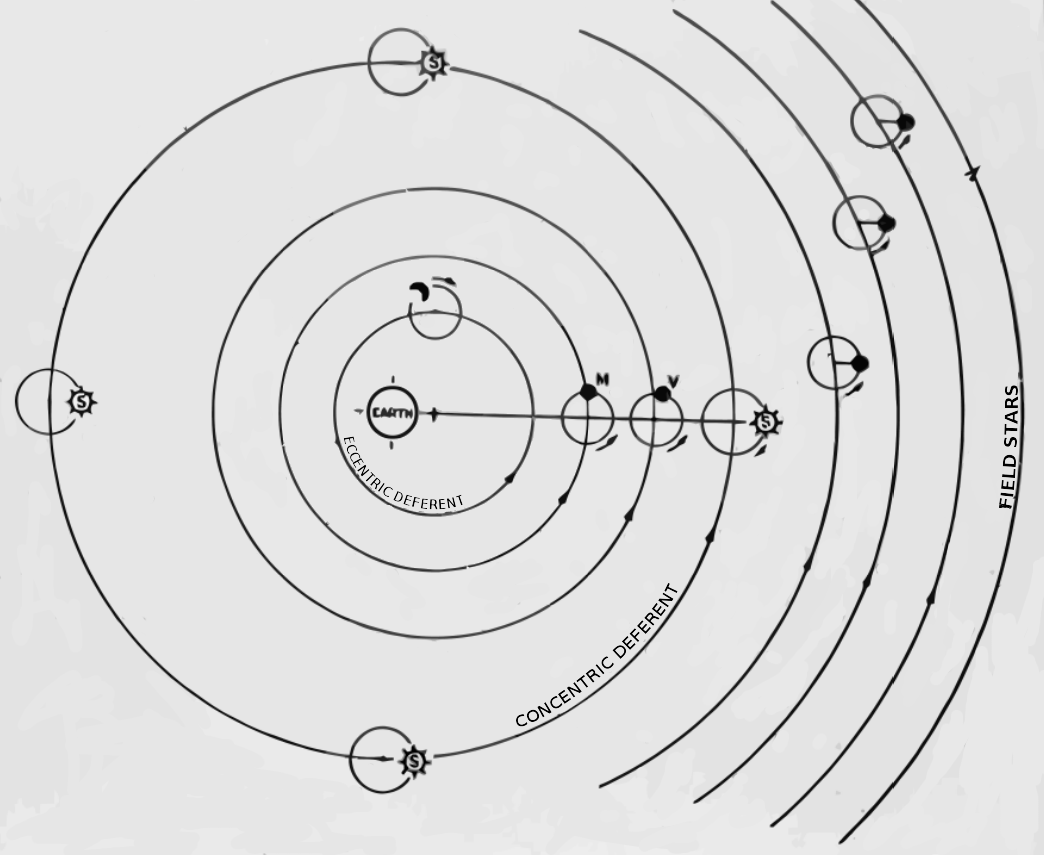
\includegraphics[width=0.45\linewidth]{Figures/0_PtolemaicModel.png}
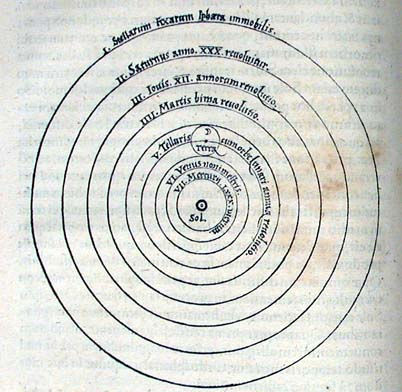
\includegraphics[width=0.38\linewidth]{Figures/0_CopernicusModel.jpg}
\caption{ Left: Depiction of the Ptolemaic geocentric system, the equant is not shown . Right: Copernicus illustration of his own heliocentric system, from \textit{De revolutionibus}. }
\label{Fig:0_PtolemyCopernicus}
\end{figure}



The astronomical evidence was, at the time, paradoxically against him. The apparent size changes of planets could not be measured yet, as well as stars parallaxes, contradicting heliocentrism. The idea of a moving Earth implied some effect on falling bodies (known today as coriolis effect) which were also not measurable at the time. Building on this apparent counter-evidence and on the work of indian astronomer Nilakantha Somayaji, Tycho Brahe, the most renowned astronomer of his time, proposed an alternative model known as the Tychonic system in the late 16th century \citep{ramasubramanian1998}. Brahe maintained the Earth as the center of the universe, circled by the sun, itself orbited by all other planets. The system was very efficient and was quickly adopted by the Church and considered in compliance with the Holy Scriptures.

However, the seed of heliocentrism was planted in european scientific minds. The idea exalted the impetuous and visionnary Giordano Bruno, who pushed the decentralization of Earth to the extreme, claiming stars were other suns, harboring other planets, which themselves could sustain intelligent life. For this, his rejection of catholic dogma and his vehement refusal of retractation, Bruno was burned at the stake on the Campo de Fiori in 1600. Bruno, the fiery dialectist, despised geometry and believed the mind alone could unravel any mystery. 

Johanes Kepler believed in geometry, in consistency and in observations. Ardent supporter of copernicism, he convinced Tycho Brahe to grant him access to his astronomical data, unsurpassed at the time. Focusing on the motion of Mars, Kepler, through trial and error, found out the planet was moving around the Sun following an ellipse. He formulated his first two laws of planetary motions. Further exploration led him to the third law. The three laws of Kepler were formulated, initiating the mathematisation of astronomy, and with it of all physics.

\subsection*{The Starry Messenger}


The father of modern astronomy, and precursor of modern science, Galileo Galilei was born in Pisa in 1564. For the first part of his scientific career, Galileo got famous for his lectures on mechanics and motion. Building on Buridan and Oresme's ideas, he expressed the mathematical form of free fall motion $ d = \frac{gt^2}{2}$. Galileo also formulated what was essentially the future first law of motion from Newton.

In 1609, his passion for scientific instruments led Galileo to build his own "dutch perspective glass", or telescope, a pioneering optical device from the netherlands. Once pointed at the sky, the device triggered an avalanche of observations who would forever bury the aristotelitian view of perfect and unchanged heavens. Moving Jupiter satellites, Moon craters and mountains, millions of stars in the Milky Way, these were consigned into \textit{Sidereus Nuncius} (Starry messenger), the first scientific publication of astronomical observations \citep{galileo1610}.

Strong advocate of copernicism, but lacking proper evidence, Galileo caused a large controversy with his 
\textit{Dialogue Concerning the Two Chief World Systems} published in 1632, a pamphlet against the ptolemaic system, presenting (arguably unintentionnaly) one of its advocates as a simpleton. Despite his friendship with the pope, he had to retract his work and reject copernicism. Galileo spent the rest of his life on house arrest. Observationnal evidence at the time was still on the side of geocentrism, but the extent of the backslash against Galileo showed the febrility of a Church having absorbed Ptolemy and Aristotle principle into its doctrine, in a time where the debate was shifting from theology to physics and observations.

The relativity of motion is often attributed to Galileo, as he includes it in its controversial pamphlet, stating that a traveller inside a ship sailing smoothly would not be able to tell he's moving. Thus, people could be standing on a moving Earth without feeling it. However, this thought experiment was nothing new at the time and had been a recurring theme of mechanical philosophy since Buridan. Oresme, Copernicus and Bruno had been building on the idea, expanding and improving it, developing over the centuries an implicit understanding of inertia, until Bruno actually gives it a name: \textit{virt\`u}. Galileo may have met Bruno himself, and had surely been influenced by his writings \citep{DeAngelis2015}. Galileo's formulation was clearer, and part of a larger understanding of motion, introducing the concept of reference frame. After Copernicus decentralized the Earth, Galileo decentralized human subjectivity itself, setting the scene for the revolution to come. 

\subsection*{On the shoulders of giants}

Isaac Newton is without a doubt the father of modern mathematical science. Admitted in Cambridge in 1661, Newton supplemented the -still- official aristotelitian teaching with more modern authors: Copernicus, Galileo, Kepler, and most of all, Descartes. The french philospher had a profound impact on the young student, rooting his love for mathematics and deductive reasoning. However, while Descartes showed disdain for experimentation, Newton was an acute observer of the natural world. 

In 1666, while in is mother's farm, having been forced out of Cambridge by the Plague, Newton began his reflexion on the motion of celestial bodies. He derived from Kepler's law that the Sun had to exert an inverse squared distance attraction on the planets. Extending the concept to the Earth, moon, and a famous apple, Newton found a way to verify his hypothesis, using data from Galileo mechanical studies on the strength of Earth attraction. The wrong estimate of Earth radius he used at the time introduced a discrepancy which put the young man off his \textit{gravitas} studies for 18 years.

Edmond Halley, astronomer and friend of Newton, having heard of Newton inverse squared law, urged him in 1684 to communicate his work the Royal Society. With a new accurate measure of Earth radius and confronted to a concurrent claim to his law from Robert Hooke \citep{Kramer1982}, Newton capitulated to Halley's eager enthousiasm and communicated his work in the famous \textit{Philosophiæ Naturalis Principia Mathematica} \citep{Newton1687}. Published at Halley's own expense, the Principia shook all of Europe. Newton had invented Calculus (in parallel of Leibniz) and applied it to derive the universal law of Gravitation.

\begin{equation}
F = G \frac{m_1.m_2}{r^2}
\end{equation}


Where:
\begin{itemize}
 \setlength\itemsep{-0.5em}
  \item[$F$] Gravitational attraction between object 1 and object 2
\item[$G$] Gravitational constant, $6.67408.10^{-11} m^3 kg^{-1} s^{-2}$ \citep{Pavese2015}
\item[$m_i$] Masses of object 1 and 2
\item[$r$] Distance between object 1 and 2
\end{itemize}

Though Newton was part of continuous line of geniuses and innovative minds building from each others, as he puts it "If I have seen further it is by standing on the shoulders of giants" \citep{Maury1992}, his input was truly revolutionnary. He made large advances in optics and mathematics, and created a consistent mathematical framework to compute motions, essentially founding modern science and sowing the seeds of the industrial revolution. This framework is summed up by Newton's three laws of motion (from recent translation \citealt{Cohen1999}):

\begin{quote}
Law I : Every body persists in its state of being at rest or of moving uniformly straight forward, except insofar as it is compelled to change its state by force impressed.
\end{quote}

\begin{quote}
Law II: The alteration of motion is ever proportional to the motive force impress'd; and is made in the direction of the right line in which that force is impress'd.
\end{quote}
 
 \begin{quote}
 Law III: To every action there is always opposed an equal reaction: or the mutual actions of two bodies upon each other are always equal, and directed to contrary parts.
 \end{quote}

The second law can be mathematically formulated in more modern terms:

\begin{equation}
\sum \bold{F} = \frac{d \bold{p}}{dt}
\end{equation}

Meaning the sum of all forces $\bold{F}$ applied to an object is equal to the time derivative of its momentum $\bold{p} = m.\bold{v}$.



\subsection*{The n=3 body problem}

As the Enlightenment brought a scientific revolution in many fields, I will now limit the discussion to the development of celestial mechanics, while acknowledging input from other fields.

While the two-body problem had been solved by Newton and expanded by Bernoulli in 1710 \citep{Barrow1997}, in the 18th century the three-body problem remained the object of much investigation and development. A general solution for the Earth-Moon-Sun system would have had applications on nautical astronomy and trans-continental navigation. Extended analytical work by d'Alembert, Clairaut, Euler and Lagrange led to the development of early families of approximate solutions or exact solutions to special cases.

From 1773 to 1793, Joseph-Louis Lagrange, helped by his invention of Lagrangian mechanics, would make a lot of advances on the three-body problem. He introduced the concept of potential and discovered libration points (later known as Lagrange points). In the same time, Pierre-Simon de Laplace proved the stability of the solar system using a newly developped perturbation theory. The solar system dynamics were being unraveled, with finely tuned perturbation computation, but the general three-body problem remained unsolved.

In 1888, Henri Poincaré, greatest mathematician of his time, submitted an entry to a contest organized by the King of Sweden Oskar II. The goal was to determine a usable solution to the n-body problem, for any given n. While Poincaré does not submit a complete solution, he wins the contest by presenting an in-depth exploration of the phase-space of the restricted three-body problem, which would later give rise to the Chaos theory ,see \cite{Yoccoz2010}. Poincaré managed to prove that the three-body problem had no  solution involving simple functions.

Contrary to popular belief, the three-body problem \textit{has} a solution, it was derived by Karl F. Sundman in 1912 \citep{Sundman1912}. However, any attempt to obtain accurate trajectory predictions would face tremendous convergence time and is in practice unusable \citep{Beloriszky1930}.

It is interesting to note that Elis Str\"omgren performed by-hand calculation of a three-body system, see \cite{Aarseth2003,Stromgren1909}, prefiguring the advent of numerical orbit computation.

\subsection*{The n$>$3 body problem}

\begin{quote}
"The Sun attracts Jupiter and the other planets, Jupiter attracts its satellites and similarly the satellites act on one another."
\end{quote}

By this sentence from the \textit{Principia}, Newton formulates the n-body gravitational problem, an arbitrary number of massive bodies all interacting gravitationally, for the solar system. The "n$>$3-body" problem didn't receive a lot of attention at first, as the unruly three-body problem was on everyone's mind, and a n$>$3-body problem seemed abstract, the solar system example being appropriatly dealt in approximations.

In 1764, Charles Messier resolved individual stars in Messier 4, a globular cluster, hundreds of thousands of stars grouped together. Many new clusters were to be found afterwards, extending the catalog of real-life n-body systems. However, nothing was known of their kinematics, the stars were somehow suspended motionless in the sky. This was the case until the advent of Doppler spectroscopy, which allowed astronomer to measure stars velocities \citep{Doppler1842}. Stellar dynamics had begun.

The n$>$3-body problem was still inaccessible, so scientists like James Jeans and Arthur Eddington decided to take the problem from the other hand, and took advantage of the large number of stars. Inspired by \cite{Poincare1906}, both astronomers applied the statistical theory of gas to stellar systems, founding the field of stellar dynamics \citep{Jeans1916,Eddington1916}.

An interesting experiment was conducted by \cite{Holmberg1941} to understand the collision of two stellar systems (galaxies). With too few points to warrant a statistical approach, and before the rise of numerical integration, Holmberg modelled two galaxies with dozens of lightbulbs and photocells, measuring the attractive force with the amount of light received in each direction, taking advantage of the inverse squared fall of luminosity with distance, akin to gravity.

\subsection*{The numerical age}

The first numerical N-body computations were performed by Sebastian Von Hoerner in 1959 when visiting the University of T\"ubingen, on a Siemens 2002, a cutting edge calculator at the time. The very first had N=4. Then, Von Hoerner, back in Heidelberg, worked his way up to 16 stars, then 25, programming and debugging on punch cards. This story was told by Von Hoerner himself in \cite{VonHoerner2001}. He very quickly realized the importance of binary stars and their impact on computations. He was also able to confirm some theoretical prediction on cluster dynamics, and found an interesting radial density profile with a center cusp \citep{VonHoerner1960,VonHoerner1963}.

\begin{figure}
\label{Fig:N_increase}
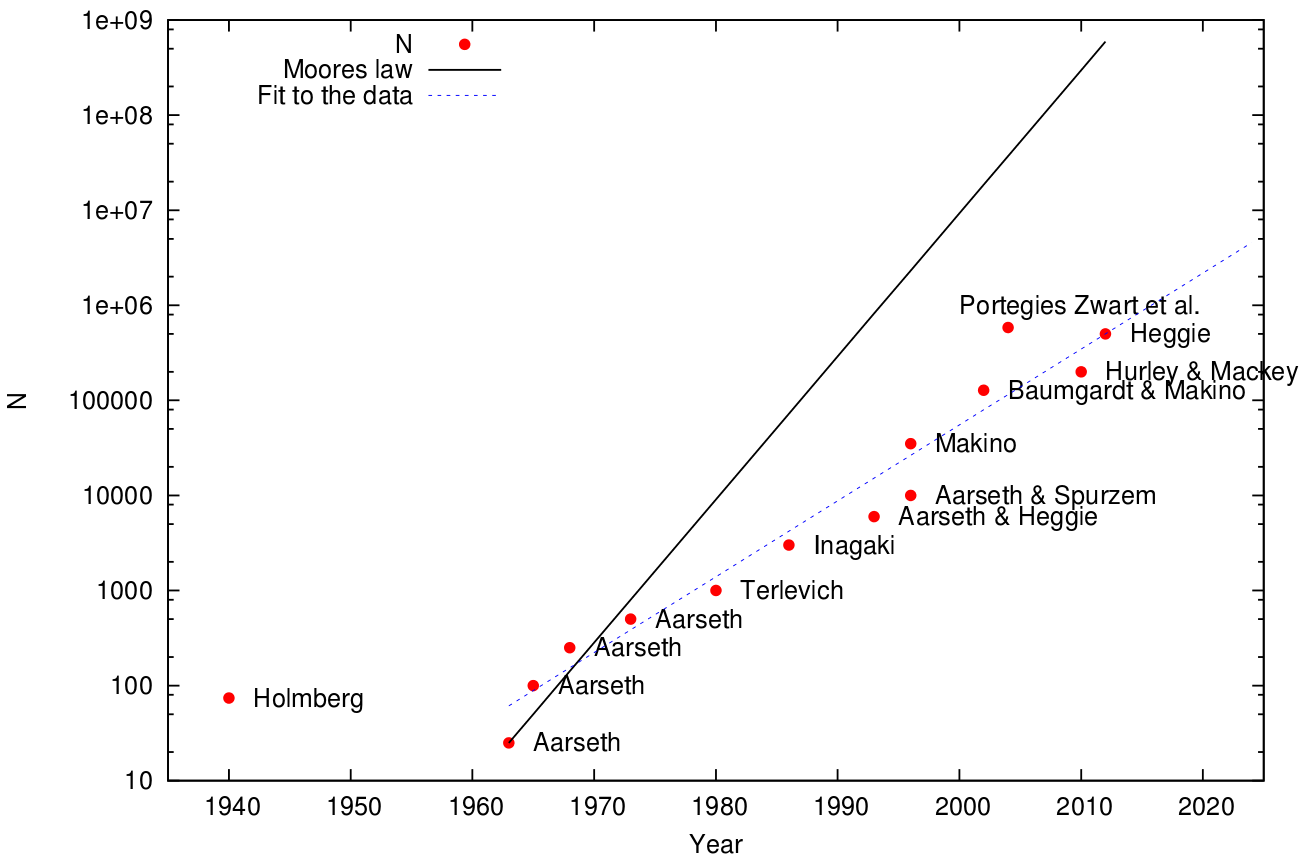
\includegraphics[width=0.9\linewidth]{Figures/0_N_increase.png}
\caption{The evolution of the number of particles in N-body simulations. Solid line shows the Moore law. The figure was taken from \protect\cite{Bedorf2012}. }
\end{figure}


There was two ways to increase the number of stars in simulations: buy a better computer or improve the algorithm. Sverre Aarseth got invested in the second path, which would take over his scientific life. Aarseth pioneered the use of individual time-step, changing the rate at which particles positions are updated, gravitationnal softening, allowing convergence for close approach, and polynomial prediction for force calculations \citep{Aarseth1964}. As power and optimization grew, investigations expanded, such as the interaction star-gas \citep{VanAlbada1968a} and binary formation \citep{VanAlbada1968b}.

The 1970s brought two new important optimisation methods: KS regularization of close pairs \citep{Aarseth1972} and Ahmad-Cohen neighbour scheme \citep{AhmadCohen1973}. The number of stars in simulations kept growing, reaching 1000 with \cite{Terlevich1980} and materializing into the \textit{NBODY5} integrator. At this point various methods departing from a pure collisional calculation began to emerge, such as the simplified distant interaction with the \cite{BarnesHut1986} tree algorithm.

To go beyond the regular improvement of computing power with time, a group of japanese researchers, among whom Junichiro Makino, designed and built special purpose hardware for many-body problems: GRAPE \citep{Ebisuzaki1990,Ito1991}. These cards vastly improved the speed of nbody simulations and were a milestone on the road to the parallelization of computing. With the force calculation directly implemented in the hardware, GRAPE dominated the field for 15 years.

The latest technological leap in Nbody simulations came from graphic cards, see \cite{Bedorf2012} for a more detailed historical perspective. Graphical Processing Units, or GPU, were originally designed for computer games visual rendering, applying the same transformations to a lot of pixels at the same time. These made them very efficient parallel computing machines for physics. Interest in GPU computing started to grew in the 2000s \citep{Nyland2004,Elsen2006,SPZ2007} until the advent of usable GPU programming languages, like CUDA, in the late 2000s. At this point GPU were more efficient than GRAPE hardware for force calculation. Keigo Nitadori and Sverre Aarseth developped a GPU-accelerated version of the latest NBODY code, NBODY6, in 2012 \citep{Nitadori2012}.

Last year, 329 years after the publication of the \textit{Principia}, a collisional nbody simulation of one million stars was performed with a modified version of NBODY6 running on GPU \citep{Wang2015}. Computers have made it possible for humans to study systems of incredible scales in space and time, only using the universal law of gravitation. N-body numerical integrators are the culmination of centuries of scientific development on the motion of massive bodies.



\newpage
\section{Star clusters}

\subsection{What are star clusters ? And why study them ?}

The widest definition possible for a star cluster is "An area of the sky with visibly grouped stars". However, this includes binary stars and galaxies. We are interested in intermediate systems, such as open clusters, globular clusters or associations, in which stars are, if not bound, at least under direct mutual gravitational influence. These objects can either dissolve in less than a million year or remain bound for billions of years.

Clusters are the result of bursts of star formation in Giant Molecular Clouds. All stars within a cluster were born approximately at the same time, which explains the sustained interest of the scientific community for star clusters for more than a century. They are the best laboratories of stellar physics available to us: a large population of stars sharing the same age and distance to Earth. The age of the cluster can be derived from the most massive stars in the population, as stars have lifetimes inversely correlated with their mass. Overall, integrated spectral features from all members of a star cluster can provide a wealth of information.


\begin{figure}
\center
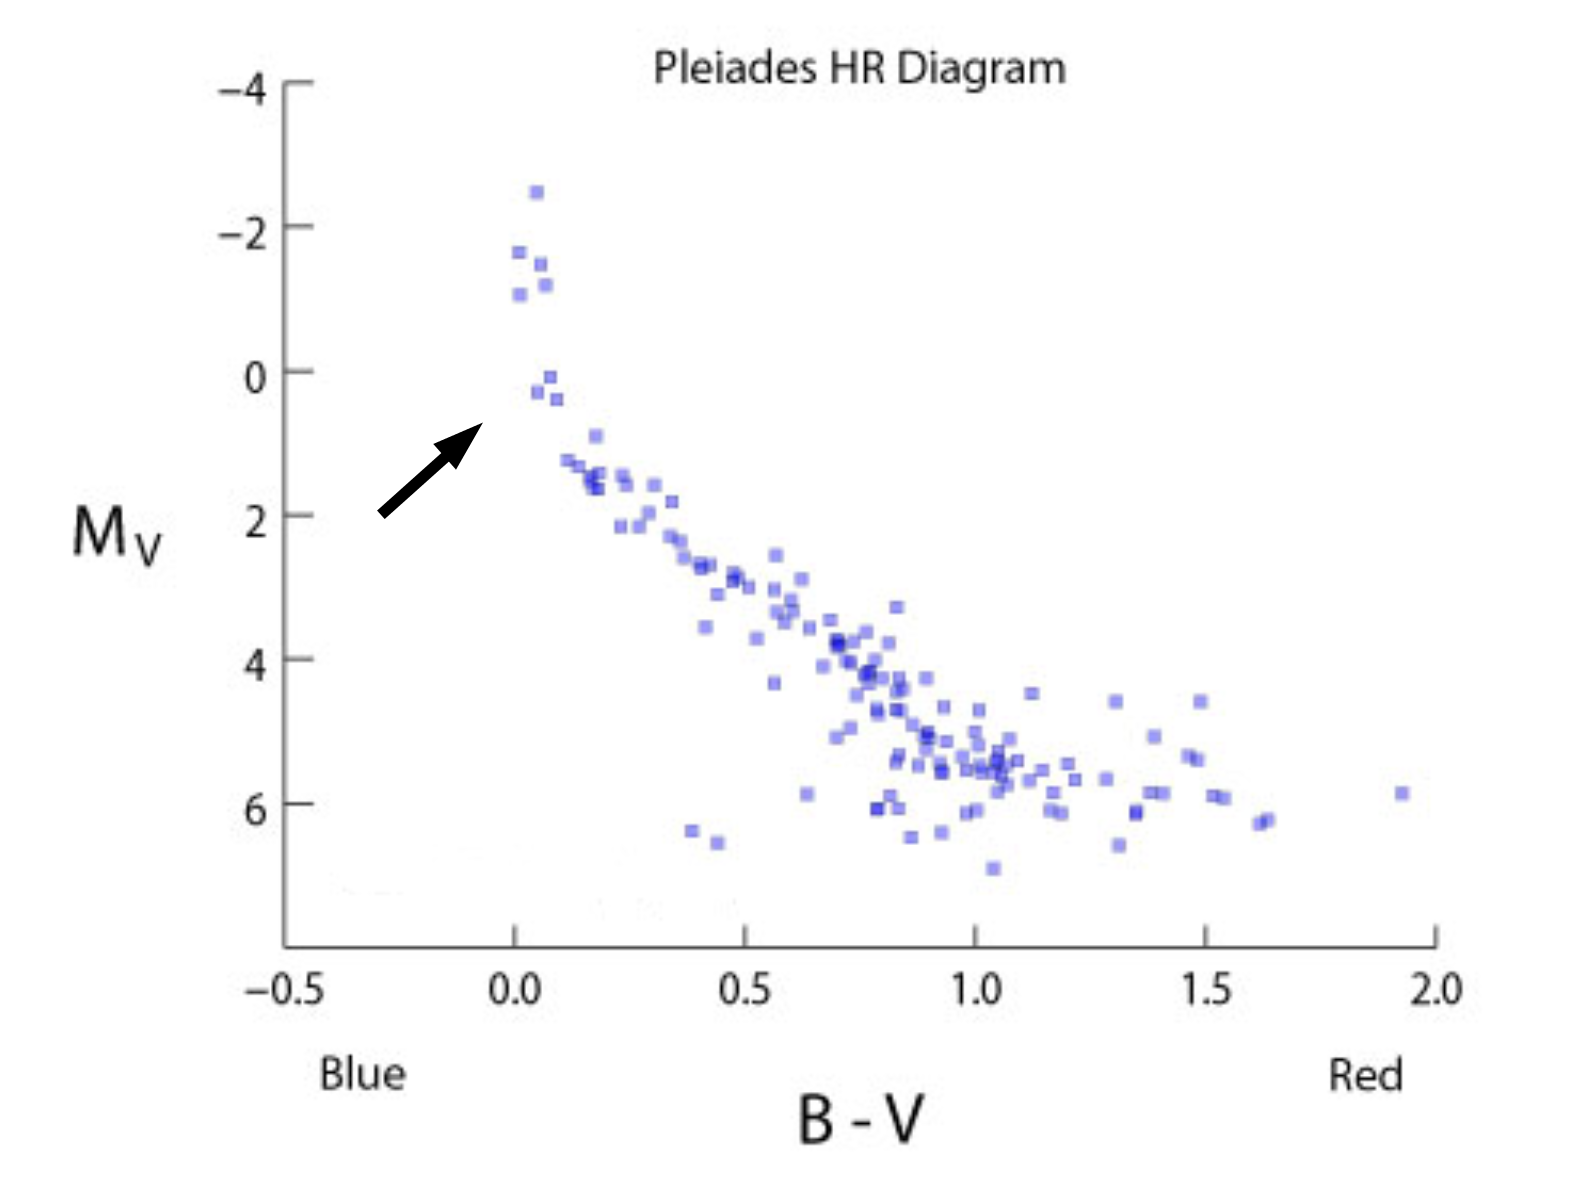
\includegraphics[width=0.45\linewidth]{Figures/0_HRDiagram_Pleiades.png}
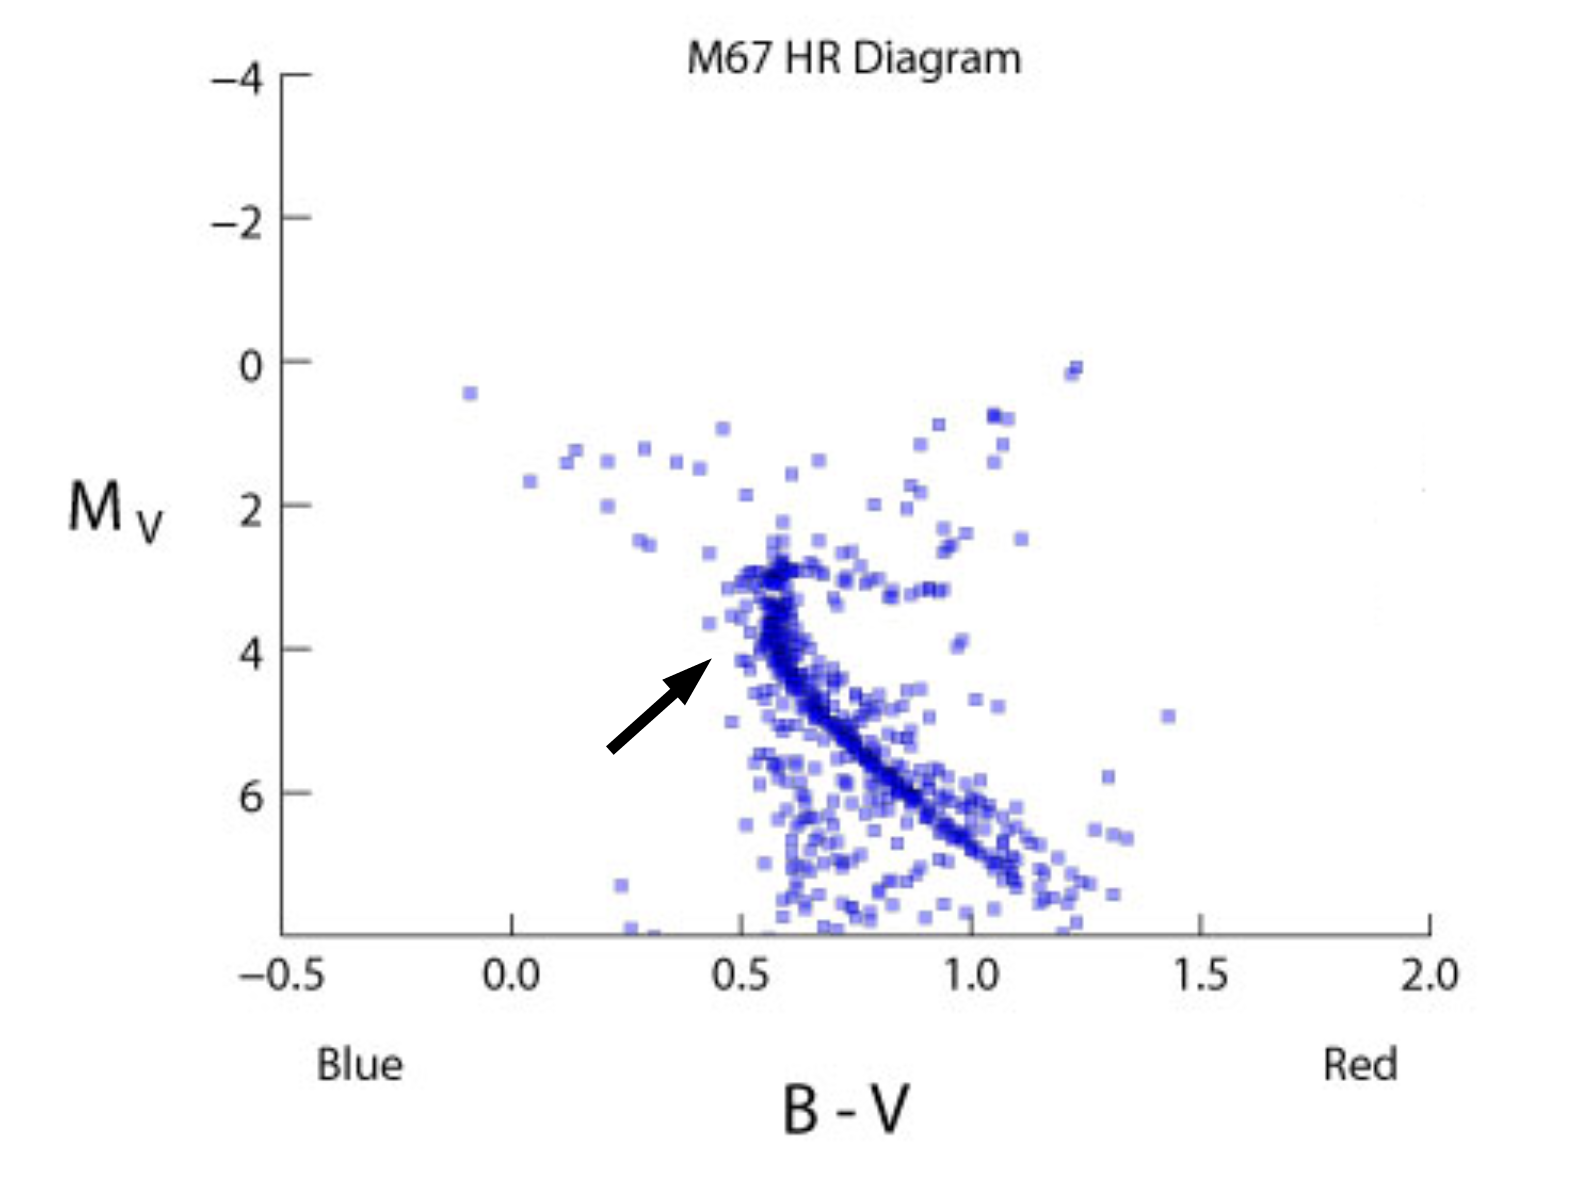
\includegraphics[width=0.45\linewidth]{Figures/0_HRDiagram_M67.png}
\caption{Hertzprung-Russel diagram of the Pleiades and M67. An arrow points at the Main-Sequence turn-off for each cluster. The figures were taken from the \href{http://www.astrophysicsspectator.com/topics/stars/HertzsprungRussellClusters.html}{Astrophysics Spectator} website and data can be found in \protect\cite{Stassun2002,Kharchenko2004}  }
\label{Fig:0_HR}
\end{figure}

One example is the ability to date a cluster, thus its members, through the main-sequence turn off. On figure~\ref{Fig:0_HR} is shown the Hertzprung-Russel diagram for two different clusters: The Pleiades and M67. The HR diagram shows the luminosity of the star versus its color, redder on the right, bluer on the left. Stars spend most of their life on the Main Sequence, with the most massive, luminous blue stars on the left, and red fainter smaller stars on the right. Massive stars have shorter lives and depart from the main sequence before small stars. Looking at the Main Sequence turn-off in the HR diagram of a cluster tells us the mass of the stars currently leaving the MS, which gives its age and that of all other stars. As seen on the figure, the Pleiades are younger (100Myr) than M67 ($\sim$ 4 Gyr) as the stars leaving the MS are more massive.

Star clusters are historically divided into two main categories: globular clusters and open clusters. As observationnal techniques improve, categories tends to blend into a spectrum of size, age, and dynamical state, with Young Massive Clusters, embedded clusters, associations.






\subsubsection*{Globular clusters}

Globular clusters are old and massive stellar systems. Most of them are older than 10 Gyr and more massive than $10^4~M_\odot$. They only contain stars, with no dust or gas. The 150 known globular clusters in the Milky way are scattered in the disk and the halo. Due to their age, GCs are dynamically evolved. Introducing the relaxation time, defined in \cite{BT} by:
\begin{equation}
\label{Eq:0_relaxation}
t_{relax} = 0.1 \frac{N}{logN} t_{cross} = 0.1 \frac{N}{logN} \frac{R_{hm}}{\sigma}
\end{equation}

with $t_{cross}$ the crossing time, defining the time a star takes to cross the system and $\sigma$ the internal velocity dispersion. The relaxation time is the time it takes for a system to erase its initial condition, perturbation per perturbation. GCs have a relaxation time of about a Gyr, they are relaxed systems. Various models have been put forward for the structure of GCs, the King \citep{King1966} and Plummer \citep{Plummer1911} models are the most widely used.




\begin{itemize}

\item 47 Tucanae (NGC 104) is one of the most massive known globular cluster in the Milky Way. It is estimated to contain about 1.5.$10^6~\Mo$ and to be 13 Gyr old\citep{Forbes2010}. Its core is extremely dense, as many GCs, with a central density up to $10^6 \Mo/\textrm{pc}^3$. Such a concentration of stars is a favorable environment for stellar collisions, which create what is called \textit{stellar exoticae}, stellar object not following the standard evolutionnary path, such as blue stragglers. Blue stragglers are stars too luminous and too massive compared to the age of the cluster, likely formed out of colliding stars. 47 Tuc exhibits a population of such objects, as well as others: Cataclysmic variables, X-ray binaries, etc. These are the direct consequence of the very dense environment of globular clusters such as 47 Tuc.

\item Messier 12 (NGC 6218) is on the light end of the mass spectrum with 9.$10^4~\Mo$ \citep{Marks2010}. Such a low mass is however thought to be due to the cluster's dynamical history. Globular clusters have orbits around the galaxy, some more dangerous than others. For example Palomar 5 is currently disappearing after violent encounters with the galactic center. A study by \cite{DeMarchi2006} showed M12's orbit probably also passes close to the galactic center. Subjected to the strong tidal forces of the galactic bulge, M12 would have lost about 4/5 of its original mass. This scenario is backed by the mass function of M12. The mass function is the distribution of stellar masses, and its slope is thought to be more or less universal, though it appears unusually flat in M12. The tidal shock would have preferentially depleted low mass stars, as a process known as mass segregation tends to have massive stars sink at the center and low-mass stars overpopulate the outskirts of the system. 

\item NGC 2808 is reported to contain 1.4 $10^6~\Mo$ \citep{Boyles2011}. NGC 2808, as all others GCs, had long been thought to have an homogeneous stellar population. Yet, a study by \cite{Piotto2007} showed NGC 2808 contained at least three different stellar sequences. As this cannot be explained by the natural age spread arising from a continuous star formation at the birth of the cluster, such observations have far-reaching implication on its formation scenario, and those of many GCs with multiple populations. Several hypothesis are being explored, such as GCs being the outcome of mergers \citep{Pasquato2016} or a sequence of distinct star forming events \citep{Dantona2016}, with no consensus for now.

\end{itemize}


\begin{figure}
\label{Fig:0_GlobularClusters}
\center
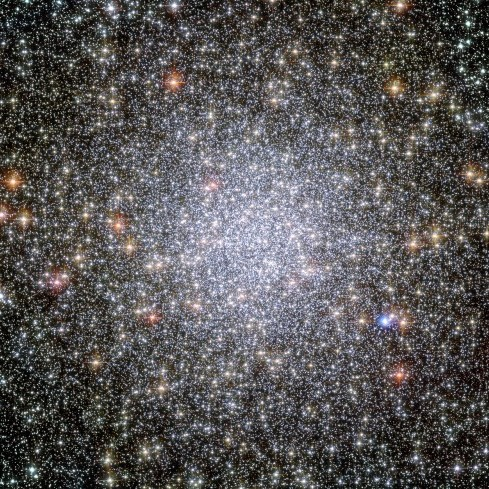
\includegraphics[width=0.3\linewidth]{Figures/0_47Tuc.jpg}
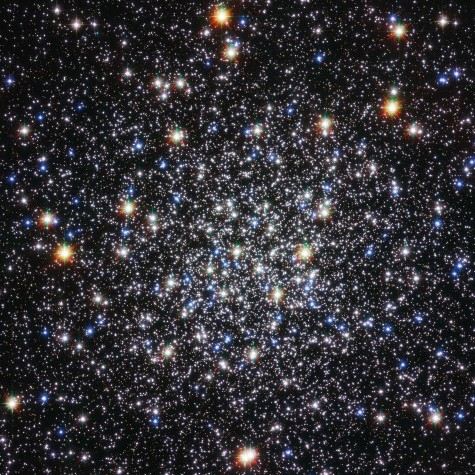
\includegraphics[width=0.3\linewidth]{Figures/0_M12.jpg}
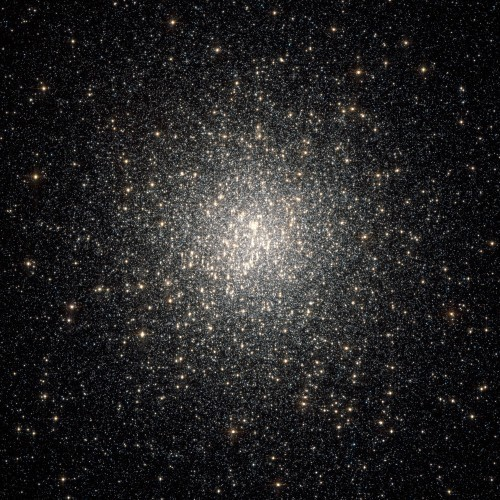
\includegraphics[width=0.3\linewidth]{Figures/0_NGC2808.jpg}
\caption{From left to right: 47 Tucanae, Messier 12 and NGC 2808. Credits: ESA/Hubble. }
\end{figure} 


\subsubsection*{Open clusters}


\begin{figure}
\center
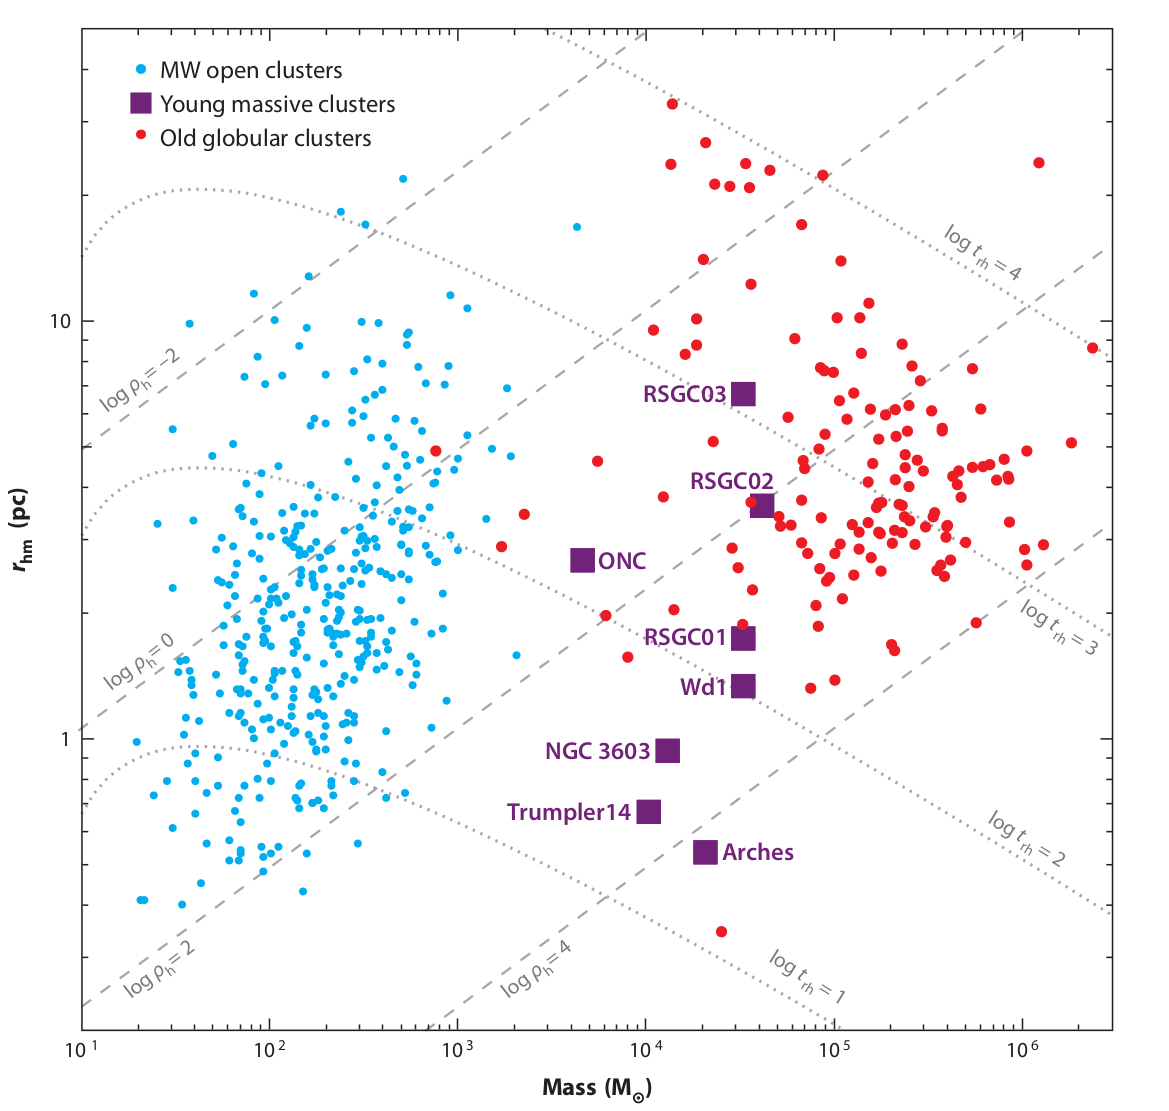
\includegraphics[width=0.65\linewidth]{Figures/0_MassRadiusClusters.png}
\caption{Radius-Mass Diagram for Milky Way clusters. Blue dots are open clusters, red dots Globular clusters and purple squares show Young Massive Clusters. Dashed lines show constant density within half-mass radius $\rho_h = 3M/8\pi r^3_{hm}$ and dotted lines show constant relaxation time. The plot was taken from the review \protect\cite{PortegiesZwart2010}.}
\label{Fig:0_SPZ}
\end{figure}


Open clusters are lighter objects, rarely more massive than $10^3 \Mo$. They are also younger, typically no older than a Gyr. In fact, Open Clusters are thought to be very volatile, with the vast majority not surviving beyond 100Myr. Causes of disruption include internal two-body evolution and tidal shocks from passing massive clouds on nearby orbits.



\subsection{Formation in Giant Molecular Clouds}

\subsection{Early dynamical evolution}

\subsection{Binary stars in clusters}









\newpage
\section{NBODY6}


NBODY6 is the second youngest iteration of the NBODY family, a suite of n-body integrators created by Sverre Aarseth. It can compute the gravitational interaction between up to 128,000 stars in a collisional fashion, meaning there is no softening of the potential, at any scale. This allows for very close binaries to form and remain in the system. To achieve its impressive performances, NBODY6 relies on several optimization technique which have been first developed in the 1960s and 1970s, and improved ever since. Here will be developped four major features of NBODY6, in chronological order of their implementation: block time-step, KS-regularization, Hermite scheme and Ahmad-Cohen neighbour scheme. A full description can be found in Sverre Aarseth's book \citep{Aarseth2003}.% Inspiration for this section should be credited to the user manual of NBODY6++, written by Emil Khalisi and Rainer Spurzem.

\subsection{Block time-step}
 
In the first Nbody simulations, the system was integrated with an universal time-step, determined by the most accelerated star. A star in the outer regions of the cluster with a small velocity did not need to be updated that often. One of the first improvement  was the introduction of individual time-step: each star is attributed its own time-step, depending on the force that is applied to it and its derivative:

\begin{equation}
\Delta t_i =  \eta \sqrt{\frac{ |\bold{F_i}||\bold{F^{(2)}_i}| + |\bold{F^{(1)}_i}|^2 }{|\bold{F^{(1)}_i}||\bold{F^{(3)}_i}| + |\bold{F^{(2)}_i}|^2}}
\end{equation}
 
With $\bold{F}^{(j)}_i$ begin the j-th derivative of the force applied to particle i and $\eta$ a user-defined accuracy parameter. Such a complex formulation is the result of extensive tests and is quite robust for many special cases. Individual time-steps leads to desynchronized particles, hence the need to interpolate the positions of other particles to compute $\bold{F}_i$, which was achieved through fourth-order polynoms.
 
 To limit the amount of desynchronization, block-time steps were introduced. Instead of having as many time steps as particles, one only allows quantized power of 2 of an initial time step. $\Delta t_0$,$\frac{\Delta t_0}{2}$, $\frac{\Delta t_0}{4}$, $\frac{\Delta t_0}{2^i}$. All time steps are then commensurate and regularly fall back on the same time steps, minimizing the amount of interpolation during the force calculations.
 
\begin{figure}
\label{Fig:blocktimesteps}
\center
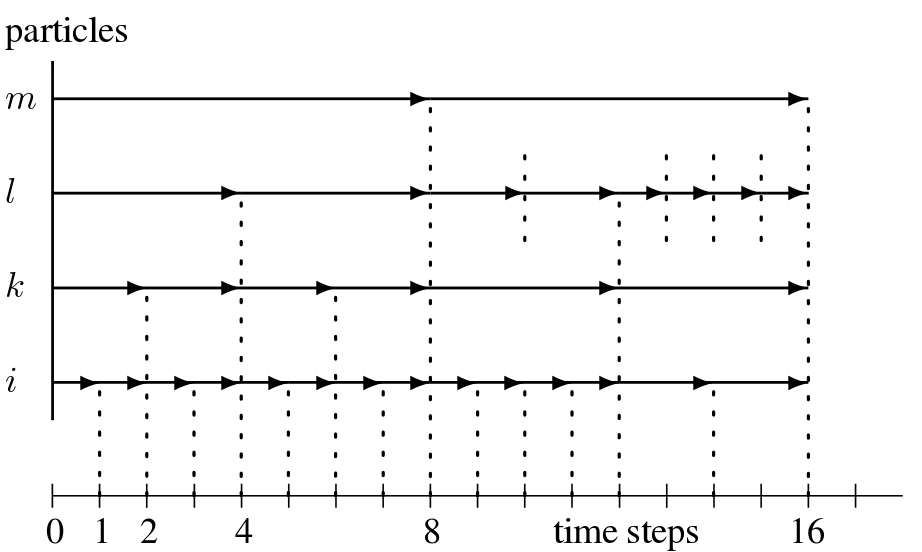
\includegraphics[width=0.6\linewidth]{Figures/0_block_timesteps.png}
\caption{Illustration of block time steps on 4 particles. Particles get their positions updated for each arrow symbol, common time steps are shown as vertical dotted lines. Figure from NB6++ User Manual. }
\end{figure} 
 
 
\subsection{KS-regularization}



\subsection{Hermite prediction scheme}

\subsection{Ahmad-Cohen neighbour scheme}




\newpage
 \section{Young star clusters}












    
    \part{The fragmented model and its evolution}
    %%%%%%%%%%%%%%%%%%%%%%%%%%%%%%%%%%%%%%%%%%%%
% Chapitre 1
%%%%%%%%%%%%%%%%%%%%%%%%%%%%%%%%%%%%%%%%%%%%

\chapter{The Hubble-Lema\^itre fragmented model} 
\label{ChapterHL}

\section{How to build a Hubble-Lema\^itre model}

\subsection{Initial state}

The first step to obtain a HL-fragmented model is to build an uniform sphere model. The N stars, depending on the required membership, have to be distributed randomly in space inside a certain radius, producing an uniform density. This can be achieved by sampling separately the distance to the center and the angular position of each star, in a method analog as used in \cite{Aarseth1974} for a Plummer model. The distance to the center should be sampled from the function:

\begin{equation}
f_R(X) = R_0 X^2
\end{equation} 

With $R_0$ the bouding radius and X a random variable following a uniform probability law between 0 and 1. A direct uniform law for the radius would overpopulate the outer regions. The angles $\phi$ and $\theta$, respectively azimuthal and polar angle in the physics convention, should be sampled from:


\begin{align}
f_\phi(X_1) & = 2\pi X_1\\
f_\theta(X_2) &= \arccos{ (X_2) }
\end{align}

With $X_1$ following a uniform probability law between 0 and 1 and $X_2$ between -1 and 1. The cartesian coordinates are then found:

\begin{align}
x &= R \sin{\theta} \cos{\phi}\\
y &= R \sin{\theta} \sin{\phi}\\
z &= R \cos{\theta} \\
\end{align}

The N particles are then homogeneously distributed in space in a sphere of radius $R_0$. The next step is to attribute velocities. Unlike other models like the Plummer model, the velocities are here straightforward. We use the well known velocity field of neighbouring galaxies: velocities are radial from the Milky Way, larger with increasing distances, taking the form:

\begin{equation}
\label{Eq:1_Hubble}
\bold{v} =  \textrm{H}_0 \bold{r},
\end{equation}

with H$_0$ being an equivalent of the well-known Hubble parameter. For historical accuracy, I added the name of Georges Lema\^itre when I named my model. It has now been shown that the astronomical observations of redshifted galaxies and its interpretation as the consequence of an expanding universe predated Hubble's paper \citep{Hubble1929}. Georges Lema\^itre had published his conclusion on an expanding universe two years earlier \citep{Lemaitre1927}. The account of this can be found in \cite{Kragh2003,VanDenBergh2011} and \cite{Freeman2015}.

An appropriate H$_0$ to obtain a fragmented subvirial model has to be inferior to 1.4 (see next section). The model obtained from this is then evolved through a nbody integrator, which in my case is NBODY6.


\subsection{Fragmentation}

The cluster expands, driven by the initial Hubble-Lema\^itre velocity field. During this expansion, poissonian fluctuation in density from the uniform model starts to grow: the part of the cluster with more mass initially attract more stars, forming clumps, clumps merge, spontaneously building substructure. These clumps will be analyzed in another section. If H$_0$ is well chosen, the expansion stops at some point, the apex, at which the initial kinetic energy has been spent and converted to potential energy: the cluster is now larger, substructured and subvirial, about to collapse. The apex time $t_a$ of the end of the expansion and the critical value of H$_0$ can be derived from Newton's second law applied to an expanding spherical shell of matter.

We start from a uniform sphere of radius $R_0$, total mass $M$. We consider spherical shells as mass elements, situated at distance $r$ from the origin. As previously said, they are attributed a radial velocity following (for the shell at $r=R_0$) $\vec v_0 = \Hub_0 \vec R_0 = \Hub_0 R_0 \vec u_r$. We want to follow the radial motion of the last shell of mass m, situated at $R$ from the origin. Newton's second law gives:


%\begin{equation}
\begin{align}\label{eq:newton}
m \frac{dv}{dt} & = - \frac{G M m}{R^2}
\end{align}
%\end{equation}

By multiplying on both sides by $v$ and integrating between a given time and $t=0$, one finds:

\begin{equation}
v^2(t) - v^2_0 = 2GM \left( \inv{R} - \inv{R_0} \right)
\end{equation}

Which becomes, by taking $\nu = v/v0$,  $x= R/R0$ and defining:

\begin{equation}
\label{Eq:1_Estar}
E_\ast = \frac{2GM}{R_0 v_0^2}
\end{equation}
which is a dimensionless measure of the total energy of the system:

\begin{equation}
\nu^2  = 1 + E_\ast \left( \inv{x} - 1 \right) .
\end{equation}

The evolution of the system has 3 outcomes, depending on the value of $E_\ast$:
\begin{itemize}
\item $E_\ast<1$ The velocity is always strictly positive as the system expands ($x->\infty$). The system is unbound.
\item $E_\ast=1$ The velocity approaches zero as the system expands. The expansion "stops at an infinite radius". The system is marginally bound.
\item $E_\ast>1$ The velocity reaches zero for a finite radius, the system is bound and will collapses back on itself once the expansion stops. 
\end{itemize}

Using H\'enon units, $G=1$ and $M=1$, and we choose $R_0$=1. Which gives a critical value $E_*$ to have a bound system: $E_* = \frac{2}{\Hub^2_0} < 1$. This means to have a bound system, which stops expanding at some point, one must have $\Hub_0 < \sqrt{2}$.
We only consider in the following the case in which $E_\ast<1$. We have the expression

\begin{equation}
\nu = \sqrt{1+E_\ast\left(\inv{x} - 1\right)}
\end{equation}

Taking the time derivative gives:

\begin{equation}
\frac{d \nu}{dt} = - \frac{E_\ast}{2 x^2} \left[ 1 + E_\ast\left(\inv{x} -1\right)\right]^{-\frac{1}{2}} \frac{dx}{dt}
\end{equation}

Combining this with (\ref{eq:newton}), one obtains:

\begin{equation}
\frac{dx}{dt} = \Hub_0 \sqrt{1+ E_\ast\left( \inv{x} -1\right)}
\end{equation}

which can be rewritten, using $\tilde{\Hub_0} = \Hub_0 \sqrt{E_\ast-1}$ and $x_t=\frac{E_\ast}{E_\ast-1}$

\begin{equation}
\frac{dx}{dt} = \tilde{\Hub_0} \sqrt{\frac{x_t}{x}-1}
\end{equation}

$x_a$ being the extent of the maximum expansion as we assumed a bound system. The subscript a is for apex. If we choose the notation $u = \frac{x}{x_a}$:

\begin{equation}
\sqrt{\frac{u}{u-1}} \frac{du}{dt} = \frac{\tilde{\Hub_0}}{x_a}
\end{equation}

We know that $x$ varies from 1 to $x_a$, thus $u$ varies from $1/x_a$ to 1. We can then make the change of variable $u = \sin^2\theta$ and separate the variables:

\begin{equation}
\sqrt{\frac{\sin^2\theta}{1-\sin^2\theta}} 2 \sin\theta \cos\theta d \theta = \frac{\tilde{\Hub_0}}{x_a} dt
\end{equation}

which becomes after simplifications:

\begin{equation}
\label{Eq:1_integrand_theta}
[ 1 - \cos(2\theta)]d\theta = \frac{\tilde{\Hub_0}}{x_a} dt .
\end{equation}


We now integrate the expression from $t=0$ to $t$, the time at which the expansions stops and $x$ reaches $x_a$ (wich implies $u_a = 1$ and $\theta_a = \pi /2)$:

\begin{align}
\int^{\pi/2}_{\theta_0} [ 1 - \cos(2\theta)]d\theta  & = \int^t_0 \frac{\tilde{\Hub_0}}{x_a} dt\\
\frac{\pi}{2} - \theta_0 + \frac{\sin(2\theta_0)}{2} & =  \frac{\tilde{\Hub_0}}{x_a} t\\
\pi - 2 \theta_0 + \frac{2}{\sqrt{x_a}}\sqrt{1-\inv{x_a}} & = 2 \frac{\tilde{\Hub_0}}{x_a} t 
\end{align}

which boils down to the expression of the time at which the expansion stops:

\begin{equation}
t_a = \frac{E_\ast \left(\frac{\pi}{2} - \theta_0\right) + \sqrt{E_\ast-1}}{\Hub_0 (E_\ast-1)^{-\frac{3}{2}}}.
\end{equation}

Recalling the quantities:
\begin{align}
E_\ast = \frac{2GM}{R_0 v_0^2}        &;  & x_a=\frac{E_\ast}{E_\ast-1}  &;  &\theta_0 = \sin^{-1}\left(\inv{\sqrt{x_a}}\right)  
\end{align}

See figure \ref{Fig:apextime} for the value of $t_a$ as a function of \Hub$_0$

\begin{figure}
\center
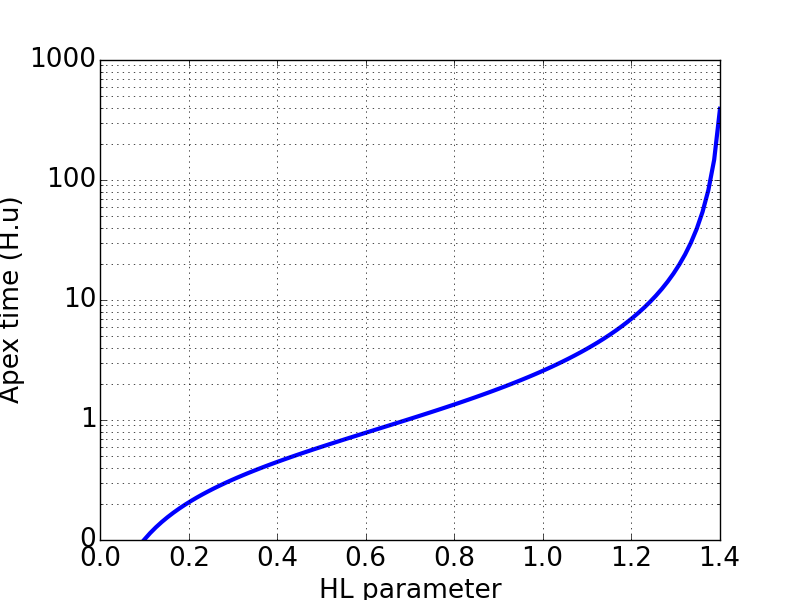
\includegraphics[width=0.7\linewidth]{Figures/1_apextime.png}
\caption{Theoretical values of the apex time, at which the system stops expanding, as a function of initial HL parameter, which tunes the strength of the initial expansion.}
\label{Fig:apextime}
\end{figure} 





\section{The growth of overdensities: analytical study}



\subsection{Working equations}



\begin{table}
\begin{center}
\caption{Summary of main variables.}
\label{Tab:identities}
\begin{tabularx}{\columnwidth}{rl}
\hline
$E$ & Total system energy \\
$E_*$ & Dimensionless total energy \\
$W$ & Total potential energy \\
$E_k$ & Total kinetic energy\\
$\cal M$ & Total system mass\\
$R_o$ & Initial bouding radius\\
$\Hub_0$ & Initial Hubble parameter\\
$v_o$ & Initial velocity at bounding radius\\
$\Hub$ & Variable Hubble parameter\\
$\tau$ & Dimensionless time\\
$x$ & Comoving spatial coordinate\\
$a(t)$ & Rescaling function\\
$\theta$ & Calculation angle\\
$\nu(\tau)$ & Dimensionless velocity $1 + E_*(1/a(\tau)-1)$\\
$\xi$ & Radial displacement from comoving \\
$\delta\rho,\delta M,\delta\rho$ & Perturbed quantities\\
$\mu(\tau)$ & Central point mass\\
$\eta$ & Peculiar velocity $d\xi/dt$\\
\hline
\end{tabularx}
\end{center}
\end{table}

During the expansion and in the mean-field approximation, the mass inside any shell of radius $r(t)$ is conserved as they move outwards. The position of a mass element is known in parametric form from a rescaling of its initial coordinates and we may write 

\begin{align} 
\bold{r}(t) &= a(t)\bold{x}\\
\bold{v}(t) &= \dot{a}\bold{x} = \Hub(t)\bold{r} 
\end{align} 

 where $\bold{x}$ is a co-moving coordinate of position, and $a(t)$ is a dimensionless function of time. The flow is homological and no shell-crossing takes place. It is convenient to introduce a dimensionless time $\tau$ such that 
 
 \begin{equation} 
 \label{Eq:1_taudef}
  t = \frac{\tau}{\Hub_0}.
 \end{equation} 
 
  We then have from equation (\ref{Eq:1_integrand_theta}):
\begin{equation}
\label{Eq:1_Expansion} 
\left. \left[ \frac{ E_\ast}{E_\ast -1} \right]^{\frac{3}{2}} \, \left[ 2\theta - \sin{2\theta} \right]\, \right\vert_{\theta_o}^\theta =  2\sqrt{E_\ast} \tau 
\end{equation}
with 

\begin{equation}  
\label{Eq:1_atheta} 
		a(t)  \equiv  \frac{\sin^2\theta(\tau)} {\sin^2\theta_o}  
\end{equation}


The dimensionless energy parameter $E_\ast$ satisfies  $E_\ast  > 1$ for bound systems. The origin of time $\tau = 0 $ coincides with  the angle $\theta_o$ found from solving 
 $\sin^2\theta_o = (E_\ast - 1) /  E_\ast $. 
%% With $R_o$ and $\Hub_0^{-1}$ dimensional constants for the scales of length and time, repectively, 
The solution (\ref{Eq:1_Expansion})  
provides the time-sequence for the position and velocity of any shell $ 0 < x < R_o$ as parametric functions of $\tau$~: 

\begin{subequations}
\label{Eq:1_HubbleExpr} 
\begin{equation}
 v(t) = \Hub_0 x  \sqrt{ 1 + E_\ast \left( \frac{1}{a(\tau)} - 1 \right) } = \Hub_0 ~ x ~\nu(\tau)
 \end{equation} 
 \begin{equation} 
  \Hub(t) = \Hub_0 ~ \frac{\nu(\tau)}{a(\tau)} 
 \end{equation} 
\begin{equation}
\rho(t) = \frac{3\Mtot}{4\pi R_o^3}\frac{1}{a^3(\tau)}\ . 
\end{equation}			
\end{subequations}

 
\subsection{Linear density perturbation}
\label{Sub:1_FragmentationModes}
An actual Hubble-Lema\^itre model will develop 3-dimensional clumps during the expansion, but to get an analytic view of this process, it is necessary to fall back on one dimension. This will shed light on the growth of clumps and help understand general trends in the system.

We follow radial density perturbations in the expanding uniform sphere described by equations (\ref{Eq:1_Expansion}) and (\ref{Eq:1_atheta}), as the local density increase also gauges the rise in velocity dispersion. A simplified calculation for radial modes of perturbation in the linear approximation will be derived here, with the goal to determine when the clumps become mostly self-gravitating. A more detailed analysis can be found in the classic work by \cite{Friedman1978}, \cite{Peebles1980} and \cite{Aarseth1988} .

We introduce a Lagrangian perturbation in the position of a shell of constant mass by substituting $\mathbf{x} \rightarrow \mathbf{x} + \boldsymbol\xi(\mathbf{x},t)$ and we set $\boldsymbol\xi = \xi \bold{u_r}$ for a radial displacement. A linear treatment of the continuity equation yields an expression for the perturbed density. Starting from the well known equation

\begin{equation}
\frac{\partial \rho}{\partial t} + \nabla(\rho \bold{v}) = 0 
\end{equation}

which transforms into

\begin{equation}
\delta \rho + \nabla (\rho \bold{v} \delta t) = 0.
\end{equation}

We make use of the equivalence:
\begin{equation}
\label{Eq:1_derivequiv}
\frac{\partial}{\partial r} \equiv \frac{1}{a} \frac{\partial}{\partial x}
\end{equation}
to obtain, considering $ \bold{v} \delta t = \delta \bold{r} = a(\tau) \boldsymbol\xi$ and ignoring second order terms from $\delta \rho$:

\begin{equation} 
\label{Eq:1_DeltaRho} 
\delrho = - \mathbf{\nabla}\cdot (a\rho\mathbf{\xi}) =  - \rho(\tau) \frac{1}{x^2}\frac{\partial}{\partial x} ( x^2\xi ) 
\end{equation}

which leads to a perturbation in  the mass integrated up to  radius $r$ 

\begin{align}
\delta M(<r) &= \delta \left( \rho \frac{4}{3} \pi r^3 \right)\\
    &= - 4\pi a^3(\tau) \rho x^2 \xi . 
\end{align}
Poisson's equation in spherical symmetry gives the perturbed potential 

\begin{equation} 
\label{Eq:1_Poisson} 
\frac{1}{r^2}\frac{\partial}{\partial r} r^2\frac{\partial}{\partial r} \delphi =\frac{1}{a^2}\frac{1}{x^2}\frac{\partial}{\partial x} x^2\frac{\partial}{\partial x} \delphi  = 4\pi G\delrho .
\end{equation}
Substituting for $\delrho$ from (\ref{Eq:1_DeltaRho}) in (\ref{Eq:1_Poisson}), and using (\ref{Eq:1_derivequiv}), we obtain:
\begin{equation}
\frac{\partial}{\partial x} \left( x^2 \frac{\partial \delphi}{\partial x} \right) = - 4\pi a^2 G \rho_0 \frac{\partial}{\partial x} \left( x^2 \xi \right)
\end{equation}
Integrating once, we obtain the general solution
\begin{equation}
\label{Eq:1_Gradpsi} 
a(\tau)\nabla \delphi = \frac{3G\Mtot}{R_o^3} \left( - \xi + R_o^3\frac{\mu(\tau)}{x^2} \right) 
\end{equation}
where $\mu$ stands for a central point mass. A point mass would form by shell crossing at the center of coordinates. In an expanding system, shell crossing at the center is unlikely. For that reason, we make $ \mu = 0$ in the remainder of this paper.

The equations of motion at co-moving radius $x +\xi(x,t)$ can be expanded to first order in $\xi$~; identifying terms of the same order we obtain (with $\partial/\partial x = \nabla_x$)

\begin{equation} 
a(\tau) \frac{d^2}{d t^2} \xi + 2 \dot{a}(\tau) \frac{d}{dt}\xi = - \nabla\delphi - \xi \nabla_x \nabla\phi - \ddot{a}(\tau)\xi \ . 
\end{equation} 
The second and third terms on the right-hand side cancel out exactly~; the first is known from (\ref{Eq:1_Gradpsi}). 
It is standard practice to demote this second-order dynamical equation to a set of first order equations~; for convenience we use the initial system radius $R_o$ as unit of length,  and we introduce starred ($\ast$) dimensionless variables. We then have $x = R_o x_\ast, \xi = R_o\xistar$, and so on.  After simplification using the dimensionless functions of $\tau$  defined in (\ref{Eq:1_taudef}) and recalling that $\dot{a}(\tau) = \textrm{H}(\tau)$, the differential equations read

\begin{subequations}
 \label{Eq:1_system}
    \begin{align}
    	\label{Eq:1_systema}
		\frac{d}{d\tau} \xistar &=  \etastar(\tau)  \\ 
		\label{Eq:1_systemb}
		\frac{d}{d\tau} \etastar &= \frac{3 \Estar}{a(\tau)^2}\,\xistar - 2 		\frac{\textrm{H}(\tau)}{a(\tau)} \etastar   
	\end{align}
\end{subequations}
where we have introduced the peculiar velocity $\eta \equiv d\xi/dt = \Hub_0R_o \eta_\ast$.  


\subsection{Consistent initial conditions} 
\subsubsection{Initial conditions} 
Equations (\ref{Eq:1_system}) can be numerically integrated with an explicit integration scheme once the initial values $R_o, \Hub_0, {\cal M}$ and $\xistar(0)$ are specified and values of $a(\tau)$ are obtained from (\ref{Eq:1_atheta}) and (\ref{Eq:1_Expansion}). All functions of the dimensionless time $\tau$ are set to unity except that $\etastar(0) = 0$. The solution is shown on Fig~\ref{Fig:1_tau_ms}.


The Hubble parameter $\Hub(\tau) \rightarrow 0$ when the system reaches a maximum radius $a(\tau)R_o$ ($\theta[\tau] = \pi/2$ in Eq.~\ref{Eq:1_atheta}). Around that time, equation (\ref{Eq:1_systemb}) transforms so the Lagrangian displacement $\xistar$ grows exponentially, and the clumps become the densest. We investigate the growth of a density perturbation as a Fourier fragmentation mode before that. In the linear regime, such a mode is decoupled from all the others. We pick 

 \begin{figure}
	\center
 	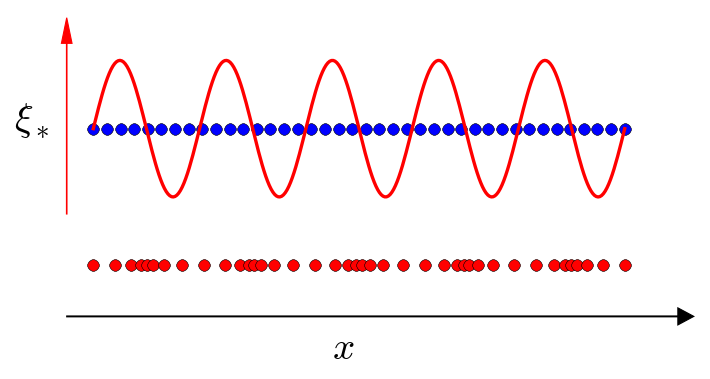
\includegraphics[width=0.7\textwidth]{Figures/1_perturbation.png}
	\caption{Schematic illustration of a sinewave density perturbation (red line) applied to an uniform distribution of matter (blue dots) and the resulting distribution (red dots). The mode displayed here has $m=10$ and its amplitude was exaggerated.} 
	\label{Fig:1_perturbation}
\end{figure}

\begin{equation} 
\label{Eq:1_FourierMode} 
   \xistar(x,0) = \xistaro \sin( kx ) ,
\end{equation}  
where the wavenumber $k$ is such that $k R_o = m \pi$ and $\xistar(R_o,0) = \xistar(R_o,\tau) = 0$ at all times. When deciding which wavenumber to choose, we must bear in mind the finite numerical resolution of the models that we will present later. The next subsection gives quantitative arguments that motivated our choices.  
The aspect of the perturbed system is shown as a rough schematic on Fig~\ref{Fig:1_perturbation}.

\subsubsection{Fourier modes: resolution issues} 
\label{Ssub:1_FourierModes}
An uniform distribution of $N$ discrete mass elements cannot resolve infinitely small wavelengths, the lower limit depends on the mean separation $l_o\simeq R_o / N^{1/3}$ which gives a reference wavelength $\lambda / R_o = \lambda_\ast \ge N^{-1/3}$ for a resolved  Fourier mode. 
Since $kR_o = m\pi$, this also implies that $ m \le 2 N^{1/3}$.  

The initial amplitude $\xistaro$  of the perturbation can be tailored to the actual Poissonian fluctuations in a uniform distribution of discrete elements. The radius bounding a shell of $N$ mass elements distributed randomly will fluctuate freely between $r$, $r + \delta r$ due to stochasticity. The radius $r$ of a uniform sphere being a power-law of mass $M$, we 
find:
\begin{equation}
\frac{\delta r}{r} = \frac{1}{3}\,\frac{\delta M}{M} =  \frac{1}{3}\,\frac{\delta N}{N} = \frac{1}{3} N^{-\frac{1}{2}}
\end{equation}
 for identical mass elements. We then compute the number-averaged value $\langle \delta r/r\rangle$ by summing over  all elements from 1 to $N$ and dividing by $N-1$ to find 
\begin{equation}
\langle \frac{\delta r}{r} \rangle = \langle \xistaro\rangle = \frac{2}{3} \frac{\sqrt{N} - 1 }{N - 1} \ .
\end{equation}  

Thus the mean amplitude (in units of $R_o$) is $\langle\xistaro\rangle\simeq 1/10$ for $N=32$ which drops to $\langle\xistaro\rangle\simeq 6\times 10^{-4}$ when $N = 10^6$. We checked that the mode with the shortest wavelength $\lambda_\ast$ still resolved would have a displacement $\langle\xistaro\rangle$ initially 
smaller than $\lambda_\ast/2$ for any sensible value of $N$. This in turn implies that this mode may grow over time to reach an amplitude $\xistar(x,\tau) \simeq \lambda_\ast/2$, which is the point when orbit-crossing between shells of constant mass must occur. In other words, at this point, the overdensity transitions from linear convergence of particles to  collisional evolution (not covered by Eqs.~\ref{Eq:1_system}). The time when shell-crossing occurs can be seen as the "birth" of a clump, whether this clumps undergoes consequent two-body relaxation effects depends on its characteristics, such as density and membership, and the remaining time before the end of expansion. 

\subsection{Segregation time-scale} 
\label{Sec:Timescales} 
We already noted that $\Hub_0^{-1}$ sets a time-scale for the expansion of the system. That time should be chosen so that it matches the hydrodynamical star formation
phase of $0.5 - 1$ Myr \citep{Maschberger2011,Bate2014}. 
When $\Hub(\tau) = 0$ and the expansion is over, the stars relax to a new equilibrium driven by star-star interactions. Therefore we need to address first the 
internal dynamics in clumps in time units of $\Hub_0^{-1}$, before discussing the later phase of violent relaxation and consider the system as a whole. 
The definitions are the same, only the face values change between the two phases of evolution. 

Let us consider a clump of membership $N_\lambda$ initiated by a Fourier mode of wavelength $\lambda$. With its total density $\rho + \delrho$ given by Eq.~(\ref{Eq:1_DeltaRho}), we may write 

\begin{equation}
 \rho_g = \frac{\rho_o}{a^3(\tau)} \, \left( 1 + \frac{\delrho}{\rho} \right) \equiv  \frac{\rho_o}{a^3(\tau)} \, \rho_\ast.
 \end{equation}
 
Combining this with Eqs.~(\ref{Eq:0_tcr}), (\ref{Eq:0_trel}) and (\ref{Eq:0_ms2}) from the introduction, the mass-segregation timescale in the clump now reads:

\begin{equation}
 \tms = \frac{0.138}{6}\pi \left(\frac{3}{4\pi}\right)^{1/2} \frac{\langle m_\star\rangle}{\max\{m_\star\}} \, \frac{N_\lambda}{\ln 0.4 N_\lambda} \, (G\rho_g)^{-\frac{1}{2}}\, . \end{equation}
  
Making use of the equality 

\begin{equation}
\frac{4\pi}{3} G\rho_o = \Hub_0^2 \Estar ,
\end{equation} 
the last three relations simplify to the expression of the new dimensionless mass-segregation timescale:

\begin{equation}\label{Eqn:Taums} 
\tau_{ms} = \Hub_0 \tms = \frac{0.138}{6} \pi \, \frac{a_\lambda^{3/2}}{(\rho_\ast\Estar)^{1/2}} \, \frac{\langle m_\star\rangle}{\max\{m_\star\}} \, \frac{N_\lambda}{\ln 0.4 N_\lambda} 
\end{equation}
where $a_\lambda$ refers to the expansion factor $a(\tau)$ evaluated at time $\tau$ when $\xistar \simeq \lambda_\ast/2$. Note that our use of Eq.~(\ref{Eq:1_DeltaRho}) to compute $\rho_g$ means that the gravitational radius $r_g$ does not have its usual definition based on the gravitational energy $W$ of the system. Linking 
$\rho_g$ to $R_g$ in this way has the advantage that $R_g$ is not derived from an implied mass profile, which is (by definition) not resolved 
here. 

Clearly the segregation time depends strongly on the mass spectrum of individual clumps, on their membership $N_\lambda$, as well as the density contrast $\rho_\ast(\tau_\lambda)$. We find the density contrast from (\ref{Eq:1_FourierMode}) and (\ref{Eq:1_DeltaRho}),  

\[ \left.\frac{\delrho}{\rho}\right|_{\tau=0} \!\!\!\! = - \frac{1}{x^2}\frac{\partial}{\partial x^2} x^2\xi = - \left( 2 \frac{\sin\, m\pi x_\ast }{m\pi x_\ast} + \cos\,m\pi x_\ast \right) m\pi   \xistaro
\]
which admits an upper-bound of $3 m\pi \xistaro$. In the course of evolution, the initial amplitude of perturbation grows to $\xistar = \lambda_\ast/2$ so that the density contrast peaks at 

\begin{equation} \label{Eqn:Densitypeak} 
  \rho_\ast = 1 + \frac{\delrho}{\rho} = 1 + 3 m\pi \lambda_\ast / 2 = 1 + 3\pi\, ,
\end{equation}
where the last substitution follows from the definition of the integer $m$. The mass $M_\lambda$ in a shell bounded by $r, r+ \lambda$, is known from the unperturbed density profile~; in terms of the total system mass ${\cal M}$, we find 

\begin{equation} \label{Eqn:Clumpmass} 
   \frac{M_\lambda}{{\cal M} } = ( \overline{3 x_\ast^2} + \lambda_\ast^2/4 ) \lambda_\ast = ( 1 + \lambda_\ast^2/4) \lambda_\ast \, , 
\end{equation}
where we have replaced $3x_\ast^2$ by its space-averaged value in  the last step.  Eq. (\ref{Eqn:Clumpmass}) provides an estimate of  bound mass of a clump formed through the growth of a radial perturbation mode. If all the stars have equal mass, or, if the stellar mass function is symmetric with respect to the mean value $\langle m_\ast\rangle$, the ratio of the number $N_\lambda$ of stars in the clump to the total number $N$ is in the same proportion as $\frac{M_\lambda}{\cal M}$. We find an estimate for $N_\lambda$ which reads 

\begin{equation} \label{Eqn:Clumpn} 
   N_\lambda = N \left( 1 + \frac{\lambda_\ast^2}{4} \right) \lambda_* .
\end{equation} 

We argued in \S2.3.2 that a resolved mode should have $\lambda_\ast \ge N^{-1/3}$, which translates as: 

\begin{equation} \label{Eqn:Clumpn} 
   N_\lambda > N^{2/3}\left( 1 + \frac{N^{-2/3}}{4} \right) .
\end{equation}
This number inserted into Eq.(\ref{Eqn:Taums}) leads to a rough picture of the segregation process in clumps. The rate of mass segregation leans  on the choice of initial value for the expansion phase, $\Hub_0$. In the limit when $\Hub_0 = 0$, there is no expansion whatsoever, and the clumps form unsegregated (aside from random associations when attributing positions and velocities to the stars) during global infall. If by contrast, the expansion is vigourous, $a_\lambda \gg 1$, and the segregation timescale remains large. For $N \sim 10^4$, we compute from (\ref{Eqn:Clumpn}) $N_\lambda \gtrsim 464$: a clump with that many stars will mass-segregate rapidly only if its stellar mass function includes very massive stars. We note that one-dimensional (radial) modes would in fact split into several smaller fragments in a three-dimensional calculation.\footnote{ A full-grown radial mode forms a thin shell subject to fragmentation. See \textit{e.g.}  \cite{Ehlerova1997,Wunsch2010}.} We expect  the clumps to form quickly  and contain $N_\lambda \ll 464$ stars, so  that the internal dynamics 
will drive mass segregation {\it before} the system expansion stops. Because this depends in the details on $\Hub_0$ and other important parameters, 
% on the clump stellar mass function, the density contrast reached, and the initial expansion rate, among important parameters, 
we defer the analysis to \S \ref{TODO} and N-body simulations. 
% Still, this simple one-dimensional mode analysis helps to understand the basics of the fragmentation proces



\subsection{Example with N = 15000} 
\label{Sec:HubbleExpansion}
%This section discusses the growth of fragments and their properties at the end of the Hubble expansion phase. Because hydrodynamical calculations of supersonic turbulence show proto-stars forming during a single free-fall time,  
%
%\begin{equation} \label{Eqn:Freefall} 
%   t_{ff} = \left(\frac{3\pi}{32 G\rho_o} \right)^{1/2} \sim 0.5 - 1 {\rm Myr}
%\end{equation}
%(where $\rho_o$ is taken as the global mean density), we should pick a set of parameters such that the clumps form over a physical time to match that of Eq.~(\ref{Eqn:Freefall}). In this work, we choose to evolve the models until $H = 0$ to allow for fully-developed individual clumps. More precisely, we look for a computational setup such that $\Hub(\tau) = 0$ in a minimum of one star-formation timescale $t_{ff}$. We do so although the approach taken here to form clumps would allow to stop the calculation {\it before} $H = 0 $ and {\it subtract} the residual radial velocities using Eqs \ref{Eq:1_HubbleExpr}. As a result, the configuration would be less fragmented than for the case when $H =0$. Thereafter the dynamical evolution would proceed similarly in all the cases, but with different clump mass- and size distributions. The choice of initial Hubble parameter $\Hub_0$ must always yield $E < 0$ in (\ref{Eq:1_Estar}) . Note again that when $\Hub_0$ is set equal to zero, we recover the classic configuration for the cold collapse of uniform bodies.




 \begin{figure}
\center
    \centering
    \begin{subfigure}[b]{0.49\textwidth}
    	\centering
    	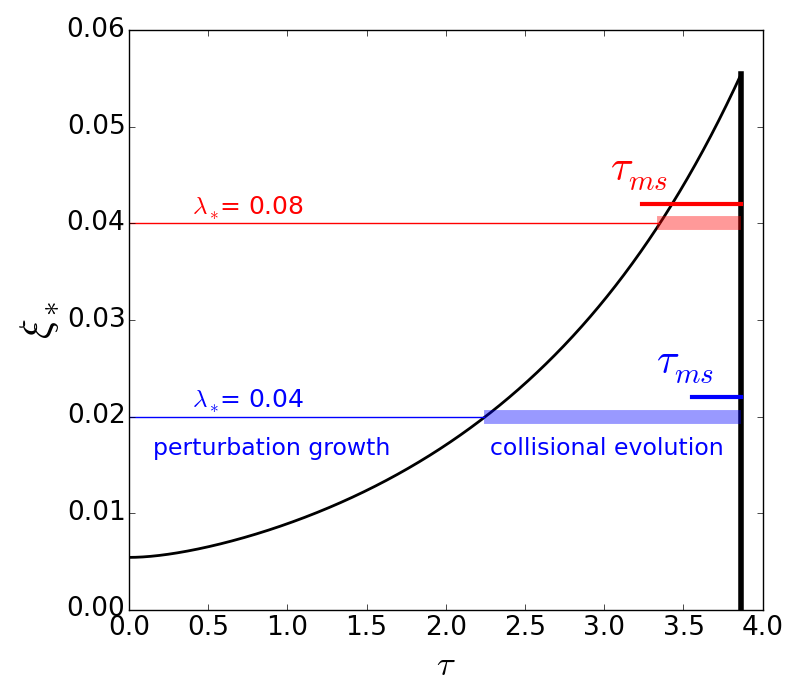
\includegraphics[width=\textwidth]{Figures/1_tau_ms.png}
        \caption{Regimes of overdensity evolution}
        \label{Fig:1_tau_ms}
    \end{subfigure}
    \begin{subfigure}[b]{0.49\textwidth}
    	\centering
    	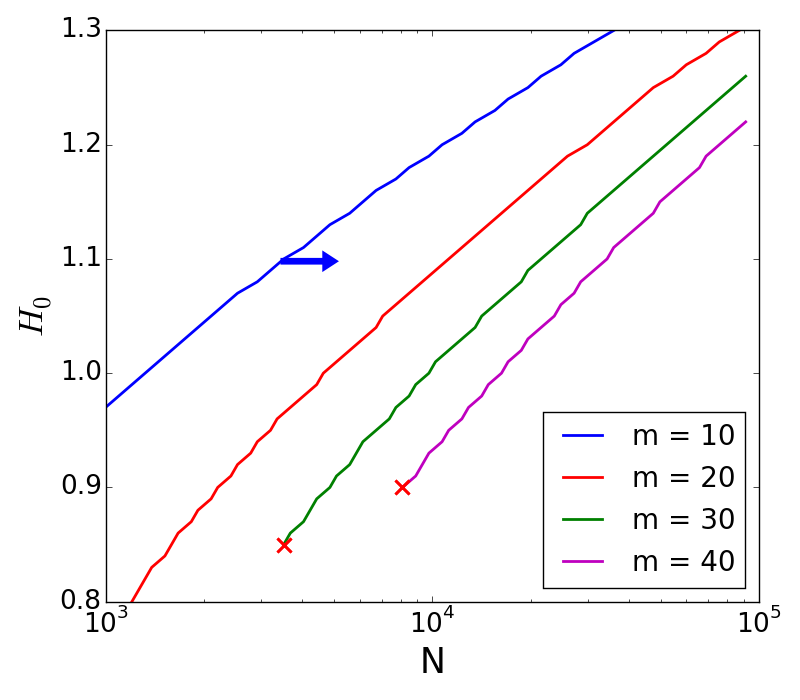
\includegraphics[width=\textwidth]{Figures/1_segregation_zone.png}
        \caption{Segregation domains}
        \label{Fig:1_segregation_zone}
    \end{subfigure}
\caption{(a): growth of perturbation $\xi_*$ over dimensionless time $\tau$ until the end of expansion at $\tau = 3.84$. An overdensity seeded with a wavelength $\lambda_*$ begins its collisional evolution when $\xi_*$ reaches $\frac{\lambda_*}{2}$. These regimes are illustrated for $\lambda_* =0.04$ and  $\lambda_* =0.08$. The overdensities have to evolve collisionally for at least $\tau_{ms}$ to mass-segregate. This time-scale is also shown for each case. The blue case evolve collisionally for several $\tau_{ms}$ and will end up mass-segregated, while the red case visibly don't have have time to segregate. Modes of large wavelength tend to produce less mass-segregated clumps. (b) for a given number of nodes $m$, a model on the right of the corresponding line (arrow for $m=10$) will have mass-segregated overdensities at the end of the expansion, will on the left, the collisional evolution is too short for segregation to sets in. The red crosses show the minimum N below which the modes cannot be resolved.} 
\label{Fig:0_perturbation_growth}
\end{figure}


We now make use of all previous development to follow the evolution of a perturbation in a given system and assess its dynamical state.

To ease comparisons with N-body calculations cast in standard H\'enon units, we set ${\cal M} = G = R_o = 1 $ and use $\Hub_0 = 1.0833 .. \simeq 1$ so that the total binding energy $E = -1/4$. The Hubble expansion proceeds until a time $t = \tau / \Hub_0 \simeq 3.87 / \Hub_0$, when $H = 0$ and the bounding radius $R$ reaches $R = a(\tau)R_o \simeq 2.4 R_o$. The evolution time up to that point coincides almost exactly with the {\it current} global system free-fall time of $\approx 4.1$ time units. System-wide collapse to the barycentre will ensue on the same time-scale, but now this process will involve the merging / scattering of several high-density clumps. 

The mass of individual stars follow a  truncated \cite{Salpeter1955} distribution function, where the distribution function $ dN/dm \propto m_\star^{-\alpha}$ with index $\alpha = 2.35$ for masses in the range  $0.3 M_\odot < m_\star < 100 M_\odot$ giving a mean value of $\simeq 1 M_\odot$. We chose this form mainly for simplicity, and for ease of calculations. 


Let us fix $\Estar = 6/7$, with $\Hub_0 = 1$ and set $N = 15 000$ as reference\footnote{The more accurate value is $\Hub_0 = 1 + 1/12 = 1.0833$ but we rounded up to 1 to simplify the discussion}. We compute a mean initial amplitude of perturbation $\xistaro \approx 0.005 $ with a shortest-resolved wavelength $\lambda_\ast \approx 0.04$. Fig.~\ref{Fig:1_tau_ms} displays the solution from integrating Eqs.~(\ref{Eq:1_system}). The amplitude $\xistar(\tau)$ grows monotonically and crosses the values $\lambda_\ast/2$ at $\tau \approx 2.3$~: thereafter the perturbation enters a non-linear regime of evolution during which the internal dynamics may become collisional $( \Delta\tau > \delta\tau_{ms})$. A second case is depicted on Fig.~\ref{Fig:1_tau_ms}, where the wavelength $\lambda_\ast = 0.08$ and the perturbation reaches amplitude $\xistar = \lambda_\ast/2$ at $\tau \approx 3.6$: there is then too little time left before the end of the Hubble expansion phase for a clump of stars to evolve collisionally ($\Delta\tau < \delta\tau_{ms}$). 





The dynamical state of individual clumps is clearly a question of membership $N_\lambda$ and mass spectrum as shown in (\ref{Eqn:Taums}). We have been arguing that most small-size clumps will show collisional internal evolution~: a small cluster of stars would lose low-mass stars in the process and so have an increased ratio of average-    to maximum stellar mass. It is not clear, then, whether this trend is strong enough to compensate for the (almost) linear dependence on membership. 
%Anticipating the results of the next section, we take $N_\lambda$ from Eq.~(\ref{Eqn:Clumpn}) to compute  a product  $N_\lambda / \ln 0.4 N_\lambda \times \langle m_\ast\rangle / \max(m_\ast) \sim 14 $ for the case of a Salpeter mass function truncated at $20 M_\odot$ ;  and about $3$ for a truncation value of $100 M_\odot$. In practice, the results of N-body 
%calculations yielded values scattered in the range [3, 14] $M_\odot$, 
%consistent with there being {\it no trend}  with clump membership $N_\lambda$. To inspect further the actual properties of clumps, we next turn to  N-body calculations. 






\section{N-body simulations}

After the previous analytical study, we present here the characteristics of actual, numerically obtained, Hubble-Lema\^itre fragmented models. The integration was performed with NBODY6, which treats the gravitational forces of stars with no softening of the potential. An example of the evolution of the system is shown on Fig~\ref{Fig:1_fragmentation}. 



\begin{figure}
\begin{center}
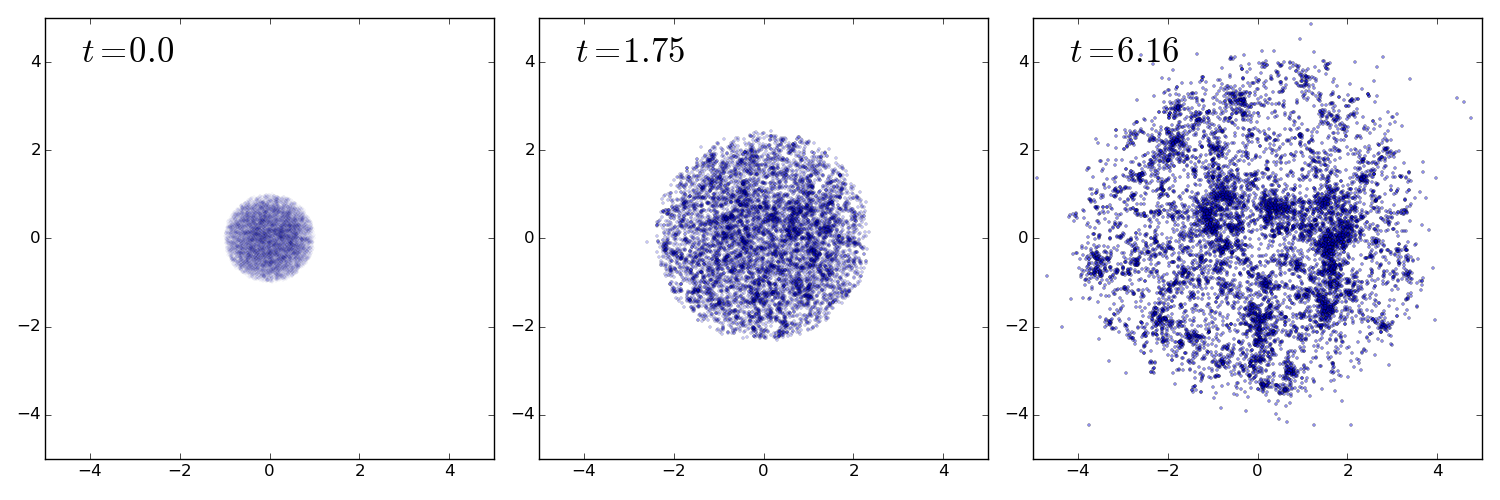
\includegraphics[width=\textwidth]{Figures/1_fragmentation}
\caption{Progressive fragmentation through the Hubble expansion. The left panel shows the initial uniform sphere; the middle panel, an intermediate step, slightly fragmented with a slowed down expansion; the right panel is the final stage, when the expansion has stopped and the fragmentation is fully developed. N=10000 particles were used in this N-body model, with $\Hub_0 = 1.0$. Time and coordinates are in H\'enon units.}
\label{Fig:1_fragmentation}
\end{center}
\end{figure}

%\subsection{Presentation of the runs}
%
%We draw $N$ stars from an Salpeter distribution function which we truncate by default to $100 M_\odot$~; in some calculations we will  use a lower bound of $20 M_\odot$, and in others we use identical masses. The code preserves the total energy and angular momentum to better than one part in $10^4$ for integration over $\sim 100 $ time units. The numerical integration starts with the expansion phase, but we will refer to the time at which this initial expansion stops ($H = 0$) as $t=0$, as we consider this dynamical state as initial conditions for cluster evolution. Memberships of 15000,40000 and 80000 were used, and 30 instances of each 15k model was performed to obtain statistically robust results.
%Table \ref{Tab:1_fragmentationmodels} summarises the main simulations used in this section to investigate the fragmentation of such systems.
%
%\begin{table}
%\begin{center}
%\caption{Summary of fragmentation models and their characteristics. These simulations started from an uniform sphere and were stopped when the expansion halted, at t=3 H.u . The third column shows the number of independent computations for each model.}
%\label{Tab:1_fragmentationmodels}
%\begin{tabularx}{\columnwidth}{XXlXX}
%\hline
%Name & N & Sampling & Mass range  \\
%\hline
%Rmh20 & 15000 & 30 & [0.35- 20 ]\\
%Rmh100 & 15000 & 30 & [0.3 - 100]\\
%Rmh1 & 15000 & 30 & 1.0 \\
%R40h20 & 40000 & 1 & [0.35- 20 ] \\
%R40h100 & 40000 & 1 & [0.3 - 100] \\
%R80h100 & 80000 & 1 & [0.3 - 100] \\
%\hline
%\end{tabularx}
%\end{center}
%\end{table}



\subsection{Clump finding algorithm}

As seen on Fig~\ref{Fig:1_fragmentation}, once expansion stops, the distribution is roughly spherical and visibly clumpy. By clump we mean here a local overdensity of stars. To characterize the model, is to characterize these substructures. Such analysis requires to find and isolate clumps, using an efficient clump-identification algorithm (or, {\it halo-finding} in cosmology).  Several methods are commonly used such as the HOP algorithm \citep{Eisenstein1998,Skory2010} which relies on attributing local densities to each particle and separating the clumps through density thresholds. The HOP algorithm is very robust on large cosmological data sets. However, our calculations have comparatively coarse statistics and noisy density fields. This issue, coupled with the  large number of free parameters of the HOP algorithm, makes the method less appealing. 

Instead we follow \cite{Maschberger2010} who adapted the minimum spanning tree (MST~; see e.g.\citealt{Allison2009b,Olczak2011}) technique to the detection of clumps. A spanning tree is a set of edges connecting a group of  particles but without closed loops~; the MST seeks to minimise the total length of the edges. One may then construct the MST for the whole system, and then delete all edges larger than a chosen cutting length, $d_{cut}$. The sub-sets that are still connected  are labeled as clumps. This process is illustrated in Fig \ref{Fig:1_MST}. In practice a minimum sub-set size $N_d$  is also chosen so as to avoid many small-N subgroups~: experience led us to choose  $N_d = 12$ for the minimum number of stars per clump. 

\begin{figure}
\begin{center}
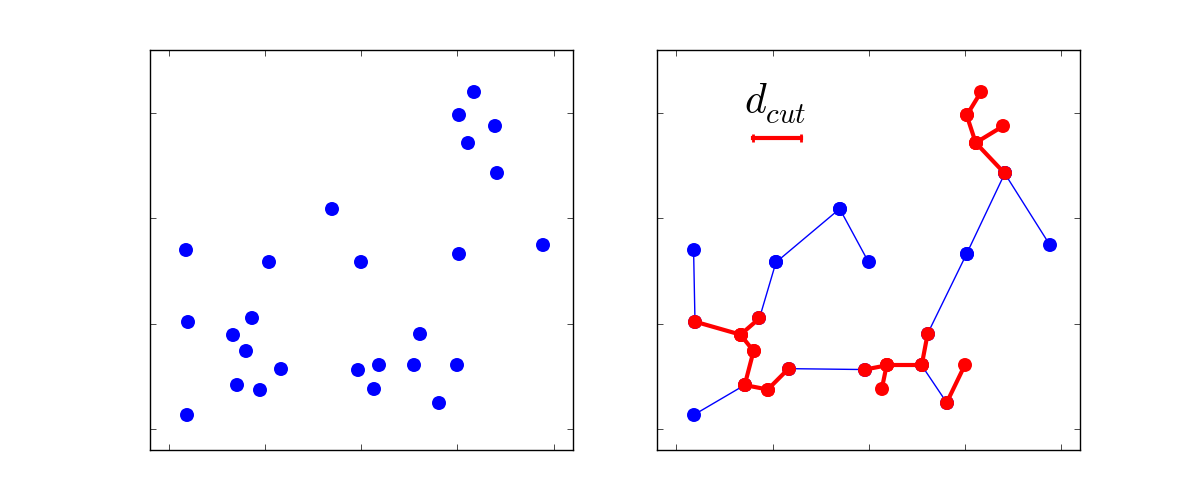
\includegraphics[width=0.8\columnwidth]{Figures/1_MST.png}
\end{center}
\caption{Illustration of a Minimum Spanning Tree and its use to isolate subgroups, using a cutting length $d_{cut}$.}
\label{Fig:1_MST}
\end{figure}


With $N_d$ fixed, the length $d_{cut}$ is then the only free parameter left. There is some freedom 
in choosing an appropriate value.
 
\cite{Maschberger2010} fixed the value of  $d_{cut}$ by visual inspection of clumps.
 We instead  identified  clumps in a fragmented system for a range of values for $d_{cut}$ and settled for the value  which optimised the number of identifications. This is shown on Fig.~\ref{Fig:1_Ndcut} for an N = 80k fully-fragmented Hubble model. For small $d_{cut}$'s, the number of detected clumps at first  increases rapidly. The rise is due  to the length $d_{cut}$ initially being small compared with the typical volume spawned by $N_d$ or more  nearest-neighbours. Beyond a certain value, a transition to another regime occurs, whereby the algorithm starts to connect previously separated clumps, counting them as one. The number of clumps thereafter begins to decrease. The value $d_{cut} \approx 0.025$ H.u optimises the outcome of the clump-search. This is a generic feature of the MST algorithm and we have adopted the same strategy throughout, adapting the value of $d_{cut}$ to the number $N$ of stars used. 

Another method to find the critical cutting length was used by \cite{Gutermuth2009,Kirk2011}. In these works, the authors build the MST, then trace the cumulative distribution function of all edges in the tree. In a clumpy configuration, there are at least two regimes: the "intra-clump" regime, with the majority of small edges, and the "inter-clump" regime with longer, scarcer edges. The intersection of a fit to these regimes provide a good cutting length for clump detection. This procedure was applied to our system and gave the same result than the clump counting, as shown on Fig~\ref{1_dcutcumulated}.

 

 
 \begin{figure}
\center
    \centering
    \begin{subfigure}[b]{0.49\textwidth}
    	\centering
    	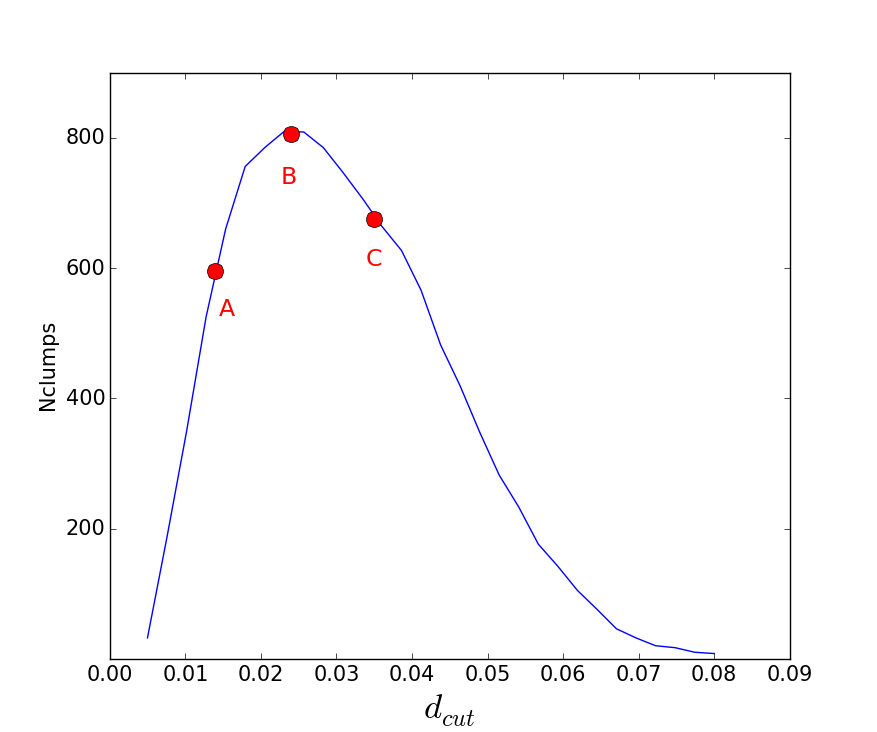
\includegraphics[width=\textwidth]{Figures/1_Ndcut.png}
        \caption{Number of clumps vs $d_{cut}$}
        \label{Fig:1_Ndcut}
    \end{subfigure}
    \begin{subfigure}[b]{0.49\textwidth}
    	\centering
    	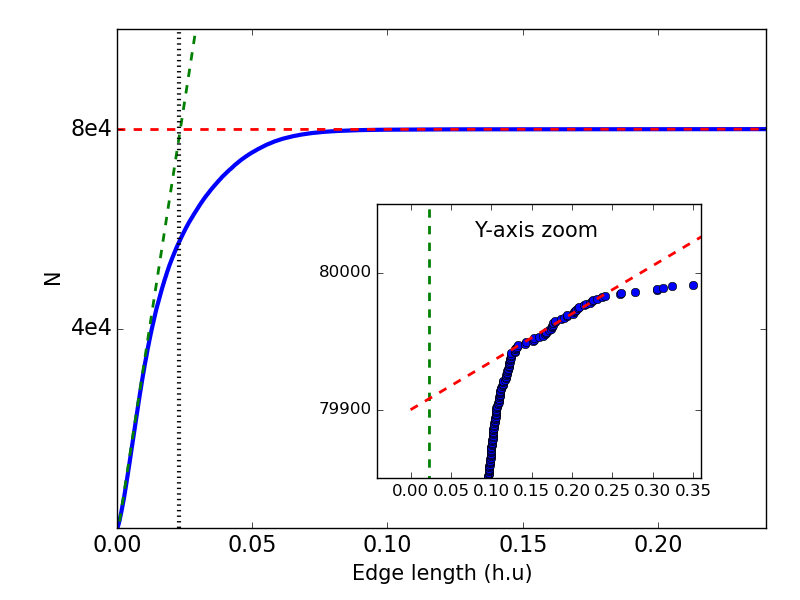
\includegraphics[width=\textwidth]{Figures/1_dcutdistribution.png}
        \caption{Cumulative distribution of MST edges}
        \label{Fig:1_dcutcumulated}
    \end{subfigure}
\caption{Two different methods to identify the critical $d_{cut}$ for clump detection. Both methods give the same value. For this 80k model, the value is 0.024 in H\'enon units. The ref linear fit on (b) was made on the linear portion with sufficient data points, discarding the very few further points departing from the tendency.}
\label{Fig:0_dcutchoice}
\end{figure}

 
   On Fig.~\ref{Fig:1_clumpsABC}, a sub-set of the model is shown where we have identified stars that belong to clumps with filled symbols. The three panels on that figure are each for a different value of $d_{cut}$, increasing from top to bottom. For the smallest value $d_{cut}$=0.015 H.u, clumps look somewhat truncated as we are still in the under-sampling regime and only their cores registered as clumps. The second, optimal, value $d_{cut}$=0.025 H.u produces visually well-isolated clumps. Finally, the third and  largest value is so that clumps begin to merge together~: this is shown by the unique clump identified in the bottom panel (filled blue squares).
   


\begin{figure}
\begin{center}
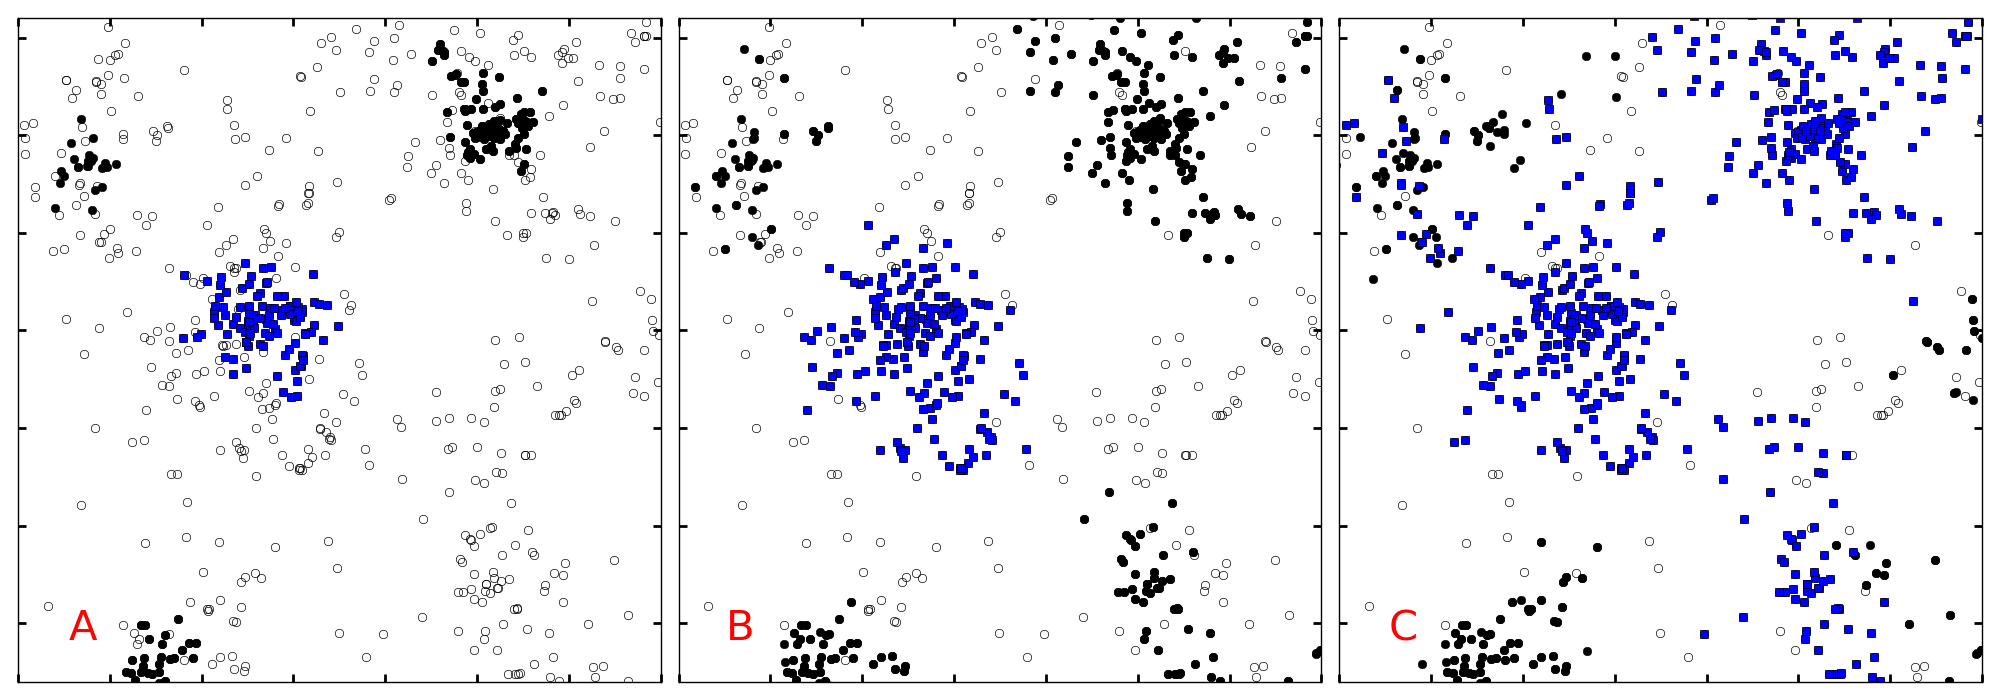
\includegraphics[width=0.9\columnwidth]{Figures/1_clumpsABC.png}
\end{center}
\caption{}
\label{Fig:1_clumpsABC}
\end{figure} 








    

\chapter{Nbody application}
\label{Chap:nbody}

After the previous analytical study, we present here the characteristics of  numerically obtained Hubble-Lema\^itre fragmented models. We present a clump-finding algorithm that we use to analyse the population of clumps obtained from the expansion. The influences of N, \tHub and stellar mass functions on the clumps mass function are investigated. We then look at the stellar content and distribution inside clumps, comparing them to clumps obtained from hydrodynamical simulations.


\minitoc



\begin{figure}
\begin{center}
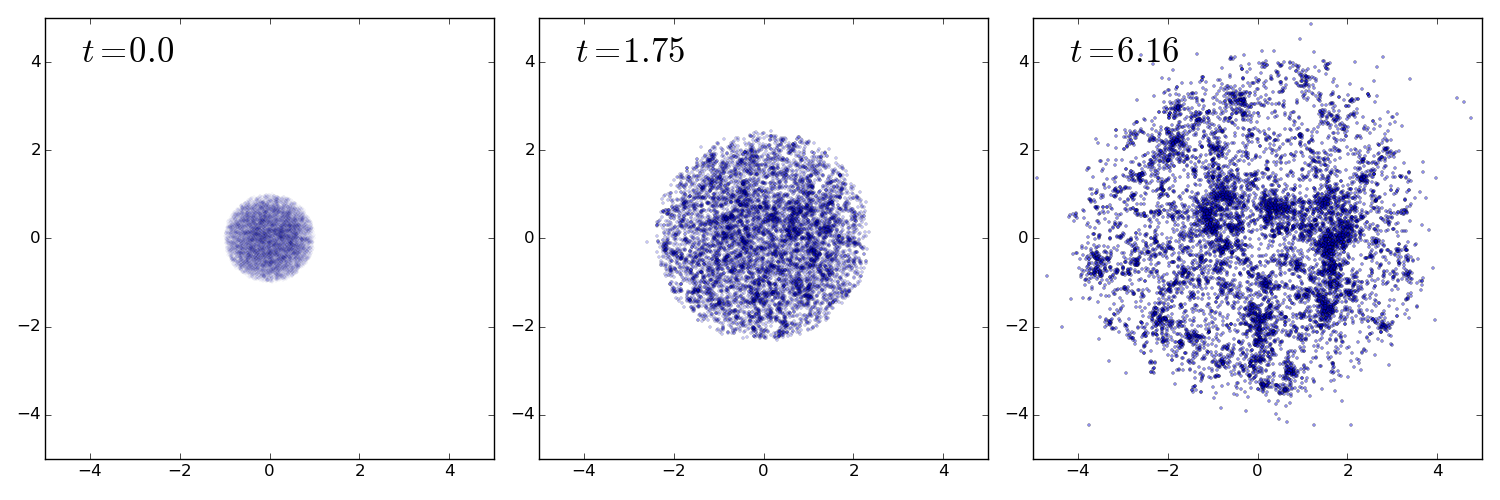
\includegraphics[width=\textwidth]{Figures/2_fragmentation}
\caption{Progressive fragmentation through the Hubble expansion. The left panel shows the initial uniform sphere; the middle panel, an intermediate step, slightly fragmented with a slowed down expansion; the right panel is the final stage, when the expansion has stopped and the fragmentation is fully developed. N=10000 particles were used in this N-body model, with $\Hub_0 = 1.0$. Time and coordinates are in H\'enon units.}
\label{Fig:2_fragmentation}
\end{center}
\end{figure}

\section{N-body simulations}




\subsection{Presentation of the runs}

To investigate the influence of various parameter and to follow the dynamical evolution (see next chapter), a large set of N-body simulation of \HubLem models was performed. They are summarised in table 

\begin{table}
\begin{center}
\caption{Summary of fragmentation models and their characteristics. These simulations started from an uniform sphere and were stopped when the expansion halted at the apex time, $t_a$. The third column shows the number of independent computations for each model. Models that stops at 40 H.u set the fragmented system as initial conditons, shifting time by $t_a$. RunsHN are detailed in the two lower tables.}
\label{Tab:2_models}
\begin{tabularx}{0.8\textwidth}{XXXXXX}
\hline
Name & N & Sampling & Mass range & $t_{end}$ & Model \\
\hline
RunsHN & see below & 175 & [0.3 - 100] & $t_a$ & Hubble \\
Rmh20 & 15000 & 30 & [0.35- 20 ] & $t_a$ & Hubble\\
Rmh100 & 15000 & 30 & [0.3 - 100] & $t_a$ & Hubble\\
Rmh1 & 15000 & 60 & 1.0  & $t_a$ & Hubble \\
R40h20 & 40000 & 1 & [0.35- 20 ] & $t_a$ & Hubble \\
R40h100 & 40000 & 1 & [0.3 - 100]& $t_a$ & Hubble \\
R80h100 & 80000 & 1 & [0.3 - 100] & $t_a$ & Hubble\\
Rh100 & 15000 & 1 & [0.3 - 100] & 40 H.u & Hubble \\
Rh20 & 15000 & 1 & [0.35- 20 ] & 40 H.u & Hubble\\
Ru100 & 15000 & 1 & [0.3 - 100]& 40 H.u & Uniform\\
Ru20 & 15000 & 1 & [0.35- 20 ] & 40 H.u & Uniform\\
\hline
\end{tabularx}
\end{center}
\subcaption*{Detailed characteristics of RunsHN:}
\begin{center}
\begin{tabular}{l|rrrrr}
\centering
N   & 1000 & 2000 & 4000 & 8000 & 16000\\ 
\hline
Sampling & 12 & 8 & 5 & 5 & 5\\
\end{tabular}
\end{center}
%Each one of these models were performed with 5 different $\Hub_0$:
\subcaption*{ Each RunsHN model is performed with 5 different \tHub.}
\begin{center}
\begin{tabular}{l|rrrrr}
$\Hub_0$ & 0.8 & 0.9 & 1.0 & 1.1 & 1.2
\end{tabular}
\end{center}
\end{table}






We draw $N$ stars from an Salpeter distribution function which we truncate by default to $100 M_\odot$~; in some calculations we will  use a lower bound of $20 M_\odot$, and in others we use identical masses. The integration was performed with NBODY6.  

An example of the evolution of the system is shown on Fig~\ref{Fig:2_fragmentation}. 





\subsection{Clump finding algorithm}

As seen on Fig~\ref{Fig:2_fragmentation}, once expansion stops, the distribution is roughly spherical and visibly clumpy. By clump we mean here a local overdensity of stars. To characterize the model, it is necessary to find and isolate clumps, using an efficient clump-identification algorithm (or, {\it halo-finding} in cosmology).  Several methods are commonly used such as the HOP algorithm \citep{Eisenstein1998,Skory2010} which relies on attributing local densities to each particle and separating the clumps through density thresholds. The HOP algorithm is very robust on large cosmological data sets. However, our calculations have comparatively coarse statistics and noisy density fields. This issue, coupled with the  large number of free parameters of the HOP algorithm, makes the method less appealing. 

Instead we follow \cite{Maschberger2010} who adapted the minimum spanning tree (MST~; see e.g. ~\citealt{Allison2009b,Olczak2011}) technique to the detection of clumps. A spanning tree is a set of edges connecting a group of  particles without closed loops~; the MST seeks to minimise the total length of the edges. One may then construct the MST for the whole system, and then delete all edges larger than a chosen cutting length, $d_{cut}$. The sub-sets that are still connected  are labeled as clumps. This process is illustrated in Fig \ref{Fig:2_MST}. In practice a minimum sub-set size $N_d$  is also chosen so as to avoid many small-N subgroups~: experience led us to choose  $N_d = 12$ for the minimum number of stars per clump. 

\begin{figure}
\begin{center}
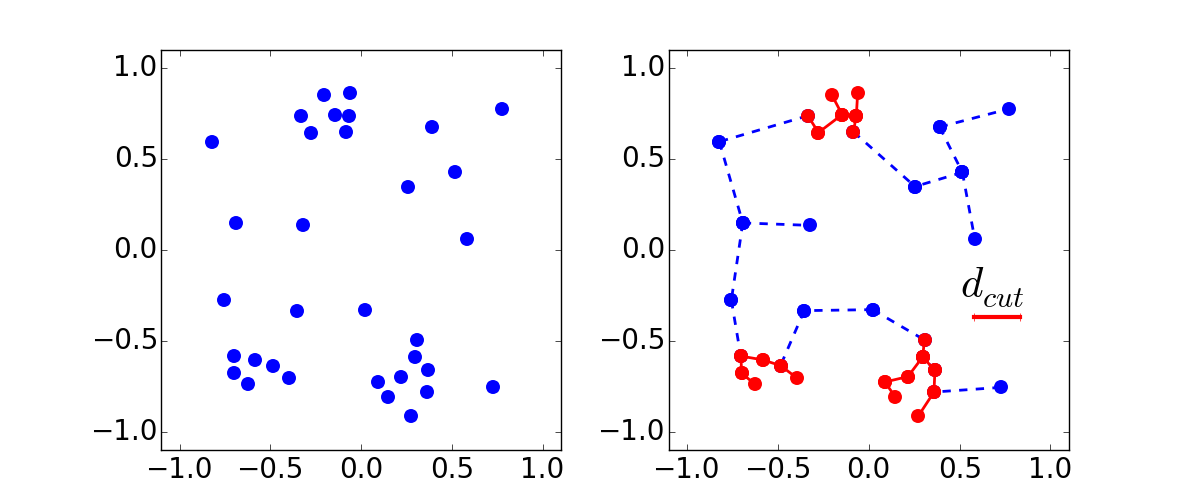
\includegraphics[width=0.8\columnwidth]{Figures/2_MST.png}
\end{center}
\caption{Illustration of a Minimum Spanning Tree and its use to isolate subgroups, using a cutting length $d_{cut}$.}
\label{Fig:2_MST}
\end{figure}


With $N_d$ fixed, the length $d_{cut}$ is then the only free parameter left. There is some freedom 
in choosing an appropriate value. \cite{Maschberger2010} fixed the value of  $d_{cut}$ by visual inspection of clumps.  We instead  identified  clumps in a fragmented system for a range of values for $d_{cut}$ and settled for the value  which optimised the number of identifications. This is shown on Fig.~\ref{Fig:2_Ndcut} for the fully-fragmented state of R80h100 (see table \ref{Tab:2_models}. For small values of $d_{cut}$, the number of detected clumps at first  increases rapidly. The rise is due  to the length $d_{cut}$ initially being small compared with the typical volume spawned by $N_d$ or more  nearest-neighbours. Beyond a certain value, a transition to another regime occurs, whereby the algorithm starts to connect previously separated clumps, counting them as one. The number of clumps thereafter begins to decrease. The value $d_{cut} \approx 0.023$ H.u optimises the outcome of the clump-search. This is a generic feature of the MST algorithm and we have adopted the same strategy throughout, adapting the value of $d_{cut}$ to the number $N$ of stars used. 


 \begin{figure}
\center
    \centering
    \begin{subfigure}[b]{0.49\textwidth}
    	\centering
    	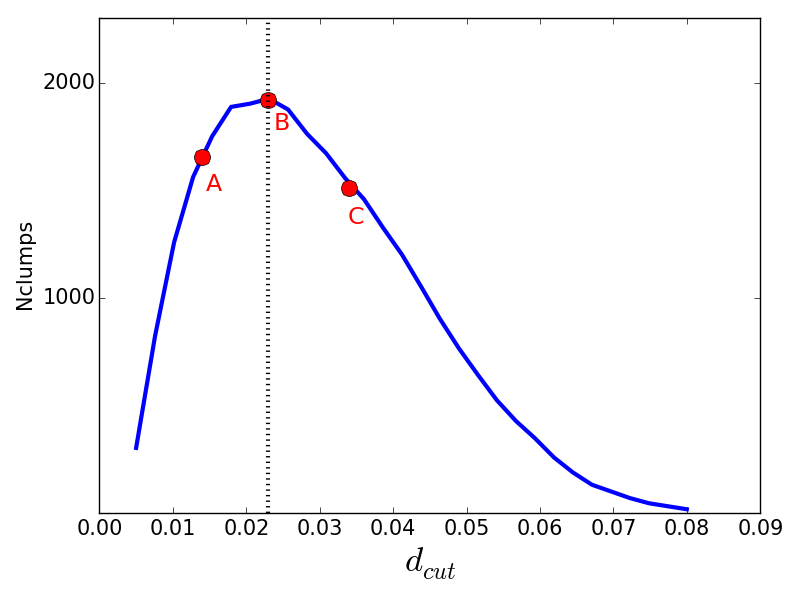
\includegraphics[width=\textwidth]{Figures/2_Ndcut.png}
        \caption{Number of clumps vs $d_{cut}$}
        \label{Fig:2_Ndcut}
    \end{subfigure}
    \begin{subfigure}[b]{0.49\textwidth}
    	\centering
    	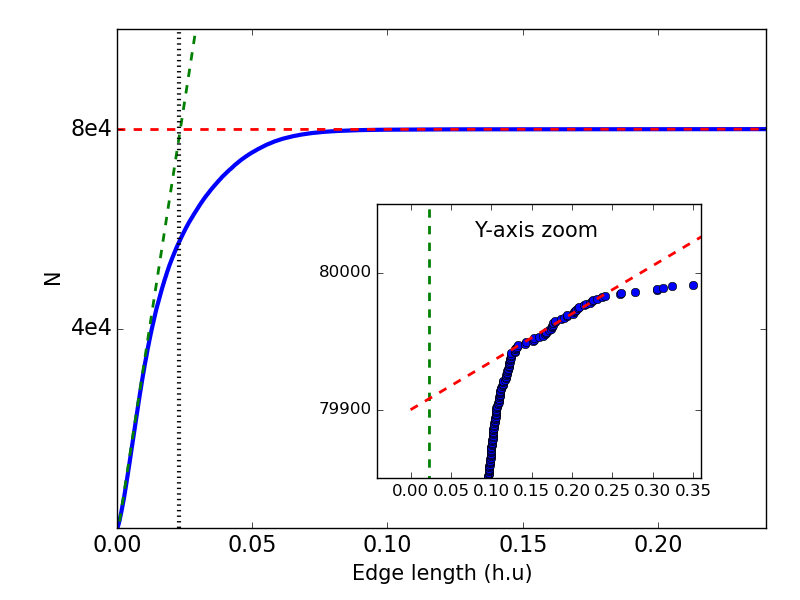
\includegraphics[width=\textwidth]{Figures/2_dcutdistribution.png}
        \caption{Cumulative distribution of MST edges}
        \label{Fig:2_dcutcumulated}
    \end{subfigure}
\caption{Two different methods to identify the critical $d_{cut}$ for clump detection. Both methods give the same value. For this 80k model, the value is 0.023 in H\'enon units. The red linear fit on (b) was made on the linear portion with sufficient data points, discarding the very few further points departing from the tendency.}
\label{Fig:0_dcutchoice}
\end{figure}


 

 


\begin{figure}
\begin{center}
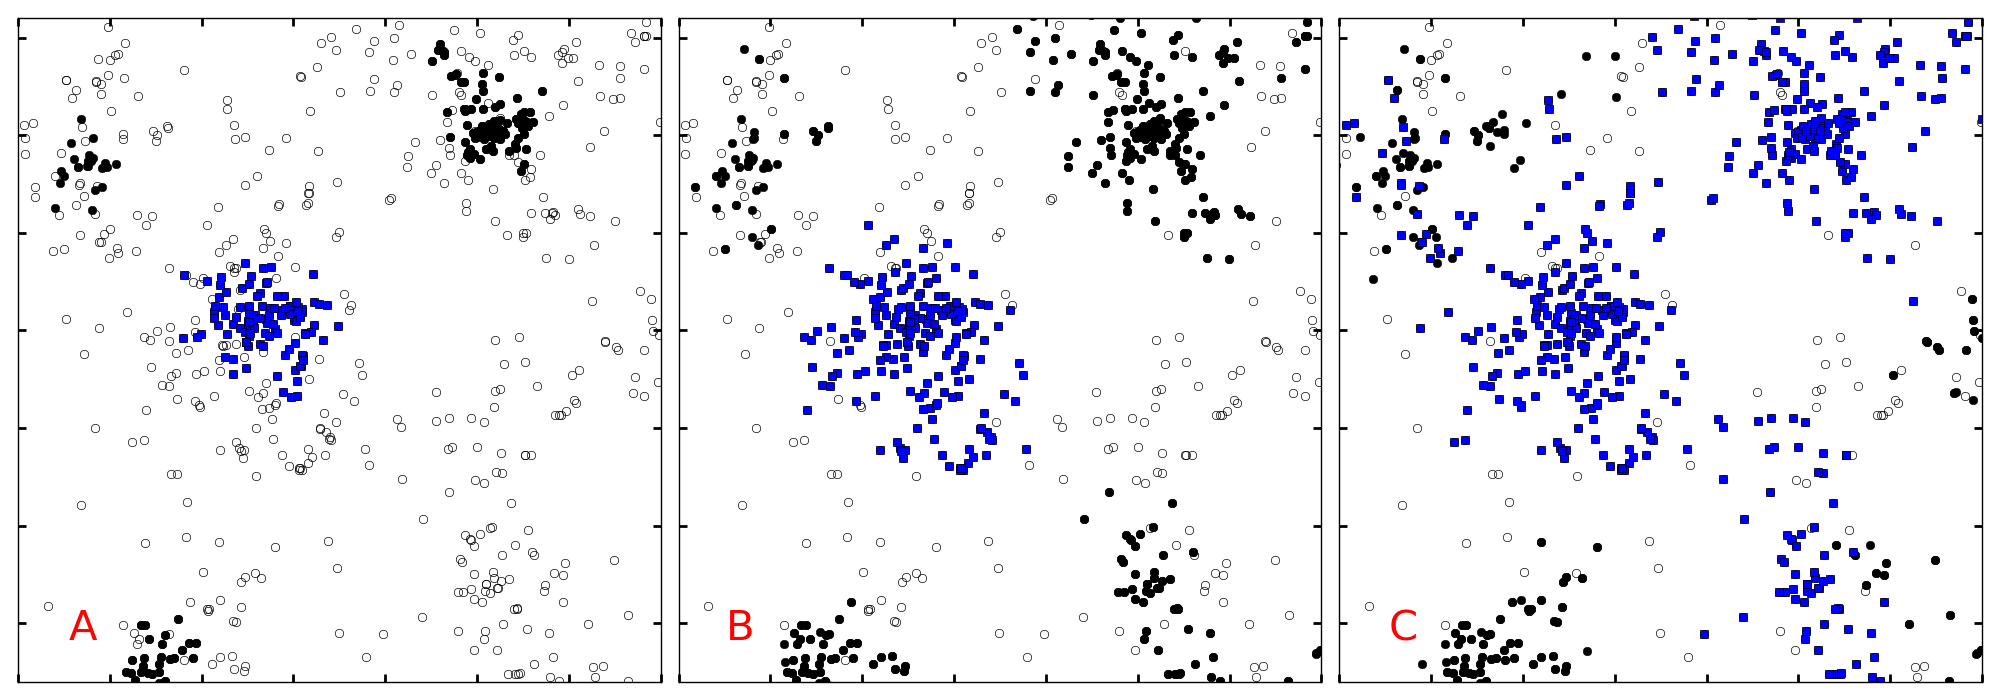
\includegraphics[width=\columnwidth]{Figures/2_clumpsABC.png}
\end{center}
\caption{Example of detected clumps for three cutting length, 0.014 (top panel), 0.024 (middle panel), 0.034 (bottom panel), which were labeled A,B,C  in Fig.~\ref{Fig:2_Ndcut}. A cube within a 80k particles fragmented model was extracted and projected.  Empty circles are stars which do not belong to any clump, black circles are clump members, and blue squares are stars that are identified as a single large  clump. Tick marks are spaced by 0.05 length units for a box size of 0.35 units.}
\label{Fig:2_clumpsABC}
\end{figure} 




Another method to find the critical cutting length was used by \cite{Gutermuth2009,Kirk2011}. In these works, the authors build the MST, then trace the cumulative distribution function of all edges in the tree. In a clumpy configuration, there are at least two regimes: the "intra-clump" regime, with the majority of small edges, and the "inter-clump" regime with longer, scarcer edges. The intersection of the linear fits to these regimes provide a good cutting length for clump detection. This procedure was applied to our system and gave the same result than the clump count, as shown on Fig~\ref{Fig:2_dcutcumulated}.

 
   On Fig.~\ref{Fig:2_clumpsABC}, a sub-set of R80h100 is shown; we have identified stars that belong to clumps with filled symbols. The three panels on that figure are each for a different value of $d_{cut}$, increasing from top to bottom. For the smallest value $d_{cut}$=0.013 H.u, clumps look somewhat truncated as we are still in the under-sampling regime and only their cores registered as clumps. The second, optimal, value $d_{cut}$=0.023 H.u produces visually well-isolated clumps. Finally, the third and  largest value is so that clumps begin to merge together~: this is shown by the unique clump identified in the bottom panel (filled blue squares).
   
   
   
   
\section{Clump mass function}

The numerical realizations of the \HubLem model allows to assess the influence of important parameters on the fragmentation, such as \tHub, N and the stellar mass function. 


\subsection{Influence of H and N}

We wish to evaluate the influence of $\Hub_0$ and N on the fragmentation and clump growth. $\Hub_0$ tunes the strength of the expansion, which tunes the duration of the fragmentation. A stronger initial expansion allows for more time for clumps to grow, so we expect more massive clumps with increasing $\Hub_0$. On the other hand, a higher N smooths the spatial distribution, reducing Poisson noise in the  distribution. However, a high membership only samples more stars from the same stellar mass function, and the density fluctuations should not change in nature, just scale down with the average distance between stars.  We do not expect N to significantly affect the fragmentation in physical units. 

To verify these, a set of simulation was performed to explore the mass function of clumps in the $\Hub_0$-N parameter space. The models have 5 different memberships that go as powers of 2 in thousands, with an increasing sampling to obtain acceptable statistics. They are summarised in table \ref{Tab:2_models} under the name RunsHN.


\subsubsection*{Apex time}
In section \ref{Sec:1_apextime}, we derived an analytical prediction for the apex time of our expanding models. To compare our numerical realizations to this prediction,  we follow for each model the evolution of the half-mass radius over time, then take the apex time as the maximum radius time, when the cluster stops expanding and starts collapsing. 


\begin{figure}
\begin{center}
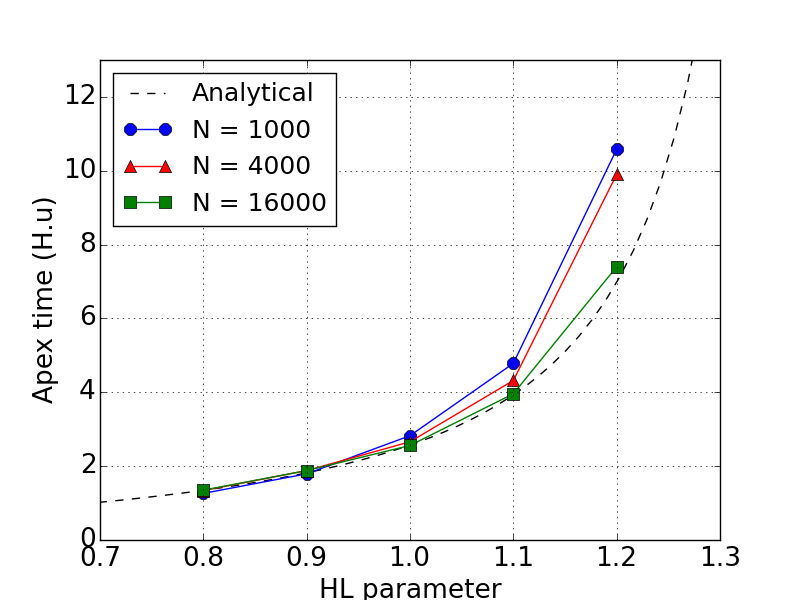
\includegraphics[width=0.6\textwidth]{Figures/2_apextime_NH.png}
\end{center}
\caption{Analytical and simulated apex times as a function of \tHub.}
\label{Fig:2_apextime_NH}
\end{figure} 

We show on Fig~\ref{Fig:2_apextime_NH} the expected analytical curve as a dashed line, then the numerically obtained apex times from our different \tHub and memberships, averaged over all similar runs. The 16k runs follow the analytical expectation within 5\%, while lower membership models take more time than expected to stop expanding at high \tHub, overshooting by as much as 30\% for \tHub =1.2. Visual inspection of the runs showed that low memberships were more susceptible to have a clump "take over" during the expansion. As we will show in the present section, low-N clusters contains more massive clumps in relative mass than high-N models. When a massive enough clump form during the expansion, it offsets the matter distribution and skews the half-mass radius (computed from the barycenter of the full system) to higher values, offsetting its fall from the collapse. To reduce unwanted "sur-fragmentation" effect, we use analytical apex times to select our fragmented configurations.  


\begin{figure}
\begin{center}
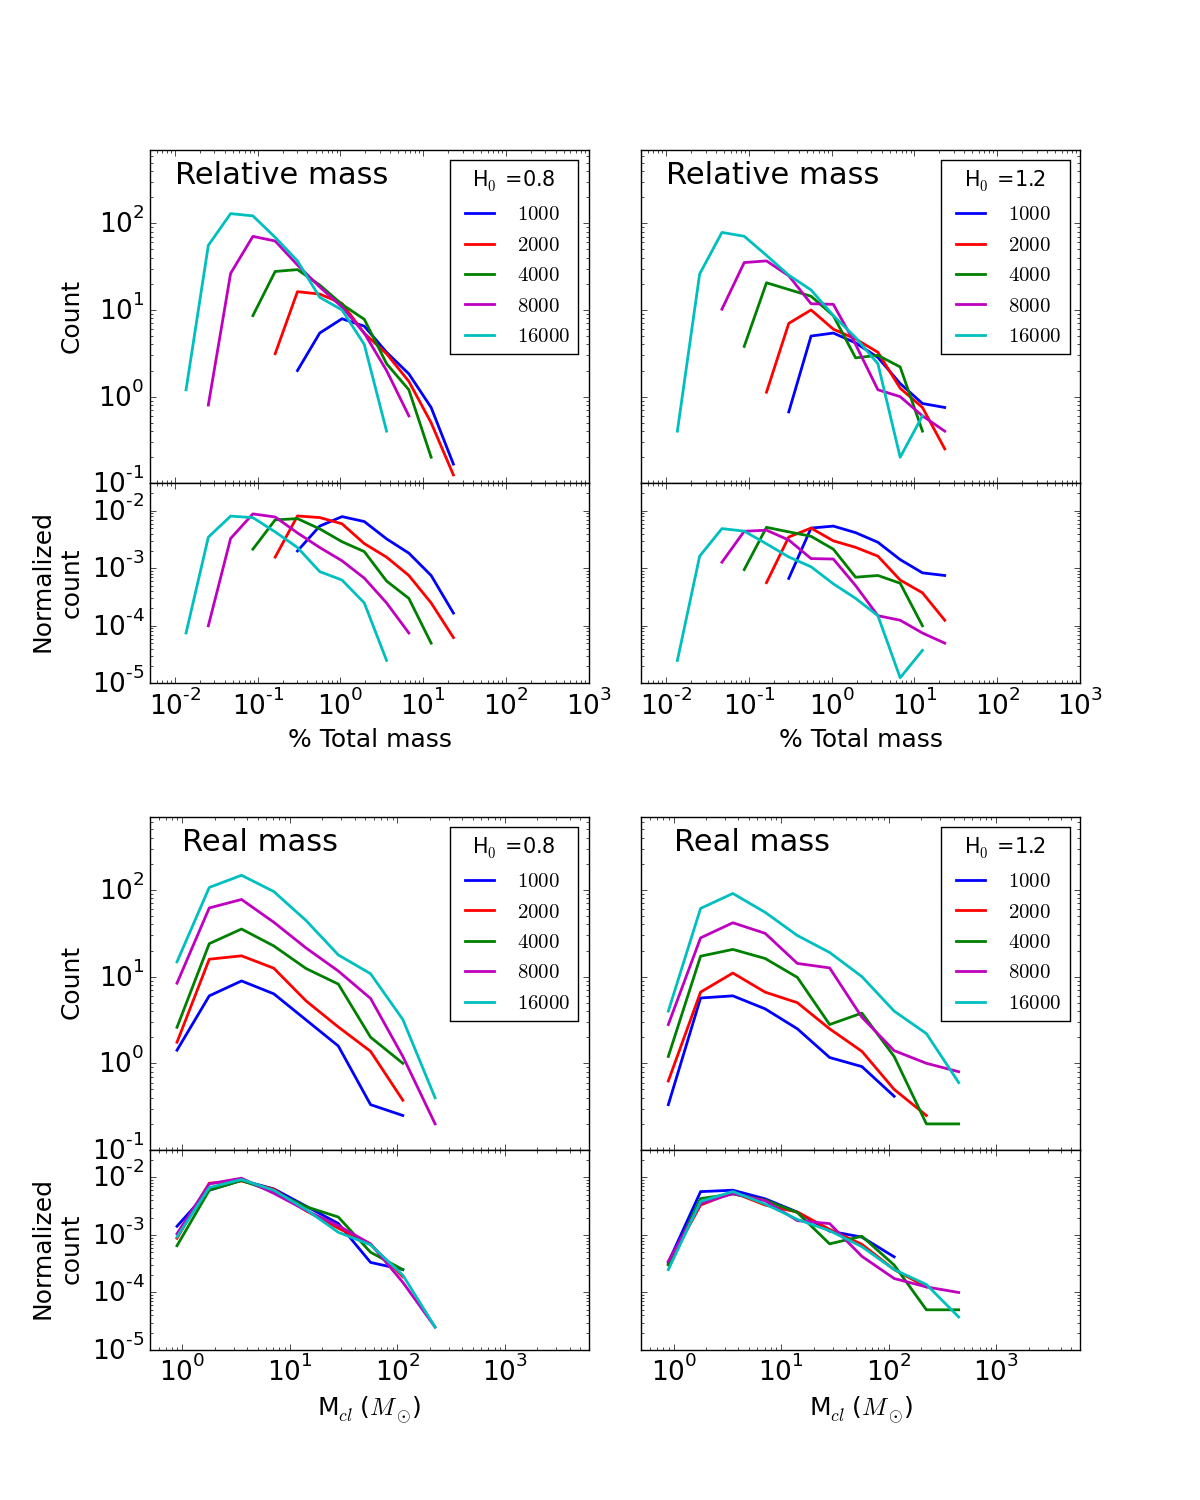
\includegraphics[width=\columnwidth]{Figures/2_ClumpMF_N.png}
\end{center}
\caption{Clump mass function for several memberships and two $\Hub_0$. Masses in the top panels are in H\'enon units, the x-axis was scaled with a factor 100 to get a percentage of the total mass of the system. Bottom panel masses are in physical units. In each panel, top sub-panel shows actual clump count in each bin (averaged over sampling), while bottom sub-panel normalize the count by the model membership. }
\label{Fig:2_ClumpMF_N}
\end{figure} 

\begin{figure}
\begin{center}
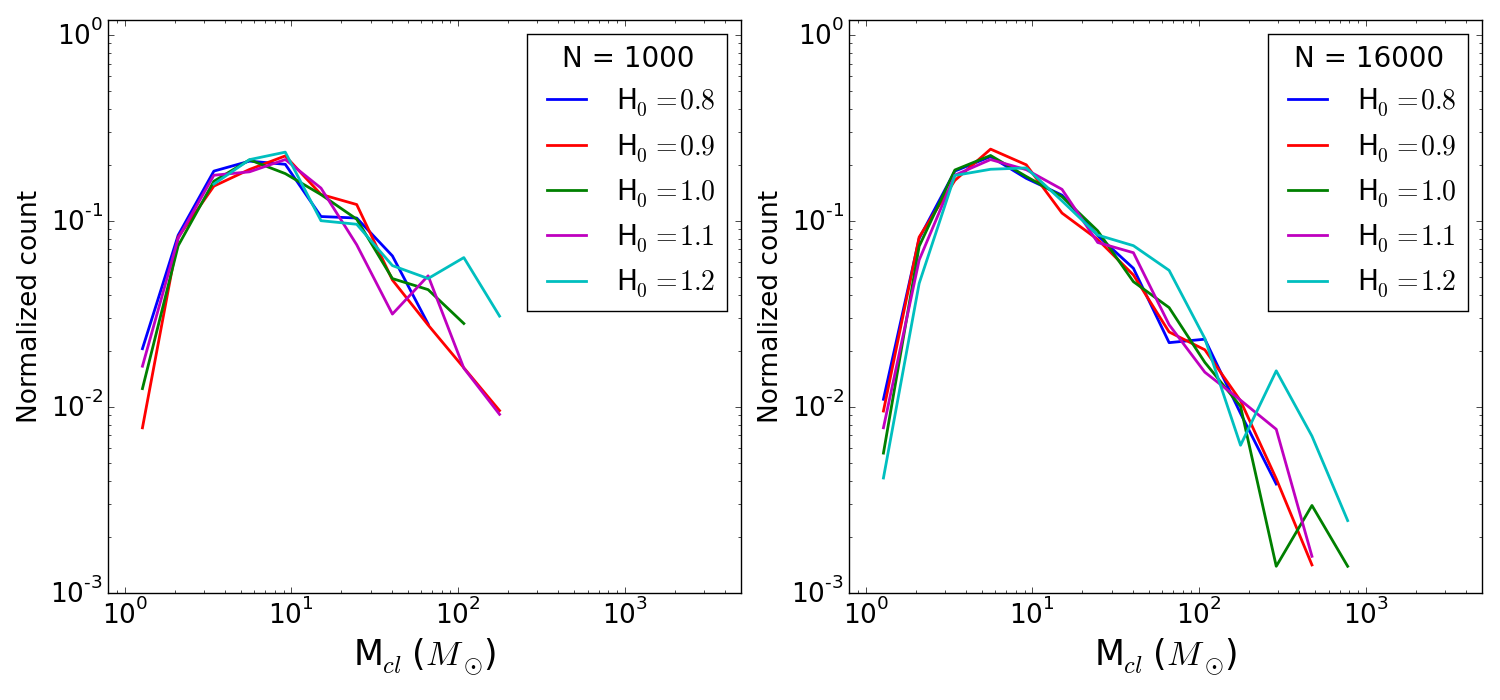
\includegraphics[width=0.95\columnwidth]{Figures/2_ClumpMF_H.png}
\end{center}
\caption{Clump mass function (real mass) for several $\Hub_0$  and two memberships.}
\label{Fig:2_ClumpMF_H}
\end{figure} 


\subsubsection*{Clump mass function}
 The clump-finding algorithm was ran on the fragmented models to obtain the clump mass function. The results are summarised as histograms on figures \ref{Fig:2_ClumpMF_N} and \ref{Fig:2_ClumpMF_H}.We have used bins of constant logarithmic intervals. We average the results over each model's sampling, hence the histogram can go down to fractional values.
 
 Looking at the top panels of Fig~\ref{Fig:2_ClumpMF_N}, we see the mass function of clumps in \textit{relative} mass, the percentage of total mass they contain.  Clumps in small-N systems tends to contain a much larger portion of the total system mass than in large-N systems, which is even clearer in the normalized count sub-panels. In fact, for \tHub = 0.8, the peak of the mass function for N=1k happens at 1.1\% of total mass, while for N=16k, it happens at 0.07\%. These values ratio gives $\sim$ 16, the membership ratio: the clumps relative masses are inversely proportional to the model's membership.
 
This can be interpreted as a underlying common clump distribution in physical mass, regardless of the total membership of the model. This is confirmed by looking at the bottom panels of Fig~\ref{Fig:2_ClumpMF_N}, in which clump distributions are plotted in physical mass, once the masses of stars have been rescaled from H\'enon units to match the original stellar mass function. Looking at the normalized count subpanels, it is clear that 1k and 16k models have the same clump distribution, when raw count subpanels show clumps are expectedly more numerous in high-N models. The difference between \tHub = 0.8 and 1.2 is not clear from the graph, but it seems a higher \tHub pushes the upper limit of the distribution to slightly higher masses.

To illustrate this last trend, we turn to Fig~\ref{Fig:2_ClumpMF_H} where clump MF are shown for various \tHub and a common membership. For  both N=1k and N=16k, the distribution preserves its shape for various \tHub, and gets prolonged at higher clump masses for N=16k, as more mass is available to build clumps.

 Thought the distribution does not undergo any dramatic change, a weak trend with \tHub is seen in both panels: as the strength of expansion increases, the distribution slightly decreases at low clump masses and slightly increases at higher clump masses, the pivot masse being $\sim$ 30 $\Mo$. We look at the 16k model and follow the cumulated mass inside all clumps, as well as the percentage of this mass in clumps below and above 30 $\Mo$, for different \tHub:

\begin{center}
\begin{tabular}{l|rrrrr}
\centering
\tHub   & 0.8 & 0.9 & 1.0 & 1.1 & 1.2\\ 
\hline
$M_{tot}$ & 3502 & 3478 & 3582 & 3683 & 3561\\
$ < 30 \Mo$(\%) & 66 & 65 & 55 & 49 & 44\\
$ > 30 \Mo$(\%) & 34 & 35 & 45 & 51 & 56\\
\end{tabular}
\end{center}

From this data, we get two facts about our fragmented models: the mass contained in clumps does not depend on \tHub ($<$2\% dispersion) and there is a transfer of mass from small clumps to more massive ones as the expansion lasts longer.

To summarise: the general shape of the clump mass function is common to all membership and \tHub. In physical mass, the same clumps form in 1k and 16k models, almost regardless of the duration of the expansion. We note a mass transfer from small to high mass clumps when \tHub increases, that is consistent with a merging process: small clumps assemble or get accreted by large clumps. When the initial expansion is strong, the merging lasts longer and more mass in transferred. This is confirmed by visual inspection of the models, as we see clumps merging during the expansion.




\subsection{Influence of stellar mass function}
\label{Sub:2_ClumpMF_MF}




Neither \tHub or N seem to heavily influence the shape of the clump mass function. We now turn to another parameter: the stellar mass function. We know the clumps are seeded by density fluctuations in the initial uniform sphere. These fluctuations are governed by pure Poisson noise in the case of identical stellar masses, but are modified and enhanced once stars follow a mass function themselves: a high-mass star surrounded by lighter ones will by itself introduce a localized strong density fluctuation. We expect a relation between the clump mass funtion and  the {\it stellar} mass function in the generated initial conditions.

We wish to quantify this relation. To this end, we ran a set of simulations where all the stars have the same mass, and two sets for which a Salpeter mass function with $\alpha = 2.35$  was truncated at different upper- and lower-bounds. A total of 15000 stars in a Hubble configuration were used, all let go  with the same initial expansion rate  $\Hub_o = 1$. For the multi-mass models, the mass range  was chosen as $[0.3, 100]\, M_\odot$ and $[0.35, 20]\, M_\odot$ so that the mean stellar mass $= 1M_\odot$ as for the single-mass models. Thirty different runs were performed in each case and the outcome averaged for better statistics. These are refered to as Rmh1, Rmh100 and Rmh20 in Table \ref{Tab:2_models}.

On Fig.~\ref{Fig:2_ClumpMF_MF}, we display the  number of clumps as function of clump mass for the truncated Salpeter  models as a red solid line, while the single stellar mass models are shown in green dash. A grey shade indicates one standard deviation where statistics allow ({\it i.e.}, large numbers), and, as in previous section, we have used bins of constant logarithmic mass intervals.  Fig.~\ref{Fig:2_ClumpMF_MF_1} shows Rmh20 models, and \ref{Fig:2_ClumpMF_MF_2} shows Rmh100 models. 
With clump membership restricted to $N \geq 12$, the identical-mass model  stays relatively close to a power law (straight dotted line on the figure) of index $\approx -4$ for the higher mass clumps. A spread in stellar masses leads to much more massive clumps (we counted $\simeq80$ clumps of $12 M_\odot$ for the equal-mass case~; and $\approx 32$ with a mass $ \le 12 M_\odot$ for the other ones) . This transforms the clump mass function, from a near-power-law, to a bell-shaped distribution.  





 \begin{figure}
\center
    \centering
    \begin{subfigure}[b]{0.49\textwidth}
    	\centering
    	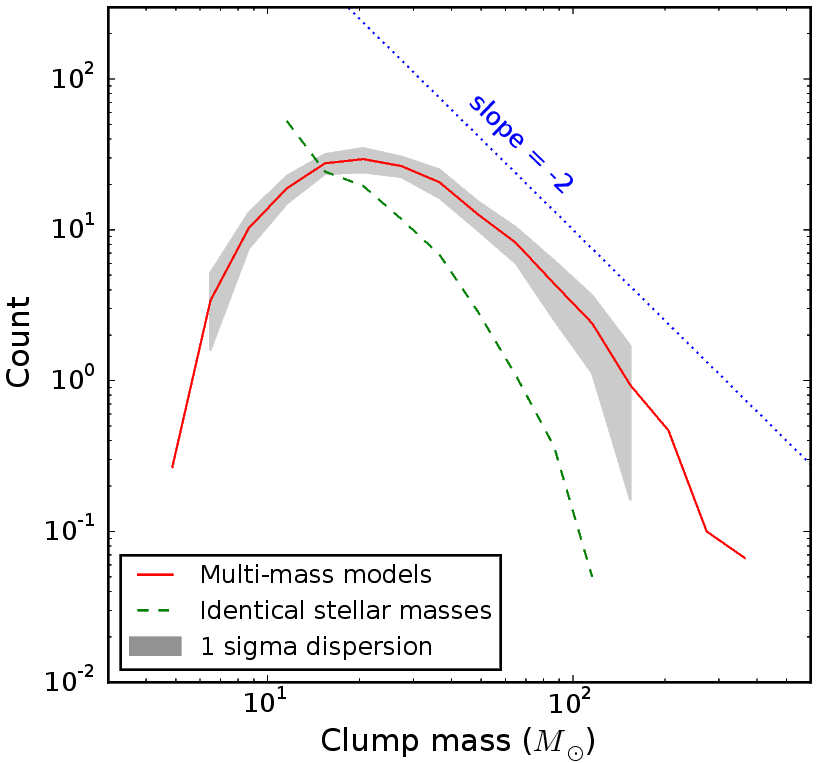
\includegraphics[width=\textwidth]{Figures/2_ClumpMF_MF_1}
        \caption{Stellar mass range $[0.35, 20]\, M_\odot$ }
        \label{Fig:2_ClumpMF_MF_1}
    \end{subfigure}
    \begin{subfigure}[b]{0.49\textwidth}
    	\centering
    	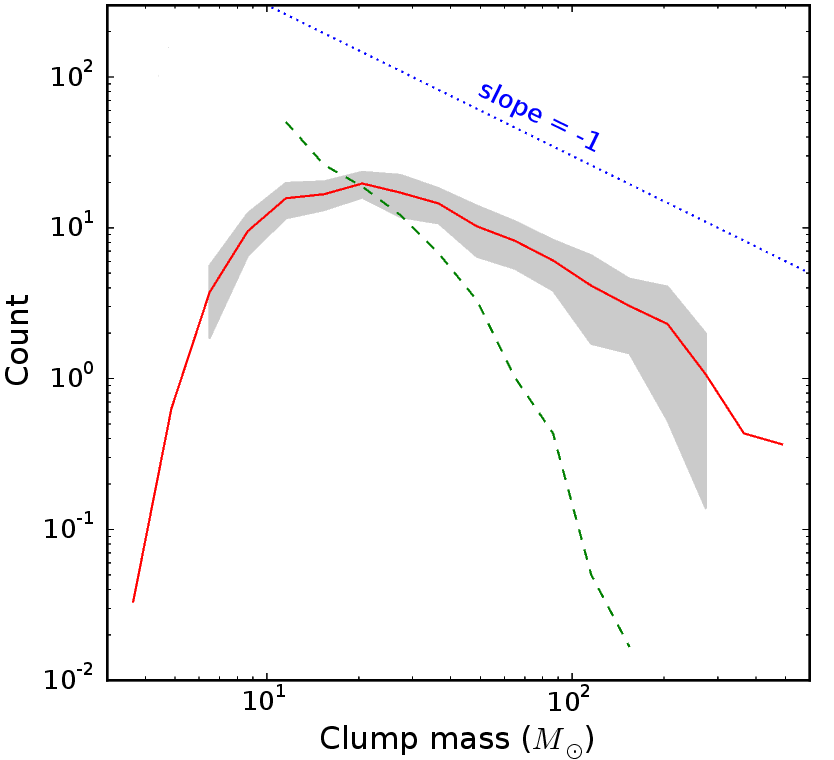
\includegraphics[width=\textwidth]{Figures/2_ClumpMF_MF_2}
        \caption{Stellar mass range $[0.3, 100]\, M_\odot$}
        \label{Fig:2_ClumpMF_MF_2}
    \end{subfigure}
\caption{Mass function of the clumps identified with the MST algorithm. The calculations all had $N = 15 000$ stars, and we have averaged over 30 realisations for each configuration.  The results for three stellar mass functions  are displayed~: a model with equal-mass stars (green dashed line)~; a Salpeter distribution function truncated at $20 M_\odot$ (solid red line, left)~; a Salpeter distribution function truncated at $100 M_\odot$(solid red line, right). (a) The clumps  mass function for equal-mass models  shows a trend with mass roughly in agreement with an $M^{-4}$ power-law. By comparison,  the results for an  Salpeter stellar distribution function  truncated at $20 M_\odot$ has a bell-shaped profile, with a peak around $M = 20.5 M_{\odot}$~; only the tail-end shows marginal agreement with an $\propto M^{-1.7}$ power-law (dotted line on the figure)~; (b) another Salpeter distribution function but with  the upper-mass truncation  set at $100 M_\odot$. The tail at large clump mass is now much flatter, with a slope $\approx M^{-1}$, (dotted line on the figure as well). The bins used  had constant logarithmic mass intervals.}
\label{Fig:2_ClumpMF_MF}
\end{figure}



When very massive stars are included in the calculations, yet more massive clumps are formed (Fig.~\ref{Fig:2_ClumpMF_MF_2}). The formation of large sub-structures depletes the number of clumps around the peak value, and so the distribution becomes broader and shallower. The mean clump mass for the different cases read $20 M_\odot$ (equal-mass), $32 M_\odot$ (Salpeter $m_{max} = 20 M_\odot$) and $45 M_\odot$ (Salpeter $m_{max} = 100 M_\odot$), a steady increase with the width of the stellar mass spectrum. On the other hand, the position of the peak of the distribution remains unchanged at (roughly) $20$ to $21M_\odot$. The trend in total number of clumps detected is a slight {\it de}crease with the broadening of the  stellar mass spectrum, from 187, down to 151 respectively for the $m_{max}=20$ and $100 M_\odot$ Salpeter models.  
%  Much of this difference in the  number of clumps is accounted in the 
 % range 0 to $20 M_\odot$, for which 73 and 54 clumps were found, respectively. 
% The fractional decrease of 26\% compares well with the lower number of stars in the interval 
% $[10,20]M_\odot$   for the model with the broader mass spectrum (which reaches $20\%$).  
  We observe that the overall fraction of  stars found in clumps (some $\approx 6500$ out of 15000, or 43\%) stays unchanged.
  
We argue that the shape of the clump mass spectrum provides indirect evidence for the role of massive stars predominantly as seeds for growth in our simulation. This is to be opposed to a full hierarchical build-up of clumps from very tiny sub-structures. There are two tell-tale signs to support this view~: a) if high-mass clumps formed through the repeated and stochastic merger of small clumps, then the clump mass function should tend to a log-normal distribution, which is  symmetric (in logarithmic scales) with respect to the peak value, whereas the distributions shown here lack this basic property~; and b) the ratio of maximum clump mass to mean mass may exceed 15 when the  stellar truncation mass is set to $20\, M_\odot$, and reaches only $\sim 4$ in the case when the upper mass is set to $100\, M_\odot$. If small-ish clumps were merging at the same rate in both models, then this ratio should be comparable. Instead, very large clumps take too long to assemble and the merger rate drops with clump mass. Recall that all fragmentation calculations ran for the same total time. There is a weak merging process happening, as shown in the previous section, but it is marginal, as heavy clumps likely form from massive star seeds.

To check this hypothesis, we borrow from black hole dynamics in galactic nuclei the notion of a {\it radius of influence}, which is the radius  enclosing as much mass in the stars as the central black hole mass (see e.g. \citealt{Merritt2013}).  Here, the stars inside the influence radius are bound to the massive star at the centre. Thus if a massive star is a seed for a clump, and only the stars inside the influence radius remain bound to it, we should count as many clumps in the mass range $2m_\star, 2 m_\star + 2{\rm d}m_\star$, as there are stars in the range $m_\star, m_\star + {\rm d}m_\star$.  The maximum clump mass exceeds twice that of the most massive stars $m_{max}$, which implies some degree of merging and is consistent with the previous section. If we count all clumps starting from the truncation value $m_{max}$ of the stellar mass function,  
%presume that the clumps all formed from fragments seeded with a massive star and its cortege of bound stars, 
then we should find as many clumps in the mass range above $m_{max}$, as there are stars in the interval $[m_{max}/2, m_{max}]$.  We find for runs with $m_{max} = 20 M_\odot$ some $120$ clumps more massive than that, when there are $\simeq 100$ stars in the range $[10, 20] M_\odot$, essentially identical~; and some $14$ clumps of $100 M_\odot$ or more, when there are (on average) 9 stars in the mass range $[50, 100] M_\odot$. This calculation suggests that  most massive stars act as seeds for the formation of large clumps in the generated initial conditions.













\section{Clump contents}

In this section we compare the clump configurations derived from the \HubLem expansion method with the distribution of proto-stars that form in hydrodynamical simulations. We first look at the velocity field inside and outside the clumps, then we investigate the stellar content of the clumps themselves and their mass segregation.


\subsection{The velocity field}
\label{sec:velocityfield} 




 \begin{figure}
\center
    \centering
    \begin{subfigure}[b]{0.49\textwidth}
    	\centering
    	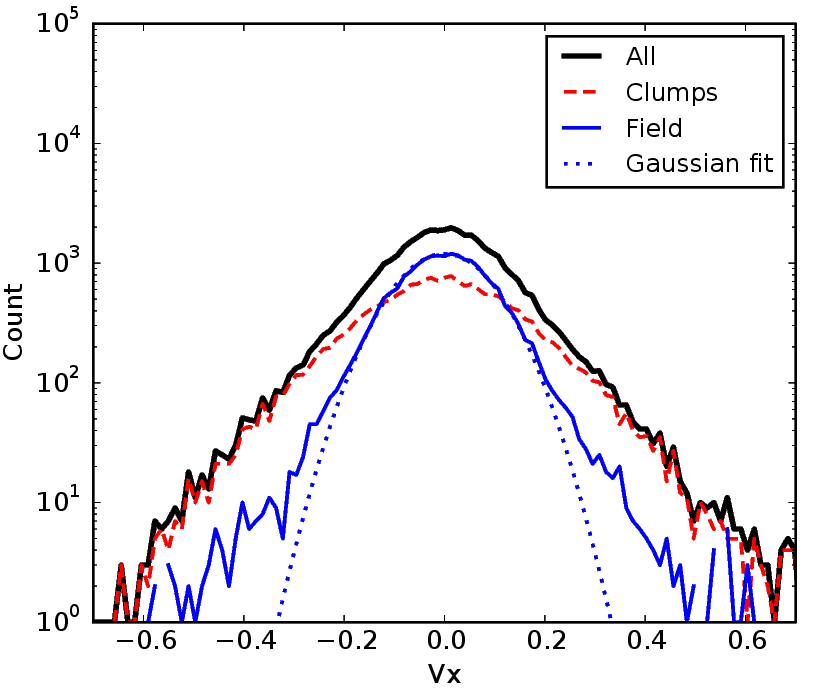
\includegraphics[width=\textwidth]{Figures/2_Vx_histogram_1}
        \caption{Distribution clumps/field}
        \label{Fig:2_Vx_histogram_1}
    \end{subfigure}
    \begin{subfigure}[b]{0.49\textwidth}
    	\centering
    	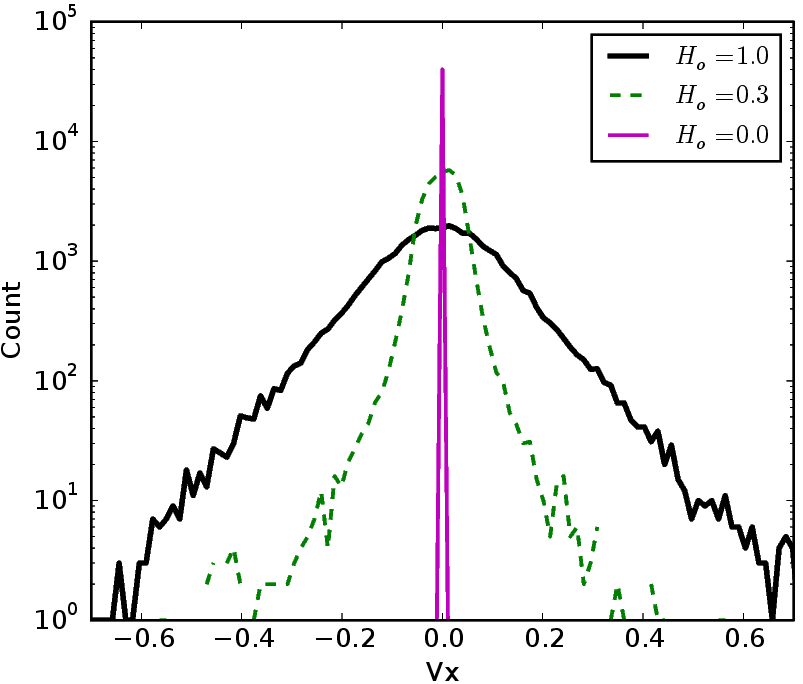
\includegraphics[width=\textwidth]{Figures/2_Vx_histogram_2}
        \caption{Distribution for different \tHub}
        \label{Fig:2_Vx_histogram_2}
    \end{subfigure}
\caption{(a) Distribution of the one-dimensional velocity field for the whole cluster as the thick solid black line, in the simulation labelled as R40h20 at the apex time (H$ = 0$). The red dashed distribution matches clump members and thin solid blue the field particles. (b) The distribution for three different values of \tHub: when $\Hub_0 = 0$, the distribution is a Dirac-$\delta$ around $v = 0$. The central distribution broadens as \tHub increases to 0.3 and 1. Observe the exponential profiles at large $|v|$. Velocities are in H.u} 
\label{Fig:2_Vx_histogram}
\end{figure}




 There is no hydrodynamics in the approach that we have taken, nevertheless expansion under gravity alone is equivalent to the adiabatic expansion of gas~: for that case, the first law of thermodynamics equates the drop in internal energy ${\rm d}U$ to minus the external work,  $-p {\rm d}V$. At constant mass, the change in gravitational energy ${\rm d}W$ is $ - {\rm d}E_k$, where $E_k$ is the kinetic energy. With $W < 0 $ but increasing over time, this implies that $E_k$ drops in amplitude. In the case when the motion is strictly radial, $E_k = 0$ when $H = 0$ and all stars come to rest. We ask to what extent the growth of substructures and non-radial motion  off-set the `adiabatic cooling' brought on by expansion. 

Fig.~\ref{Fig:2_Vx_histogram_1} graphs the x-axis one-dimensional velocity distribution for the R40h100 model. The left-hand panel displays the overall distribution as well as the two sub-populations of clumps members and out-of-clump \textit{field} stars. We identified some 20944 stars in clumps (or $\approx $ 52\%) at the end of expansion. The expectation that all stars have zero- or low-velocities is validated by the peak in the distribution around $v_x = 0$.

As sub-structures form and  interact mutually, generating tangential as well as radial motion, the peak broadens but remains symmetric about the origin.  The large velocities are brought by stars in clumps, which demonstrates that interactions within the substructures boost the internal velocity dispersion of the cluster as a whole. Field stars dominate the low-amplitude regime. Their velocity distribution is well-fitted with a  Gaussian (shown as a dotted blue line), down to one-tenth the height of the central peak, or about 1\% of all field stars. 

To illustrate further the idea that large velocities are confined to clumps formed by fragmentation modes, we compare on Fig.~\ref{Fig:2_Vx_histogram_2} a set of models 
with different initial  values of  $\Hub_o$: 0, 0.3, and 1. 
Clearly when $\Hub_o=0$, the velocities are identically zero and there is no fragmentation whatsoever (apart from root-N noise). The distribution is then a sharp peak centered on zero. For positive but low values of $\Hub_o$, the fragmentation modes do not develop much before the apex and the (non-radial) velocities remain small. The central peak  has a much narrower dispersion, and the high-velocity wings are clipped. In this case, too, analysis of the  weakly fragmented system shows that virtually all high-velocity stars are found in clumps. The velocity distribution for the case  $\Hub_o = 1$ is added for comparison. The fact that the full range in velocities is reduced by a factor $\sim 3$ for the 
less fragmented model is also an indication of the shallower potential well of the clumps

The full population velocity distribution (solid black line) at first sight is very similar to those of \citet[Fig.~5]{Klessen2000}. In that figure, the authors show the velocity distribution of gas particles in a fragmenting system. \citeauthor{Klessen2000} attribute the high-velocity tails to gas particles falling towards stellar clumps at supersonic speed. Supersonic motions imply that gas particles trace ballistic trajectories, and hence behave like point mass particles. 

A small fraction of field stars in our calculations also have large velocities. We suspected that these stars might have acquired their large velocity through in-fall toward a nearby stellar clump. We did not, however,  find compelling evidence that would allow us to identify the origin of high velocities in field stars. Inspection of a sequence of snapshots failed to show that the velocity vectors were pointing at nearby stellar clumps: it is therefore not possible to make the same assertion as \citeauthor{Klessen2000} and state that stellar clumps accrete some field stars.

It is possible, on the other hand,  that high velocities originate from past star-star interactions. However, we did not find clear trends in the few orbits that we studied which would confirm such an event. The question of mass accretion by stellar clumps might be best settled if we added gas to our simulations to boost the mass resolution, and analysed model data using mock CCD frames, as did \citeauthor{Klessen2000}. This was not attempted here.

We close this section with a remark about the velocity distributions seen on Fig.~\ref{Fig:2_Vx_histogram} and the internal state of the stellar clumps. Because small clumps would have time to evolve dynamically through star-star collisions and reach a state of near-equilibrium (see \S\ref{Sec:Timescales}) we would expect clumps to develop a velocity field similar to Mitchie-King models of  relaxed self-gravitating star clusters \citep{BT}.  The one-dimensional velocity distribution of Mitchie-King models plotted in a logarithmic scale approaches a flat-top when $|v_{1d}|$ is small,  and cuts-off rapidly at large values~: the distributions are  concave at all velocities. This holds true for all models independently of their King parameter\footnote{Notice how this holds only because of the choice of a logarithmic vertical axis.} $W_0$. 

The shape of the distributions displayed on Fig.~\ref{Fig:2_Vx_histogram}, on the other hand, is convex as we shift, from small, to large $|v_{1d}|$. We deduce from this straightforward observation that the clumps that formed through fragmentation and subsequent mergers cannot be treated as fully in isolation and in dynamical equilibrium \`a la Mitchie-King.  Fragmentation in hydrodynamical calculations often proceeds from filaments and knots  (e.g., \citealt{Klessen2001,MacLow2004,Maschberger2010,Bate2014}). The clumps that form in a fragmenting  Hubble  flow are also surrounded by filaments and other structures which perturb them.




\subsection{The stellar mass function in clumps} 



We show on Fig.~\ref{Fig:2_ClumpMembers} the mass function of stars both in clumps, field and in the whole cluster. For brevity, we only show a model with a mass function truncated at $20 M_\odot$, Rmh20,  however our conclusions are not sensitive to the truncation value. The mass function of $\approx 6400$ stars that were found in clumps (some 43\%) is displayed as the red solid curve and all other stars, field stars, as the blue solid curve. The theoretical Salpeter distribution function for the same number of stars is shown in black dots, with grey shades giving the  $1 \sigma$ dispersion from multiple samplings. Finally, the green dashed curve  shows the mass distribution of all 15 000 stars in the model. The lower panel is the same data normalised to the Salpeter data. 

The uptake  in massive stars for the whole population (green dashed line) of both clumps members and field stars is a statistical artefact and lie within the standard deviation of a Salpeter distribution with comparable sampling number. 

The clump member population clearly deviates from a Salpeter distribution in two ways~: first we note a deficit of low mass stars with respect to the theoretical Salpeter; secondly, although a Salpeter mass function is more or less consistent with the population up to $M\approx 2M_\odot$(black dotted line) the distribution shows a clear excess of massive stars. We find that practically all the stars more massive than 10$M_\odot$ ended up in a clump (this is the point where the solid red curve joins the dash green one). 

A linear regression fit of the clump members mass function gives a power-law index of $-2.15 \pm 0.02$, shallower than the Salpeter index of -2.35. Applying the same analysis to field stars,  we find a steeper mass function of index $-2.46 \pm 0.02$. The difference of $\approx 0.3 $ between the two populations is very similar to what is found in the Milky Way disc (see e.g. \citealt{Czekaj2014,Rybizki2015,Bastian2010} )

\begin{figure}
\begin{center}
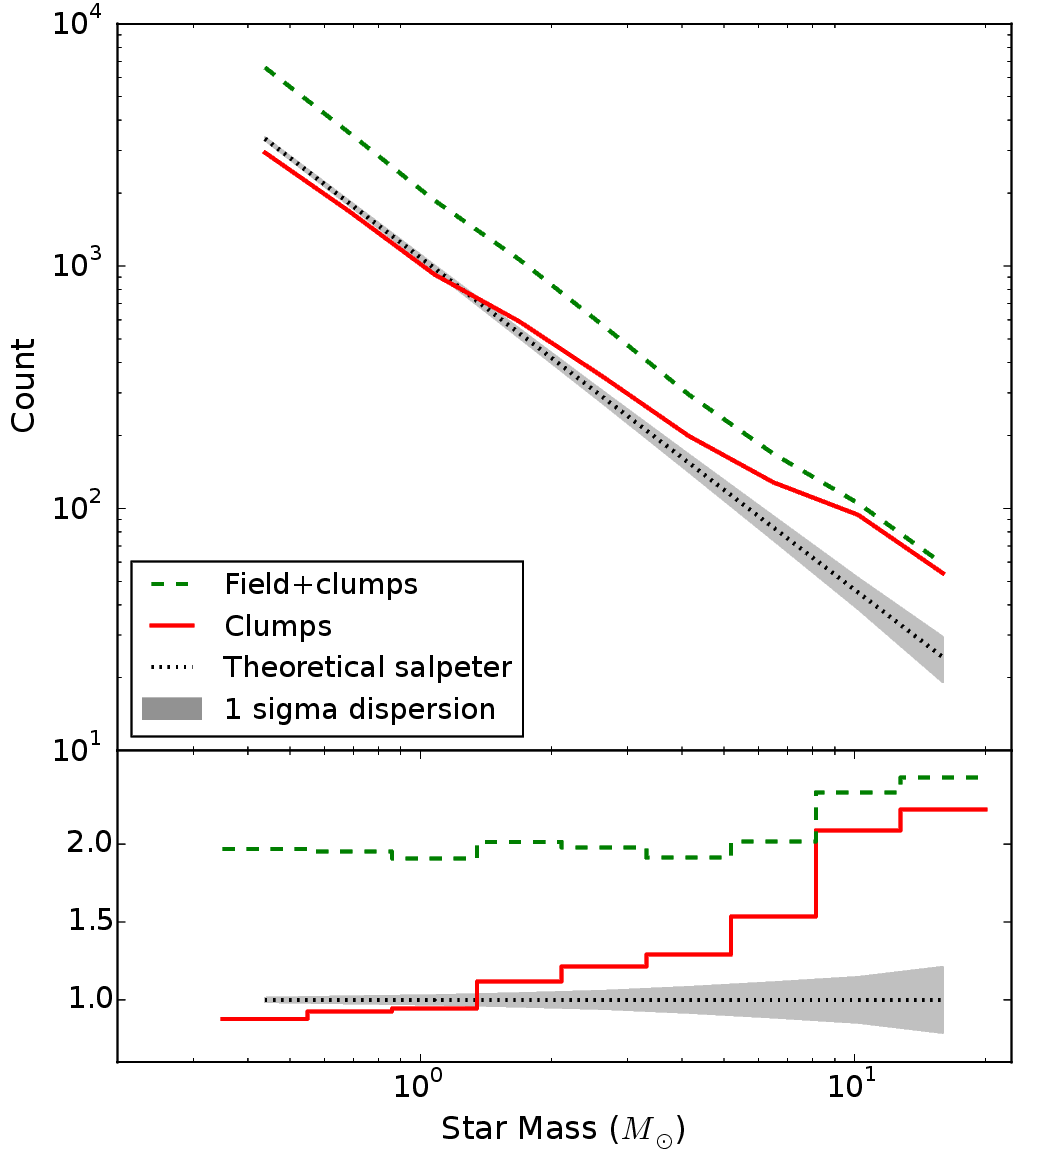
\includegraphics[width=0.8\textwidth]{Figures/2_ClumpMembers}
\caption{Top panel~: Mass function of all stars belonging to a detected clump (solid red). The expectation drawn from a Salpeter distribution function for the same total number of stars in dotted black~; the grey shade are $1\sigma$ uncertainties. The green dashed line is the  distribution for the full cluster. Bottom panel~:  same data normalised to the Salpeter expectation.}
\label{Fig:2_ClumpMembers}
\end{center}
\end{figure}

\cite{Bonnell2004} and \cite{Maschberger2010} showed from inspection of  hydrodynamical simulations that massive stars play a key role in the assembling process of clumps, attracting already formed protostars to them. We find  a similar general trend in Hubble-fragmented gas-free simulations: clumps develop around massive stars so that their stellar mass function is top-heavy. 

This excess can also be seen in the top panel of Fig.~\ref{Fig:2_MaxMass} in which for each of 440 clumps, we show as white dots the mass of their heaviest star as a function of the host clump's mass. These data were obtained from the R40h100 run. For comparison, we sampled a Salpeter mass function, drawing the same number of stars as found in each clump. We then identify the most massive star in the Salpeter sample~; the procedure was repeated 15000 times {\it for each clump} to obtain suitable statistics. The grey shades (color levels in the electronic version)  shows the resulting distribution.



 \begin{figure}
\center
    \centering
    \begin{subfigure}[b]{\textwidth}
    	\centering
    	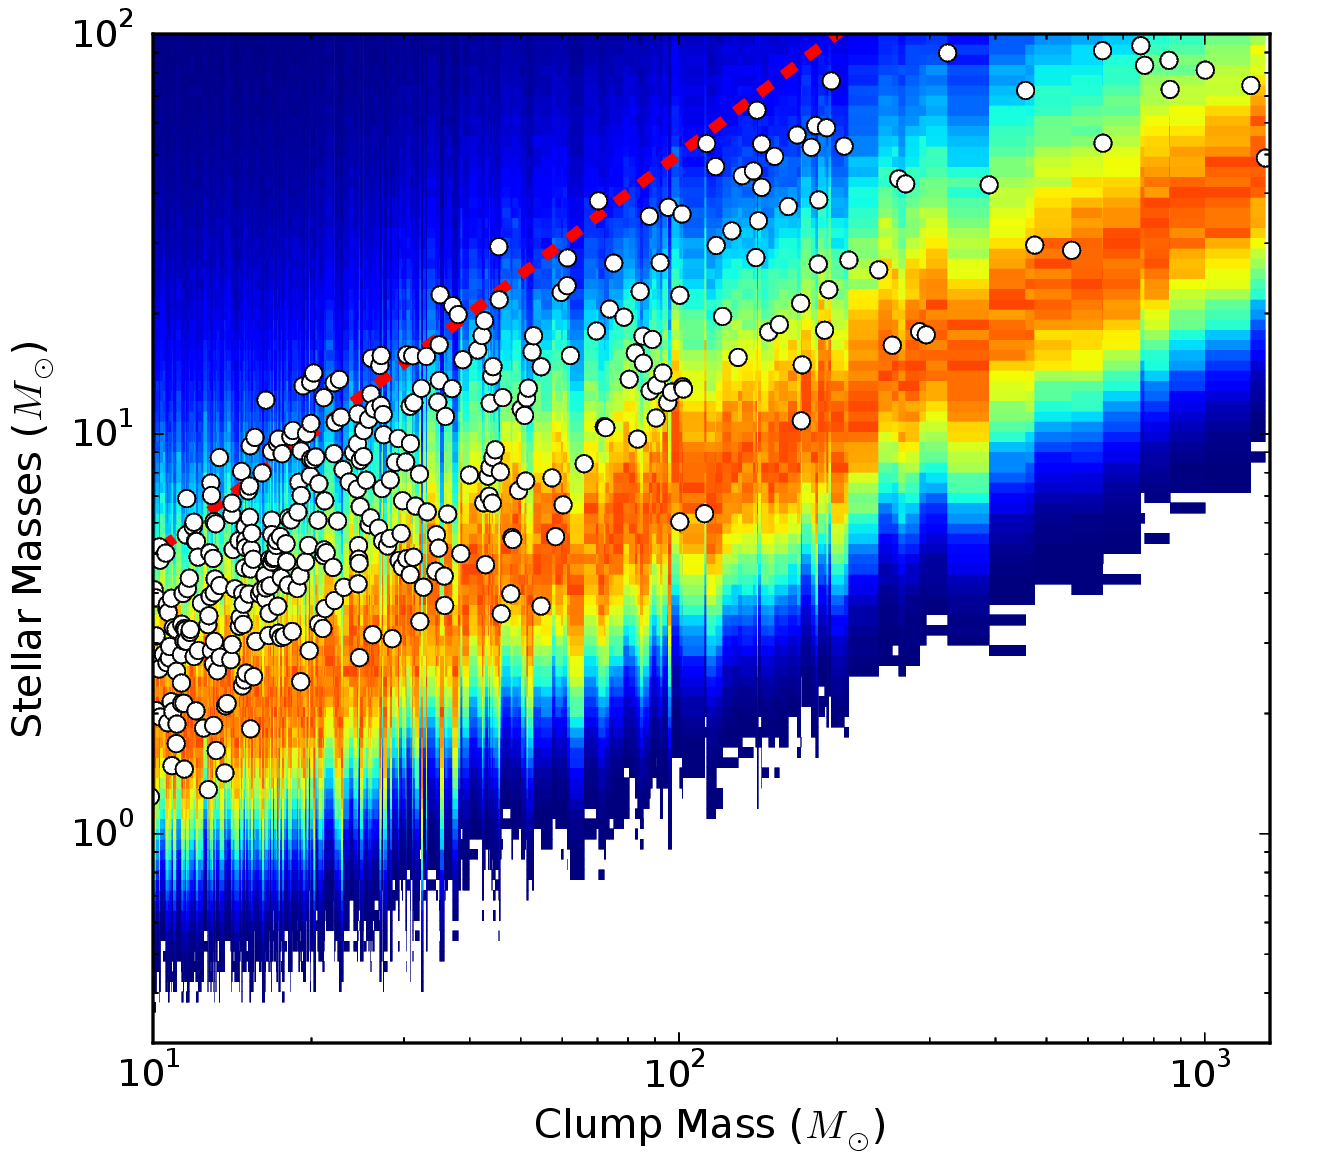
\includegraphics[width=0.7\textwidth]{Figures/2_MaxMass}
        \caption{Distribution clumps/field}
        \label{Fig:2_MaxMass}
    \end{subfigure}
    \begin{subfigure}[b]{\textwidth}
    	\centering
    	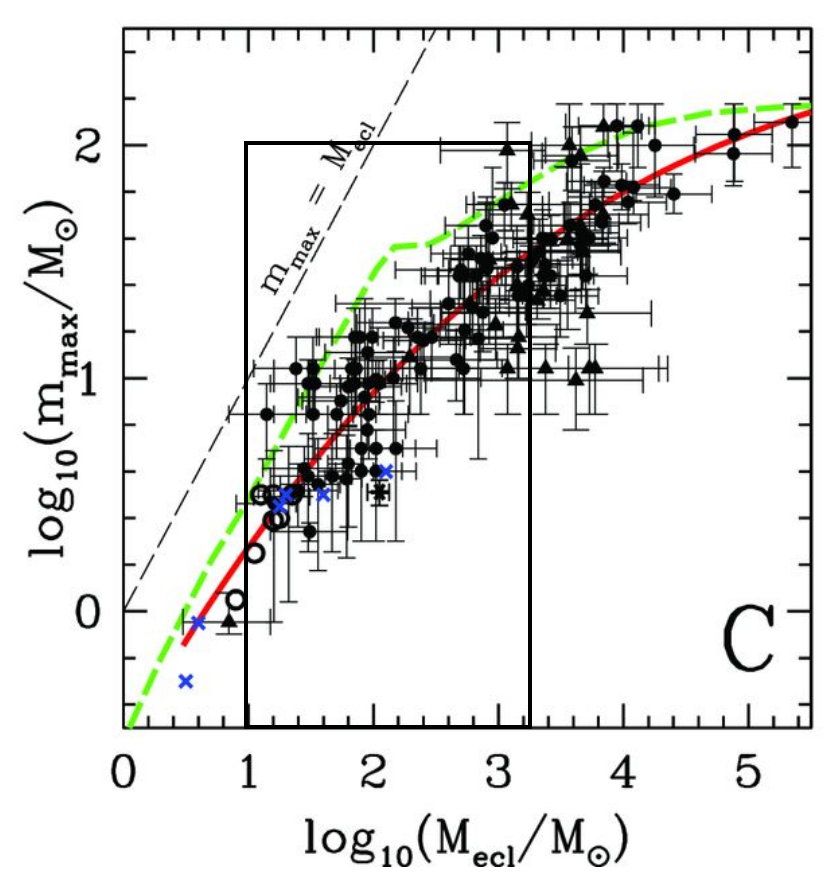
\includegraphics[width=0.6\textwidth]{Figures/2_weidner}
        \caption{Distribution for different \tHub}
        \label{Fig:2_weidner}
    \end{subfigure}
\caption{(a) Mass of the heavier star in each clump, shown as white dots, as a function of clump mass. The color map shows the likelihood for the maximum mass if all clump members were  sampled from a Salpeter IMF~; the orange crest gives the maximum likelihood. The red dashed line shows the  relation $m_{clump} = 2 m_{max}$ (see. section \ref{Sub:2_ClumpMF_MF}). The data was taken from the R40h100 run. (b) is a similar distribution from \protect\cite{Weidner2013}, built with data about young embedded star clusters from \cite{Weidner2010}. The black frame notes the range of masses displayed in (a). } 
\label{Fig:2_McMmax}
\end{figure}


 In a nutshell, Fig.~\ref{Fig:2_MaxMass} shows for each clump the likelihood that their most massive stars may be drawn from a Salpeter function, one could call the red maximum likelihood zone the "Salpeter valley". Only clumps with a mass $> 10 M_\odot$ are included to account for a possible bias when clump membership reaches below $N_d =12 $ stars. It can be seen on the figure that the scatter of white dots tends to lie systematically above the Salpeter valley. If we add the  relation $m_{clump} = 2\max\{m_\star\}$ (cf. section \ref{Sub:2_ClumpMF_MF}), we find some overlap with the data (see the red dashed line on Fig.~\ref{Fig:2_MaxMass}). This clearly illustrates the tendency for massive stars to act as seeds when the clump form, while the scatter is driven by the merger and accretion history of individual clumps. 
 
 The correlation displayed on Fig.~\ref{Fig:2_MaxMass} is in good agreement with observational data for young embedded clusters of the same mass range published by \citealt{Weidner2013}. We reproduced their figure on Fig.~\ref{Fig:2_weidner} with a black frame representing the range shown on Fig.~\ref{Fig:2_MaxMass}. 
 
 Note how the {\it scatter} in the correlation brought on by the dynamical processes at play during the adiabatic fragmentation phase also compares well with the data. Thus the stellar clumps modelled here recover an important characteristic of observed embedded young clusters.
 





\subsection{Mass segregation}
\label{Sec:2_ClumpSegregation}

In this section, we ask whether the clump assembling process at play in our simulations accounts for the mass segregation measured  in  star-forming cores in hydrodynamical simulations. The measure of mass segregation of \cite{Olczak2011} based on the MST, while efficient, will give noisy results for very small-N clumps. Instead, we follow \cite{Maschberger2010} and rank clump members according to their distance to the geometric centre of a clump, which is calculated by number-averaging (so this centre is not the clump barycentre). We then sort the bodies by mass and tabulate the radial rank of the three most massive ones. This process is illustrated on Fig~\ref{Fig:2_radial_ranking}.


\begin{figure}
\begin{center}
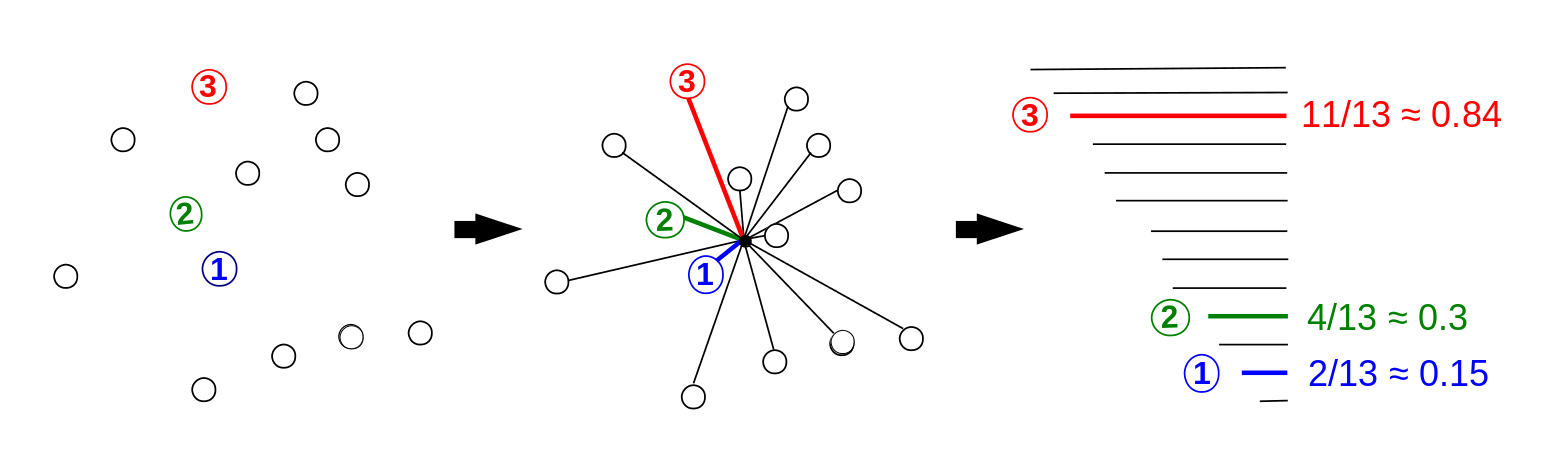
\includegraphics[width=\textwidth]{Figures/2_radial_ranking_schema}
\caption{Illustration of the radial ranking method. Stars marked 1,2 and 3 are the first, second and third most massive stars in the clump. Distances to the geometrical center are computed then sorted. The position in the sorted list is converted to a number, the radial rank.}
\label{Fig:2_radial_ranking}
\end{center}
\end{figure}

The great advantage of this approach is that it is independent of geometry and absolute size once the ranking is normalised to the clump membership $N_c$.  One issue arises with the binning of the rank, since small values of $N_c$ give large intervals by construction, and conversely for populous clumps~: we found a good compromise by setting the width of each bin to 1/20 since the mean clump mass $\sim 20 M_\odot$ implies $N_c \sim 20$ on average. The procedure is repeated over all clumps identified in the run (typically on the order of $\sim 200$). The diagnostic for an un-biased sampling is a profile with radius that remains the same regardless of the mass selected~; if, furthermore, the stars are (on the mean) un-segregated in radius, then the profiles will be flat. 


Fig.~\ref{Fig:2_ClumpSeg} graphs the  distribution of rank of the three most massive stars in all the clumps from R40h100 fragmented state. The salient features are that 1) none of the distributions are flat, all three peaking significantly  at small ranks~; and 2) there is a clear trend for the most massive star also to be the most  segregated. Precisely this result had to be expected from the internal dynamics of small clumps (cf. section~\ref{Sec:Timescales}).  Our Fig.~\ref{Fig:2_ClumpSeg} should be compared with Fig.~13 of \cite{Maschberger2010}: the authors also found radial rank distribution to peak at small values for massive stars, showing a level of mass-segregation in their clumps.

It is striking that the measure of mass segregation attained here for a gas-free configuration is a good match to a full hydrodynamical setup. By implication the segregation proceeds more vigorously once the proto-stellar cores have condensed and behave essentially like point sources. The initial configuration that we have adopted relies only on density fluctuations to seed clumps, however once again we find evidence that massive stars begin and remain the centre of gravitational focus for clump formation. That is not so when clumps are setup using a fractal approach \citep{Goodwin2004,Allison2009}. There is then no segregation initially, and it all develops at or shortly prior to the global system evolution towards equilibrium (the collapsing violent relaxation phase). 


\begin{figure}
\begin{center}
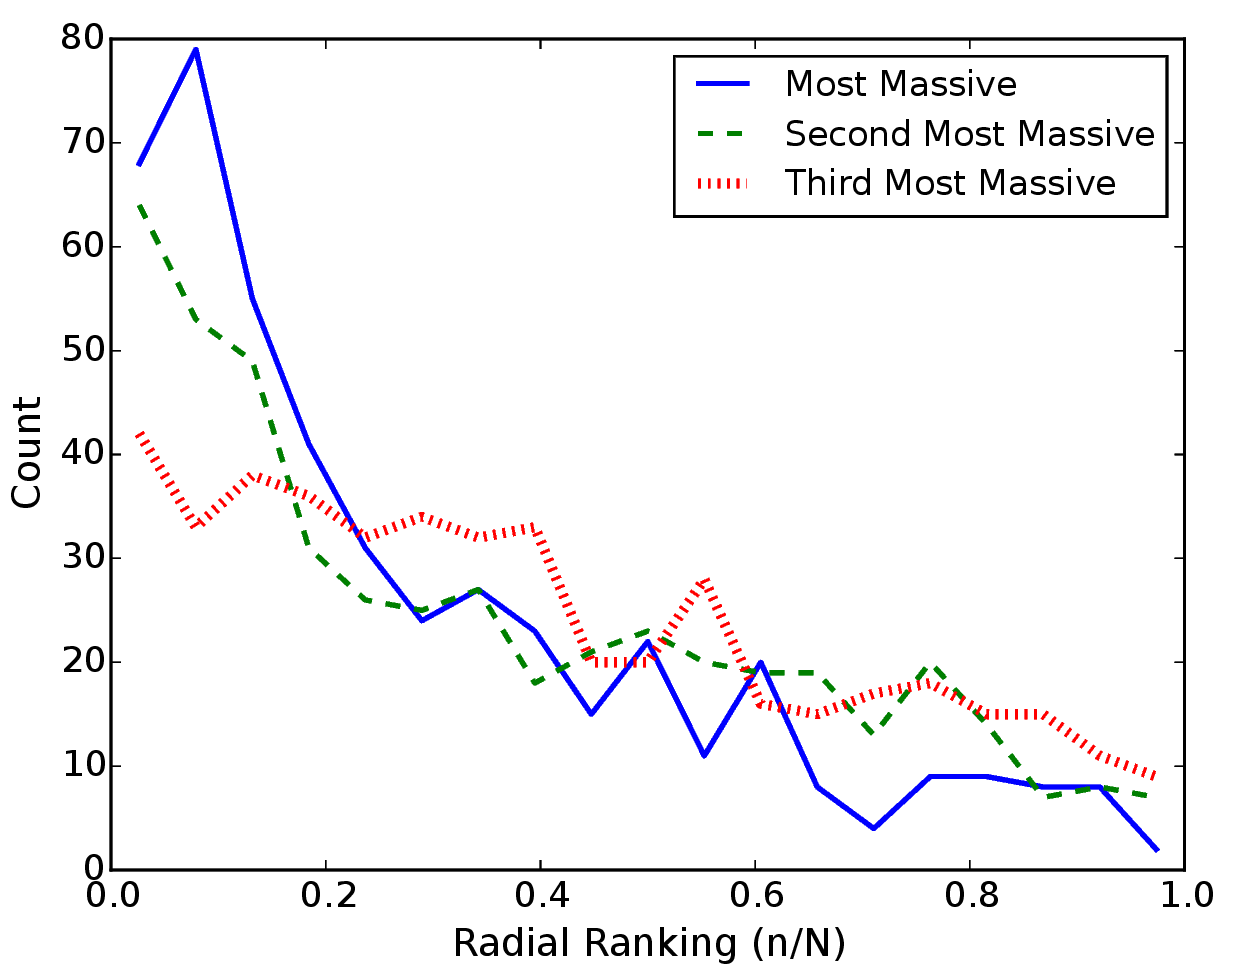
\includegraphics[width=0.6\textwidth]{Figures/2_ClumpSeg}
\caption{Histograms of radial ranking of first, second and third most massive star in each clump for a model with N = 40 000 stars (R40h100).}
\label{Fig:2_ClumpSeg}
\end{center}
\end{figure}







\section{Concluding remarks}


We have developed a new approach based on adiabatic fragmentation to set up self-consistent configurations for stellar dynamics that link up the velocity field of stars to their irregular space configuration of arbitrary geometry, such as knots or filaments. The method offers great advantages: it is easy to implement; it can treat an arbitrary number of stars without any resolution issue; furthermore, the level of fragmentation can be tuned through the Hubble parameter. The light computational load allows for statistical ensemble averaging over large samples, as was done throughout this chapter. For instance, the computation time on a single card for 80,000 stars is about 12 hours. The methods has its limitations: the most significant one is the failure to include hydrodynamical effects. In the introduction, we mentioned other approaches partly based on hydrodynamics: such hybrid methods have been successful but remain limited in scope, for instance \cite{Moeckel2012}, or demanding in computational resources (and so constrain the number of realizations), as in \cite{Fujii2016}. 

\subsection*{The importance of massive stars}


During the fragmentation process in our models, heavy stars act as seeds for the growth of stellar clumps, and so the stellar clumps mass spectrum is shaped by the mass function of the available {\it stars}. Although the fragmentation through gravitation only does not include the detailed physics of star formation, we noted that hydrodynamical calculations including gas pressure and turbulence suggest that the gravitational potential of massive stars attract more gas and stars and, as such, act act as seeds for the formation of clumps \citep{Bonnell2004}. We therefore recover a key prediction of hydrodynamical simulations. It is then interesting to ask whether observations show a correlation between the host clump mass and its population of massive stars.

 Based on analysis of our fragmented Hubble models, we recover on Fig~\ref{Fig:2_McMmax} a correlation between the maximum mass of a star found in a clump of a given mass, $M_c$. This $\max\{m_\star\} - M_c $ relation is eerily similar to the compilation for young clusters by \citet{Weidner2013}, from which we extracted the figure \ref{Fig:2_weidner}. Furthermore, we also found that the stellar mass function in clumps has a much flatter (top-heavy) profile than in the field, {\it i.e.} stars that do not belong to any clump: power-law fits for the two stellar populations show that the Salpeter index for clumps stars is lower by about $\approx 0.3$ compared to the same index for field stars. A similar difference is deduced for Milky Way data ( \citealt{Czekaj2014,Rybizki2015}; see also Fig 2 from \citealt{Bastian2010}):  we argue that these characteristics will help tighten our understanding of the long-term evolution of such stellar associations, given that their properties are, on the out-set, close to actual data for young clusters. It should be emphasised that the global index of external galaxies may differ significantly from the canonical value $\alpha = 2.35$ ({\it e.g.}, the GAMA survey, \citealt{Gunawardhana2011}; see also \citealt{Hoversten2008}). We have not explored here to what extent this difference in indices  between field and clump populations will change for other values of the global index $\alpha$.

We have also noted that the clumps are {\it mass segregated} at birth, i.e. at the end of the fragmentation process. When we apply the same ranking statistics as for hydrodynamical calculations of star formation, we obtain the same level of segregation for the three most massive stars in a clump (cf. Fig. \ref{Fig:2_ClumpSeg}). %Heavy or light stars caught in dense clumps have high velocities, while  only a small fraction of field stars have such large velocities: we found that the velocity distribution function of field stars is well fitted with a Gaussian, except for the $\sim 1\%$ with the most extreme velocities. We drew a comparison with the SPH calculations by \cite{Klessen2000}, who attributed the high-velocity tail of gas particles to their in-falling onto stellar clumps. However, we could not identify unequivocally the origin of the large velocities for the field stars (past star-star interactions, attraction by a clump, .. ). That point may well be worth exploring in a future study, as it relates to the likelihood of accretion of field stars by a dense stellar clumps. Recent SPH calculations by M. Bate and collaborators hint at continued exchanges between stellar cores and their environment.

\subsection*{The slope of the clump mass function}

\cite{Klessen2000,Klessen2001} fit the gas clump mass function of their simulations with a power-law of index -3/2. On the other hand, the \textit{cluster} mass function in the Milky Way can be described as a power law $\frac{dN}{dM} \propto M^{-\beta}$ where $\beta$ takes value ranging from -2 to -2.4 \citep{Haas2010}. We have indicated that a power-law relation with a slope $ \beta \simeq -4$ is a rough fit for the case where all the stars are identical (Fig.~\ref{Fig:2_ClumpMF_MF}). This is not so  when a stellar mass spectrum is included~: if a Salpeter distribution function is truncated at $20 M_\odot$ a power-law with slope $ \beta \simeq -1.7$ still fits approximately the distribution of clumps of  mass $ > 20\, M_\odot$~; and when the Salpeter distribution function is truncated at $100 M_\odot$, a power-law similarly fits the tail-end of the distribution but now with a slope of $\simeq -1$ (see Fig.~\ref{Fig:2_ClumpMF_MF_2}). It is intriguing that the slope of the distribution should fall within the bracket of values for the observational data for clusters ($-2.4^+$) and hydrodynamical fragmentation models (-3/2). If the clumps formed from hydrodynamical fragmentation should become individual star clusters, and recover the $\beta \simeq -2 $ or lower slope of observational data, then the distribution function must become steeper and also cover a broader range of masses. The same conclusion applies to the Hubble clump distribution function.

This implies either that clumps will merge so that a few very massive clusters will emerge, or that fewer massive clumps form in the first place. Comparison with existing cluster population needs us to assume these clumps do not fall back and merge through collapse. This is possible with an adequate galactic tidal field ripping apart this fragmented configuration and isolating the clumps before the collapse. Many of the small stellar overdensities detected as clumps would not survive more than a few million years before dispersing through dynamical interaction, however the larger clumps could survive and appear as isolated cluster or part of an association. These massive clumps   are the key to comparison to the galactic cluster mass function. We have shown how the stellar IMF provides seeds for the growth of massive clumps and have illustrated this with a Salpeter power-law IMF. A more realistic  IMF has a steeper power index at larger stellar masses \citep{Kroupa2002,Chabrier2005}. The fragmentation of stellar systems with fewer massive stars would deplete the clump mass function at larger masses more in line with observed statistics for clusters. 
This variability in the clump mass function highlights the major influence of the stellar IMF on the fragmentation process. A full exploration of fragmentation requires hydrodynamical simulations, which we have not performed here. These simulations remain limited to much smaller systems \citep{Bate2014,Lomax2014}.

\paragraph*{}
In the next chapter we assume an absence of tidal field and follow through with the final stage of evolution towards equilibrium. We compare the final configuration with those of \cite{Allison2009} and the recent study by \cite{Caputo2014}. 
    

\chapter{Collapse and dynamical evolution}


In this chapter, we let the \HubLem models evolve and undergo violent relaxation. We compare their dynamical evolution with that of cold uniform models. We investigate the evolution of the structure and global mass segregation.

\minitoc

\section{The simulations}
\label{Sec:3_simulations}

\subsection{Description of the models}

The \HubLem fragmented system is subvirial by construction. The configuration we took as a reference is the apex of the expansion: the kinetic energy initially injected in the expansion has been converted into potential energy through expansion or converted to transversal motion by two-body interaction. If the model is left to evolve further, it collapses, violently relaxing to reach a quasi-equilibrium state, resembling a Plummer or King model.

In the present chapter, simulations will use the fully fragmented state of Hubble models as initial conditions for the subsequent dynamical evolution. Observational clues point to  collapsing and violently relaxing clusters. For example, \cite{Cottaar2015} find IC 348, a young (2-6 Myr) cluster, to be both survirial and with a convergent velocity field, consistent with infalling motion. Our models undergo dry collapse with no gas, while real objects such as IC 348 still contain residual gas. The scenario of our simulations is an idealized situation: clearly if there was residual gas between the clumps and it was evacuated through stellar feedback, both the clump merger rate and the depth of the potential achieved during relaxation would be affected. As a limiting case, rapid gas removal may lead to total dissolution (see for instance \citealt{Moeckel2012} and \citealt{Fujii2016}). In the current situation, all clumps will merge. 


The numerical integration were done once more with the NBODY6 integrator with the same computational units. For comparison purposes, we also performed simulations of cold uniform spheres, a configuration which has been extensively used  in the past (e.g.,\citealt{Theis1999,Boily2002,Barnes2009,Caputo2014,Benhaiem2015}) and one that minimises the level of fragmentation and mass segregation in the on-set of collapse. The models are referenced as Rh100, Rh20,Ru100 and Ru20 in Table~\ref{Tab:2_models}. The aspects of Rh20 and Ru20 during collapse are shown on Fig~\ref{Fig:3_collapse}. Note the deeper collapse of the uniform system.

 We focus here on models with a mass function from 0.35$\Mo$ to 20$\Mo$ and 15000 stars, a compromise value for rich open clusters that should allow us to identify clearly collisional effects and trends with time, and ease comparison with the recent study by \cite{Caputo2014} where most calculations are performed with that sampling. We let both Hubble-fragmented and uniform sphere evolve up to 40 H.u. 





\begin{figure}
\begin{center}
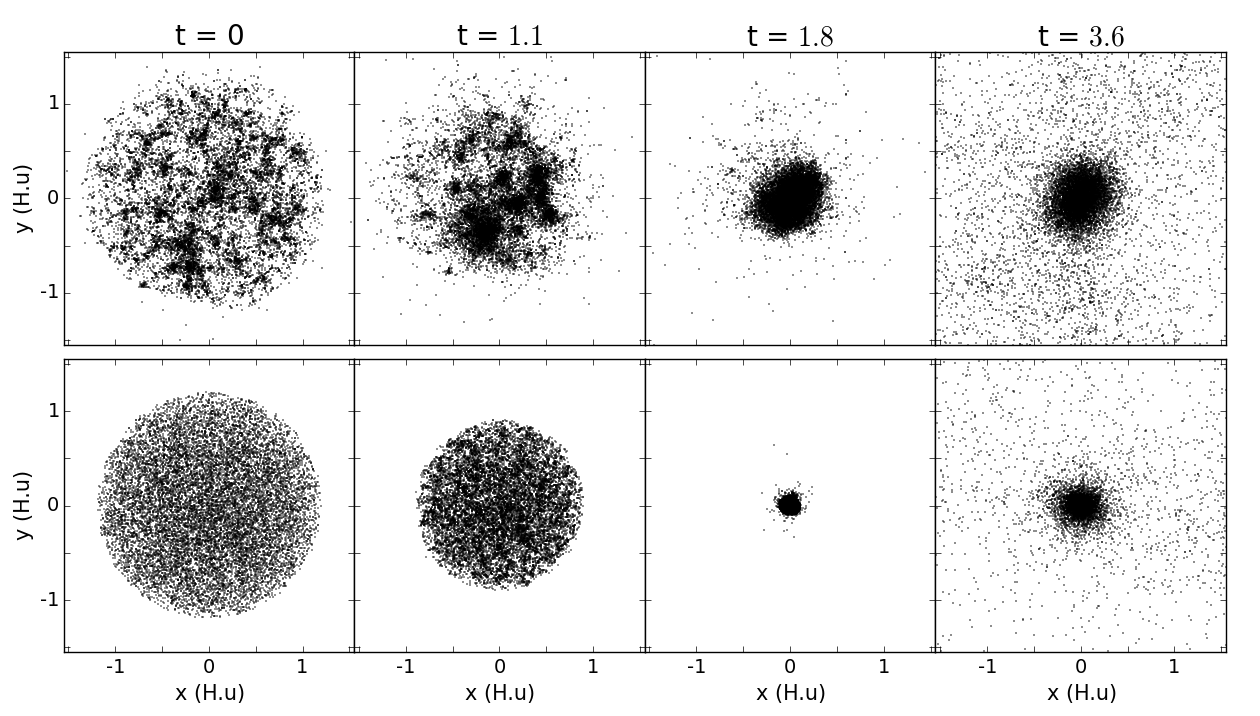
\includegraphics[width=\textwidth]{Figures/3_collapse}
\caption[Stages of collapse for HL fragmented and uniform models]{Aspects of both Hubble (top panels) and uniform (bottom panels) systems throughout the collapse. The epochs shown are, from left to right: initial conditions; half-collapse; point of deepest collapse; direct aftermath of collapse. The times are in H\'enon units.}
\label{Fig:3_collapse}
\end{center}
\end{figure}


\subsection{Scaling to physical units}
\label{Sec:3_Scaling}
Before discussing the results, it is useful to translate the units of computation to physical scales. This is important if we want to discuss the state of the systems using one and the same physical time, such that the hypothesis of no stellar evolution holds.
To do so, we compute the free-fall time of an uniform sphere (a good approximation for fragmented model as well) both in physical units and H\'enon units, which provide a conversion factor. We first have to choose an initial physical length scale for the system by setting $R_h = 1$ pc. With a total system mass of $M = 15\cdot 10^3\, \Mo$, this gives the uniform half-mass volume density 
\begin{equation}
\rho_h = \frac{M/2}{\frac{4}{3}\pi r_h^3}  \simeq 1.8 \cdot10^3 \Mo / pc^3,
\end{equation}
within values typically inferred from observations of clusters.

 The free-fall time of an uniform sphere, obtained from conservation of energy and integration, is expressed as
\begin{equation}
t_{ff} = \sqrt{\frac{3\pi}{32 G \rho_{h	}}}.
\end{equation}
Computing $\rho_{h,\textrm{H\'enon}} \simeq 0.13$, we now compute both values of the free-fall time
\begin{align}
t_{ff} &\simeq 1.5~ t_\Hen\\
	   &\simeq 0.2~ \Myr
\end{align}
which gives: 
\begin{equation}
1 ~ t_\Hen \equiv 0.13~ \Myr = 1.3 \cdot 10^5 \yr .
\end{equation}


Thus by running up to 40 H.u we ensure that the systems evolve for $ \sim  6~\Myr $, about the lifetime of a 50$\Mo$ star. \footnote{For our models with more massive stars, up to 100$\Mo$, these represent only $\sim$ 5\% of the total mass and their removal would not significantly alter the dynamics of the system.}

We now want to evaluate the crossing and relaxation time-scales in such a system, as they were defined in the introduction (\ref{Sub:0_time-scales}), and how they relate to the total duration of the simulation. We could attempt to derive a crossing time for the initial, subvirial state but it would not be representative of the evolution of the system. Instead, the more useful crossing time has to be computed from the equilibrium state achieved. Using the virial theorem and conservation of energy, we derive dynamical time-scales for the equilibrium system. The crossing times is defined as
\begin{equation}
\label{Eq:3_tcr}
t_{cr,eq} = \frac{2 R_{h,eq}}{\sigma_{1d,eq}}.
\end{equation}

From here on, we write the subscript 0 for initial values and no subscript for equilibrium values. To obtain both $R_{h}$ and $\sigma_{1d}$ we start from the total energy of the system. At t=0, velocities are null, all energy is potential energy. It can be computed by integrating from the center to $R_0$. We obtain
\begin{equation}
E_0 = - \frac{3}{5} \frac{G M^2}{R_0}.
\end{equation}
From virial theorem and conservation of energy, we get the following equations at equilibrium
\begin{equation}
\label{Eq:3_energies}
\begin{cases}
2 E_k + E_p &=0\\
E_k + E_p &= E_0
\end{cases} 
\quad
\implies
\quad
\begin{cases}
E_k &= -E_0 = \frac{3}{5} \frac{G M^2}{R_0}\\
E_p &= 2 E_0 = - \frac{6}{5} \frac{G M^2}{R_0}.
\end{cases}
\end{equation}
which can be combined with
\begin{equation}
E_k = \frac{1}{2} M \sigma_{3d}^2 = \frac{3}{2} M \sigma_{1d}^2
\end{equation}
to get
\begin{equation}
\sigma_{1d} = \sqrt{\frac{2 G M}{5 R_0}}.
\end{equation}

As for the half-mass radius at equilibrium, its value is dependant on how concentrated the system is and is not easy to derive. However, numerically obtained King models show that in relaxed systems, there is a consistent relation between $R_h$ and the virial radius $R_v$, defined as 
\begin{equation}
\label{Eq:3_virialradius}
E_p = - \frac{G M^2}{2 R_v},
\end{equation}
that gives 
\begin{equation}
\label{Eq:3_radii}
R_{h,eq} \approx 1.3 \times R_{v,eq}.
\end{equation}

 Combining Eq.~(\ref{Eq:3_energies}),~(\ref{Eq:3_virialradius}) and~(\ref{Eq:3_radii})  it comes
\begin{equation}
R_{h,eq} \approx 0.54 R_0.
\end{equation}


Knowing that $R_0 = 2^{1/3} R_{h,0}$, we now write a good approximation of the crossing time in the relaxed, equilibrium system
\begin{align}
t_{cr}  &\simeq 1.7\frac{R_0^{3/2}}{\sqrt{GM}}\\
        &\simeq 2.4~ t_\Hen\\
	    &\simeq 0.3~ \Myr.
\end{align}

 With $N = 15 000$  we find from (\ref{Eq:0_trel}) a two-body relaxation time-scale

\begin{align}
t_{rel}  &\simeq 324~ t_\Hen\\
	     &\simeq 95~ \Myr
\end{align}

and from (\ref{Eq:0_ms2}), considering a mass range of $m_{max}/\langle m\rangle = 20$, we find a mass-segregation time-scale

\begin{align}
t_{ms}  &\simeq 25~ t_\Hen\\
	    &\simeq 7.5~ \Myr
\end{align}

Our simulations last for far less than a relaxation time, but we expect to see some dynamical mass segregation set in in our models.


\subsection{Removal of the ejected stars}

In the previous section, we considered there was no mass loss during the collapse and relaxation that lead to the equilibrium system. However, a look at the simulations shows this assumption does not hold. Some stars are ejected from the system after the collapse, when the system bounces. These stars are not part of the equilibrium system as they have no influence on the central dynamics.

To investigate the evolution of the central bound system only, we need to isolate and substract the ejected stars. The obvious way to do this would be to compute the stars mechanical energies and to remove all stars with positive energy. Though this works for a majority of the ejected stars, a subset of them has a marginally negative energy. These register as bound when they are essentially out of the system (far beyond the original system radius). 

To efficiently collect a maximum number of ejected stars, we spotted the time when the potential energy is maximum, when the collapse occurs. We  then identified all stars whose distance to the center increased monotonically from there onwards. The full selection criteria is therefore~:

\begin{equation}
v_r(t) > 0,~\forall t > t_{ff}\quad \textrm{or} \quad  E_\star > 0 , ~\forall t > t_{ff}
\end{equation}
 
This allows a more complete selection of the ejecta.  On Fig.~\ref{Fig:3_DistOrigin} we graph  $|\bold{r}|$  as a function of time for a subset of escapers (shown as red curves) for the uniform collapse model Ru20. The black curves are trajectories for bound stars given for comparison. Some of these bound stars are later ejected from the system due to close interactions, as seen on the figure.

\begin{figure}
\begin{center}
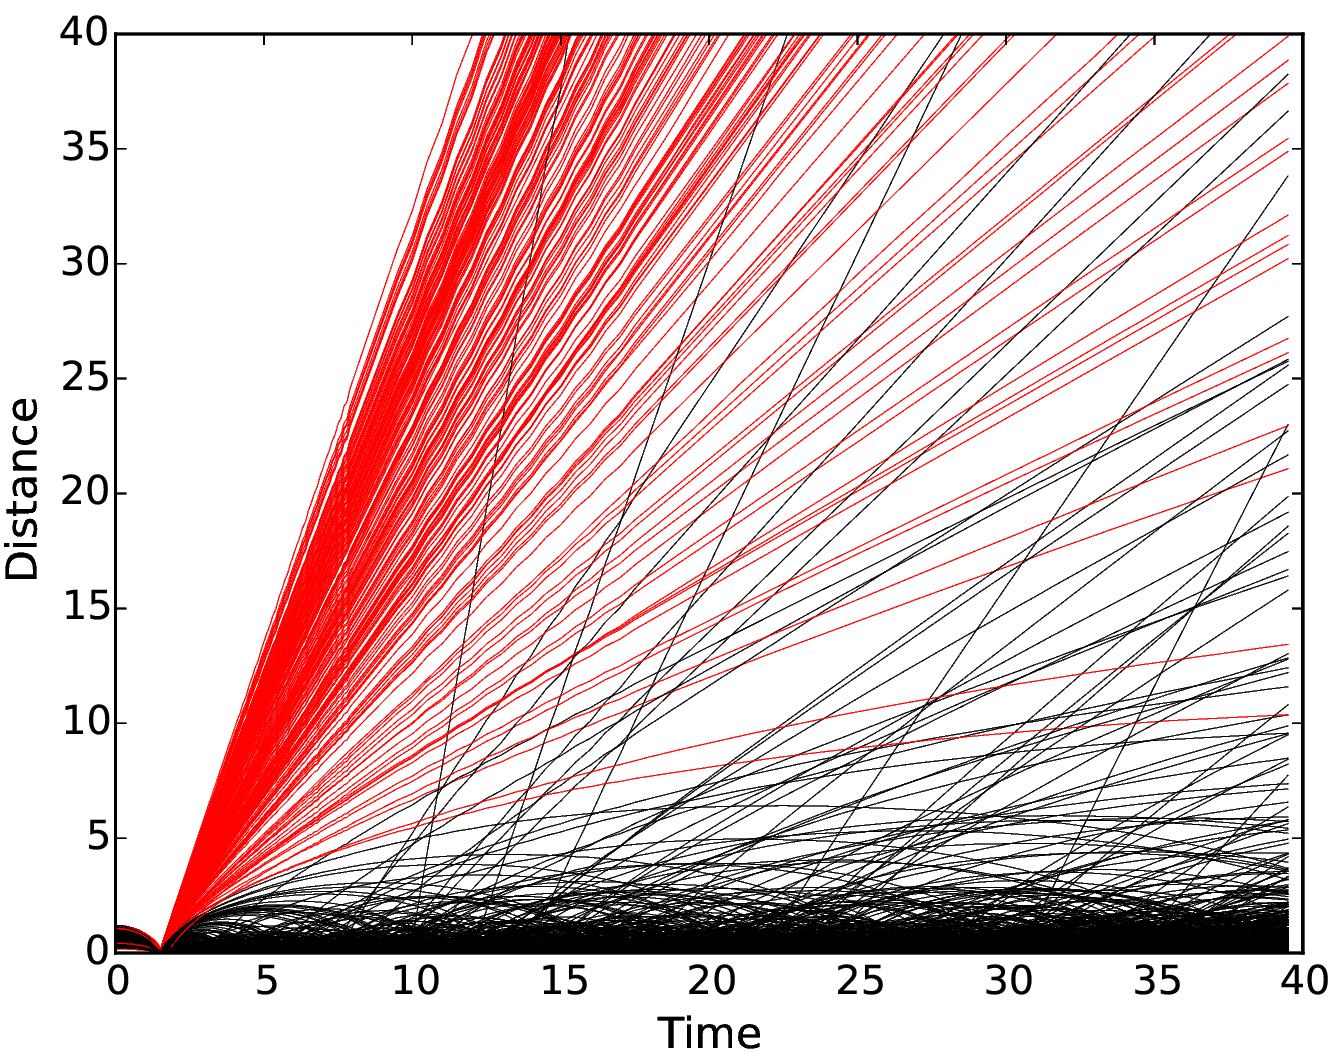
\includegraphics[width=0.7\textwidth]{Figures/3_DistOrigin}
\caption[Distance to origin over time for escapers and bound stars]{Distance to origin for 750 stars from run Ru20 (see Table~\ref{Tab:2_models}). Red lines show the trajectory of stars that are considered ejected according to our criterion.}
\label{Fig:3_DistOrigin}
\end{center}
\end{figure}



  
\section{Collapse and virialisation}
\label{Sec:Collapse}


The constant diffusion of kinetic energy by two-body interaction means that no stellar system ever reaches a steady equilibrium. However we can contrast the time-evolution of two configurations and draw conclusions about their observable properties. 







\begin{figure}
\begin{center}
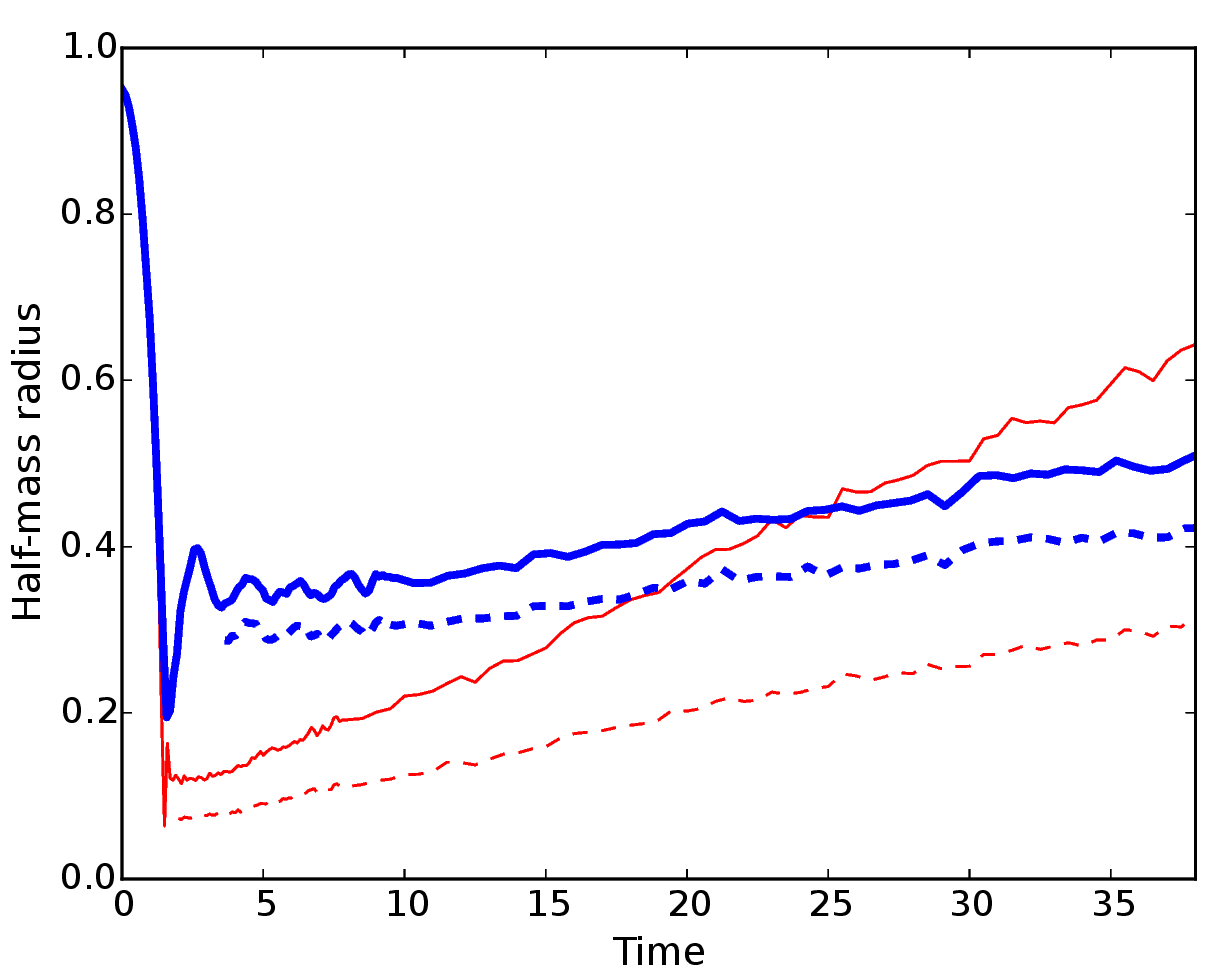
\includegraphics[width=0.7\textwidth]{Figures/3_Rhm_global}
\caption[Half-mass radius as function of time for both HL fragmented and uniform model]{Half-mass radius as function of time for two systems undergoing collapse~: a uniform-density sphere, Ru20, as the thin red solid curve, and a clumpy Hubble model, Rh20, as the thick blue solid curve. Half-mass radii are in H.u, as well as the time axis, where $t_{Henon} = 1 {\rm unit} =  0.13 \Myr$. Dashed lines are the half-mass radii of the same systems for the same systems but including only the bound stars.}
\label{Fig:3_Rhm_global}
\end{center}
\end{figure}




With this in mind  we turn to Fig.~\ref{Fig:3_Rhm_global} in which we show the evolution of the half-mass radius for the cold uniform model (labeled Ru20; thin red curve), and the Hubble model (labeled Rh20; thick blue curve). Both systems have the same bounding radius initially, contract to a small radius when $t \simeq 1.4 $ units and then rebound at time $t \simeq 2 $ units. When all the stars are included in the calculation for $r_h$, we find that the radius increases at near-constant speed after the collapse. That trend does not appear to be slowing down which indicates that a fraction of the stars are escaping. The first batch of escapers is driven by the violent relaxation, however the trend continues beyond $ t = 25$ units, corresponding to $t > t_{ms}$ which implies two-body scattering and effective energy exchange between the stars. Note how the uniform model has a much deeper collapse and rebounds much more violently (as was also seen on Fig.~\ref{Fig:3_collapse}) shedding a fraction twice as large of its stars:
%
%\begin{table}
\begin{center}
%\caption{Number of initially ejected stars in two collapse calculations} \label{tab:Ejectedstars}
\begin{tabular}{lrr}
Run & Ejected stars & Ejected mass  \\
\hline
Ru20  &  4227 & 27\% \\
Rh20  &  1932 & 12\% \\
%\hline
\end{tabular}
\end{center}
%\end{table}




The half-mass radius $R_h$ increases steadily in both models, from the bounce at $t \approx 2$, until the end of the simulation (values in H.u):  
\begin{center}
\begin{tabular}{lllrr}
% & Deepest (t=2) & t=40  \\
%\hline
$R_h$ Uniform & 0.11 &  $\rightarrow$ & 0.63 & ($\times 5$); \\
$R_h$ Hubble & 0.34  &  $\rightarrow$ & 0.49 & ($\times 1.4$). \\
%\hline
\end{tabular}\\
\end{center}

%
% from $ r_h \sim 0.11$ pc immediately after the collapse, to $r_h \sim 0.63$ pc at the end of the run, or a multiplicative factor $\approx 5$. In contrast, the Hubble run drops to $r_h \approx 0.34$ pc and rises over time to $r_h \approx  0.49$ pc (factor of $\approx 1.4$). 
Clearly the gentler collapse of the fragmented model has led to a more extended post-collapse configuration and reduced two-body evolution. Observe how the uniform model Ru20 is ejecting more stars than the Hubble model: if we repeat the calculation for the Hubble run Rh20 but now include only the bound stars, the curve of $R_h$ obtained and shown as dash is shifted down but keeps essentially the same slope $\approx  0.004$. By contrast, the calculation for the bound stars of run Ru20 yields a much shallower slope than for the whole system: the slope drops from 0.015 to about 0.007. Irrespective of how the half-mass radius is calculated, the conclusion remains the same and agrees overall with the remark by \cite{Caputo2014} that boosting the kinetic energy of the collapsing initial configuration softens the collapse~; this was shown in a different context by \cite{Theis1999} and confirms these older findings.  Here, the fragmented model has non-zero kinetic energy due to the clumps internal motion. The important new feature brought by the fragmented initial conditions is that the {\it mass profile} of the virialised configuration evolves much less over time in comparison. 

%%%%%%%%%%%%%%%%%%%


\begin{figure}
\begin{center}
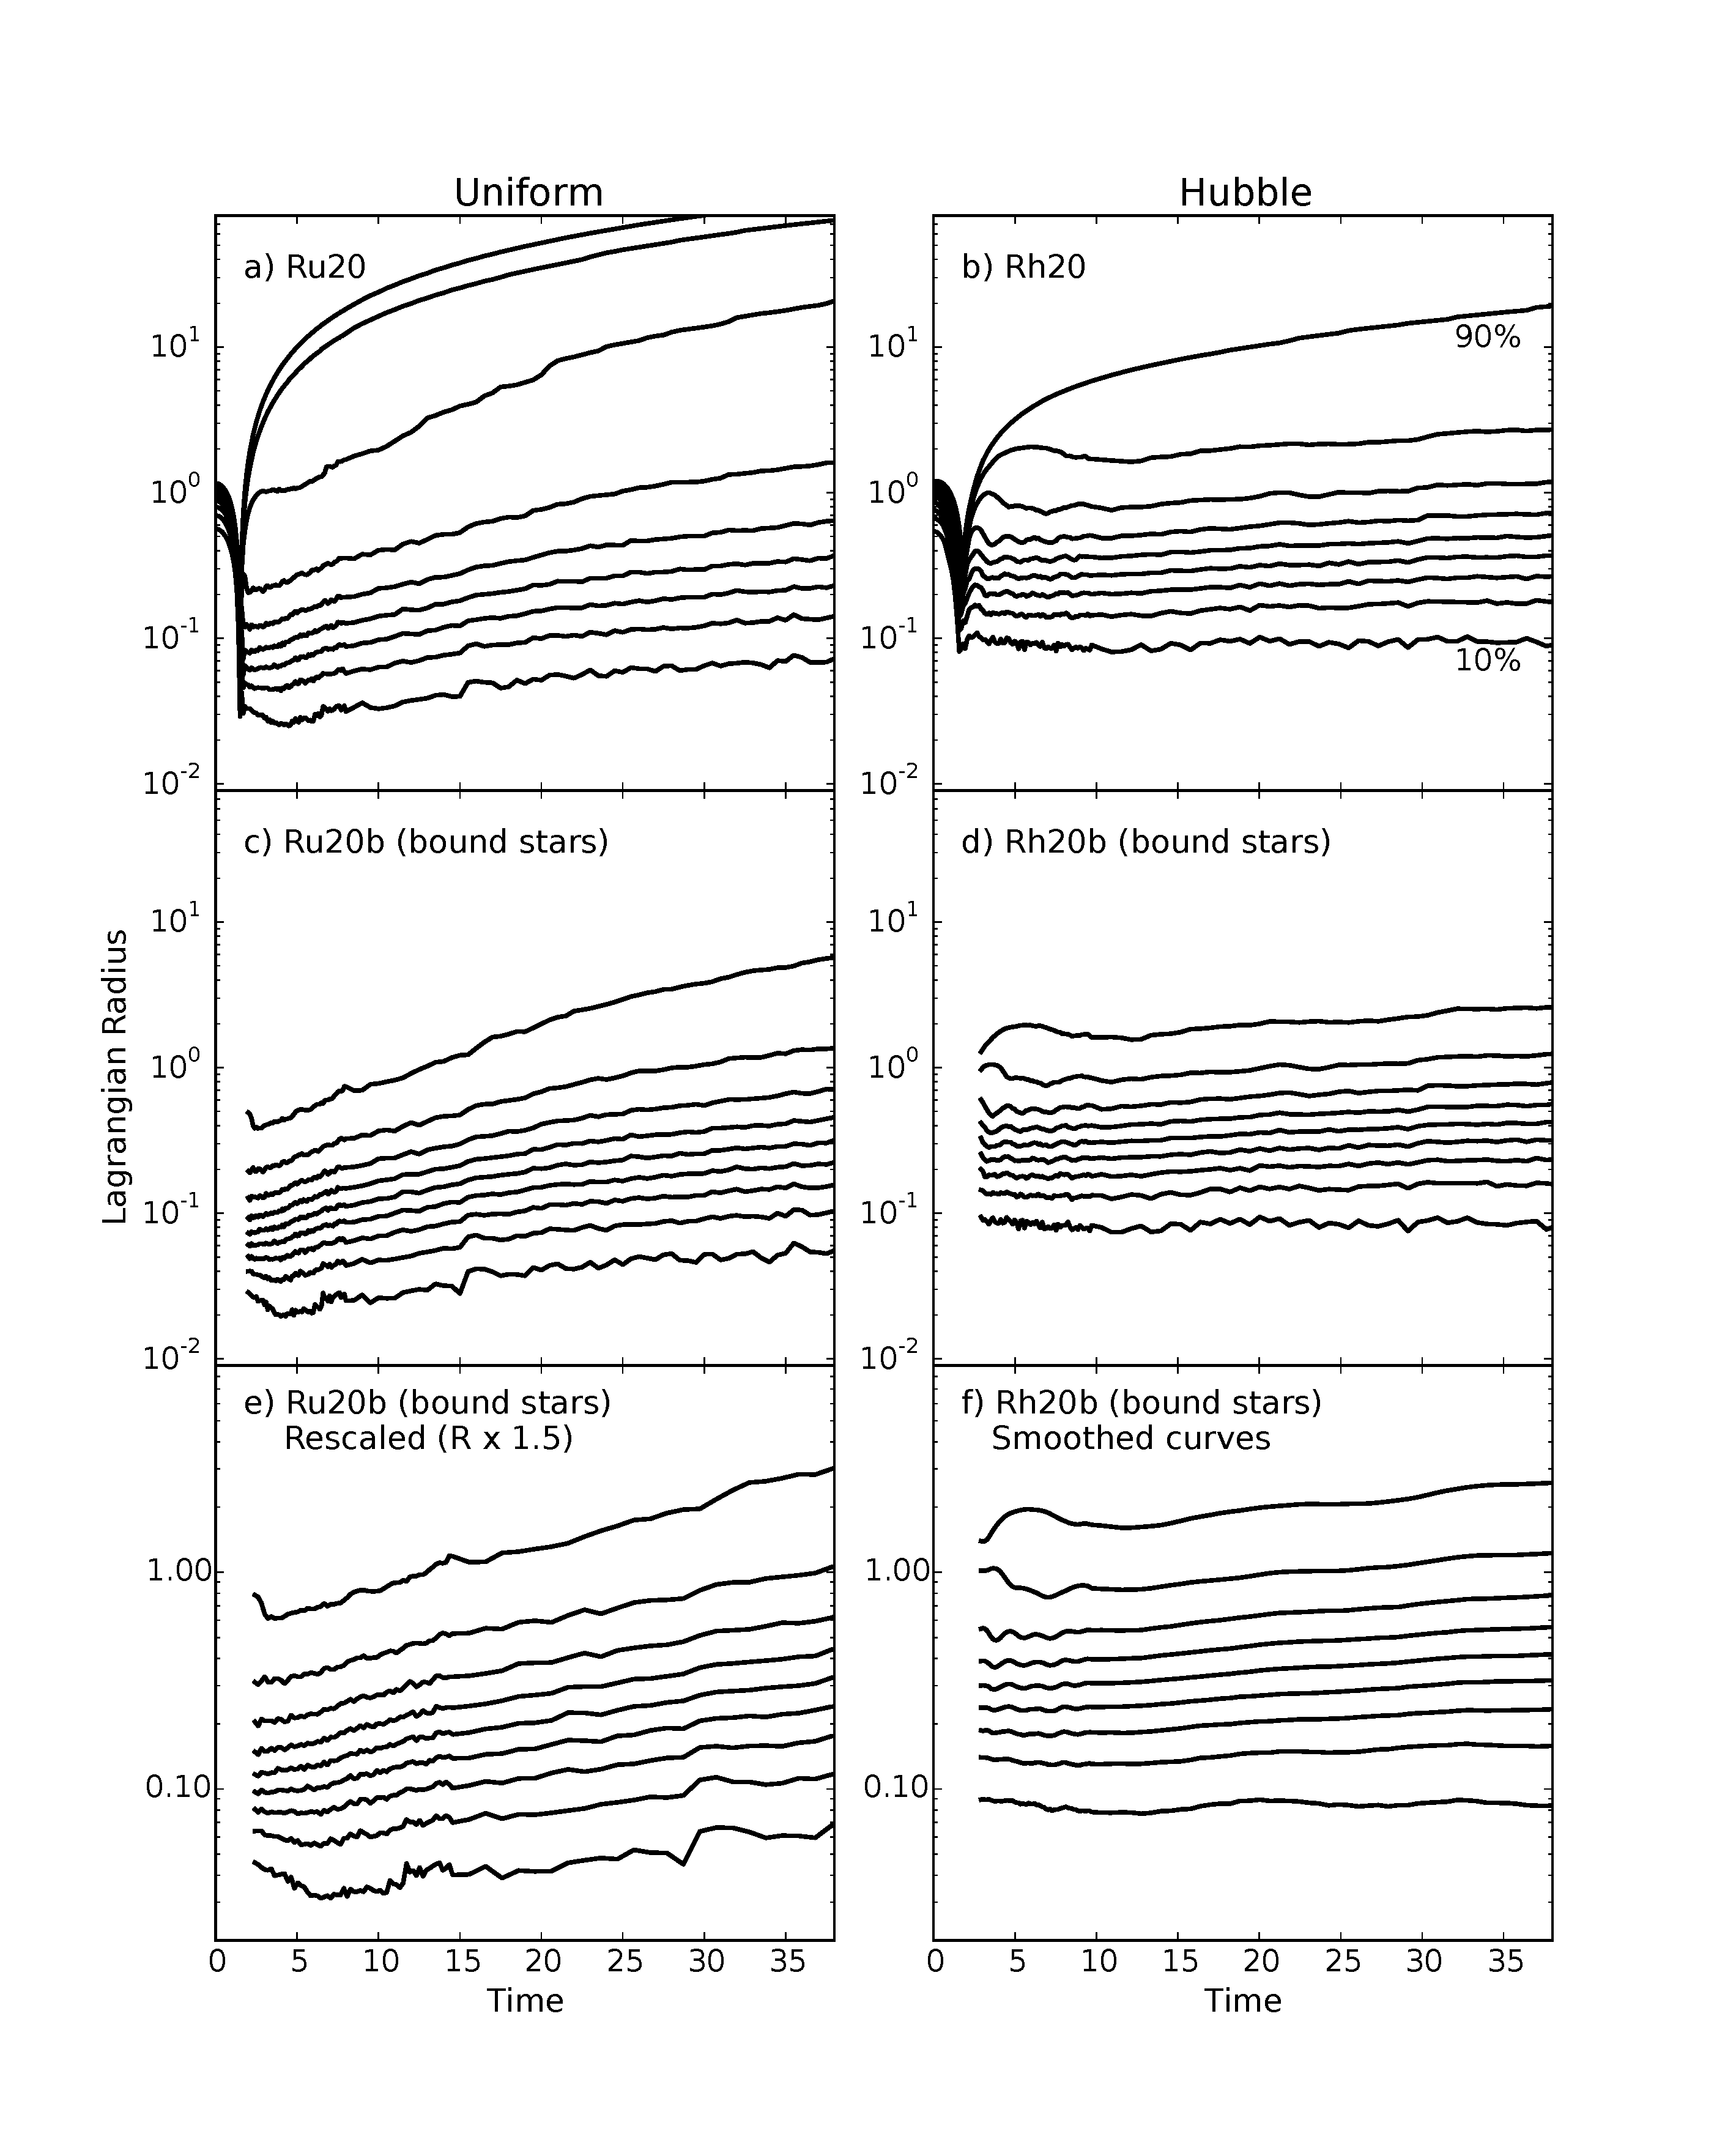
\includegraphics[width=\textwidth]{Figures/3_Lagr_radius}
\caption[Ten-percentile Lagrangian radii over time for HL fragmented and uniform models]{The ten-percentile mass radii (10\% to 90\%) as function of time. Radii and time axis are in H.u, with $t_\Hen = 1 {\rm unit} =  0.13 \Myr$. Left panels show the Uniform model and right panels show the Hubble fragmented models. Panels a and b show the evolution of the whole systems, while panels c and d show the same radii computed for the bound stars only. Panel e shows the Uniform bound model (Ru20b) for which radius and time were rescaled to compensate the difference of initial kinetic energy (see text for details). Panel f shows the same information as panel d with smoothed data. 10\% and 90\% radii are labelled in the top right panel.
%For both, the bottom panel show the bounded systems, with "b" appended to the name,  from which the ejected stars from the initial collapse were removed.
}
\label{Fig:3_Lagr_radius}
\end{center}
\end{figure}


At the bounce, the half-mass radius of the Hubble model is $\approx 4$ times larger than that of the initially uniform sphere at rest (Fig.~\ref{Fig:3_Rhm_global}). The half-mass radii overlap at time $t \approx 15~$H.u. (solid curves) or $t \approx 50~$H.u. (dashed curves). Is the same trend applicable to all Lagrangian radii ? To answer this question we plot on Fig.~\ref{Fig:3_Lagr_radius} the ten-percentile mass radii for the two models. The results are displayed for the two situations including all the stars (top row) or bound stars only (middle row). 

It is striking that the curves show very little evolution at all mass fractions for the case of the Hubble model (see right-hand panels on the figure), whereas all mass shells either contract or expand in time for the uniform one. We have noted how this model should undergo two-body relaxation on a time-scale of $t \approx 320~$H.u. while the innermost 10\% mass shell shows an  indication of \textit{core-collapse} at $t \simeq 5~$H.u.. This is due to the presence of a mass spectrum, the time-scale for core-collapse should be closer to the mass-segregation time-scale,  $t \simeq 25~$H.u.. The remaining difference can be attributed to the smaller total mass (due to the ejecta) and the various assumptions made in section~\ref{Sec:3_Scaling}.

We note here that the two sets of curves reach very similar values at the end of the calculations ($t = 40\, H.u$). A key difference between the two models, therefore, is that the final configuration of the Hubble model is almost identical to what it was at the bounce ; the same simply does not hold in the case of a uniform-density collapse. Furthermore, the Hubble calculation shows no hint of two-body relaxation or core-collapse.
% This raises the possibility that the system properties in the final configuration remain better correlated with those at the on-set of (global) collapse (we return to this point in \S7).

\cite{Caputo2014} and \cite{Theis1999} noted how a non-zero amount of kinetic energy in the {\it initial} configuration alters the  depth of the bounce during collapse. The ratio of half-mass radius at the bounce, to its initial value, is then
\begin{equation}
\frac{R_h}{R_{h,0}} \simeq Q_0 + N^{-1/3}
\end{equation} 
 where $Q_0$ is the virial ratio of the initial configuration \citep[see][Fig.5]{Caputo2014}. We computed the kinetic energy of the  Hubble configuration and found that the internal motion of the clumps means that $Q_0 (Hubble) \simeq 0.02$ for a Salpeter mass function with upper truncation value of $20 \Mo$. With $N = 15k$ stars, the ratio $R_h/R_{h,0} \simeq 0.041$ when $Q_0 = 0$ shifts to $R_h/R_{h,0} \simeq 0.061$ when $Q_o = 0.02$, or a factor close to 1.5. To account for the difference in kinetic energy of the initial configurations, we may therefore rescale the uniform model such that positions are  $ \times 1.5$ and the time unit is $\times (1.5)^{3/2} \simeq 1.84$.
 
  The new configuration would evolve in time in exactly the same way after mapping positions and time to their rescaled values. The result is shown as the bottom row on Fig.~\ref{Fig:3_Lagr_radius}.  Note that we  have blown up the vertical axis to ease comparison between uniform and Hubble models with bound stars only included. The rescaled uniform model is now slightly more extended than before, but overall the final two configurations (at $t = 40~$H.u.) are as close as before rescaling. This demonstrates that  the outcome of the uniform collapse and its comparison with the Hubble model is not sensitive to a small amount of initial kinetic energy. We note that while the ratio $Q_0$ is a free parameter in many setups for collapse calculations, that parameter is fixed internally in the Hubble approach. 










\section{Global mass segregation}
\label{Sec:Segregation} 


To investigate the state of mass segregation in our models, we follow the analysis of \cite{Caputo2014}. The masses are sorted by decreasing values, then subdivided into ten equal-mass bins. This means that the first bin contains the most massive stars. The number of stars in each bin increases as we shift to the following bins, since their mean mass {\it de}creases, and so on until we have binned all the stars. The half-mass radius $R_h$ computed for each bin is then plotted as function of time. In this way the mass segregation unfolds over time: if the stars were not segregated by mass, all radii $R_h$ would overlap. If two sub-populations share the same spatial distribution, their respective $R_h$ will overlap.


\begin{figure}
\begin{center}
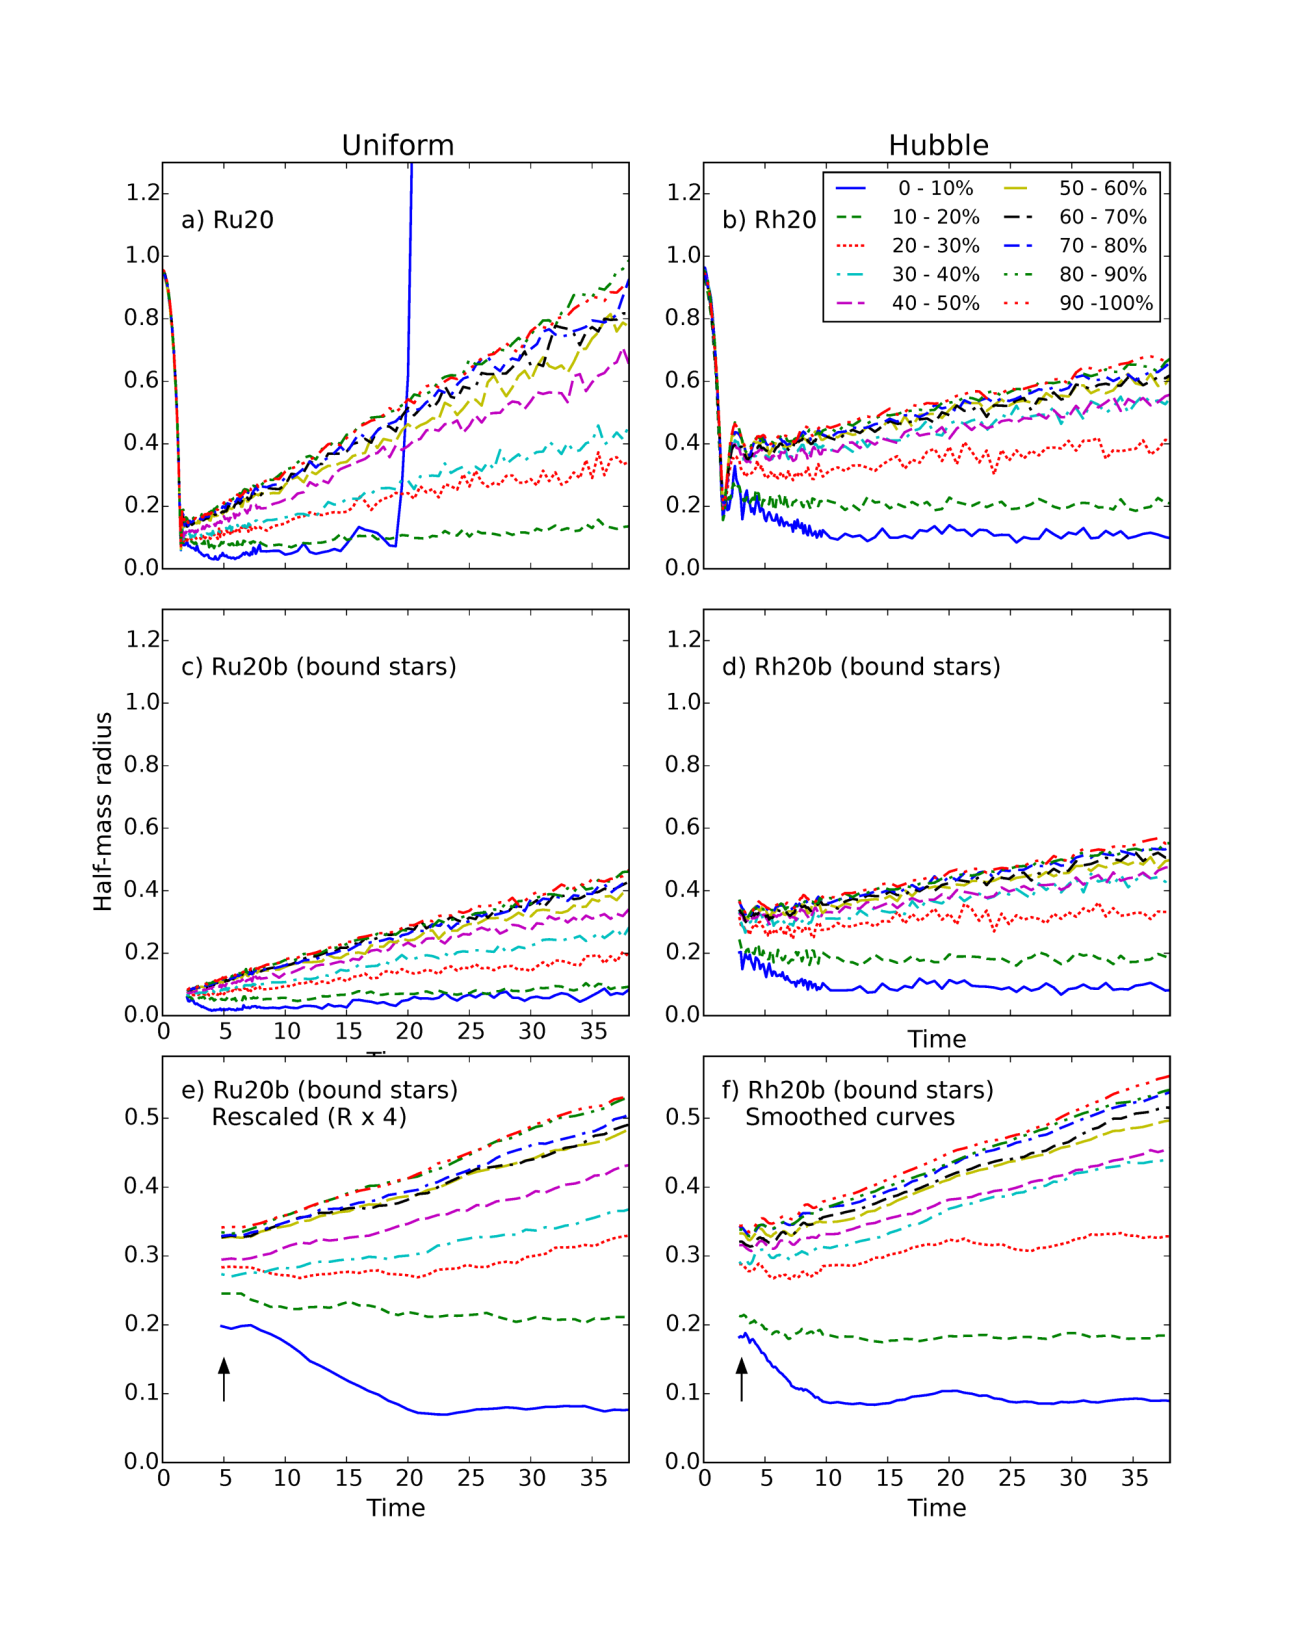
\includegraphics[width=\textwidth,clip=true]{Figures/3_Rhm_segr}
\caption[Mass segregation: half-mass radii over time for mass-selected stars]{Half-mass radii of stars selected by mass as function of time. Each bin identified with 0-10\%, 10-20\% .. 90-100\%, contains ten percent of the total system mass. The stars were sorted by mass in decreasing order, and used to fill each ten-percent mass bin in order. Hence the first ten-percentile contains the most massive stars, the next ten-percentile the second group of massive stars, and so on until the 90-percent bin which contains the least massive stars in the model and is the most populated. Half-mass radius and time are in H.u, with $t_{Henon} = 1\,unit = 0.13 \Myr$. Left panels show the evolution of the Uniform model (Ru20, Ru20b) and right panels do the same for the Hubble model (Rh20, Rh20b). The organization of panels follows the same layout than figure~\ref{Fig:3_Lagr_radius} with a different factor for the rescaling of the uniform system. }
\label{Fig:3_Rhm_segr}
\end{center}
\end{figure}

Figure \ref{Fig:3_Rhm_segr} graphs the results for initially uniform-density and fragmented Hubble models. The layout of the figure is the same as for Fig.~\ref{Fig:3_Lagr_radius}. The violent relaxation phase leads to mass loss for both models and the much more rapid expansion of the half-mass radii of low-mass stars is an indication that most escapers have a lower value of mass.

 Fig.~\ref{Fig:3_Rhm_segr}(c) and (d) graphs $R_h$ for the bound stars of each sub-population. Clearly the initially uniform-density model is more compact early on, but note how the heavy stars sink rapidly to the centre, more so than for the case of the Hubble model. The spread of half-mass radii increases with time for both models, however two-body relaxation in the uniform-collapse calculation is much stronger, so that by the end of the simulations the half-mass radii of the low-mass stars of the respective models are essentially identical. 
 
 Since the low-mass stars carry the bulk of the mass, that means that the two models achieve the same or similar mean surface density by the end of the run. At that time, the heavy stars in the uniform-collapse calculation are clearly more concentrated than in the Hubble run (compare the radii out to $\sim 40\%$ most massive stars). A direct consequence of this is that the {\it color} gradients of the core region of a cluster are much reduced when the assembly history proceeds hierarchically, in comparison with the monolithic collapse. It will be interesting and possibly important in future to compare such models with actual data for young clusters.

Another interesting remark is that the kinematics of the stars within the {\it system} half-mass radius are much different between the two models. For the Hubble calculation, the system half-mass radius, $ \approx 0.43 $ H.u, at $t = 40$ (cf. Fig.\ref{Fig:3_Rhm_segr}d) coincides with the half-mass radius of the $30-40\%$ bin stellar sub-population. All bins up to that range show little or no time-evolution, around the end of the run, which we interpret as efficient retention of these stars by the relaxed cluster. In the case of the uniform-collapse run, the system half-mass radius reaches $\approx 0.33$ H.u., which is significantly larger than the radius for the $30-40\%$ stellar sub-population. For that model, only the bins $0-10\%$ and $10-20\%$ are flat, and all the others increase almost linearly with time. Thus a fair fraction of bright stars deep in the cluster show systematic {\it outward streaming} motion, along with low-mass ones. This brings up the possibility to measure this signature motion through relatively bright stars, originating well inside the cluster half-mass radius. Recall that only post-bounce bound stars where selected to compute $R_h$ on Fig.~\ref{Fig:3_Rhm_segr}(c) and (d) ; the expansion is therefore not driven by escapers (e.g., Fig.~\ref{Fig:3_Rhm_segr}a), but rather through two-body relaxation. On the down side the bright tracers would be short-lived, and this may prove a strong constraint for observational detection.


Given the early dynamical evolution associated with substructured stellar clusters, some observed dense objects may yet be out of equilibrium. We wish to investigate the out-of-equilibrium state of our models just after the collapse. To ease the comparison between the two systems, the same rescaling procedure as for Fig~\ref{Fig:3_Lagr_radius} was applied to the uniform model, only this time the scaling was chosen so that the two clusters have comparable densities after the bounce. Lengths were multiplied by $4$; the time-axis is then scaled up by a factor $(4)^{3/2} = 8$. The result can be seen in panel (e); panel (f) shows a smoothed and zoomed in Hubble model for comparison.



\begin{table}
\caption{Values of half-mass radii and their ratio to that of the most massive stars. The mass categories are labelled X\%-X+10\%, with the percent symbol ommitted for brevity. The results are for the rescaled bound uniform model (rescaled Ru20b) and the bound Hubble model (Rh20b), after the collapse, and before dynamical mass segregation sets in.} \label{Tab:RhmVal}
\begin{center}
\begin{tabular}{l|llllllllll}
Uniform (\%) & 0-10 & 10-20 & 20-30 & 30-40 & 40-50 & 50-60 & 60-70 & 70-80 & 80-90 & 90-100 \\
\hline
Radius   & 0.20 & 0.245 & 0.282 & 0.273 & 0.294 & 0.325 & 0.326 &  0.328 & 0.335 & 0.340 \\
Ratio    & 1 & 1.23 & 1.41 & 1.37 & 1.47  & 1.63 & 1.63 &  1.64 & 1.68 & 1.70 \\

\hline
Hubble (\%) & 0-10 & 10-20 & 20-30 & 30-40 & 40-50 & 50-60 & 60-70 & 70-80 & 80-90 & 90-100 \\
\hline
Radius  &  0.18 & 0.21 & 0.286 & 0.293 & 0.316 & 0.321 & 0.333 & 0.338 & 0.342 & 0.344 \\
 Ratio       & 1 & 1.16 & 1.58 & 1.63 & 1.76  & 1.78  & 1.85 &  1.88 & 1.90 &  1.91 \\
\end{tabular}
\end{center}
\end{table}


%\begin{tabular}{l|llllllllll}
%Uniform  & 0-10\% & 10-20\% & 20-30\% & 30-40\% & 40-50\% & 50-60\% & 60-70\% & 70-80\% & 80-90\% & 90-100\% \\
%\hline
%Radius   & 0.20 & 0.245 & 0.282 & 0.273 & 0.294 & 0.325 & 0.326 &  0.328 & 0.335 & 0.340 \\
%Ratio    & 1.0 & 1.23 & 1.41 & 1.37 & 1.47  & 1.63 & 1.63 &  1.64 & 1.68 & 1.70 \\
%
%\hline
%Hubble  & 0-10\% & 10-20\% & 20-30\% & 30-40\% & 40-50\% & 50-60\% & 60-70\% & 70-80\% & 80-90\% & 90-100\% \\
%\hline
%Radius  &  0.18 & 0.21 & 0.286 & 0.293 & 0.316 & 0.321 & 0.333 & 0.338 & 0.342 & 0.344 \\
% Ratio       & 1.00 & 1.16 & 1.58 & 1.63 & 1.76  & 1.78  & 1.85 &  1.88 & 1.90 &  1.91 \\
%\end{tabular}


We compare the values of the different half-mass radii of the various population before the dynamical mass segregation sets in. This process is clearly visible as the drop of the half-mass radius of the most massive stars during the evolution. We are interested in the segregation which originates from the collapse and is present before this dynamical evolution. Table~\ref{Tab:RhmVal} sums up the values of the half-mass radii taken at $t\sim5$ for both models, both corresponding to the same unevolved post-collapse state (see arrows on panels e and f on Fig~\ref{Fig:3_Rhm_segr}). With on the order of $\sim 100$ stars per bin or more, one estimates roughly a ten-percent standard deviation from random sampling. To measure the \textit{relative} segregation between populations, the table also lists the ratios of each half-mass radius to the one for the most massive stars. 

Both models appear mass segregated (since these ratios are significantly greater than unity). The Hubble model is more segregated, on the whole, albeit in a different way compared to the uniform model. The segregation in that one is more regular and spreads over more mass bins. In the Hubble model, the segregation is much enhanced for the first two mass bins. Such differences in the degree and nature of segregation can be explained by the clumps structure before the collapse. We showed in section \ref{Sec:2_ClumpSegregation} that the clumps were mass segregated with their most massive members being preferentially located at their center. The low membership and mass of most clumps implies that segregation mostly affects the very top of the stellar mass function. This segregation, predominant among massive stars, is then found in the resulting centrally concentrated system, after the collapse, and visible on Fig.~\ref{Fig:3_Rhm_segr}. 

The inheritance of mass segregation was studied by \cite{McMillan2007} for the case of merging Plummer spheres. \cite{Allison2010} furthermore showed that mass segregation in the system as a whole is enhanced for more filamentary  fractal initial conditions (lower dimension, $D$ ; see their Fig. 5). Here our results confirm this observation. Mass segregation is a sensitive function of the initial clumpiness of the system and has immediate bearing on the dynamics of the virialised configuration, since all massive stars are more concentrated in the core.


\section{Concluding remarks}


We have followed \HubLem fragmented models throughout collapse and subsequent dynamical evolution, and compared their structure and mass segregation to cold uniform models. We found fragmented models undergo a softer, shallower collapse than uniform models, due to their irregular spatial distribution and internal kinetic energy. Uniform models eject more than twice as much stars from the system at the bounce due to this deeper collapse and virialize with a 4 times smaller half-mass radius. This high concentration enhances two-body evolution and the uniform systems expand faster than the Hubble models, even when excluding the ejected stars from the system. Interestingly, after 40 H.u, or 6 Myr, both systems achieve approximately the same density and distribution.

Both uniform and fragmented models develop mass-segregation over time, with the low-mass stars being preferentially ejected or diluted. In the end of the simulation, the uniform systems appear slightly more mass-segregated due to their denser configuration and enhanced two-body evolution. However, just after collapse, \HubLem models exhibit a mass segregation mainly affecting the most massive stars. This characteristic is preserved throughout evolution while the segregation seen in uniform models is more spread out in the mass function. This is  a signature of the hierarchical formation, as this ``top-focused" segregation developed in small clumps and was inherited by the whole system. This would enhance colour gradient in the core of real clusters, opening the way for an observational criteria to assess the formation scenario of very young relaxed clusters.






   

    \part{Binary stars in substructured clusters}
    
\chapter{Introduction to binaries}

In the second part of this thesis we turn to binary stars and their relation to star clusters. 

\paragraph*{}
Binary stars are crucial to understand the evolution of star clusters for a variety of reasons. They can be a reservoir of energy, supporting the core of a cluster against collapse by giving away their internal energy to perturbers, heating the system and possibly ejecting stars, affecting its global evolution and stopping core collapse (e.g \citealt{Heggie1992}).

The statistical properties of binary star populations in dense stellar associations in particular may shed light on the discovery of multiple star-formation episodes in rich stellar clusters \citep{anderson2009}. For instance, binary stars enhance strong dynamical interactions which in turn may speed-up evolution off the main sequence and so boost enrichment of the ISM through winds (e.g., \citealt{Tailo2015}). Tight binaries of short-lived massive stars may evolve to produce exotic stellar remnants including black hole progenitors \citep{bacon1996,davies2009}. Blue stragglers, abnormally hot stars for the age of their host clusters, are thought to form in binary mergers, making them a dynamical record of the past binary population and dynamical state of the cluster \citep{Knigge2009}.

Finally, accurate knowledge of binary populations in stellar clusters enable good estimation of their dynamical mass, as the integrated velocity dispersion is largely biased by the binaries internal motions, see \cite{Rubenstein1997}.

In this short introduction to binaries, we define a binary system, describe a statistical measure for a binary population, then introduce the observational and numerical work on binary population both in the field and in clusters.


\section{What is a binary star ?}

When two massive bodies of mass $m_1$ and $m_2$ interact gravitationally, they can have different types of trajectory depending on their total energy

\begin{equation}
E = E_k + E_p = \frac{1}{2} m_1 v_1^2 + \frac{1}{2} m_2 v_2^2  - \frac{G m_1 m_2}{\| \bold{r_1} - \bold{r_2}\| }.
\end{equation}

%\begin{itemize}
%\item[$\bold{E>0}$], the system is unbound, the bodies follow hyperbolic trajectories. They have a distance of closer approach then move away from each other forever.
%\item[$\bold{E=0}$], the system is marginally unbound, the bodies follow parabolic trajectories.
%\item[$\bold{E<0}$], the system is bound, the bodies have stable elliptical orbits around each others.
%\end{itemize}

If $E<0$, they are bound and locked in a binary system. Such systems are characterised by their semi-major axis $a$, their eccentricity $e$, their period $p$, their total mass $m_t = m_1 + m_2$, mass ratio $q = m_2/m_1$ with $m_1$ being the primary, more massive than $m_2$.
Mass, period and semi-major axis are related by Kepler's third law

\begin{equation}
\frac{G m_t}{4\pi^2} =  \frac{a^3}{p^2}.
\end{equation}

Interestingly, expressed in AU, $\Mo$ and years, $G \simeq 4 \pi^2$, thus the law can be written

\begin{equation}
\left( \frac{m_t}{1 \Mo} \right) \simeq \left( \frac{p}{1 \textrm{yr}} \right) \left( \frac{a}{1 \textrm{AU}} \right)^3 .
\end{equation}



\begin{figure}
\center
    \centering
    \begin{subfigure}[b]{0.48\textwidth}
    	\centering
        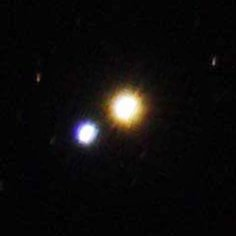
\includegraphics[width=0.6\textwidth]{Figures/0_albireo.jpg}
        \caption{Albireo ($\beta$ Cygni)}
        \label{Fig:0_binary_1}
    \end{subfigure}
    ~~
    \begin{subfigure}[b]{0.48\textwidth}
    	\centering
        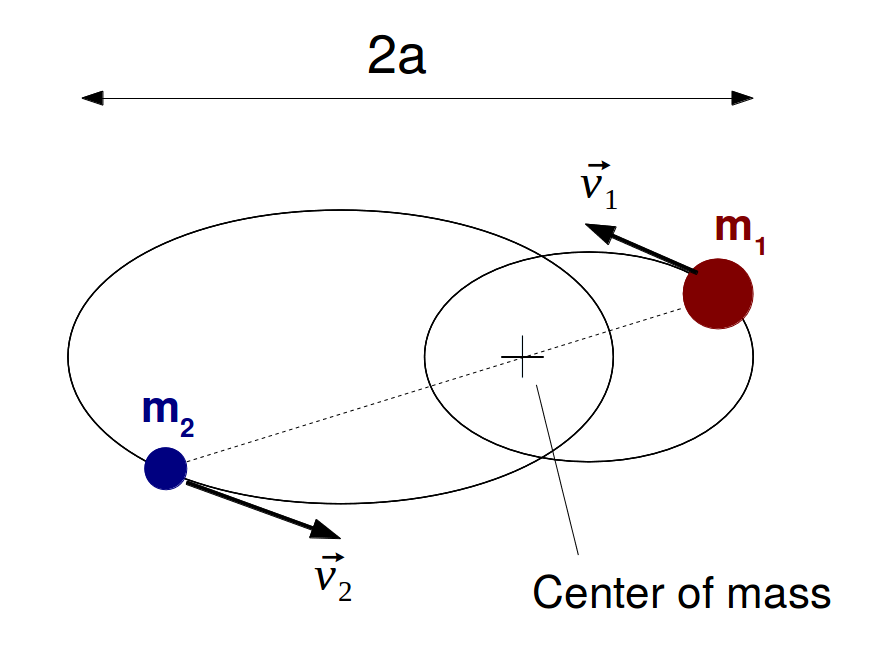
\includegraphics[width=0.93\textwidth]{Figures/0_elliptictrajectories.png}
        \caption{Schematic of a two-body system}
        \label{Fig:0_binary_2}
    \end{subfigure}
\caption{(a) Hubble observation of the binary star Albireo, fifth brightest star in the Cygnus constellation. Albireo A, the red star, is a close binary system itself (not represented on (b) for simplicity). The pair has a period of 213 years and a semi-major axis $a \simeq 66$ AU. }
\label{Fig:0_binary}
\end{figure}





The total energy of the binary can be expressed as a function of $a$, $m_1$, $m_2$:

\begin{equation}
E = - \frac{G m_1 m_2}{2a} 
\end{equation}



\section{Multiplicity fraction}

In a stellar population, a fraction of stars will be found in multiple systems: some  in binaries and some in higher order hierarchies. A hierarchical triple is a stable 3-body bound system, a binary of which one of the component is a binary itself. The same principle applies to quadruple, quintuple, etc. One of the brightest stars in the night sky, Castor, is a sextuple hierarchical system, with 6 stars in a stable system.

Counting binaries and multiples is not straightforward: do you count triples as two binaries or three stars in a multiple system ? In their SPH simulation paper, \cite{Goodwin2004a} discuss several ways to measure the degree of multiplicity among stars in a system, each of them quantifying different properties, such as companion probability, companion frequency or pairing factor. 

Let  S be the number of single stars, and B, T and Q the number of binary-, triple-, and quadruple systems, respectively. The fraction of multiple stars bound in binaries, triples and quadruples to the total number of multiple plus single stars, is

\begin{equation}
\label{Eq:0_fm} 
f_m = \frac{B + T + Q}{S + B + T + Q}. 
\end{equation}

This measure is used in seminal observationnal papers \citep{DM91,Raghavan2010} and is our adopted choice. As pointed out by \cite{Hubber2005}, $f_m$ in Eq. (\ref{Eq:0_fm}) has several advantages: 1) it  may be  restricted to a given mass $m$, setting  $S_m$ the number of single stars, and $B_m,\, T_m,\, Q_m$  the multiple stars with a primary of that mass;  2)  the multiplicity fraction is observationally robust: when a binary is being reclassified as a triple, or an even higher order multiple system, the fraction does not change. 
 These definitions may be extended to cover a mass range  in a coherent way, by substituting $m \rightarrow \langle m\rangle$, the mean value over the range. This is useful mostly when comparing  systems with different stellar mass functions. 


\section{Observed population}
\label{Sec:0_raghavan}

\begin{figure}
\center
    \centering
    \begin{subfigure}[b]{0.48\textwidth}
    	\centering
        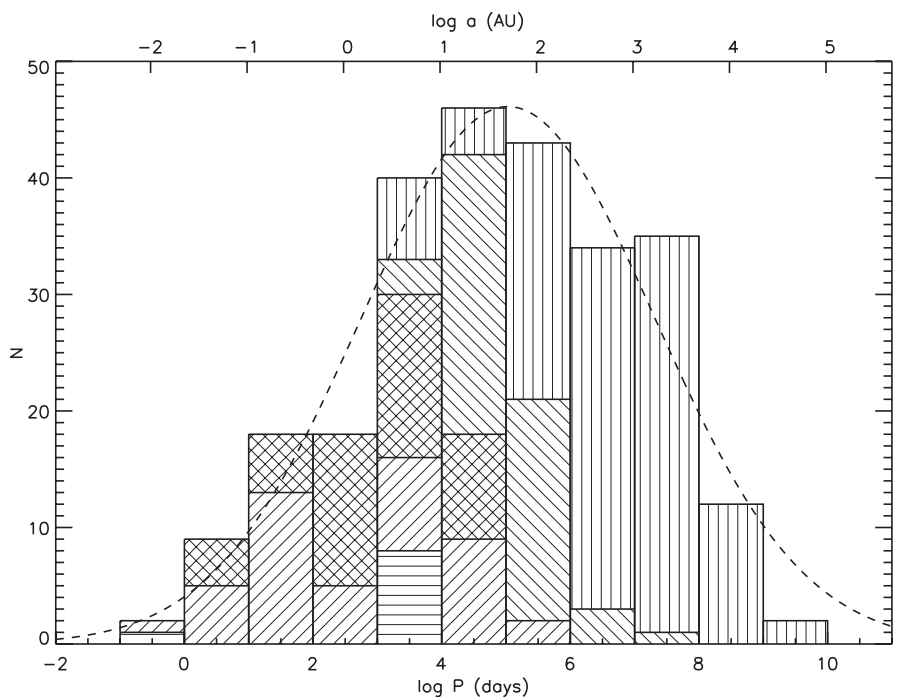
\includegraphics[width=\textwidth]{Figures/0_binperiods.png}
        \caption{Period and semi-major axis distribution}
        \label{Fig:0_binpop_1}
    \end{subfigure}
    ~~
    \begin{subfigure}[b]{0.48\textwidth}
    	\centering
        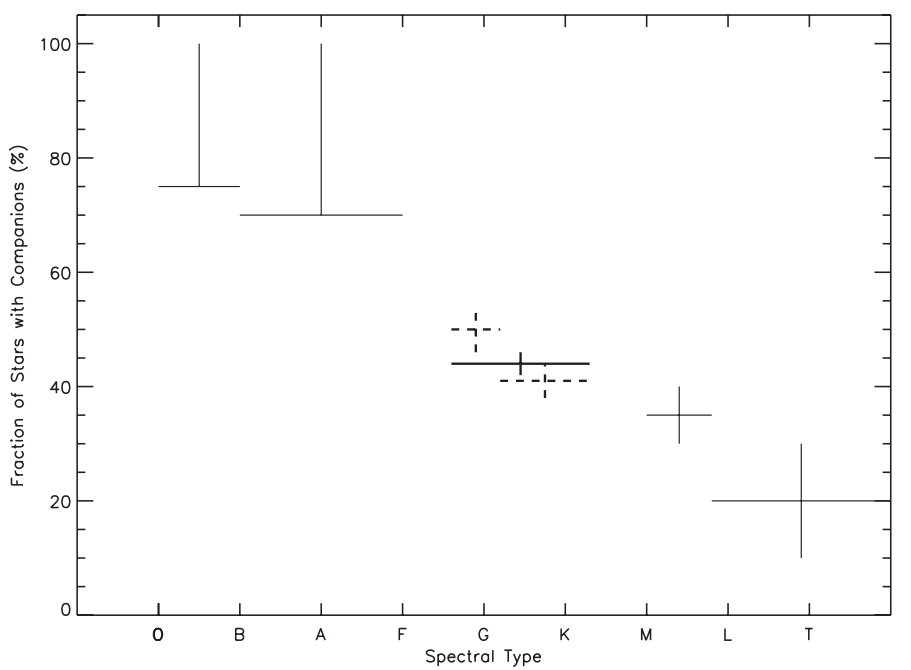
\includegraphics[width=0.97\textwidth]{Figures/0_binfraction.png}
        \caption{Binary fraction vs spectral type}
        \label{Fig:0_binpop_2}
    \end{subfigure}
\caption{(a) shows the observed distribution of period and semi-major axis observed in the field. Different hatchings show different observation techniques: horizontal lines show unobserved companions detected by the proper-motion acceleration of components, positively sloped lines show spectroscopic binaries, negatively sloped lines visual binaries, cross hatching show objects found with both, and vertical lines are objects with common proper motions. (b) was compiled from several surveys, detailed in Fig~\ref{Fig:5_spontaneous_primarymass}. Both figures were extracted from \cite{Raghavan2010}. }
\label{Fig:0_binpopulation}
\end{figure}




A seminal survey of binary solar-type stars in the field was performed by \cite{DM91}. This seminal paper was updated and completed by \cite{Raghavan2010}, who essentially confirmed the main results from the first study. They observed hundreds of F and G main-sequence stars in pairs and derived their binary parameters. The total binary fraction for these stars was found to be $\sim$ 53\% as binaries are quite common in most stellar populations.
  The authors also derived a period distribution, extending from less than a day to more than a Myr. The distribution was consistently well fitted by a log-normal distribution. The period distribution for F and G stars (as well as K and M stars, see \citealt{Fischer1992}) is
\begin{equation}
f( \log{P})\propto \exp \left[ \frac{- ( \log{P} - \mu_{logP})}{ 2 \sigma_{logP}^2} \right],
\end{equation}
with the peak value $\mu_{logP} = 5.03$, about 300 years, and the dispersion $\sigma_{logP} = 	2.28$, the distribution is shown on Fig~\ref{Fig:0_binpop_1}.

\cite{Raghavan2010} also compiled several observational studies of binaries with primaries of various spectral types. High mass stars, types O,B,A, (from 30+ down to 2$\Mo$) have a high multiplicity fraction, about 75\%  while lower mass stars such as M-dwarfs only have 10-30\% multiplicity, see Fig~\ref{Fig:0_binpop_2}. This trend of increasing multiplicity with increasing primary mass is found in many surveys.
Binary surveys are easier in the field due to the very large sample and low stellar density. To perform similar studies in young star clusters is much harder due to source crowding and embedded stars. \cite{Kouwenhoven2007} attempted to characterize the birth binary population in the OB association Scorpius OB2. They found a very high multiplicity fraction, consistent with 100\%, and a period distribution more consistent with a powerlaw than a log-normal distribution. From this survey and others, it is likely that the binary population in clusters undergoes an erosion through dynamical processing, with the field distribution as an end-result.

\section{Simulate binary populations in clusters}

As noted earlier, young clusters are born substructured, then undergo dynamical evolution. The rapid, global  merging of sub-structures would bring together stars at a different stage of their  formation (as in NGC1333, see \citealt{Foster2015}) while at the same time induce a shift from a clumpy Taurus-like profile to a more regular one. A simple but important question is how the internal dynamics of such complex configurations may affect the  characteristics of a population of binary stars. 

Many authors have explored this question through optimised initial conditions \citep{Kroupa2001,Marks2012} or fractal configurations evolved with N-body integrators \citep{Parker2011,Geller2013,Parker2014}. A common feature to all these studies is that the binary fraction drops over time regardless of their components (masses), due e.g. to close star-star encounters or heating from the external galactic tidal field, see Fig~\ref{Fig:0_binsim_1}. It was also shown that wide binaries are, as expected, more prone to destruction than more compact systems, as is illustrated by the evolution of the population seen in Fig~\ref{Fig:0_binsim_2}.

 \cite{Parker2014} pointed out that the distribution of semi-major axes $a$ of the field population is a strong function of the primary's mass: at fixed $a$, low-mass binaries carry less binding energy so the distribution cuts off at shorter separation ($\sim 20 $ AU) compared to that for binaries with a more massive primary ($\sim 300$ AU). Their study of fractal initial conditions show that gravitational dynamics enhances the dissolution of low-mass systems. This then provides a clue to account for the larger relative fraction of heavy stars in binaries, such as seen in a compilation by \cite{Raghavan2010}. 
 
 
\begin{figure}
\center
    \centering
    \begin{subfigure}[b]{0.48\textwidth}
    	\centering
        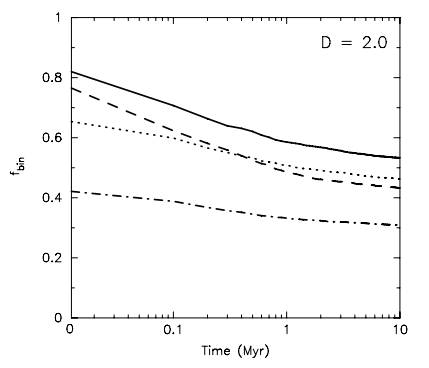
\includegraphics[width=\textwidth]{Figures/0_binfraction_evolution.png}
        \caption{Evolution of total binary fraction}
        \label{Fig:0_binsim_1}
    \end{subfigure}
    ~~
    \begin{subfigure}[b]{0.48\textwidth}
    	\centering
        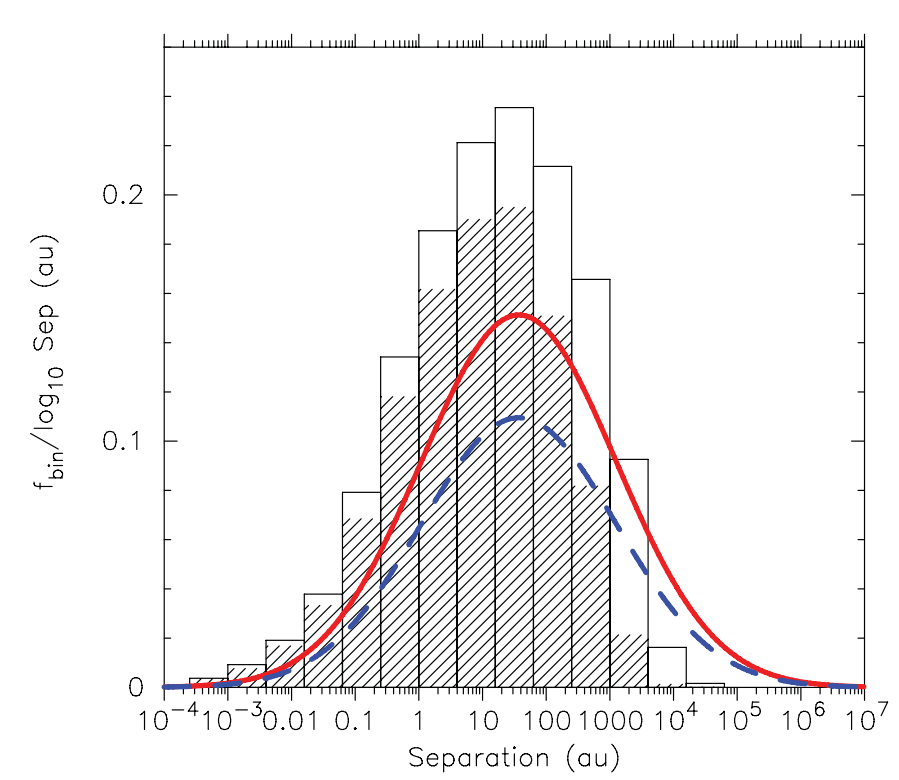
\includegraphics[width=0.97\textwidth]{Figures/0_separation_evolution.png}
        \caption{Evolution of semi-major axis distribution}
        \label{Fig:0_binsim_2}
    \end{subfigure}
\caption{(a): total binary fraction over time in a subvirial fractal system. Corresponding models for the solid, dashed, dot-dashed and dotted are respectively 100\% initial binary fraction with log-normal distribution, 100\% fraction with Kroupa distribution, field-like fraction with log-normal distribution and field and 75\% fraction with log-normal distribution. (b): 100\% initial binary fraction with an initial log-normal distribution (open histogram) and the evolved distribution after 1Myr (hashed histogram). Solid red and dashed blue lines are fits for, respectively, the G-dwarf and M-dwarf populations. Both figures were extracted from \cite{Parker2011}.}
\label{Fig:0_binsimulation}
\end{figure}

 
 
%  We note that hydrodynamical calculations of star formation have found young heavy stars to be preferentially found in dense clumps \citep{Maschberger2010}.
   Furthermore, it is not clear yet whether binary populations should be tailored according to the total system mass because of the limited range of $M \sim 10^2$ to $ \sim 10^3 M_\odot$ of these studies \citep{Kroupa2001,Parker2011,Parker2014}. Recall that the intensity of the tidal field is a prime agent of binary heating.  A trend with mass may be expected on the ground that the drive to equilibrium of more massive systems leads to deeper potential wells (e.g. \citealt{Aarseth1988,Boily2002}). A steep potential will give rise to strong tidal fields which may disrupt bound sub-systems \citep{Boily2004,Renaud2011}. A definitive assesment of this effect is difficult to reach because the results are a strong function of the system initial mass distribution and kinetic energy content \citep{Boily2002,Caputo2014}.
  
  
\paragraph*{}
In the following chapters, we present an algorithm to detect binary stars in N-body simulations. This algorithm is applied to \HubLem fragmented configurations, revealing a spontaneous binary population created by the expansion of the initial uniform sphere. We inject new binaries in the system to follow observed trends in the binary distribution. These systems are then left to collapse, as before, and the binary populations are monitored. We evaluate the influences of cluster membership and stellar density on the processing of binaries in substructured and subvirial systems. We also detail the formation of "extreme" binaries in our simulations, very short and very wide systems, and their dynamical origins.








	
    
\chapter{Detecting and injecting binaries}


In this chapter, we introduce a new algorithm to detect and record binary system in N-body simulations. With this tool, we analyse the spontaneous binary population arising in the \HubLem systems and we describe a binary injection method to complete this population to match the observations.


\minitoc

\section{A new binary detection algorithm}


\subsection{Density comparison}

The study of binary populations in nbody simulations requires an algorithm to detect binary systems and compute their characteristics. The simplest approach is to compute all star-star energies and consider bound pairs as binaries. This records a lot of ephemeral interactions, as n-body dynamics cause transient bound systems. An additional criteria is needed to assess the stability and robustness of a pair as a binary.

\begin{figure}
\begin{center}
\includegraphics[width=0.6\textwidth]{Figures/5_kdtree}
\caption{Illustration of a kdtree for a random two-dimensional distribution (blue dots).}
\label{Fig:5_kdtree}
\end{center}
\end{figure}


We introduce a new algorithm based on the idea of a density threshold: binaries must be denser than their direct environment. Before describing the algorithm, we wish to emphasize the importance of neighbour searches in this kind of study. Be it to obtain bound pairs or to study said pair direct environment, the quick retrieval of neighbours is crucial to an effective algorithm.

The method described here relies on the KD-tree algorithm \citep{numericalrecipes}. While brute-force neighbour searches scale as $\propto N$, as all stars in the system have to be checked as potential neighbours, a KD tree, once built, performs neighbour searches with algorithmic complexity $\propto\log (N)$. The tree is built by sorting particles along one dimension, splitting them at the median, then sorting each branch along another dimension, splitting them again, and so on, cycling over dimensions. A two-dimensionnal example is show on Fig~\ref{Fig:5_kdtree}.





First, binary candidates are identified as negative energy pairs. The semi-major axis of the system is derived from the star motions, then a "binary density" is computed, with $a$ the binary's semi-major axis :
\begin{equation}
 \rho_{binary} = \frac{m_1 + m_2 }{4\pi a^3/3 }\, .
\end{equation}
This is then compared to the local neighbour density, defined as the cumulated mass of a fixed number $N_{nb}$ of neighbours to the pair over the spherical volume reaching to the last neighbour.
\begin{equation}
 \rho_{local} =  \frac{\sum\limits_{i=0}^{N_{nb}} m_i}{ 4 \pi r_{N_{nb}}^3 /3} .
\end{equation}


\begin{figure}
\begin{center}
\includegraphics[width=0.6\textwidth]{Figures/5_neighbours}
\caption{Illustration of the density threshold method. The central blue stars and the red bound neighbour describe a two-body orbit shown on the figure while the green bar indicates the major-axis of the system. This defines the binary density, green sphere, while the local density is defined with the grey stars, the other neighbours. Here, $N_{nb}$ was set to 7. }
\label{Fig:5_neighbours}
\end{center}
\end{figure}




If the density ratio exceeds a threshold $D$, 
\begin{equation}
\label{Eq:density_ratio}
\frac{ \rho_{binary} }{ \rho_{local} } > D,
\end{equation}
the pair is registered as a binary.  Other authors, eg \cite{Parker2009,Lomax2015}, have used close hybrids of the criteria that we have implemented.

Stars can be found to be part of several binaries at once, which happens more often for massive stars as they clear more easily the density threshold. When that happens, the algorithm selects from such connected systems only the pairs exhibiting the lowest (most negative) binding energy.

This method has two free parameters: $N_{nb}$ and $D$. $N_{nb}$ can be set from 6 to 10 neighbours without a substantial impact on the detection. The density ratio is a more critical parameter, as if it is chosen too low, a lot of ephemeral binaries are found, while a high value picks only the closest binaries, ignoring wider, yet stable, systems.



\subsection{Choosing a density ratio}



\begin{figure}
\begin{center}
\includegraphics[width=\textwidth]{Figures/5_sm_ratios}
\caption{Semi-major axis histograms for various value of the density ratio $D$ at t=0 and 10 H.u for a 10k star King model and a binary fraction $f_b =0.3$. The injected log-normal population is shown as a black solid line.}
\label{Fig:5_sm_ratios}
\end{center}
\end{figure}



We wish to find a good compromise value for the critical density ratio $D$ that maximizes the number of detected stable binaries without collecting too much transient system. To do so, we explore the results brought by different values of $D$ in a nbody system containing binaries.

We create a virialized King model with N = 10000 stars and a binary fraction of 0.3. This means there are 2300 binaries and 5400 single stars:
\begin{equation}
f_b = \frac{N_b}{N_s + N_b} = \frac{N_b}{N-N_b} \quad \implies \quad N_b = \frac{f_b}{1+f_b} N = 2300.
\end{equation}
The binaries follow the \cite{Raghavan2010} log-normal distribution introduced in \ref{Sec:0_raghavan}. We let the system run for 10 H.u, or 12 crossing times, and write a snapshot every 0.1 H.u.

The binary detection is ran over all snapshots once per density ratio in the following list:

\begin{center}
\begin{tabular}{l|rrrrrrrrr}
\centering
D  &  2000 & 500 & 150 & 60 & 30 & 10 & 5 & 2 & 1\\ 
\end{tabular}
\end{center}

We show on Fig~\ref{Fig:5_sm_ratios} the semi-major axis distribution retrieved for various $D$ for t=0 and t=10, with the theoretical injected population as a solid black line.



\begin{figure}
\begin{center}
\includegraphics[width=0.9\textwidth]{Figures/5_flickering}
\caption{Visualization of the wide ($a>1000$ AU) binary population in a King model over time. Large upper panel show the evolution of all binaries detected for a density ratio $D=2000$, ordered by time of first detection. Each lower sub-panel show the new binaries detected with the new, lower, value of $D$ compared to the previous one.}
\label{Fig:5_flickering}
\end{center}
\end{figure}

Looking at the left panel, for t=0, we see all density ratios return the same population for $a < 1000$ AU, while for higher separation, there are large variations. $D = 2000$ does not detect semi-major axis larger than 3000 AU, while $D = 1$ detects $\sim$ 30 systems with $a > 10^4$ AU. After 12 crossing times, on right panels, we see the tight detected population didn't change, while all wide populations converged. The highest ratios did not undergo much change, while low ratios saw a large depletion of the population they initially returned. 

 We can say that a very high ratio only detect binaries that are garanteed to resist the dynamical processing and survive, while low ratios detect more fragile systems. How ephemeral are these latter binaries ? To evaluate the different population detected by different ratios, we show on Fig~\ref{Fig:5_flickering} the detailed evolution of the wide, $a>1000$ AU population. The large upper panel show all wide binaries evolution (time on y-axis) for $D=2000$, arranged on the x-axis by time of first detection. Each pixel column represents a binary. The smaller sub panels show, for each density ratio, the history of the binaries this ratio detected that the previous, greater ratio did not. A binary that is detected with $D=2000$ will also be detected for $D=500$ and any other lower value. Fig~\ref{Fig:5_flickering} shows what kind of binaries lowering the ratio progressively brings to the detected population. The color codes the logarithm of the semi-major axis in AU, white means the binary is not detected.

The $D=2000$ population is mainly made of stable, relatively tight binaries. About half the binaries are detected at t=0, while the others dynamically form in the system. Some are destroyed, other widened through interactions as their color bars transitions to a lighter color, sometimes after a "flickering" phase, when the detection goes on and off over successive snapshots. This is due to the binary entering a dynamical interaction with a third star or other binary, making the neighbour density undergoing spikes. This interaction leaves the binary with a weaker bound, thus higher binding energy. 

Looking at the populations brought by lower ratios, we see they are progressively wider and more transient/flickering as the ratio lowers, which is to be expected. $D=1$ only brings very ephemeral pairs, often not lasting more than a single snapshot. All ratios bring their share of transient binaries, but $D=10$ is the last to capture relevant, relatively long-lived pairs.

Extreme values of density ratios bring a large difference in the detection of large binaries, but a moderate value like $D=10$ appears the best compromise to capture the substance of a binary population.










\section{The spontaneous binary population} 




Star-star interactions which take place during the HL expansion phase speed up the internal evolution of small substructures (or, clumps). The global expansion, on the other hand, brings about correlations in phase-space coordinates and the formation of loose binary stars (see Appendix A and \citealt{Kouwenhoven2010,Moeckel2011}). We refer to that population of binary stars as {\it spontaneous} binaries in the following. There is a trade off between the creation of spontaneous binaries, and their destruction / heating when they sit near or inside a clump. Their properties as a sub-population will be addressed statistically through numerical experiments.


\subsection{Binary fraction vs primary mass}
\label{Sub:spontaneous_binaryfractions}

Several studies have found a strong correlation between the binary fraction $f_m$ and the primary mass $m$ of a binary system (for compilations, see e.g. Fig. 17 of \citealt{Bate2012} and Fig. 12 of \citealt{Raghavan2010}). Since heavy stars tend to drive the formation of clumps in HL models, by attracting stars to themselves, it is natural to expect the HL procedure to give rise to a correlation of that nature.  



\begin{figure}
\begin{center}
\includegraphics[width=0.7\textwidth]{Figures/5_spontaneous_primarymass}
\caption{Observational data of binary fractions (dots with uncertainties) as a function of primary mass. The data are taken from (in increasing primary mass): \protect\cite{Close2003,Basri2006,Fischer1992,Ward-Duong2015,Raghavan2010,Patience2002,Preibisch1999,Mason1998}. The red line is a  best-fit linear relation. The thin curves and 1-$\sigma$ dispersion shaded area are the results for a population of  spontaneous binaries obtained from HL  models.}
\label{Fig:5_spontaneous_primarymass}
\end{center}
\end{figure}




The spontaneous binary fractions found in HL models for logarithmic primary mass bins are plotted as light grey lines on Fig~\ref{Fig:5_spontaneous_primarymass}. The shaded area shows the 1-$\sigma$ dispersion for these distributions. The fraction increases rapidly  with primary mass,  and is in close agreement with the data for primaries of mass higher than 2 $M_\odot$, when $f_m$ exceeds 50\%.  However, the HL  models show  a significant deficit of low-mass primary binaries in comparison to observational data.  

The high binary fraction for heavy primaries can be explained, at least in part,  by considering the mass segregation occurring in the clumps during their formation. We shown in Chapter \ref{Chap:nbody} that massive stars tend to sink to the center of clumps. These high mass stars are more likely to capture another star to form a binary through a three-body interaction as they sit in denser environments \citep{Spitzer1987}. A heavy star also creates a deeper potential well wherein to trap a fly-by star at the on-set of HL fragmentation. There is indirect evidence for the three-body binary formation process to draw from mass-segregated clumps, because these binaries have a mean mass ratio $q = m_2/m_1$  that is significantly \textit{larger} than expected from random pairing. The mean value of $q$ for  binaries with a primary star in the range $15-30 M_\odot$  is $0.21 \pm 0.11$, whereas random pairing  yields a mass ratio of $0.02 \pm 0.02$ for that mass range. Due to mass segregation inside clumps, massive stars are more likely to pair up with moderately heavy companions rather than light ones.



\subsection{Spontaneous semi-major axis distribution}
\label{Sub:spontaneous_separations}

The distributions of semi-major axes $a$ and orbital  periods are the main parameters used to 
characterise binary populations. Up to this point, the distances were given in  computational N-body units. To convert the models to physical scales, we matched their stellar number density within the half-mass radius to that of observed clusters.  \cite{King2012a}  compiled  data for several young clusters and gave their stellar densities within half-mass radii, with high values reaching  400 stars$/pc^3$, typical of the ONC, and low-densities  of $\sim 6$ stars$/pc^3$, more akin to the Taurus region. These are the two reference values used to build up our dataset of numerical models. The time conversion gives a total duration of the simulations of 2.3 Myr for the high density clusters and 18 Myr for the low density ones.



\begin{figure}
\begin{center}
\includegraphics[width=0.7\textwidth]{Figures/5_spontaneous_smaxis}
\caption{Distribution of semi-majors axis of spontaneous binary populations for two values of stellar number density. Green curve show the canonic separation distribution from \protect\cite{Raghavan2010}. }
\label{Fig:5_spontaneous_smaxis}
\end{center}
\end{figure}


In practice the spontaneous binaries develop a bell-shaped  distribution of separation centered on $\sim 2000$ AU for a high-density HL model,  and $\sim 7000$ AU for a low-density one, shown on Fig.~\ref{Fig:5_spontaneous_smaxis}. This is much wider than the averaged value of $\sim 50$ AU for the Galactic field population \citep{DM91,Raghavan2010}, where separations of $\sim 1 $ AU or lower are not uncommon. Hydrodynamical calculations by \cite{Bate2012} show that orbital energy dissipated in the early stages of formation may cause binaries with an $\sim 10 $ AU  separation to shrink to $ a \sim  0.5 $ AU in the course of $t \sim 1 $ Myr. Analytical arguments by \cite{Stahler2010} and \cite{Korntreff2012} would have external drag forces from residual gas drive a tight binary to merge completely. \cite{Kroupa2001} have shown that stellar collisions  alone can not bring a narrow distribution of semi-major axes to the full width of observed values. Other studies such as \citeauthor{Parker2014}'s in \citeyear{Parker2014} investigated the evolution of a binary population identical to the field but embedded in clumpy, fractal clusters \citep{Goodwin2004} to test the robustness of the field population. 
A full spectrum of separations is desirable for comparison with data and theoretical models but is not a  natural outcome of the HL fragmentation. 

We follow \cite{Parker2014} to ease comparison with their setup, by supplementing the population of spontaneous binaries with one that matches the field galactic populations at small $a$. 
In doing so, we should also constrain the primary mass distribution so as to redress the deficit of small-mass primaries (Fig.~\ref{Fig:5_spontaneous_primarymass}).



\subsection{Completing the population}
\label{Sec:Completing}

\subsubsection*{Completion procedure}

The addition of new binaries to the HL distribution is not straightforward, as the phase space coordinates of stars in an HL fragmented system are the consequence of the numerical evolution during the expansion (no known functional distribution function). A practical and coherent method is to build the extra binary population \textit{before} the HL expansion phase, and split them at apex.

The first step is to choose the proper distribution of primary mass for these new binaries. It should take into account the spontaneous population to preferentially populate the low-mass primary space. It should also take into account the fact that as the system expands with an effective number of stars $\tilde{N} = N - n_{in}$ with $n_{in}$ the number of injected binaries, as these contain two stars fused in a single object until apex. Thus, the number of spontaneous binaries is reduced. Moreover, some spontaneous pairs form at the end of the HL phase with one fused binary as a component. Many of these spontaneous binaries (we found $\approx 50\%$)  are no longer classified as bound pairs  once the massive point mass is split into the binary. By making a few assumptions, it is possible to account for these influences and derive a distribution of primary masses consistent with a final binary fraction distribution close to observations. The procedure is detailed in appendix ??. Once primaries are picked, secondaries are chosen through random pairing in the remaining population and fused binaries are introduced in the uniform, pre-expansion model.

Once the expansion ends and before binary splitting, the semi-major axis distribution of spontaneous binaries is measured. Many of these (we found $\approx 50\%$)  will no longer be classified as bound pairs once the massive point mass is split into the binary. A completion distribution is obtained by subtracting the semi-major axis distribution from spontaneous (only considering the ones expected to survive) from the \cite{Raghavan2010} distribution, so the final population recovers the observed population as much as possible. The injected binaries are split with semi-major axis drawn from this completion distribution. 

%The binary detection algorithm is then ran on the system, bringing the resulting population. Binary fraction as a function of primary mass is seen on Fig~\ref{Fig:5_completed_primarymass}, while the semi-major axis distribution is shown as the green curve on Fig.~\ref{Fig:5_completed_smaxis}.



\begin{figure}
\begin{center}
\includegraphics[width=0.7\textwidth]{Figures/5_completed_primarymass}
\caption{Binary fraction as a function of primary mass. The results displayed are the average of twenty realisations for 20k particles models; the shade indicates 1-$\sigma$ deviations. Short semi-major axis binaries were injected to complete the spontaneous population (compare with Fig~\protect\ref{Fig:spontaneous_binaryfractions}).}
\label{Fig:5_completed_primarymass}
\end{center}
\end{figure}

\subsubsection*{Result}

This procedure was tested on two sets of twenty \HubLem models, one with low density ($\approx 6$ stars$/\pc^3$), the other with high density ($\approx 400$ stars$/\pc^3$), both with 20k stars. The resulting binary fraction is plotted on Fig~\ref{Fig:5_completed_primarymass} as a function of the primary mass\footnote{Only the low mass primary models are shown, as density does not affect the primary-mass distribution.}. The deficit of low-mass primaries was bridged, while the fraction for high-mass primaries was slightly reduced (from 0.85 down to 0.75 for a primary mass of $\approx 20 \Mo$; note the increased scatter). This is the effect previously mentioned  of splitting fused spontaneous binary components with a heavy primary. (Several of these heavy spontaneous binaries with large separation no longer satisfy Eq~\ref{Eq:density_ratio}). No massive binaries were introduced to compensate for this effect, which remains relatively small. The values derived for this range of primary masses remain in complete agreement with observational data.


Turning to the distribution of semi-major axis, we choose to truncate the injected binary population at short semi-major axis. Extensive numerical exploration of binary tidal heating has been performed by one of us (O. Roos 2012, unpublished). Binaries were put on highly eccentric orbits in cuspy \cite{Dehnen1993} potentials, so experiencing large variations in the tidal force. It was found the binary's binding energy varied by $ \approx 50\%$ or more only when the semi-major axis $a >  100$ AU. No binary-single stars or binary-binary interactions were included. The conclusion from this study is that binaries with axis $a$ shorter than 100 AU should rarely unbind due to tidal heating. Further tests with NBODY6, and the results of the next section, largely confirm this. With that in mind, and in view of the computational costs, we truncated the binary population at $a = 1$ AU. This choice allows to recover the range found in \cite{Bbate2012} SPH calculations, so a closer parallel can be made with his setup. 


We show on Fig~\ref{Fig:5_completed_smaxis} in short-dashed  the full spontaneous binary population (with a peak value at $a \approx 7 000$ AU), prior to the procedure to split fused binaries. The distribution of separations for the fused binaries is shown as the long-dashed blue curve, with a dip around $ a \approx 10 000$ and 2000 AU for low and high density. Finally, the splitting procedure is carried out, and the result shown as the solid green curve. The grey shade is the expectation value for
the parametrised Gaussian distribution of \cite{Raghavan2010}. Discrepancies with this distribution are only significant for binaries with $a > 4 000$ AU for both densities. For low-density models, the peak of the spontaneous population, still visible after the splitting procedure, introduces an excess of binaries for (roughly)  $ 4 000 < a < 20 000 $ AU. Note how the excess of binaries in that range has been halved by the splitting procedure, dropping from a maximum of $\approx 370$ to $ \approx 170$. For the high-density model, as the spontaneous population is shifted towards short separation, their inclusion is easier and they only introduce a slight bump in the distribution at $ a \sim 2 000 $ AU.

 For larger separations, the very wide binaries are not identified by the density threshold algorithm and are dropped from consideration. Since none of them is likely to survive for a long period of time given the density of the system, this will have no bearing on our conclusions. 

\paragraph*{}
While Hubble-Lemaitre fragmentation allows to obtain a self-consistent phase space distribution for a substructured model, the population completion presented here preserves this consistency by taking into account naturally occurring multiple systems, while allowing the user to inject a realistic binary population. 

In the next chapter, we use the resulting, completed systems as initial conditions to investigate the evolution of a binary population during the violent relaxation of a clumpy configuration.



\begin{figure}
    \centering
    \begin{subfigure}[b]{0.49\textwidth}
    	\centering
    	\includegraphics[width=\textwidth]{Figures/5_completed_smaxis_LD}
        \caption{Low-density model}
        \label{Fig:5_completed_smaxis_LD}
    \end{subfigure}
    \begin{subfigure}[b]{0.49\textwidth}
    	\centering
    	\includegraphics[width=\textwidth]{Figures/5_completed_smaxis_HD}
        \caption{High-density model}
        \label{Fig:5_completed_smaxis_HD}
    \end{subfigure}
\caption{Distributions of binary separations for the completion of a population in low and high density models. Spontaneous binaries before splitting are shown in short-dashed red, the population injected in the system in long-dashed blue and the resulting measured distribution in the completed system in green. The observational separation distribution from \protect\cite{Raghavan2010} is shown as a grey area, taking into account Poisson dispersion.}
\label{Fig:5_completed_smaxis}
\end{figure}

  
    \chapter{The evolution of the binary population}


In this chapter, the fragmented HL models with a completed binary population from the previous chapter are left to evolve. The binary population is monitored to evaluate the influences of membership and density on the processing of binaries in a substructured configuration. In the end of the simulation, we detect very short and very wide binaries; we detail their dynamical origins and the possible implications for binary formation.

\minitoc


\paragraph*{}

A gravitationally bound system will resist external tidal forces if it sits within its Roche radius (\citealt{BT}, \S8; \citealt{Renaud2011}). For binary stars, the condition for boundedness is given by Eq.~(\ref{Eq:density_ratio})  with $D = 3$ and setting the mean density $\rho_{bin}$ over the full Jacobi volume. Thus the question of how much the mean background density rises and  compares to the mean density of the binary has important consequences for the further evolution of the binary. The situation is made more complicated if the host's potential changes rapidly, on the  dynamical time-scale $t_{cr}$ of Eq.~(\ref{Eq:0_tcr}). 

Let us first recall the results of the collapse of an homogeneous sphere of $N$ identical stars. For this case the sphere collapses by a factor $C$ before it rebounds and evolves towards equilibrium \citep{Aarseth1988,Boily2002}. The ratio of minimum radius achieved during collapse, to the initial system radius, is a 1/3 power-law of $N$, so $ C \propto N^{-1/3}$. 
% so that rich systems become systematically denser before the growth of dynamical fragments stop the collapse.
If the total mass is conserved during the collapse, the mean background density scales as $\rho \propto C^{-3}$ and so reaches a peak value $\max(\rho) \propto N$. Based on this analysis, one would expect a strong relation between the system {\it total} mass $M = N \overline{m}$ and the rate of destruction of binary stars, especially those of large semi-major axis $a$, if and when a cluster undergoes a phase of collapse.

\section{The models}
\label{Sec:6_models}

To investigate this effect of membership on the destruction rate, various simulations were performed: their parameters are summarized in Table~\ref{Tab:6_models}. Runs with $N$ ranging from 1500 to 80000 were sampled in such a way that ensemble-averaging  gave roughly the same Poissonian standard deviations in each case. As in previous chapter, stars were drawn from the $L_3$ IMF \citep{Maschberger2013} with a truncation range of $[0.1,30]~\Mo$. All models underwent the binary population completion procedure (see \ref{Sec:Completing}) with the two reference densities 6 pc$^{-3}$ and 400 pc$^{-3}$.

The aspect of a 20k star models with high density, R20h in Tab~\ref{Tab:6_models}, is shown on the left panel of Fig.~\ref{Fig:6_Rhm}, while the evolution of its half-mass radius over time is shown on the right panel. Four epochs of interest are shown as red dots: $t_0$, the initial conditions; $t_1$, end of collapse and before the bounce; $t_2$, just after the bounce; $t_3$ = 30 H.u, the system reached quasi-equilibrium. These will be reference epochs throughout this chapter. Physical conversion from section \ref{Sub:spontaneous_separations} gives a total duration of the simulations of 2.3 Myr for the high density clusters and 18 Myr for the low density ones.


\begin{figure}
\begin{center}
\includegraphics[width=0.9\textwidth]{Figures/6_Rhm}
\caption{Left panel: spatial distribution of a Hubble-Lema\^itre fragmented model. Right panel: evolution of the half-mass radius over time. The times labelled as $t_0$ to $t_3$ are the system configurations used in the present chapter for analysis. }
\label{Fig:6_Rhm}
\end{center}
\end{figure}


% sampling of models was designed to compensate the dispersion found in low-N models and reduce the Poisson noise
%The range of $N$ covered in our study, from $\simeq 10^3$ to $10^5$,  should help quantify that relation and also
% allow to extrapolate with more confidence in the range of $N \sim 10^6$ member stars appropriate for globular clusters. 
% The tidal field of self-gravitating systems can be shown to scale with density \citep{DM91,renaud2011}.
% Therefore, one can expect the membership of a collapsing system to impact its density and tidal fields.
%
%Most previous simulations on the evolution of binary populations in star clusters considered a relatively small number of stars of the order of a thousand [ ref, parker, etc]. Going from 1500 to 80000 in our simulations allows to explore the previously uncharted territory for nbody binary evolution of young globular clusters. 

\begin{table}
\begin{center}
\caption{Summary of simulations. Starting from an HL fragmented configuration, a binary population was injected to complete the spontaneous binaries, reaching an overall binary fraction of 0.42. Densities within half-mass radius are shown at t=0 and time of deepest collapse.}
\label{Tab:6_models}
\begin{tabularx}{0.6\textwidth}{XXlXXX}
\hline
Name & N & Sampling & $\rho_{h,0}$ (pc$^{-3}$) & $\rho_{h,max}$ (pc$^{-3}$)  \\
\hline
R1.5h & 1500 & 40 & 400 & 1.7$\cdot10^3$\\
R5h  &  5000 & 10 & 400 & 4.0$\cdot10^3$\\
R20h &  20000 & 10 & 400 & 1.4$\cdot10^4$\\
R80h &  80000 & 1 & 400 & 7.1$\cdot10^4$\\
R1.5l &  1500 & 40 & 6 & 13\\
R5l &  5000 & 10 & 6 & 79 \\
R20l &  20000 & 10 & 6 & 192 \\
R80l &  80000 & 1 & 6  & $10^3$\\
%R1.5ul & Uniform & 1500 & 40 & 6 & 2.9 $10^3$\\
%R20ul & Uniform & 20000 & 40 & 6 & 1.4 $10^4$\\
%R1.5uh & Uniform & 1500 & 40 & 400 & 3.7 $10^5$\\
%R20uh & Uniform & 20000 & 40 & 400 & 7.6 $10^5$\\
%R1.5uh & Uniform & 1500 & 40 & 400 \\
%R1.5ul & Uniform & 1500 & 40 & 6 \\
%R5uh  & Uniform & 5000 & 10 & 400 \\
%R5ul & Uniform & 5000 & 10 & 6 \\
%R20uh & Uniform & 20000 & 10 & 400 \\
%R20ul & Uniform & 20000 & 10 & 6 \\
\hline
\end{tabularx}
\end{center}
\end{table}


\section{Results}


\subsection{Total binary fraction}



\begin{figure}
\begin{center}
\includegraphics[width=0.8\textwidth]{Figures/6_TotBinFrac_vs_time_dispersion}
\caption{ Top panels: total binary fraction over time for different cluster memberships. Lower panels: total number of binary over time compared to initial number in each system, in percentage. The vertical dashed line indicates the time of deepest collapse. Lines shows the values averaged over all models, the 1-$\sigma$ dispersions are shown as shaded regions. }
\label{Fig:6_TotBinFrac}
\end{center}
\end{figure}

We show on Fig.~\ref{Fig:6_TotBinFrac} the evolution of the binary fraction in HL fragmented systems as a function of time. The time when the systems rebounds from the global in-fall, $t \approx 10$ units, is marked with a vertical dotted line on each frame. The binary fraction decays in each case during the course of evolution, regardless of their membership $N$ or initial density. 
% during their collapse for several cluster memberships.
All systems display two different regimes of binary destruction, before and after the bounce from global collapse. Before the bounce, binaries are destroyed at a higher average rate, the more so for the more massive systems (large $N$). 
% before the collapse. These two regimes are more pronounced with a large number of stars in the system.
After the bounce ($t > 10$) the slopes all flatten out and binaries are continuously destroyed but at a lower rate. For example, the R80h simulation removes 2.5\% of its binaries per time unit before the collapse; this rate goes down to 0.25\% afterwards. Similarly, the low-density $N = 80$k run has  1.7\% before the collapse and 0.16 \% thereafter.


We interpret these findings as follows. In the first stages of evolution, the rate of binary destruction is driven by the two-body relaxation in the small clumps of the HL configuration. To see this, Fig.~\ref{Fig:6_TotBinFrac}, bottom row, graphs the {\it relative} fraction of surviving binaries for each model. The linear slope is virtually identical up to $t \approx 5$ units. The internal dynamics of clumps is independent of the larger system in which they are embedded.
As collapse proceeds, larger $N$ systems develop a deeper global potential well: this is easier to see for  $t \rightarrow 10$ as the curves fan out. The range, of about $10\%$,  accrued at $t = 10$  between runs of different $N$, is almost unchanged at the end of the simulations, at $t = 30$ units. 
% clumps are $\sim 10$  times more efficient at destroying binaires than a virialized spherical system. While the transition between the regimes gets blurrier and the pre-collapse regime softer with decreasing membership,
The rate of binary destruction post-bounce is practically the same for all $N$, though note that it remains higher for the high-density calculations (the final count of binaries drops from $\simeq 80\%$ at low density, to $\simeq 70\%$ at high density).

There is a clear tendency for the pre- and post-collapse transition to be sharper as $N$ increases. We interpret this in the light of Eqs. (\ref{Eq:0_tcr}) and (\ref{Eq:0_trel}).  
%  Going back to the relaxation time extimations in section \ref{Sec:Simulations},
We note that the $N = 1.5$k models are dominated by two-body interactions, the mass-segregation time-scale drops to $\sim 1$ time units, and not by the overall collapse motion that drives density upwards, destroying binaries.
  At the other end of the spectrum, the $N = 80$k  models have a global mass-segregation time-scale $>~30$ time units.  These models, like all the others,  are initially dominated by two-body interactions in  their clumpy substructures. However the later evolution sees the overall collapse motion take over.
  It is the imprint of that global in-fall which allows the density to peak at higher values (cf. Table \ref{Tab:6_models}) and laminate binaries more   efficiently around that time. Since the re-bound is of short duration, the strong tidal field drops quickly as we shift in the post-bounce phase.



\subsection{Binary fraction vs primary mass}



\begin{figure}
\begin{center}
\includegraphics[width=\textwidth]{Figures/6_BinFrac_vs_mass_LD_dispersion}
\caption{ Top panels: the binary fraction in logarithmic bins for the primary masses. The dotted line is the linear fit to observations shown on Fig.~\protect\ref{Fig:5_spontaneous_primarymass}. Bottom panels: the number of binaries in each primary mass bin is shown as a percentage of the initial number (t=0). The horizontal dashed line is 100 per cent. Shaded regions show 1-$\sigma$ dispersion. The data are from low density models.}
\label{Fig:6_BinFracVsMass_LD}
\end{center}
\end{figure}


\begin{figure*}
\begin{center}
\includegraphics[width=\textwidth]{Figures/6_BinFrac_vs_mass_HD_dispersion}
\caption{ Same key as Fig.~\protect\ref{Fig:6_BinFracVsMass_LD}.  The data are from high density models.}
\label{Fig:6_BinFracVsMass_HD}
\end{center}
\end{figure*}


% This destruction is most efficient towards low-mass primary binaries, as seen on
To determine whether the evolution affects binaries differently according to their mass, we show on Figs.~\ref{Fig:6_BinFracVsMass_LD} and \ref{Fig:6_BinFracVsMass_HD} the binary fraction in relation to the primary mass. Results are shown at four different times, and for all runs of $N$. The top row of each figure is the binary fraction $f_m$ and the bottom row the percentage of binaries with respect to the initial distribution. 
 %
%The binary fractions per primary mass bins over time and for N=1.5k,5k,20k,80k are shown, as well as the percentage of remaining binaries in each mass bins compared to t=0.
This representation highlights which binaries are the most processed in the system. The panels for $t = t_1$ and $t_2$ are for times immediately before and after the bounce (cf. Fig.~\ref{Fig:6_Rhm}). The dynamical evolution within the clumps and during the collapse impacts preferentially light-primary binaries; binaries with a more massive primary (say, $> 5 \Mo$) survive better. The shaded regions show
 the 1-sigma dispersion. Low-N models exhibit a large dispersion at high primary mass due to the very low statistics for such binaries. Consistent with Fig~\ref{Fig:6_TotBinFrac}, there is a trend of enhanced binary destruction with increasing N. Note how the low-N models form {\it additional} high-mass binaries during in-fall, since the binary fraction exceeds 100\% at $t = t_1 $ and $t_2$. This is not so for the $N = 20$k and $80$k models, which we interpret as due to the stronger tidal fields in these models which stops new binaries from forming. It is interesting that despite the deeper infall achieved by  these large-N models, the trend of increased survival with primary mass is not eradicated: this would have been the case had the external (global) tidal field clearly dominated the binary destruction. Instead, we find that the strong fields do not erase memory of the early evolution phase of the clumpy distribution. 

% This is especially true for low-membership clusters, in which additional high-mass prim. binaries are formed, increasing the binary fraction in the last bin. In a small cluster, the stochastic star-star interactions dominates over the large-scale motion of collapse, which favors the formation of binaries, especially for massive stars which act as a potential well in the heart of clumps. 

The results for the later time $t = t_3$ displayed coincides with the end-time of the simulations. At that point all models have reached equilibrium and the binaries have been processed dynamically in such a way that the binary fraction decreased monotonically for all primary masses. It is worth noting that the low-density models (Fig.~\ref{Fig:6_BinFracVsMass_LD}) have evolved for a physical time $t \approx 18$ Myr, while the high density ones  (Fig.~\ref{Fig:6_BinFracVsMass_HD}) up to $t \approx 3$ Myr only. This may explain the greater scatter among the different runs for these models (they have more intense tidal fields but have less time to act on the binaries). We also note that the peak at high primary mass, clearly visible at $t = t_2$, is still apparent at $t = t_3$, except for the case $N = 80$k., which is the model with the highest density and the strongest tidal field. We interpret this as indicating that the wide binaries have had time to be split, while this process is yet incomplete in the other models. This view is backed up from inspection of the low-density runs at $t= t_3$ on Fig.~\ref{Fig:6_BinFracVsMass_LD}, where all the peaks seen at $t = t_2$ have been flattened save the runs with $N = 1.5$k. We believe that the more stochastic low-N runs may have produced more wide-binary escapers due to their shallower potential well. These would therefore not be processed collisionally in the final cluster and survive in isolation. 

% The influence of density appears to be limited to the extent of processing, it is not affecting its nature. The same trends are visible, only more pronounced for high density simulations. Overall, an increasing membership tends to slightly enhance binary processing, while limiting stochastic high-mass primary binary formation.


\subsection{Semi-major axis distributions}

\begin{figure}
\begin{center}
\includegraphics[width=\textwidth]{Figures/6_SMAxis_histogram}
\caption{Histograms of semi-major axes for the binary population at four different times and for four different cluster membership. The dotted black line shows the distribution of $N = 1.5$k models at $t=0$ as a reference for the initial distributions. High density models are in the top row, while low density models are in the bottom row. The reference times are taken from Fig.~\ref{Fig:6_Rhm}.}
\label{Fig:6_SMAxis_histogram}
\end{center}
\end{figure}

The evolution of the distribution of semi-major axes $a $ % (or period, separation, both directly related to semi-major axis)
in a binary population hinges on its dynamical environment. Several analytical and numerical studies
\citep{Heggie1975,Kroupa1995,Kroupa1995a,Vesperini1996,Heggie2006,Parker2009,Parker2011} have shown that wide, weakly bound binaries are preferentially disrupted, so sculpting the distribution towards tighter, more bound binaries. 
This evolution is shown on Fig.~\ref{Fig:6_SMAxis_histogram} which graphs the distribution histograms as a function of semi-major axis $a$. The distributions are plotted for 4 epochs, 4 membership $N$ and both the values of initial density. The averaged distribution computed from the models with $N = 1.5$k is shown as a dotted line and serves as reference. To ease the comparison between models with different $N$, all histograms were normalized to the reference initial profile at $t=0$ (e.g., the area under the curve is the same for all the models).


We first distinguish between high- and low-density models. The overall behaviour of the models is the same, with a rapid dissolution of large semi-major axis binaries,
$a~\sim~10^3$~AU or more. This takes place prior to the bounce, when $t < t_1$ but is a continued trend from the start of the computations to the end.
As anticipated, high density models (top row on Fig.~\ref{Fig:6_SMAxis_histogram}) process the binary population more efficiently, reaching deeper in the short-axis
range, down to  $a \sim$ 20 AU, compared to $a \sim$ 100 AU for the low density models.
This can be gauged qualitatively by the gap that opens up between the dotted line and the histograms.

The system mass (or membership $N$) has little influence on the evolution of the histograms, however, as the collapse factor $C$ increases with $N$, the larger $N$ models process significantly wider $a \sim 10^3$ AU binaries ; this is true regardless of the initial density (high or low). Note that, here too, the $N = 1.5$k models stand out, in the sense that their wide binary population is less efficiently processed.
%
%As is seen in the other figures, the membership does not have a strong influence, but a small trend can be seen: large clusters, though with similar density, tend to process more large and intermediate binaries than small ones during the collapse of the fragmented system. After the collapse, the trend tends to diminish, though 1.5k distributions remain slightly less processed in the large separation range.

\begin{figure}
\begin{center}
\includegraphics[width=0.75\textwidth]{Figures/6_S_shape}
\caption{Top panels: histogram of semi-major axis at four different times for the $N = 20$k  models. 
Bottom panels shows the erosion factor, the ratio between the sizes of the initial binary population and the one at a given time, in each primary mass bin. }
\label{Fig:6_S_shape}
\end{center}
\end{figure}

Having identified the mean initial density as the main driver for binary population evolution, we wish to compare the rate of survival of binaries with the analytical approach by  \cite{Marks2011}. These authors  introduced an analytic operator acting on a binary population to mimick its evolution in  a host star cluster,  dispensing with N-body simulations.  \cite{Marks2012} used this framework to reproduce the destruction of wide binaries, using the operator as an "erosion  factor" applied to a birth semi-major axis distribution, selectively reducing the number of binaries in each semi-major axis bin (see their Fig.~1 for an illustration of their approach). The erosion factor is bound (in their case) to the interval $[0, 1]$, and equals one when all binaries of a given semi-major axis $a$ are retained (zero when they are all destroyed). 


 The erosion factors arising from $N = 20$k simulations for the four reference times are displayed on  Fig.~\ref{Fig:6_S_shape} (bottom panels). 
%
% Dotted lines highlight the
% $10^2, 10^3, 10^4, 10^5$ AU positions to ease the comparison between low and high density. 
The model with initially high density heats up and splits binaries of  (relatively) shorter semi-major axis  during the collapse, and beyond: the most dramatic phase of evolution between times  $t_0$ and $t_2$. During that interval,  nearly 80\% of  binaries with $a > 1000 $ AU are split. There is comparatively little evolution from $t_2$ to $t_3$,  which covers the remaining {\it half} of the run time.  
The run of the erosion factor with $a$  and its time-evolution are very similar  when comparing the runs of models with  high- and low initial  density. The most striking difference is the shift of the minimum value of the erosion factor, from a semi-major axis $a \approx 3 000$ AU, to larger axes $a \approx 10 000$ AU  in the case of low density models .  The extent of the shift, a factor of $~4$, is consistent with the scaling of the mean separations between stars $ l \propto \rho^{-1/3}$; we compute for high and low density systems 
\begin{equation}
\frac{l_{low}}{l_{high}} = \left(  \frac{\rho_{high}}{\rho_{low}}\right)^{1/3} = \sqrt[3]{\frac{400}{6}} \simeq 4 .
\end{equation}

This fact alone implies that the evolution of fragmented mass profiles through a relaxation phase is driven mostly by stellar encounters. The same conclusion applies for the evolution of the  fractal models of \cite{Parker2011}. 
%  in fractal clusters undergoing cool collapse.
% cmb : shift to discussion section 
% A substructured system processes its binary population, reducing the number of binaries over time, as shown by 
The late stages of cluster formation, post-bounce and nearly in virial equilibrium, compare well with the 
analytical operator  of \cite{Marks2012}. One significant difference that this approach does not factor in is the formation of wide binaries in the post-bounce phase. The operator may still adequately compute  the evolution of a binary population in a system in global  equilibrium. Nevertheless, expanding low-density volumes and other phenomena related to the virialisation phase appear to be outside the scope of a cluster-wide binary-processing analytical  operator. 
% Apart from the uptick at large separation, the shape of the erosion factor we find is similar to the analytic operator from % \cite{marks2012}, the processing in the relaxed system appears similar. 


\subsection{Tidal shocks} 
\label{Sec:6_tidal}

%\begin{figure}
%%\begin{center}
%\includegraphics[width=\columnwidth]{../Figures/SMAxis_UnifHub}
%\caption{ Comparison of the semi-major axis distribution of HL models (in blue) and Uniform spheres (in red) just before the deepest collapse ($t = t_1$, dashed lines) and just after ($t = t_2$, solid lines). }
%\label{Fig:UnifHub}
%%\end{center}
%\end{figure}

We noted how larger-N simulations tend to iron out a larger fraction of binaries (see Fig.~\ref{Fig:6_SMAxis_histogram}). 
The weak trend with increasing $N$ implies that both star-star interactions (including multiple stars) and global tidal forces both boost the heating up and unbinding of  binaries.  The shift seen on Fig.~\ref{Fig:6_BinFracVsMass_HD} is small but systematic: from 15\% for $N = 1.5$k, to 25\% for $N = 80$k of all binary stars are destroyed at the bounce ($t \approx 10 $ units).  To get a better appreciation for the trend (or lack thereof) with $N$, let us compute the energy transferred to a binary star by the tidal field. At the end of the collapse, the stars move on mostly radial orbits at high velocities. Since they cross a dense region in a short time, we make use of the tidal shock approximation developed by \citet[see also \citealt{Boily2004,BT}]{Spitzer1958}.

%Spitzer (1958)} see also \cite{Boily2004}, \cite[\S8]{BT}. 

%A higher N does mean a higher initial radius to preserve density, but this does not compensate the previous effect, and so a higher density at collapse is expected. 
Taking inspiration from the tidal shock suffered  by a cluster crossing the galactic disk, we can get an estimation of tidal heating on a binary crossing the dense center of the system at the time of deepest collapse. \cite{BT} define the change of specific binding  energy $\Delta E_s $ of a self-gravitating system of size $r$, mass $\mu$, crossing a spherical volume of projected surface density $\Sigma \approx r \rho$ at radial velocity $V_r$, as:

\begin{equation}
\label{Eq:6_DeltaEs}
\Delta E_s = \frac{14 \pi^2 G^2 \Sigma^2 a^2}{3 V_r^2}\, .
\end{equation}
We seek out the scaling of this relation with the number of stars $N$, keeping the system initial mean density $\rho(0)$ constant.  The expectation from the analysis of fragmentation modes is that the radius at the bounce $r_b = R_o / N^{1/3}$. The projected density at the bounce therefore scales as $\Sigma \approx M / \pi r_b^2 $ with the total mass $M \propto N$. Ignoring mass loss and the energy dissipated by binary disruption, we can estimate the magnitude of the square radial velocity $V_r^2$ from the relation 
\begin{equation}
3 V_r^2 \approx \frac{2G M}{r_b} \propto \frac{N}{N^{-1/3} R_o}.
\end{equation}

Substituting in (\ref{Eq:6_DeltaEs}) and replacing $r$ by the semi-major axis $a$, we find 

\begin{equation}
\Delta E_s =  \frac{14\pi G^2 ( M / \pi r_b^2 )^2 a^2}{ 2GM / r_b } \propto \frac{G M \, a^2}{r_b^3} \propto \frac{GM}{R_o^3} N a^2\, .
\end{equation}

The binding energy per unit mass of a binary star is $E_s = - G \mu / 2 a $. The relative energy imparted to the binary by the shock is therefore 

\begin{equation}
%\frac{\Delta E_s}{E_s} = \frac{0.65}{C^4} \cdot \frac{M}{m_{bin}} \cdot \left( \frac{a}{R_0} \right) ^3 
\frac{\Delta E_s }{E_s} \approx \frac{7\pi M}{\mu R_o^3} a^3 N    \, . 
\end{equation}

We chose to keep the initial mean system density constant, so that the ratio $ M/( \mu R_o^3)$ is independent of $N$. The final scaling reads  
  
\begin{equation}
\frac{\Delta E_s}{E_s}  \propto a^3 ~ N \, .
\end{equation}

An increase in membership $N$ implies more significant heating of the binary star. If we set $\Delta E_s/E_s = 1$, then an increase of $N \rightarrow 10 \times N$ should have the same relative effect on a binary of semi-major axis $a \rightarrow a / 10^{1/3} \approx a / 2.15$. 
By implication, the peak of the distributions seen on Fig.~\ref{Fig:6_SMAxis_histogram} should shift from 
$a \approx 40 $ AU to $ a \approx 40 / 3.76 = 10.64 $ AU, as we work up from $N = 1.5$k to $N = 80$k calculations. 
This shift is not seen on the figure. What we see, on the other hand, is that large-N systems tend to deplete more efficiently the wide binaries, so that at the same stage of evolution, the richer systems have a binary distribution that falls off more quickly at large separations. We attribute the weak dependence on $N$ to the approximation of a static background mass distribution\footnote{The original treatment by Spitzer fixed a thin (vertically mixed) disc crossed by a stellar cluster at high speed.}. In reality, the whole structure moves on the same short dynamical time-scale of Eq.~(\ref{Eq:0_tcr}) and hence the effective surface density $\Sigma$ is much reduced if the system as a whole begins to re-expand.  We suspected that the choice of fixed initial density may be the reason for the undetectable shift of the peak on Fig.~\ref{Fig:6_SMAxis_histogram}. Our choice of initial conditions imply that the system size $R_o \propto M^{1/3}$; had we chosen instead to use an empirical relation such as $R_o \propto M^{1/5}$ for stellar clusters \citep{Larsen2004}, then we would have found a scaling of $\Delta E_s /E_s \propto a^3 N^{7/5} $. The same rise in $N$ as before would have produced a shift from $\approx 40$ AU to 6.5 AU in the peak of the distribution, and this is still too large to go undetected. 

% Bit on uniform mass profiles .. 
%
%We now wish to show that the results that we have obtained for the dissolution of wide binaries is largely independant of the choice of mass profile. We do this by performing a few runs with a uniform density profile, inserting the same 
%initial binary population as in the HL models. The objective is twofold: firstly, to validate the scaling of the collapse factor with $N$ in the case of a full stellar mass spectrum with collisional effects ; and secondly, to see whether the stronger 
%tidal field of a uniform collapse may yet cause a shift in the peak of the distribution of separations, post-collapse.
% 
%
%
%We show on Fig.~\ref{Fig:UnifHub} the effect on the semi-major axis distribution for the HL configuration and the uniform configuration, both for high initial density, around the times of deepest collapse, $t = t_1 $ and $t_2$. 
%The distribution were normalized to the same initial number  of binaries (at $t=t_0$). The synchronised orbits of the 
%uniform sphere models lead to a deeper collapse and 
%The uniform collapse appears more violent, destroying shorter binaries for both 1.5k and 20k stars. However, the effect of membership appears almost negligible. One would expect a high N system to reach a higher central density at collapse, as its initial matter distribution is smoother. 
%
%
%\edit{Moreover, while the increase of central density is expected to scale with N, our uniform models do not fit this trend. % Looking at the values in \ref{Tab:models}, going from 1.5k to 20k only brings a factor $\sim 2$ in collapse density, instead of $\sim 13$. This is a consequence of the mass spectrum in our models, bringing two-body interaction during the collapse and increasing the velocity dispersion. This makes the collapse shallower and attenuate the density peak. These effects: shorter collapse duration and lower density compensate the destructive power of the high density core when crossed by a binary.}

\section{Extreme tight and wide binaries}

As mentioned in section \ref{Sub:spontaneous_separations}, \cite{Bate2012} has found in his hydrodynamical simulations several examples of binaries reducing their separation over time through stellar encounters, from $\sim 10 $ AU down to $ \lesssim 0.5 $ AU. Tighter systems were hindered by numerical resolution issues. The regularised treatment of close encounters (which allows to integrate up to machine precision) of the code NBODY6 means that the same collisional process will be at play in the calculations that we have performed. Since no binaries with semi-major axis $a$  shorter than $ 1 $ AU was inserted in the initial conditions, we focus first on the statistics of binaries that evolved to $a < 1 $ AU. In the second part of this section, we will explore the formation and the evolution of very wide ($a > 10^4$ AU) binaries, many of which end up loosely bound to the stellar cluster  as a whole.   
% We wanted to see if such behaviour was found in our systems. No binaries shorter than 1 AU was injected, we looked at 
% all binaries with separation smaller than this.

\subsection{Tight binaries}



\begin{figure}
\begin{center}
    \begin{subfigure}[b]{0.9\textwidth}
    	\centering
    	\includegraphics[width=\textwidth]{Figures/6_extreme_binaries_LD}
        \caption{R20l, low density models.}
        \label{Fig:6_extreme_LD}
    \end{subfigure}
    \begin{subfigure}[b]{0.9\textwidth}
    	\centering
    	\includegraphics[width=\textwidth]{Figures/6_extreme_binaries_HD}
        \caption{R20h, high density models.}
		\label{Fig:6_extreme_HD}	        
    \end{subfigure}
\caption{Left panels: Total binary mass (top) and distance to center of the cluster (bottom) versus $a$ for binaries tighter than 1AU at the end of the simulation. Right panels: same layout for binaries wider than $10^4$AU. The greyed area in the top panels shows the 90\% probability range of a binary total mass from random pairing given the present IMF. The  red dashed line in the top left panel shows the relation for  constant $v^2_\infty \sigma_{coll} \equiv \sigma_0$; it is bounded by two dotted curves that have 10$\sigma_0$ (above) and 0.1$\sigma_0$ (below). The horizontal dotted line in the bottom panel indicates the boundary between the ejecta (distance to center $>$ 10pc or 2.8pc depending on density) and the central system. Open circles are binaries which already existed at t=0. The data are from R20l for (a) and R20h for (b).}
\label{Fig:6_extreme}
\end{center}
\end{figure}


Several binaries with $a < 1 $ AU were detected at the end of the low-density simulations. By comparison, almost none developed in the high-density runs. Their properties are summarised in the left panels of both Fig.~\ref{Fig:6_extreme_LD} and \ref{Fig:6_extreme_HD}. 
The data are taken from $N = 20$k runs but similar statistics were obtained for the other setups. 
The top row shows the binary mass as a function of semi-major axis, while the  bottom row on that figure  graphs the distance of their barycentre to the center of the cluster. Open circles denote binaries that already existed at t=0, and became tighter over time, while filled circles are {\it new} binaries that formed in the course of the simulation. Inspection of these new, tight  binaries shows that {\it both} of their components were part of  binaries originally inserted in the system. Thus all new tight binaries shown on Fig.~\ref{Fig:6_extreme_LD}  are the results of strong binary-binary interactions leading to splitting or exchange. (None of the original  binaries that survived 	to the end of the simulation had  $a < 1/2 $ AU.)
	
%	 $a< 1$AU, down to $\simeq 10^{-2}$ AU, or 2 solar radius, practically a contact binary. These systems appears to 
%  follow a trend of decreasing separation for increasing total mass.
 
The statistics of these events should be compared with expectations based on estimated collision rates. 
The  time-scale for direct collisions between  particles in a self-gravitating system  depends on the degree of gravitational focusing of the colliding bodies  (\citealt[section 7.5.8, Eq. 7.195a]{BT}). This is given quantitatively by the Safronov number
\begin{equation}
\Theta =  \frac{v_\star^2}{4\sigma^2} = \frac{G M }{ 4\sigma^2 a },
\end{equation}
 where we have replaced the surface escape velocity $v_\star$ of a single star by the 
unbinding velocity $v^2 = GM/a$ of a binary of total mass $M$ and separation $a$. To obtain an estimate of $\Theta$, we looked at typical clump parameters from the R20l models: an average membership of $N_c \sim$ 50 stars and mean half-mass radius $r_{h}\sim 0.2$pc yield  an internal velocity dispersion (subtracting the binaries internal motion) $\sigma \sim$ 0.5 km.s$^{-1}$. Setting a binary mass $ M > 2 \Mo$ and semi-major axis $ a = 1 $ AU yields $\Theta \simeq 3 700 \gg 1$. The collisional rate $\tau_{coll}^{-1}$  for binary disruption is then: 

\begin{align}
\label{Eq:6_collrate}
\tau_{coll}^{-1} &= 16 \sqrt{\pi} n \sigma a^2 \Theta \nonumber\\
			&= 8\times 10^{-4}~ \textrm{Myr}^{-1} \left(\frac{n}{700 \textrm{pc}^{-3}}\right) \left(\frac{0.5 \textrm{km.s}^{-1}}{\sigma}\right) \left(\frac{a}{\textrm{AU}}\right) \left(\frac{M}{2 \textrm{M}_\odot}\right)
\end{align}
with $n$ the stellar number density  $\sim$ 700 pc$^{-3}$. 
This rough estimate of the collision rate should be interpreted as a lower limit because in practice $a > 1 AU$ and many binaries have a total mass $> 2 \Mo$. We find  $\tau_{coll}^{-1} \sim 8\times 10^{-4}$ collisions per clump per Myr. Since on average $\simeq 150$ clumps formed in each R20l run, and assuming that the collision rate is 
constant throughout the 6 Myr  in-fall time, then we expect of order $O(1) $  hard  encounters  per $10^4$ stars. If most of these interactions lead to  the disruption of the binaries, some others  will result in exchange and tighter components. 

These statistics are in good agreement with % our finding of $O(20)$ events cumulated over a sample of 10 runs. 
the identification                                           % of {\it all} new tight binaries found 
in the ten $N = 20$k runs  of a total of $24$ binaries with $a < 0.6$~AU, for an average of $2.4 / 5 000  \approx 0.05 \% $ of all {\it  binary} stars  
  ($f_b \approx 1/3$ at t = 0).  The very tight binaries each have a combined mass exceeding $2 \Mo$ with a  low mass ratio $q$, ranging from 0.01 up to 0.2. It is important to mention that main sequence binary stars with a separation 
  $a \lesssim 0.02$ AU would be \textit{contact} binaries when both members are solar-type or more massive stars. 
  Clearly the evolution of such objects (and in fact their formation process) calls for hydrodynamical effects that were not 
  included in our study. It is therefore remarkable that contact binaries should form strictly through gravitational scattering 
  on such short timescales. 
  
  
  

\begin{figure}
\begin{center}
\includegraphics[width=\textwidth]{Figures/6_tights_origins}
\caption{Evolution of semi-major axis over time for the 20 tight binaries ($a < 0.8$AU) in the R20l models. For each pair, the tight binary is shown in red, the parent binary which provided the primary in blue and the one that provided the secondary in green. The systems are sorted from left to right and top to bottom by increasing final semi-major axis for the tight pair. Numbers in legend are components mass in $\Mo$ for each binary.}
\label{Fig:6_origins}
\end{center}
\end{figure}

%{However, more pre-existing binaries were observed to be slightly hardened in the high density models. This latter observations can be directly explained by the higher overall density, as it increases the number of interactions, but then, why are there less new tight binaries ?}

% These objects form from binary-binary collisions. 
%\edit{A similar calculation on the core of the relaxed system yielded a similar value, however the core contains about 10\% of all stars, while 50\% of stars were initially contained in a clump, thus we expect more collisions to happen in the clumpy environment.}

 These results apply to runs with initial mean number density of $6 / \pc^3$.  The same analysis carried out for the higher 
 density models give a different outcome. 
For these models, the initial density is larger by a factor $\sim$ 60 and the velocity dispersion  by a factor $\sim$ 2, 
for all stars. From Eq.~(\ref{Eq:6_collrate}),  we find a collisional rate  $\sim$ 30 times higher than previously. 
If direct collisions were 
the main channel for the formation of tight binaries, the number of events should  increase in the same proportions.
However, inspection of the simulations yielded only 4 tight binaries, each  with a semi-major axis $a \gtrsim 0.1$ AU, see Fig.~\ref{Fig:6_extreme_HD}. Thus the rate of formation of tight binaries drops to 0.4 per 5000 binaries, or 0.008\%, a six-fold decrease. 


We argue that two factors hinder the formation of these objects in high density environment. First, \cite{Geller2015} pointed out  that exchange encounters between single stars and binaries are not instantaneous (see also \citealt{Hut1983}).  The process can be perturbed by other stars, so modifying the outcome of the collisions. This is also true for binary-binary collisions: the time series of (tight) exchange product binary stars and that of their parent pairs are shown in Fig.~\ref{Fig:6_origins}. From these twenty systems, only two can be said to be the product of ``clean" exchanges, most of the others are part of complex small-N hierarchical systems that last for a non-negligible time compared to the evolution of the whole system. This translate as a flickering of the detection, as the algorithm alternatively detect the parent systems or the tight product. This is due to density ratios being extremely variables in small-N systems. Note the bottom-left pair, the only pre-existing binary in the set, shown as an empty circle in Fig.\ref{Fig:6_extreme_LD}. It appears that the splitting procedure created some of these small-N complex systems, as 8 of these 19 exchange binaries are either immediately detected, with their parents being redetected later, either showing detection flickering at t=0. 

It is reasonable to  expect that more hierarchical systems will develop in a higher-density environment (involving more stars)  and so the exchange process may be rendered even more difficult with the enhanced rate of perturbations.



Secondly, the binary exchange binary cross-section is sensitive to the impact velocity. The lack of a detailed theoretical framework on binary-binary collisions makes it difficult to pin down statistical expectations with precision. In the case of a disruptive encounter between a binary and a single stars, extensive 
analytical work by \cite{Mikkola1983,Mikkola1984a,Mikkola1984b} and numerical scattering experiments (e.g., \citealt{Heggie1996,Fregeau2004}) lead to a rough estimate of the effective scattering cross section $\sigma_{coll}$ in relation to the mass and separation of identical binaries: 
\begin{equation}
\sigma_{coll} \propto \frac{m_t a}{v_\infty^2}\, . 
\label{Eq:6_CollisionalSigma} 
\end{equation}
In this equation, $\sigma_{coll}$ is the effective collisional cross-section for disruption in binary-single  interactions, and $v_\infty$ is the relative velocity at infinity (prior to the collision) $\approx $ the clump velocity dispersion. Taking $ v_\infty \approx \sigma = $ constant independent of mass and binary separation, we may use (\ref{Eq:6_CollisionalSigma}) to relate binary mass $M$ to separation $a$ and  cross-section $\sigma_{coll}$. \cite{Hut1983,Hut1983b} gave analytical expressions for the \textit{exchange} cross sections, which scales as the above scattering cross-section at low velocities, but becomes steeper for higher velocities:

\begin{equation}
\sigma_{ex} \propto \frac{m_t a}{v_\infty^6}\, . 
\label{Eq:6_ExchangeSigma} 
\end{equation}
  
As the encounter velocity increases, it becomes harder and harder to perform a successful exchange. The two initial mean 
densities that we picked may therefore cover the transition from low- to high-velocity regimes, and reduce the number of tight binaries created to just a handful. 

Going back to Fig.~\ref{Fig:6_extreme}, we plot the relation $v^2_\infty \sigma_{coll} \equiv \sigma_0$ of (\ref{Eq:6_CollisionalSigma}) as straight red lines on both top-left panels. Two dashed curves bracket a curve in full type, each with a value of  $\sigma_{coll}$ differing by a multiplicative factor of ten (increasing from the lower curve, up).  The large separations between the curves and the clustering of data points along the full curve indicate how a single value of $\sigma_0$ effectively cuts through the diagramme in two well-delimited regions.  
Thus the trend of binary mass increasing as $M \propto 1/a$ for the most tight binaries is consistent with a constant product of $\sigma_0 = v^2_\infty \sigma_{coll}$ at the time of formation. 

% A possible interpretation of this trend is that exchange binaries preserve,

%once they have formed within clumps,   
%% born hard, 
%get hardened through repeated  interactions with surrounding stars. 
%This goes on until such a time that their cross-section becomes
 %so small, that the rate of high-energy interactions drops significantly, and their 
 %hardening stalls for the reminder of the collapse. The imprint of an optimal effective 
%   cross-section would materialise itself as an inverse mass-separation correlation  on Fig.~\ref{Fig:extreme}. 
% \footnote{The evolution for a time interval $t \simeq 7 $ Myr in the smoother, post-collapse cluster mass profile does not %result in much evolution of the hard binaries, which would become once again significant on a longer, core-collapse 
% time-scale $t \sim t_r$ (cf. Eq.[\ref{Eq:tr}]). } 
 
% However, the large population of $a>1$ AU do not undergo significant hardening, the new tight binaries likely formed with their present semi-major axis. The correlation is then directly related to binary-binary exchange processes that have not been investigated in depth in the litterature for numerical reasons.
 

%\cite{ A mon avis ce n'est pas essentiel / ça été intégré ailleur dans la description de leur formation .. pour le mémoire ?? } 
%\paragraph*{Je ne sais pas trop où caser ça, peut etre plutot dans la discussion, quand on parle du fait qu'elles font partie de systemes multiples ?}  
%\paragraph*{}
%\edit{Looking in more details at the dynamical history of these 24 binaries, we can detail their formation scenarii. One is a shortened primordially existing pair, 13 formed through binary-binary collision and exchange, of which 4 happened in the clumpy configuration. The remaining 10 were the outcome of both short and long-live high order multiple systems, spawned from the splitting of binaries inside pre-existing spontaneous pairs. These systems either decay to form the short pairs, or "flicker", as the binary detection algorithm alternatively pick original parent binaries or the new short pairs, indicating chaotic evolution of small-N systems.}
%  
 
	
\begin{figure}
\begin{center}
\includegraphics[width=0.9\textwidth]{Figures/6_adventures}
\caption{ Evolution of individual binaries semi-major axis and distance to center over time in the low density 20k particles models. The vertical dashed line marks the moment of deepest collapse $t \simeq (t_1 + t_2) / 2$. }
\label{Fig:6_adventures}
\end{center}
\end{figure}


\subsection{Wide binaries}


The formation of wide `spontaneous' binaries during the HL fragmentation process naturally leads one to expect that more wide binaries will form in the post-collapse evolution of the system, when expanding streams of stars emerge from the compact bounce to form a tenuous halo. We already noted how the erosion factor on Fig.~\ref{Fig:6_S_shape} shoots up for large semi-major axes, exceeding unity at the later stages of evolution in both high- and low density calculations. This implies either that a sub-set of wide binaries got softer over time, or that new binaries of separation $> 10^4$ AU formed during the virialisation phase. If we compare the numbers for axes $a > 5.10^4 \textrm{AU} \simeq 0.25$ pc and for all ten $N = 20$k models, then there were 120 binaries more  in this range at the end of the simulations, then right after the bounce, at time $t = t_2$.  Of those 120, some 40 new binaries formed in the expanding volume, while 80 are  soft binaries that became softer as a result of collisional evolution, the well-known Heggie law \citep{Heggie1975,Hills1975}. While these numbers of very wide binaries  are very low indeed, a ratio of 120 per $10 \times 20$k  stars (0.06\%), they are still significant because they would be associated with neighbouring star-forming regions, and  may yet register as correlations in phase-space coordinates. 
  

The right-hand panels of Fig.~\ref{Fig:6_extreme} graph the basic properties of this sub-set of extreme wide binaries. We selected all  binaries with separations exceeding $10^4$ AU, the largest semi-major axes that were found in the initial conditions. Hence all data points shown here are the result of some evolutionary mechanism. The horizontal dotted line on Fig.~\ref{Fig:6_extreme_LD} marks a distance of $10$~pc for low density and 2.8 pc for high density as the separation between the central  equilibrium cluster and the volume where weakly bound ejecta orbit. Close to $\approx 60\% $ of wide binaries are escaping the main clusters or are very weakly bound to it. Therefore most of them would be lost to the tidal field in a real cluster environment.  
 

We stress that the semi-major axis $a$ of an individual binary star is not a monotonous function of time. Fig.~\ref{Fig:6_adventures} graphs the evolution of six typical perturbed binaries, 3 tight and 3 wide binaries. Tight binaries mostly suffer strong interactions early on, before the collapse, inside a clump. This would take place  most likely at the centre of the clump, where the density is higher. What happens next is hard to predict, as the pair can then be ejected from the system by this interaction (e.g. the first binary, top panel); or  sink at the center of the cluster and remain there (second binary, middle frame); or follow the bulk of the ejecta,  falling once through the core and then leaving the system without further strong interactions  (third binary, bottom row). 

Most wide binaries experience several strong interactions. Many of these take place around the time of the collapse, as they orbit  through the dense core of the cluster. These repeated strong interactions will lead to heating and result in binary splitting. That is also why no (spontaneous) wide binary was found in  the  dense  clump cores of the initial HL configuration; instead, they form in the low-density inter-clump space. Practically all wide binaries had a first strong interaction during the densest phase of the in-fall ($t_1 < t < t_2$). 



\section{Concluding remarks}


In this article, we have shown with numerical experiment that the dissolution of binary stars proceeds at a much higher rate in initially clumpy configurations. The two-body relaxation time of clumps of typical membership $N_c = 50 $ is about six times shorter than the global free-fall time of the sub-virial star-forming volume. As a result, binaries are destroyed at a rate $\approx $ 10 times higher in clumps than in the later stages of evolution, when clumps have merged and a cluster of stars achieves dynamical equilibrium. We have also highlighted that the transition between clumpy- and equilibrium states is much sharper when $N \gtrsim 10^4$: in such rich star forming regions, the binary dissolution rate is well approximated with a linear relation in both the regimes. When $N \lesssim 10^4$, we find a more gradual transition (Fig.~\ref{Fig:6_TotBinFrac}). These findings  compare well with those from, e.g., \cite{Parker2011} based on fractal models, where the mass segregation by collisional evolution was also found to be very significant early-on. 

We presented in section \ref{Sec:6_tidal} an argument suggesting that the deeper gravitational potentials achieved through in-fall by larger-$N$ models should lead to the destruction of tighter binaries and hence a shift in the peak of the distribution of separations (see Fig. \ref{Fig:6_SMAxis_histogram}). The net effect of increasing $N$ from 1 500 to 80 000, however, results mainly in a factor of $\approx 2$ increase in the fraction of wide $(a > 300 $ AU) binaries being destroyed. Tighter binaries are largely unaffected. In particular, the peak in the initial distribution of separations at $a \simeq 50 $ AU is essentially unchanged. Consequently,   the slope of the separation distribution for wide binaries steepens with $N$ (i.e., the Gaussian shape is more skewed in richer models) in the early stages of the life of a cluster.  This effect is offset slightly  by the formation of \textit{new} very wide binaries in the post-collapse evolution, when several stars move on radial, weakly-bond orbits (see also \citealt{Moeckel2011,Kouwenhoven2010}). We have found the formation of wide $a > 10^4$ AU binaries to be statistically very similar regardless of the initial system density or membership, when set at the same evolutionary stage. One important difference is the higher speed achieved by outflowing wide binaries formed in denser systems. Runs with initial mean number density of $6 / \mathrm{pc}^3 $ developed outflows of velocities $\approx 2$ to 3 km/s ; denser runs with $400 / \mathrm{pc}^3$ reached velocities twice as large. Proper motion studies may pick up this bulk motion. In terms of distance $D$, proper motion $p$ and time-line $\Delta t_p$, one finds a minimal velocity for detection $v_p$ such that 
\begin{equation}
v_p \gtrsim \frac{1}{2} . 10^{-3}  \frac{p}{1\mu ''} \frac{D}{100 \mathrm{pc}} \frac{yr}{\Delta t_p} \mathrm{km}/\mathrm{s} \  .
\end{equation}

  The GAIA spacecraft's resolution reaches down to $\approx 26$ micro-arcseconds  at magnitude 15 (V-band), 
 with a five-year time-line and could detect such outflows out to  a distance of $\sim 600 $  pc. Well-known star forming  regions such as the Orion nebula or $\rho$-Ophiucus are possible targets for such outflows. Brighter, young stars  should allow a more precise determination of $v_p$ and possibly set new constraints on the formation history of rich open clusters. 

We also noted that very tight binaries ($a \sim 0.01 $ AU) formed as a result of binary-binary exchange collisions, when a new binary is formed as a result of the collision between two existing ones. The process begins in the clumps at the start, and carries on throughout, the duration of the runs. Statistically we found that $\approx 0.05\%$ of all binaries end up with  a semi-major axis $a < 0.6$ AU. While these are low-number statistics, these events are important because they concern the most massive stars of the models, and their rapid formation (on  a timescale of $\sim 1 $ Myr) has direct implication for the formation by merger of very massive stars / contact binaries. The shortest-axis system that we found had $a \simeq 0.01 $ AU and a total mass of $18\Mo$ (see Fig.~\ref{Fig:6_extreme_LD}).  We observed similar trends in all the simulations, but noted that  virtually no such tight binaries form in high-density runs.  One important factor contributing to this situation is  the increased collision velocities and (therefore) reduced effective interaction cross-sections in denser regions (the Safronov number $\Theta$ drops by a factor $\approx 4$). Another possibility comes from inspection of the origins of tight binaries. Most of these systems were born in complex small-N hierarchical systems. The very formation of the tight binaries may involve not just  a pair of binaries, but a more complex situation involving a small number of stars (see e.g.\citealt{Leigh2013,Geller2015}). We feel unable to disentangle the web of possible formation channels with confidence given the limited statistics of our sample of simulations. 

\paragraph*{}
All  calculations  reported here where performed with a stellar IMF truncated at $30 \Mo$ to avoid issues with the time-evolution of the stars. It will be important in future investigations of that formation scenario to include a full stretch of the stellar IMF and perform the time-evolution of the 
stars simultaneously with the dynamics. 
  	     
%    
    \part{Perspectives and conclusions}
	\chapter{Perspectives}

In this thesis we introduced the \HubLem fragmentation model and applied it to the dynamical evolution of substructured star clusters, also exploring the fate of their binary population. Interesting results have been obtained, though some assumptions were made. In this chapter, we review two of these assumptions:  isolated nature of the cluster and the absence of stellar evolution.  We also present a method to obtain elongated fragmented models, and we describe the outline of a comparison to observations.


\minitoc



\section{Tidal field}

In all our simulations, it was assumed the clusters were in isolation and no tidal field was applied. This allowed us to study the mechanisms of violent relaxation and the erasure of substructure. However, in reality, star forming regions are shaped by the gravitational influence of their surroundings. We mentioned in section \ref{Sec:2_conclusion} that the galactic tidal field could prevent the collapse of the \HubLem fragmented configuration and scatter the clumps, injecting them in the galactic cluster mass function. The fate of these clumps is uncertain, as some will disperse through two-body interactions, and other will merge, depending on the geometry imposed by the tidal field. 

Numerical simulations will enable an exploration of the resulting clump mass function, which would be more directly comparable to the cluster mass function. NBODY6 has a built-in galactic tidal field module, which allows to model the tidal forces associated with the cluster orbiting a complex galactic potential, including a \cite{Miyamoto1975} potential, see \cite{Aarseth2003} for details. The tidal shock from a passing molecular cloud is also an option in NBODY6.

However, it is possible to go further in the inclusion of realistic tidal fields. \cite{Renaud2011} introduced a new version of NBODY6, \href{http://personal.ph.surrey.ac.uk/~fr0005/nbody6tt.php}{Nbody6tt}, that can take an arbitrary tidal tensor as an input and apply it to the evolution of a star cluster. Specifically, Nbody6tt enables the application of a tidal environment to a cluster  extracted from a large-scale galactic simulation to obtain a time-dependant, self-consistent tidal field. The influence of different galactic environment, such as tidal arms, on the cluster can then be evaluated. 

For example, \cite{Renaud2015b} reported the formation of massive clusters in their hydrodynamical simulation of a galaxy merger analog to the Antennas galaxies. Fig~\ref{Fig:7_renaud} show the merging of YMC fragments on large scales. This kind of event could be reproduced in Nbody6tt with a \HubLem configuration and the tidal data from the simulation. Given the complex tidal fields in this kind of environment, the evolution of YMCs starting from a substructured initial conditions could shed light of their formation and disruption processes.


\begin{figure}
\begin{center}
\includegraphics[width=0.7\textwidth]{Figures/7_renaudantennas.png}
\end{center}
\caption{Cluster formation in a hydrodynamical simulation of the Antennaes galaxies. The colormap indicates gas densities and newly formed stars are shown as black dots. Two epochs are shown, outlining the erasure of substructure. The figure was extracted from \cite{Renaud2015b} }
\label{Fig:7_renaud}
\end{figure} 



\section{Stellar evolution}





No stellar evolution effect were included in our simulations. While choosing our stellar maximum masses (tables \ref{Tab:2_models} and \ref{Tab:6_models}) and the physical duration of our simulations (sections \ref{Sec:3_Scaling} and \ref{Sec:6_models}), we assumed stellar evolution would not significantly impact the global dynamical evolution of the substructured fragmented configurations. However, these mass ranges do not reflect the extent of the stellar mass spectrum observed in some young clusters, an often cited upper limit on stellar masses is 150~$\Mo$ \citep{Oey2005}.

Would the evolution of such massive stars affect the internal dynamics of clumps in our models ? To answer this, we turn to stellar models. Fig~\ref{Fig:7_stellarlifetime_hurley} shows the time needed for a star to reach the Giant Branch, which can be taken as a minimum lifetime, as a function of its mass. This analytical model from \cite{Hurley2000} reaches up to $\sim$ 60~$\Mo$, which gives a minimum lifetime of 6 Myr, while in our least dense models, with an initial stellar density of 6 stars/$\pc^{-3}$, the clumps take 6 Myr to merge and erase the substructure.

However, if we include tidal fields, the clumps might survive far longer, and the death of these massive stars could have a significant impact on their structures, their mass segregation, and  on the overall clump mass function.

Moreover, more massive stars are observed in clusters, and the lifetime alone does not reflect the mass-loss these stars endure throughout their life. Fig~\ref{Fig:7_stellarlifetime_weidner} shows the evolution of mass for several massive stars, 50, 65, 85 and 120~$\Mo$, from the Geneva stellar model \citep{Schaller1992}. These stars not only disappear in less than 4-5 Myr, they also lose a non-negligible portion of their mass before their death.

Throughout this thesis, we assumed stellar evolution would not affect the dynamics of our simulated clusters. For isolated systems, and for the densities and mass ranges we chose, this is mostly true. Nevertheless, as we include tidal fields and an extended mass spectrum to reproduce observed objects, mass-loss and other evolutionary effects need to be taken into account. This is especially true for binary evolution. Mass loss would affect the binary parameters, and some binary systems found in our systems have short enough separations to be contact binaries had stellar radii and evolution be included. These objects are crucial for the formation of blue stragglers or black holes.

NBODY6 has a built-in stellar evolution module based on the analytical model by \cite{Hurley2000}, including wind-driven mass loss, radii evolution, supernova event and stellar remnants. It was not used in this work for simplicity, but should be used for further research.



\begin{figure}
    \centering
    \begin{subfigure}[b]{0.60\textwidth}
        \centering
        \includegraphics[width=0.85\textwidth]{Figures/7_stellarlifetime.png}
        \caption{Time to reach the giant branch vs stellar mass.}
        \label{Fig:7_stellarlifetime_hurley}
    \end{subfigure}
    \begin{subfigure}[b]{0.38\textwidth}
        \centering
        \includegraphics[width=\textwidth]{Figures/7_stellarlifetime_weidner.png}
        \caption{Mass loss for massive stars.}
        \label{Fig:7_stellarlifetime_weidner}
    \end{subfigure}
     \caption{(a) Time taken to reach the Base of the Giant Branch (BGB) as a function of initial stellar mass, for two metallicities, Z = 0.0001 and Z = 0.03. The figure was extracted from \cite{Hurley2000}. (b) Evolution of mass over time for several massive stars. The figure was extracted from \cite{Weidner2006}. }
     \label{Fig:7_stellarlifetime}
\end{figure}




\section{Anisotropic expansion}

The \HubLem expansion we used throughout this thesis was isotropic, the velocity field was expressed with $\bold{v} = \Hub_0 \bold{r}$ with \tHub a scalar value. As a result, the fragmented configurations are roughly spherical and the net systemic angular momentum is null. This is a key difference between the method we have developed and the fractal approach of \cite{Goodwin2004}. Angular momentum may be significant in young clusters such as R136 \citep{Henault-Brunet2012}. In a fractal model, the way the velocity field is built leaves a residual, global angular momentum whereas the Hubble approach starts off with strictly zero angular momentum.

 A net angular momentum could be introduced in a Hubble model, for instance by setting 
\begin{equation}
\bold{v} = \Hub_o \bold{r} + \bold{\Omega} \times \bold{r}
\end{equation} 
with $\bold{\Omega}$ a chosen angular velocity. One can actually go further and write in matrix form
\begin{equation}
\bold{v} = \hat{\bold{H}} \bold{r} = \left(\begin{matrix}
H_{x,x} & H_{x,y} & H_{x,z}\\
H_{y,x} & H_{y,y} & H_{y,z}\\
H_{z,x} & H_{z,y} & H_{z,z}\\
\end{matrix}\right) \bold{r},
\end{equation}
with $\hat{\bold{H}}$ now a 3$\times$3 matrix, where the off-diagonal elements account for rotation and the elements on the diagonal $\Hub_{ii}$ control the three dimensional expansion. In this study, we have set $\Hub_{ij,i\ne j}=0$ and $\Hub_{ii}=\Hub_o$ otherwise. It is then a simple matter to study the fragmentation along a filament by setting, for example, $\Hub_{xx}=\Hub_{yy} < \Hub_{zz}$. 


\begin{figure}
    \centering
    \begin{subfigure}[b]{\textwidth}
        \centering
        \includegraphics[width=0.85\textwidth]{Figures/7_anisotropic.png}
        \caption{Anistropic \HubLem expansion.}
        \label{Fig:7_anistropic}
    \end{subfigure}
    
    \begin{subfigure}[b]{0.6\textwidth}
        \centering
        \includegraphics[width=\textwidth]{Figures/7_carina.png}
        \caption{Stellar density in Carina.}
        \label{Fig:7_carina}
    \end{subfigure}
     \caption{(a) Evolution of an anisotropic \HubLem model. The expansion was favored along z and a rotation was introduced. (b) Stellar density in the young Carina cluster; the colorbar is in stars/$\pc^3$. The figure was extracted from \protect\cite{Kuhn2014}.}
     \label{Fig:7_filament}
\end{figure}




For example, to favor fragmentation along the z-axis and introduce a rotation along the same axis, the matrix can take the form
\begin{equation}
\bold{v} = \left(\begin{matrix}
0.2 + \cos \theta &  -\sin \theta & 0\\
\sin \theta & 0.2 + \cos \theta & 0 \\
0  & 0 & 1.7\\
\end{matrix}\right) \bold{r},
\end{equation}

with $\theta$ setting the orientation and strength of the rotation. We set $\theta = \frac{\pi}{4}$ and show the evolution of the resulting system with N=3000 on Fig~\ref{Fig:7_anistropic}. We obtain an elongated substructured configuration, that is comparable to the observed structure of, e.g., the Carina star forming region as observed in the MYStIX survey \citep{Kuhn2014} shown on Fig~\ref{Fig:7_carina}.



\section{Mock observations}

Another path of research with the \HubLem models is the generation of mock observations to investigate completeness effects on the observed morphology of young clusters. In this section we demonstrate a proof of concept of the method.

\subsection*{Observed mass segregation in low-density star-forming regions}

We mentioned in the introduction that \cite{Bressert2010} argue for a star formation proceeding from a continuous spatial distribution, instead of distinct "isolated" and "clustered" formation modes. The authors found a stellar surface density distribution for YSOs to be log-normal, peaked around 22 stars/$\pc^-2$.  High density young clusters would be the result of the dynamical evolution we described in this thesis, with local low-density clumps and overdensities merging and populating the high density tail of the observed distribution.

While there seems not to be a clear distinction between isolated and clustered star-formation, the dynamical processes at play are expected to be different, as low density imply a low crossing times. Thus stars forming in low density clumps should not be expected to undergo significant dynamical evolution, and their characteristics should impact the outcome of their mergers.

\cite{Kirk2011} adressed this issue by investigating the distribution of Young Stellar Objects in low-density star forming regions, especially their degree of mass segregation. Their target objects, among which IC 348 and Chal I, are substructured and show multiple stellar clumps. To measure mass-segregation in such spatial distribution, they used the Minimum Spanning Tree method to isolate clumps and evaluate their individual mass segregation.

They found some mass segregation, often limited to to the most massive star. However, it is important to note that such structure analysis is very  sensitive to completeness. The most massive stars are the most luminous and in case of mass segregation, sit in the center of clumps. Including lighter, fainter and more spread out stars could alter the global spatial distribution, change the spanning tree and potentially connect clumps, modifying the mass segregation measures. This problem could be worsen by the fact that the dust in the galaxy is substructured, which could also influence the observed objects close to the detection limit.

Their objects are close enough ($\sim$200~pc) for this not to be a significant problem, but it could be for more distant objects. We wish to  demonstrate how to use our naturally mass-segregated and substructured model to generate mock observations and assess the influence of completeness on the structure analysis of these objects. To do so, we will reproduce a model similar to IC 348, attribute luminosities to the star and take dust extinction into account.


\subsection*{Making our own IC 348 and turning on our stars}


We focus on IC-348 and reproduce a similar cluster. We first perform a \HubLem expansion with N=400, the estimated membership of IC 348. As seen on Fig~\ref{Fig:7_MSTedge}, The structure is quite irregular compared to most of the roughly spherical models we shown in this thesis, this is due to a stronger fragmentation caused by the low number of stars.

To attribute luminosities to these stars, we use the stellar evolution code \href{http://mesa.sourceforge.net/}{MESA} \citep{Paxton2011}, a detailed suite of simulation tools able to model a star from protostar to white dwarf. Given the young age of IC 348, we are mainly interested in the pre-main-sequence and early main-sequence luminosities. We fix the age to 3 Myr, as the results appears weakly affected by age dispersion. The code ouputs bolometric luminosities, that we can convert to apparent bolometric magnitude $m_{bol}$ through

\begin{equation}
m_{bol} = 4.74- 2.5 \log\left(\frac{L_{bol}}{L_\odot}\right) - 2.5\log\left( \frac{d}{10~\pc}\right).
\end{equation}

We convert these bolometric magnitude to H band magnitudes with a script, \textit{starflux}. We consider two different distances of 300 pc (the current estimate for IC 348) and 1 kpc to evaluate the effects of distance with a fixed detection limit.

\subsection*{Dust extinction}

Finally, we take dust extinction into account with the work of \cite{Green2015}. The authors gathered PAN-STARRS 1 and 2MASS data to obtain a 3D dust extinction map in the Galaxy covering 75\% of the sky. The database is downloadable through their \href{http://argonaut.skymaps.info/}{website}, which also accepts custom queries to obtain the color excess $E_{B-V}$ for any user-requested coordinates and distance.

Vianney Niederkorn (2016, unpublished) built a software to obtain extinction map from the user input of coordinate range, distance and spatial resolution. The software automatically handle the query process to get each extinction pixel. It also converts the color excess $E_{B-V}$ to the H-band extinction $A_H$ through the relation
\begin{equation}
A_H =   \frac{E_{B-V}}{ \frac{A_B/A_V}{A_H/A_V} - \frac{1}{A_H/A_V} },
\end{equation}
in which the ratios $A_B/A_V$ and $A_H/A_V$ are based on the correlations observed by \cite{Cardelli1989}. 


\begin{figure}
\begin{center}
\includegraphics[width=\textwidth]{Figures/7_dustmaps.png}
\end{center}
\caption{Extinction map in H band obtained from our script and \cite{Green2015}. Left panel shows the extinction at 300~pc and right panel at 1~kpc. The red square shows the zoomed in map we applied to our models.}
\label{Fig:7_dustmaps}
\end{figure} 

We select a region of the sky with longitude spanning from 25° to 40° and latitude from 0° to 15°, as a 30$\times$30 pixels map. We show on Fig~\ref{Fig:7_dustmaps} the two extinction maps obtained from the map of \cite{Green2015} and Niederkorn's script. They are, as mentioned earlier, heavily substructured. We are now equiped to generate mock observations of a young substructured star clusters, including dust extinction. We take our \HubLem N=400 model with the appropriate H magnitudes and apply the extinction map within the red square of Fig~\ref{Fig:7_dustmaps}, chosen to maximize the extinction for this proof of concept.

\subsection*{Observed structure}


\begin{figure}
\begin{center}
\includegraphics[width=\textwidth]{Figures/7_MSTedge.png}
\end{center}
\caption{Left panels: spatial distribution of  stars in our cluster that are detected with the specified detection limit in H band. Blue stars are detected at 300pc while red stars are detected at 1kpc. Right panels: normalized cumulative distribution of the MST edge lengths, the colors match the legend on the left, the 1kpc distribution is lower and shallower.}
\label{Fig:7_MSTedge}
\end{figure} 


We show on Fig~\ref{Fig:7_MSTedge} the result for 3 detection limits in H magnitude: 18, 19, 20. These were chosen to illustrate the changes underwent by the morphology as we detect more and more stars. Left panels show the stars with a magnitude below the limit for a cluster at 300~pc (blue squares) and 1~kpc (red circles). Any star detected at 1~kpc is also detected at 300~pc. Right panels show the normalized cumulative distribution of the edge lengths in the Minimum Spanning Tree computed from the corresponding configuration (similar to Fig~\ref{Fig:2_dcutcumulated}). The x-axis stops at 1.5 to better visualize the turning point, as the distributions are normalized, they both reach 1.



As the system is mass-segregated, less luminous lighter stars are more spread out in the system. As the dust or the distance make their magnitude go over the detection limit, the cluster gets clumpier, and the cumulated edge distribution gets shallower. 

This kind of analysis could be done on wider scale, with various cluster membership, density, ages or morphologies (see anistropic expansion earlier), and would bring an interesting view of the influence of mass segregation on observed morphologies. \HubLem models are "naturally" mass-segregated, meaning the most massive stars are not automatically at the heart of clumps. This bring a variability hard to reproduce with artificially segregated models. 




	\chapter{Conclusions}

The objective of this thesis was to find a way to study the dynamical evolution of young substructured star clusters without expensive hydrodynamical calculations and in the most consistent way possible. To do so, I developped the \HubLem expansion method. By letting massive stars attract others to build overdensities, the method produces a self-consistent substructured configuration, with relaxed clumps. Comparison of the clumps to observations and simulations yielded these similarities:

\begin{itemize}
\item the massive end of the clump mass function resembles that of overdensities in hydrodynamical simulations, though it is too shallow compared to the cluster mass function in the Galaxy;
\item the stellar mass function inside clumps is top-heavy while non clump-members have a bottom-heavy distribution, consistent with what is observed in the Galaxy;
\item the $m_{max}$-$M_{clump}$ relation in the clumps recovers the trend found in observed embedded clusters;
\item the clumps are mass-segregated, in agreement with hydrodynamical simulations of star forming regions.
\end{itemize}

This consistency with hydrodynamically-produced structures, though our simulations are purely gravitationnal, can be understood by viewing the \HubLem process as an adiabatic cooling of the system, with the expansion acting as a dynamical pressure, sustaining the cluster against collapse in comoving coordinates.

The expansion itself is unrealistic in the context of star formation, as it omits, \textit{e.g.}, magnetic field, gas fragmentation and feedback. However, the procedure allows the Poissonian fluctuations in the initial density profile to develop over time and yield a self-consistent velocity field and mass distribution, consistent with observations and simulations. The model can be used as suitable initial conditions for the study of relaxation and dynamical evolution of substructured young clusters. It is then possible to simulate much more massive systems than what is achievable through hydrodynamical simulations.

This made possible the numerical exploration of the impact of mass-segregated and self-consistent fragments on the collapse of subvirial systems, compared to uniform models.  This brought out that, once virialized, such fragmented clusters exhibited a mass-segregation (inherited from the clumps) focused on the very massive stars while a segregation developed in a denser, concentrated system was more spread out on the stellar mass spectrum. This would have an impact on the colour gradient in the center of a very young star cluster  observed just after its violent relaxation, and could serve as a clue to a clumpy initial distribution. This work was published under the reference \cite{Dorval2016}.



\paragraph*{}
In the first part of the thesis, I connected the large scales of multi-parsecs substructured star forming regions to the dynamically faster collisional evolution of small stellar overdensities. In this second part, I went further down in scale to obtain a true \textit{multi-scale} approach. I took advantage of the abilities of the NBODY6 integrator to introduce very small scale systems, binary stars spanning 1 AU, with a period of less than a year.

Interestingly, the \HubLem expansion was found to develop its own binary population, though it had to be supplemented with short, low-mass primaries to be consistent with observations. This resulted in substructured models with realistic binary populations, opening the way for a self-consistent exploration of the impact of large-scale collapse on a population of binaries, using memberships for our models up to 80 000 stars. The main results of this study, which has been submitted for publication, are as follows:

\begin{itemize}
\item the clumpy configuration processes binaries up to 10 times faster than a relaxed spherical configuration;
\item high-membership models tend to have these two regimes clearly separated and to process more binaries than low-N models, which have a blurrier transition between clumpy and relaxed states;
\item in agreement with previous work, we see wide binaries preferentially destroyed, the $a >$ 1000 AU population being heavily affected, while the $a < 100$ AU population is largely preserved, with a weak influence of membership;
\item some wide, $a > 10^4$ AU, and tight, $a < 0.6$ AU, binaries appear in our systems, the formation of the latter appears favoured by low stellar densities.
\end{itemize}

This last point is important, as the formation of systems such as the tightest one we detected, $a \sim$ 0.01~AU, are usually thought to happen through hydrodynamical processes to absorb the angular momentum of wider binaries. This purely gravitational process is a new formation channel for such tight systems and their possible outcomes, like potentially blue-stragglers.

This demonstrates the added value of the \HubLem method. On the one hand, the tightest new binaries have massive primaries, they were then likely located in the heart of the clumps, exposed to substantial dynamical interaction. On the other hand, the very wide binaries are formed in the tenuous halo of ejected stars from the bounce. These interesting new systems are the result of this connection of scales: collisional and dynamically consistent clumps in an overall subvirial system.


\paragraph*{}
There are many ways to build on the \HubLem model. To go beyond the isolated violent relaxation of the configuration, realistic tidal fields could be applied to the system, preventing the collapse and introducing a more complex merging process for the clumps. Moreover, the strong influence of massive stars on the fragmentation means a more realistic stellar mass range should be used in future simulations, with the inclusion of stellar evolution effects. This is important both for the clumps dynamical evolution and the very short binaries we detected, as these are likely to be contact binaries. The \HubLem method is also able to produce elongated, rotating systems to go beyond spherical symmetry and get closer to observed star forming regions.

By taking a small-N fragmented system, attributing ages and luminosities to our stars and placing them behind a realistic quantity of dust, it is possible to generate mock observations. These allow the exploration of the influence of mass-segregation for an object close to the detection limit, as smaller, less luminous, stars go undetected and affect the observed morphology of the object.


\paragraph*{}
The \HubLem expansion is a promising new method, based on a simple idea and with a realistic output. It has a lot of potentially fruitful research paths.


\paragraph*{}
Finally, over the course of this work, I developped numerous numerical tools: a clump-finding algorithm, a binary detection algorithm, a KD-tree, a minimum spanning tree, etc. All these were centralized in \textit{StarFiddle}, a python API acting as both a user-friendly interface to NBODY6 and an analysis environment to analyse N-body simulations. This tool will be accompanied with an extensive documentation and can hopefully be useful to future students or researchers.






%
%
%
%
%
%\chapter{Conclusion}
%
%Observations of star forming regions indicates that star formation proceeds in a substructured fashion, with varying stellar densities. The dynamical evolution that leads to the merging of fragments and the formation of concentrated clusters is a crucial step, with consequences on the survival rate, the structure and aspect of these clusters. The study of this process might shed light on the -still- mysterious multiple stellar sequences in globular clusters, and helps us understand Young Massive Cluster formation, whether in our own galaxy or in nearby starburst environments. The most straightforward way to explore this process are hydrodynamical simulations of star formations. However, they are computationally expensive and limited in scale for the simulated systems. 
%
%In this thesis, I developed and explored a new way to create self-consistent initial conditions for substructured young clusters, to use for N-body simulations, the \HubLem fragmentation. An uniform sphere is set up with stellar masses and a radial velocity field. The system is evolved through a N-body integrator and expands. During the expansion, the most massive stars attract other stars and create overdensities in the distribution. If the expansion has been correctly parametrized, it eventually stops, and the system is now substructured. This can be viewed as an adiabatic cooling of the system, with the expansion acting as a dynamical pressure, sustaining the cluster against collapse. Though unrealistic for a full description of cluster formation since it omits, \textit{e.g.}, magnetic field, gas fragmentation and feedback, such a procedure allows the Poissonian fluctuations in the initial density profile to develop over time and yield a self-consistent velocity field and mass distribution.
%
%
%These substructured configurations were compared to simulations and observations to validate them as suitable initial conditions. To do so, I developed a clump-finding algorithm based on the Minimum Spanning-Tree data, isolating overdensities by cutting tree edges longer than a given cutting length. This length was found by identifying the maximum number of clumps in a fragmented configuration. By doing so,  we eliminate the last free parameter of the method, which allows a more complete comparison of systems with varying degrees of fragmentation. This algorithm was validated and found to efficiently retrieve a given clump mass function in a substructured system. It was integrated to StarFiddle, a multi-tool python API I designed for the analysis of N-body simulations. The algorithm was used to isolate the stellar clumps found in the \HubLem models, enabling their analysis. 
% 
% We found the clump mass function not to be strongly sensitive to the model total membership or initial expansion strength, but to be shaped by the range of stellar masses in the model, as massive stars seed the fragmentation and create clumps. The lower mass end of the clumps mass function is close to a bell-shaped distribution, peaking at 20 $\Mo$, while the high-mass end of the clump mass function resembles a power law of index in the range [ -1, -1.7 ], depending on the maximum stellar mass, as more massive stars flatten the distribution. This is consistent with the -1.5 index retrieved for stellar clumps in hydrodynamical simulations.
%
%The crucial influence of massive stars on fragmentation was further validated by the fact that clump members have a top-heavy stellar mass function and other stars, field stars, follow a bottom heavy distribution. The difference in slope was found to be consistent with the difference between cluster and field stellar mass functions observed in the Galaxy. Measuring mass segregation through the radial ranking method, we found similar results than the hydrodynamical simulations: clumps are generally mass-segregated with the most massive stars lying in their center. Finally, we roughly recover the trend in the $m_{max} - M_{clump}$ relation found in observed embedded clusters.
%
%\paragraph*{}
%Having validated the \HubLem models as suitable initial conditions to simulate substructured and subvirial young clusters, we turned to the exploration of their their violent relaxation towards equilibrium. Several fragmented models were left to collapse until they were virialized and evolved up to 40 H\'enon time units. To measure the influence of substructure, we performed similar runs starting from cold uniform models. The HL model underwent a softer global infall, resulting in a less concentrated core-halo structure. Their virial  two-body relaxation time is longer than what is obtained from a non-fragmented monolithic collapse of similar initial radius. As a result, the merger process leads to virial equilibrium more rapidly. The uniform models expel twice as much mass at the bounce than fragmented ones. However, overall, both monolithic- and fragmented initial conditions lead to clusters with similar mass profiles after some time (about $\sim 6 $Myr for the case displayed on Fig.~\ref{Fig:3_Lagr_radius}).
%
%Nevertheless, if we look at an out-of-equilibrium system, just after the collapse, \HubLem models exhibit a higher mass segregation than uniform models. This segregation is "top-focused" as it only affects the most massive stars. The segregation that develops later in uniform models due to their denser configuration is more spread out over the mass spectrum. The top-focused segregation is directly inherited from the mass-segregated clumps that merged to form the central system. In a real cluster, this would enhance colour gradients in comparison with a formation history proceeding from more uniform, homogeneous mass distributions.
%
%\paragraph*{}
%In the second part of this thesis, I turned to binary systems and the fate of binary population in substructured star clusters. I developped a binary-detection algorithm based on the KD-tree data structure, which enables quick neighbour searches. I validated and calibrated this algorithm on a known binary populations injected into a King model. It was found that \HubLem models harboured a spontaneous binary population created from the phase-space correlations in the initial expansion. This spontaneous population had a trend consistent with the observed primary-mass distribution in the field, but lacked low-mass primaries and short-separations. A completion method was developed, to obtain a self-consistent fragmented model with a binary population consistent with observations, through both semi-major axis and primary mass distribution.
%
%Several such models, of memberships varying from 1.5k to 80k stars, and with two different initial stellar densities, were left to evolve and reach equilibrium. The clumps process binaries up to 10 times faster than a relaxed spherical configuration, while the deeper potential of large-N runs reached during the merging and relaxation phase means that about twice as many binaries are dissolved in rich open clusters as there are in small $N \lesssim 5 ,000$ systems.  The majority of binaries with a semi-major axis larger than 1000 AU are processed by the collapse, while the distribution retains its shape for those shorter than $\sim$ 100 AU. A weak trend with the membership is seen, as higher-N models reach and destroy shorter separations, but the trend is not as high as analytical arguments predicted, which is likely due to the substructured nature of the collapse.
%
%Interestingly, we see the formation of a few very wide $> 10^4 $AU binaries in the halo of the relaxed systems, as these stars originated from the bounce and have correlated velocities. In our low density models, we detected that 0.05\% of all binaries detected at the end of the simulation had a semi-major axis $<0.6 $ AU, down to 0.01 AU, when no such systems were intially present in the system. These are the result of exchange interactions between pre-existing binaries. Much fewer of these were detected in the high-density runs, indicating a higher density and higher velocity dispersion hinders the formation of very short system.
%
%\paragraph*{}
%
%Finally, we outlined the future of the \HubLem model. To go beyond the isolated violent relaxation of the configuration, realistic tidal fields could be applied to the system, preventing the collapse and introducing a more complex merging process for the clumps. Moreover, the strong influence of massive stars on the fragmentation means a more realistic stellar mass range should be included in future simulations, with the inclusion of stellar evolution effects. This is important both for the clumps dynamical evolution and the very short binaries we detected in the low-density models, as these could rapidly evolve and form exotic stellar objects like blue-stragglers. It was also shown that the \HubLem method is able to easily make elongated, rotating system to go beyond spherical symmetry and get closer to observed star forming regions. We briefly discussed the addition of hydrodynamical effects in our model.
%
%By taking a small-N fragmented system, attributing ages and luminosities to our stars and placing them behind a realistic quantity of dust, it is possible to generate mock observations. These allow the exploration of the influence of mass-segregation for an object close to the detection limits, as smaller, less luminous, stars go undetected and affect the observed morphology of the object.
%
%
%\paragraph*{}
%The \HubLem expansion is a promising new method, based on a simple idea and with a realistic output. It has a lot of potentially fruitful research paths.






    
    \pagestyle{introduction}
      % bibliographie
 %   \biblio{Bibliography}
    \label{Biblio}
    \bibliographystyle{mn2e}
    \bibliography{Bibliography/bibdatabase}
%     \addstarredchapter{\textsc{Bibliographie}}
    \markboth{\textsc{Bibliography}}{}
        
    
    \appendix
        \part*{Appendices}


%
%\section*{Foreword}
%\addcontentsline{toc}{section}{Foreword}
%
%Looking at the four fundamental forces, gravity is probably the one that we, as a species, take the most for granted. Of course, few of us stop and meditate on the strong and nuclear forces on a daily basis, but we never experience their direct effect. We do not feel the strong nuclear force tying together the protons inside our bodies,  neither do we feel the weak nuclear interaction inducing our potassium atoms to decay into calcium. The electromagnetic force is more present in our mind on a daily basis. Even more so since the arrival of the \textit{f\'ee \'electricit\'e} in our lives and the advent of her child, the electronic age. Even though some manifestations of the electromagnetic force, such as sunlight, are taken for granted, humans keep a sense of wonder about electromagnetism. Magnets, lightning, electromagnetism \textit{feels} magical, as humans have only understood it for a few generations.
%
%What about gravity ? Gravity is part of our mental landscape, we experience its direct effects all the time. If we drop something, it falls, if we throw something, it curves back to the ground, we know this, instinctively. The absence of gravity feels much stranger as our brains evolved under the influence of this fundamental force. Thus we rarely reflect on it. 
%\\
%\\
%But it is, by no means, the least interesting of forces.
%\\
%\\
%Gravity is the Great Herder, the maker of galaxies, the architect of stars and creator of planets. It brings matter together and kindles hydrogen, illuminating the universe. This work focuses on its role as stellar choregrapher. Gravity makes stars dance.



\newpage

\chapter{How we got here: from Aristotle to GPU computing}


%\addcontentsline{toc}{section}{Historical foreword: from Aristotle to GPU computing}

Physics was not built in a day. I attempted a summary of the intellectual development that led us to our current state of knowledge. I did my best to honour the brilliant minds that made all of this possible. However, as everything in life, it should be taken with caution and a critical mind. I learned a lot researching for this and I can only encourage the reader to dig further.

\subsection*{Motion}
For two thousand years, Aristotle physics dominated European philosophy. Rocks fell to the ground because they wanted to join their element, objects in the sky were attached to eternal rotating crystal spheres, and motion was either natural or violent, the latter needing a continuous force to exist. As the importance of projectiles grew in middle-age warfare, some improvement were made to explain trajectories, such as the impetus, a "contained source of motion" imprinted to a projectile by the thrower. Introduced by Philopon in the 6th century and relayed by Avicenne in the 11th century, it was properly formalized by Jean Buridan in the 14th century in his "Questions on Aristotle's Metaphysics". Buridan's impetus had a lot in common with momentum, in that it was proportionnal to mass and velocity. However, it could be circular, as shown by this description of celestial motion from Buridan \citep{Clagett1959}:

\begin{quote}
God, when He created the world, moved each of the celestial orbs as He pleased, and in moving them he impressed in them impetuses which moved them without his having to move them any more...And those impetuses which he impressed in the celestial bodies were not decreased or corrupted afterwards, because there was no inclination of the celestial bodies for other movements. Nor was there resistance which would be corruptive or repressive of that impetus.
\end{quote} 




Despite the conceptual mistake of a circular momentum, Buridan, with this text, is the first to include the motion of celestial bodies in the same framework used for everyday, terrestrial motion. The impetus is not a good model, but it is a model for everything in the universe. No more eternal crystal spheres, everything in the universe must obey the same laws. Scientific revolutions do not happen in a vacuum: Buridan and others paved the way for the intellectual landslide of the 16th and 17th century.

\subsection*{Geocentrism and heliocentrism}

While the concept of motion was slowly being refined, our vision of the Universe was undergoing some faster changes. The dominant system in Europe since 150AD was the Ptolemaic geocentric model: the Sun and planets went around the Earth, following convoluted trajectories made of circles within circles called epicycles. Though complex, this system was consistent with Aristotle principles of celestial spheres and was accurate to a reasonable extent. Some alternate geocentric models were proposed by arab astronomers, such as Nasir ad-Din at-Tusi and Ibn al-Shatir, as well as rejected attempts to heliocentric models.

Nicolaus Copernicus studied astronomy in Cracow and Bologna, under the influence of harsh critics of the ptolemaic system. Strangely, this criticism was not fuelled by observations, but by astrology. Astronomy and astrology were closely intertwined, and the chaotic structure of the ptolemaic system made astrological considerations complicated \citep{Barker2014}. In a quest for consistency and simplicity, Copernicus proposed his heliocentric system, published in \textit{De revolutionibus orbium coelestium} in 1543, the year of his death, in which all planets went around the sun, in the correct order. However, clinging to circular orbits, Copernicus had to preserve ptolemaic workarounds such as epicycles (not shown on Fig~\ref{Fig:0_copernicsystem}). 



\begin{figure}
\center
    \centering
    \begin{subfigure}[b]{0.48\textwidth}
    	\centering
    	\includegraphics[width=0.9\linewidth]{Figures/0_PtolemaicModel_2.png}
        \caption{Ptolemy geocentric system}
        \label{Fig:0_ptolemaicsystem}
    \end{subfigure}
    ~~
    \begin{subfigure}[b]{0.48\textwidth}
    	\centering
    	\includegraphics[width=\linewidth]{Figures/0_CopernicusModel.jpg}
        \caption{Copernic heliocentric system}
        \label{Fig:0_copernicsystem}
    \end{subfigure}
\caption[Ptolemaic and Copernic's systems]{(a): depiction of the Ptolemaic geocentric system, the equant is not shown. (b): Copernicus illustration of his own heliocentric system, from \textit{De revolutionibus}.}
\label{Fig:0_heliogeo}
\end{figure}



The astronomical evidence was, at the time, paradoxically against him. The apparent size changes of planets could not be measured yet, neither could stellar parallaxes, contradicting heliocentrism. The idea of a moving Earth implied some effect on falling bodies (known today as Coriolis effect) which were also not measurable at the time. Building on this apparent counter-evidence and on the work of indian astronomer Nilakantha Somayaji, Tycho Brahe, the most renowned astronomer of his time, proposed an alternative model known as the Tychonic system in the late 16th century \citep{ramasubramanian1998}. Brahe maintained the Earth as the center of the universe, circled by the sun, itself orbited by all other planets. The system was very efficient and was quickly adopted by the Church and considered in compliance with the Holy Scriptures.

However, the seed of heliocentrism was planted in European scientific minds. The idea exalted the impetuous and visionary Giordano Bruno, who pushed the decentralization of Earth to the extreme, claiming stars were other suns, harbouring other planets, which themselves could sustain intelligent life. For this, his rejection of catholic dogma and his vehement refusal of retraction, Bruno was burned at the stake on the Campo de Fiori in 1600. Bruno, the fiery dialectist, despised geometry and believed the mind alone could unravel any mystery. 

Johanes Kepler believed in geometry, in consistency and in observations. Ardent supporter of copernicism, he convinced Tycho Brahe to grant him access to his astronomical data, unsurpassed at the time. Focusing on the motion of Mars, Kepler, through trial and error, found out the planet was moving around the Sun following an ellipse. He formulated his first two laws of planetary motions. Further exploration led him to the third law. The three laws of Kepler of planetary motion were formulated, initiating the mathematisation of astronomy. They are:

\begin{quote}
Law I : All planets orbits are ellipses, with the Sun at one focus.
\end{quote}

\begin{quote}
Law II: The line connecting a planet and the Sun sweeps out equal areas in equal amounts of times as the planet follows its orbit.
\end{quote}
 
 \begin{quote}
 Law III: The squared orbital period of a planet is proportional to the cubed semi-major axis of its orbit.
 \end{quote}


\subsection*{The Starry Messenger}


The father of modern astronomy, and precursor of modern science, Galileo Galilei was born in Pisa in 1564. For the first part of his scientific career, Galileo got famous for his lectures on mechanics and motion. Building on Buridan and Oresme's ideas, he expressed the mathematical form of free fall motion $ d = \frac{gt^2}{2}$. Galileo also formulated what was essentially the future first law of motion from Newton.

In 1609, his passion for scientific instruments led Galileo to build his own "dutch perspective glass", or telescope, a pioneering optical device from the Netherlands. Once pointed at the sky, the device triggered an avalanche of observations which would forever bury the aristotelitian view of perfect and unchanged heavens. Moving Jupiter satellites, Moon craters and mountains, millions of stars in the Milky Way, these were consigned into \textit{Sidereus Nuncius} (Starry messenger), the first scientific publication of astronomical observations \citep{galileo1610}.

Strong advocate of copernicism, but lacking proper evidence, Galileo caused a large controversy with his 
\textit{Dialogue Concerning the Two Chief World Systems} published in 1632, a pamphlet against the ptolemaic system, presenting (arguably unintentionally) one of its advocates as a simpleton. Despite his friendship with the pope, he had to retract his work and reject copernicism. Galileo spent the rest of his life under house arrest. Observational evidence at the time was still on the side of geocentrism. However, the extent of the backslash against Galileo showed the agitation of a Church having absorbed the principles of Ptolemy and Aristotle into its doctrine, in a time seeing the debate shift from theology to physics and observations.

\begin{figure}
\center
    \centering
    \begin{subfigure}[b]{0.3\textwidth}
    	\centering
    	\includegraphics[width=\linewidth]{Figures/0_galileodrawings_1.png}
        \caption{Jupiter satellites}
        \label{Fig:0_galileo_1}
    \end{subfigure}
    ~~
    \begin{subfigure}[b]{0.3\textwidth}
    	\centering
    	\includegraphics[width=0.9\linewidth]{Figures/0_galileodrawings_2.jpg}
        \caption{Half-moon}
        \label{Fig:0_galileo_2}
    \end{subfigure}
        ~~
    \begin{subfigure}[b]{0.3\textwidth}
    	\centering
    	\includegraphics[width=\linewidth]{Figures/0_young_galileo.jpg}
        \caption{Galileo (1605)}
        \label{Fig:0_galileo_3}
    \end{subfigure}
\caption[Galileo's observations and portrait]{(a) and (b): drawings by the hand of Galileo of his astronomical observations.}
\label{Fig:0_galileo}
\end{figure}


The relativity of motion is often attributed to Galileo, as he includes it in his controversial pamphlet, stating that a traveller inside a ship sailing smoothly would not be able to tell he's moving. Thus, people could be standing on a moving Earth without feeling it. However, this thought experiment was nothing new at the time and had been a recurring theme of mechanical philosophy since Buridan. Oresme, Copernicus and Bruno had been building on the idea, expanding and improving it, developing over the centuries an implicit understanding of inertia, until Bruno actually gives it a name: \textit{virt\`u}. Galileo may have met Bruno himself, and had surely been influenced by his writings \citep{DeAngelis2015}. Galileo's formulation was clearer, and part of a larger understanding of motion, introducing the concept of reference frame. After Copernicus decentralized the Earth, Galileo decentralized human subjectivity itself, setting the scene for the revolution to come. 

\subsection*{On the shoulders of giants}

Isaac Newton is without a doubt the father of modern mathematical science. Admitted in Cambridge in 1661, Newton supplemented the -still- official aristotelitian teaching with more modern authors: Copernicus, Galileo, Kepler, and most of all, Descartes. The french philosopher had a profound impact on the young student, rooting his love for mathematics and deductive reasoning. However, while Descartes showed disdain for experimentation, Newton was an acute observer of the natural world. 

In 1666, while in is mother's farm, having been forced out of Cambridge by the Plague, Newton began his reflection on the motion of celestial bodies. He derived from Kepler's law that the Sun had to exert an inverse squared distance attraction on the planets. Extending the concept to the Earth, moon, and a famous apple, Newton found a way to verify his hypothesis, using data from Galileo mechanical studies on the strength of Earth attraction. The wrong estimate of Earth radius he used at the time introduced a discrepancy which put the young man off his \textit{gravitas} studies for 18 years.


\begin{figure}
\center
    \centering
    \begin{subfigure}[b]{0.35\textwidth}
    	\centering
    	\includegraphics[width=\linewidth]{Figures/0_newtontree.jpg}
        \caption{"Not quite Newton's tree"}
        \label{Fig:0_newton_1}
    \end{subfigure}
    \begin{subfigure}[b]{0.36\textwidth}
    	\centering
    	\includegraphics[width=0.9\linewidth]{Figures/0_newtoncannon.jpg}
        \caption{Drawing from the \textit{Principia}}
        \label{Fig:0_newton_2}
    \end{subfigure}
        \\
    \begin{subfigure}[b]{0.36\textwidth}
    	\centering
    	\includegraphics[width=\linewidth]{Figures/0_newtonportrait.jpg}
        \caption{Isaac Newton (1689)}
        \label{Fig:0_newton_3}
    \end{subfigure}
        \begin{subfigure}[b]{0.35\textwidth}
    	\centering
    	\includegraphics[width=\linewidth]{Figures/0_newtonhalley.jpg}
        \caption{Edmund Halley (1686)}
        \label{Fig:0_newton_4}
    \end{subfigure}
\caption[Newton's tree, cannon drawing, Newton and Halley]{(a) a supposedly descendant from Newton's apple tree in Cambdrige. The drawing in (b) illustrates the common mechanics of cannonballs and satellites.}
\label{Fig:0_newton}
\end{figure}


Edmund Halley, astronomer and friend of Newton, having heard of Newton's inverse squared law, urged him in 1684 to communicate his work the Royal Society. With a new accurate measure of Earth radius and confronted to a concurrent claim to his law from Robert Hooke \citep{Kramer1982}, Newton capitulated to Halley's eager enthusiasm and communicated his work in the famous \textit{Philosophiæ Naturalis Principia Mathematica} \citep{Newton1687}. Published at Halley's own expense, the Principia shook all of Europe. Newton had invented Calculus (in parallel of Leibniz) and applied it to derive the universal law of Gravitation.

\begin{equation}
F = G \frac{m_1.m_2}{r^2}
\end{equation}


Where:
\begin{itemize}
 \setlength\itemsep{-0.5em}
  \item[$F$] Gravitational attraction between object 1 and object 2
\item[$G$] Gravitational constant, $6.67408.10^{-11} m^3 kg^{-1} s^{-2}$ \citep{Mohr2012}
\item[$m_i$] Masses of object 1 and 2
\item[$r$] Distance between object 1 and 2
\end{itemize}

Though Newton was part of continuous line of geniuses and innovative minds building from each others, as he puts it "If I have seen further it is by standing on the shoulders of giants" \citep{Maury1992}, his input was truly revolutionary. He made large advances in optics and mathematics, and created a consistent mathematical framework to compute motions, essentially founding modern science and sowing the seeds of the industrial revolution. This framework is summed up by Newton's three laws of motion (from recent translation \citealt{Cohen1999}):

\begin{quote}
Law I : Every body persists in its state of being at rest or of moving uniformly straight forward, except insofar as it is compelled to change its state by force impressed.
\end{quote}

\begin{quote}
Law II: The alteration of motion is ever proportional to the motive force impress'd; and is made in the direction of the right line in which that force is impress'd.
\end{quote}
 
 \begin{quote}
 Law III: To every action there is always opposed an equal reaction: or the mutual actions of two bodies upon each other are always equal, and directed to contrary parts.
 \end{quote}

The second law can be mathematically formulated in more modern terms:

\begin{equation}
\sum \bold{F} = \frac{d \bold{p}}{dt}
\end{equation}

Meaning the sum of all forces $\bold{F}$ applied to an object is equal to the time derivative of its momentum $\bold{p} = m.\bold{v}$.



\subsection*{The N=3 body problem}

As the Enlightenment brought a scientific revolution in many fields, I will now limit the discussion to the development of celestial mechanics, while acknowledging input from other fields.

While the two-body problem had been solved by Newton and expanded by Bernoulli in 1710 \citep{Barrow1997}, in the 18th century the three-body problem remained the object of much investigation and development. A general solution for the Earth-Moon-Sun system would have had applications on nautical astronomy and trans-continental navigation. Extended analytical work by d'Alembert, Clairaut, Euler and Lagrange led to the development of early families of approximate solutions or exact solutions to special cases.

From 1773 to 1793, Joseph-Louis Lagrange, helped by his invention of Lagrangian mechanics, would make a lot of advances on the three-body problem. He introduced the concept of potential and discovered libration points (later known as Lagrange points). In the same time, Pierre-Simon de Laplace proved the stability of the solar system using a newly developed perturbation theory. The solar system dynamics were being unraveled, with finely tuned perturbation computation, but the general three-body problem remained unsolved.

In 1888, Henri Poincar\'e, a renowned mathematician, submitted an entry to a contest sponsored by the King of Sweden Oskar II. The goal was to determine a usable solution to the N-body problem, for any given N. While Poincar\'e does not submit a complete solution, he wins the contest by presenting an in-depth exploration of the phase-space of the restricted three-body problem, which would later give rise to Chaos theory, see \cite{Yoccoz2010}. Poincar\'e managed to prove that the three-body problem had no  solution involving simple functions.

Contrary to popular belief, the three-body problem \textit{has} a solution, it was derived by Karl F. Sundman in 1912 \citep{Sundman1912}. However, any attempt to obtain accurate trajectory predictions would face an enormous convergence time, making the solution unusable in practice \citep{Beloriszky1930}.

It is interesting to note that Elis Str\"omgren performed by-hand calculation of a three-body system, see \cite{Aarseth2003,Stromgren1909}, prefiguring the advent of numerical orbit computation.

\subsection*{The N$>$3 body problem}

\begin{quote}
``The Sun attracts Jupiter and the other planets, Jupiter attracts its satellites and similarly the satellites act on one another."
\end{quote}



\begin{figure}
\center
    \centering
    \begin{subfigure}[b]{0.45\textwidth}
    	\centering
    	\includegraphics[width=0.84\linewidth]{Figures/0_messier.jpg}
        \caption{Charles Messier (1770)}
        \label{Fig:0_messier}
    \end{subfigure}
    \begin{subfigure}[b]{0.45\textwidth}
    	\centering
    	\includegraphics[width=0.84\linewidth]{Figures/0_poincare.jpg}
        \caption{Henri Poincar\'e (1887)}
        \label{Fig:0_poincare}
    \end{subfigure}
\caption[Charles Messier and Henri Poincar\'e]{The observer and the theorist, a century apart.}
\label{Fig:0_messierpoincare}
\end{figure}

By this sentence from the \textit{Principia}, Newton formulates the N-body gravitational problem, an arbitrary number of massive bodies all interacting gravitationally, for the solar system. The ``N$>$3-body" problem didn't receive a lot of attention at first, as the unruly three-body problem was on everyone's mind, and a higher-N problem seemed abstract, the solar system example being appropriately dealt in approximations.

In 1764, Charles Messier resolved individual stars in Messier 4, a globular cluster, hundreds of thousands of stars grouped together. Many new clusters were to be found afterwards, extending the catalog of real-life N-body systems. However, nothing was known of their kinematics, the stars were, in a sense, suspended motionless in the sky. This was the case until the advent of Doppler spectroscopy, which allowed astronomers to measure stars velocities \citep{Doppler1842}. Stellar dynamics had begun.

The N$>$3-body problem was still inaccessible, so scientists like James Jeans and Arthur Eddington decided to take the problem from the other hand, and took advantage of the large number of stars. Inspired by \cite{Poincare1906}, both astronomers applied the statistical theory of gas to stellar systems, founding the field of stellar dynamics \citep{Jeans1916,Eddington1916}.

An interesting experiment was conducted by \cite{Holmberg1941} to understand the collision of two stellar systems (galaxies). With too few points to warrant a statistical approach, and before the rise of numerical integration, Holmberg modelled two galaxies with dozens of lightbulbs and photocells, measuring the attractive force with the amount of light received in each direction, taking advantage of the inverse squared fall of luminosity with distance, akin to gravity.

\subsection*{The numerical age}

The first numerical N-body computations were performed by Sebastian Von Hoerner in 1959 when visiting the University of T\"ubingen, on a Siemens 2002, a cutting edge calculator at the time (Fig~\ref{Fig:0_siemens}). The very first had N=4. Then, Von Hoerner, back in Heidelberg, worked his way up to 16 stars, then 25, programming and debugging on punch cards. This story was told by Von Hoerner himself in \cite{VonHoerner2001}. He very quickly realized the importance of binary stars and their impact on computations. He was also able to confirm some theoretical prediction on cluster dynamics, and found a cuspy radial density profile\citep{VonHoerner1960,VonHoerner1963}.

There was two ways to increase the number of stars in simulations: buy a better computer or improve the algorithm. Sverre Johannes Aarseth got invested in the second path, which would take over his scientific life. Aarseth pioneered the use of individual time-step, changing the rate of particle positions update, gravitationnal softening (allowing convergence for close approaches), and polynomial predictions for force calculations \citep{Aarseth1964}. As power and optimization grew, investigations expanded, such as the interaction star-gas \citep{VanAlbada1968a} and binary formation \citep{VanAlbada1968b}.

The 1970s brought two new important optimisation methods: KS regularization of close pairs \citep{Aarseth1972} or 3-body systems \citep{Aarseth1974b} and Ahmad-Cohen neighbour scheme \citep{AhmadCohen1973}. The number of stars in simulations kept growing, reaching 1000 with \cite{Terlevich1980} and materializing into the \textit{NBODY5} integrator. At this point various methods departing from a pure collisional calculation began to emerge, such as the simplified distant interaction with the \cite{BarnesHut1986} tree algorithm.


\begin{figure}
\center
    \centering
    \begin{subfigure}[b]{0.45\textwidth}
    	\centering
    	\includegraphics[width=0.98\linewidth]{Figures/0_siemens2002.jpg}
        \caption{Siemens 2002}
        \label{Fig:0_siemens}
    \end{subfigure}
    \begin{subfigure}[b]{0.45\textwidth}
    	\centering
    	\includegraphics[width=\linewidth]{Figures/0_hydra.png}
        \caption{Hydra supercomputer}
        \label{Fig:0_hydra}
    \end{subfigure}
\caption[Siemens 2002 and Hydra cluster]{The Siemens 2002, seen here on (a) at the computer museum in Kiel, could perform 2000 operations a second. The Hydra cluster, on (b), at the Max Planck Computing \& Data Facility in Garching is made of 83,000 cores and 676 GPUs for a total of $10^{15}$ operations per seconds, a billion millions. }
\label{Fig:0_computers}
\end{figure}

To go beyond the regular improvement of computing power with time, a group of Japanese researchers, among whom Junichiro Makino, designed and built special purpose hardware for many-body problems: GRAPE \citep{Ebisuzaki1990,Ito1991}. These cards vastly improved the speed of N-body simulations and were a milestone on the road to the parallelization of computing. With the force calculation directly implemented in the hardware, GRAPE dominated the field for 15 years.

The latest technological leap in N-body simulations came from graphic cards, see \cite{Bedorf2012} for a more detailed historical perspective. Graphical Processing Units, or GPU, were originally designed for computer games visual rendering, applying the same transformations to a lot of pixels at the same time. These made them very efficient parallel computing machines for physics. Interest in GPU computing started to grew in the 2000s \citep{Nyland2004,Elsen2006,SPZ2007} until the advent of usable GPU programming languages, like CUDA, in the late 2000s. At this point GPU were more efficient than GRAPE hardware for force calculation. Keigo Nitadori and Sverre Aarseth developped a GPU-accelerated version of NBODY6 in 2012 \citep{Nitadori2012}. A new iteration of the NBODY family, NBODY7, was also developed to include post-newtonian effects from General Relativity \citep{Aarseth2012}.

\begin{figure}
\label{Fig:N_increase}
\includegraphics[width=0.9\linewidth]{Figures/0_N_increase.png}
\caption[The evolution of the number of particles in N-body simulations]{The evolution of the number of particles in N-body simulations. Solid line shows the Moore law. The figure was taken from \protect\cite{Bedorf2012}. }
\end{figure}


This year, 330 years after the publication of the \textit{Principia}, \cite{Wang2016} performed several collisional nbody simulations of one million stars with a modified version of NBODY6 running on GPUs, on the Hydra supercomputer (Fig~\ref{Fig:0_hydra}). Computers have made it possible for humans to study systems of incredible scales in space and time, only using the universal law of gravitation. N-body numerical integrators are the culmination of centuries of scientific development on the motion of massive bodies.



\chapter{NBODY6}
\label{App:nbody6}

NBODY6 is the second youngest iteration of the NBODY family, a suite of n-body integrators created by Sverre Aarseth. It can compute the gravitational interaction between up to 128,000 stars in a collisional fashion, meaning there is no softening of the potential, at any scale. This allows for very close binaries to form and remain in the system. To achieve its impressive performances, NBODY6 relies on several optimization technique which have been first developed in the 1960s and 1970s, and improved ever since. Here will be developped four major features of NBODY6, in chronological order of their implementation: block time-step, KS-regularization, Hermite scheme and Ahmad-Cohen neighbour scheme. A full description can be found in Sverre Aarseth's book \citep{Aarseth2003}. Inspiration for this section should be credited to the user manual of NBODY6++, written by Emil Khalisi and Rainer Spurzem.

%\section{H\'enon units}
%
%NBODY6 uses a set of units specifically invented for the Nbody gravitational problem, the Nbody units, or H\'enon units (as prescribed by Douglas Heggie during the MODEST 2014 meeting). These units are based on three relations:
%
%\begin{align}
%G &= 1\\
%M_t &= 1\\
%E &= -\frac{1}{4}
%\end{align}
%
%With $G$ the gravitational constant, $M_t$ the total mass of the system and $E$ total energy of the system. For a virialized system, that is a relaxed system in which the virial ratio 
%\begin{equation}
%Q = - \frac{E_k}{E_p} = 0.5
%\end{equation}
%it comes that $E_k=0.25$ and $E_p = -0.5$ and, considering the definition of the virial radius 
%\begin{equation}
%R_v = - \frac{G M_t^2}{2 E_p} = 1.
%\end{equation} 
%
%This unit system was designed for virialized systems, but can be used for out of equilibrium systems, as long as they are bound ($Q <1$), with energy expressions functions of $Q$
%\begin{align}
%E_p  &= - \frac{1}{4(1-Q)}\\
%E_k &= \frac{Q}{4(1-Q)}
%\end{align}
%which still fulfills the $E = -\frac{1}{4}$ condition. In practice, the H\'enon mass, radius and velocities are obtained through
%
%\begin{align}
%m_h &= \frac{m}{M_t}\\
%r_h &= 4 (1-Q) |E_p| \cdot r\\
%v_h &= \sqrt{ \frac{Q}{4(1-Q) E_k} } \cdot v
%\end{align}
%
%with $E_p$ and $E_k$ being computed before rescaling with H\'enon masses and $G=1$. Such a system can be used as an input for NBODY6 without the need for the software to rescale anything.
\section{Block time-step}
 
In the first Nbody simulations, the system was integrated with an universal time-step, determined by the most accelerated star. A star in the outer regions of the cluster with a small velocity did not need to be updated that often. One of the first improvement  was the introduction of individual time-step: each star is attributed its own time-step, depending on the force that is applied to it and its derivatives:

\begin{equation}
\label{Eq:0_timestep}
\Delta t_i =  \eta \sqrt{\frac{ |\bold{F_i}||\bold{F^{(2)}_i}| + |\bold{F^{(1)}_i}|^2 }{|\bold{F^{(1)}_i}||\bold{F^{(3)}_i}| + |\bold{F^{(2)}_i}|^2}}
\end{equation}
 
With $\bold{F}^{(j)}_i$ begin the j-th derivative of the force applied to particle i and $\eta$ a user-defined accuracy parameter. Such a complex formulation is the result of extensive tests and is quite robust for many special cases. Individual time-steps leads to desynchronized particles, hence the need to interpolate the positions of other particles to compute $\bold{F}_i$, which was achieved through fourth-order polynoms.
 
 To limit the amount of desynchronization, block-time steps were introduced. Instead of having as many time steps as particles, one only allows quantized power of 2 of an initial time step. $\Delta t_0$,$\frac{\Delta t_0}{2}$, $\frac{\Delta t_0}{4}$, $\frac{\Delta t_0}{2^i}$. All time steps are then commensurate and regularly fall back on the same time steps, minimizing the amount of interpolation during the force calculations. The concept is illustrated on Fig~\ref{Fig:0_blocktimesteps}.
 
\begin{figure}

\center
\includegraphics[width=0.6\linewidth]{Figures/0_block_timesteps.png}
\caption{Illustration of block time steps on 4 particles. Particles get their positions updated for each arrow symbol, common time steps are shown as vertical dotted lines. Figure from NB6++ User Manual. }
\label{Fig:0_blocktimesteps}
\end{figure} 
 
 
\section{KS-regularization}

Close binaries are extremely problematic in N-body simulations. They require a small time step as both binary components are much more accelerated than any other stars in the system, while the rest of the system is unaffected. Block time-step mitigate this problem, but the binary system still requires a lot of integration for an orbit that is essentially already known. Regularization is an answer to this problem. The essence of regularization is to decouple the integration of a sufficiently isolated sub-system, changing its coordinates to make integration easier, and including perturbations from external bodies. Several regularization scheme exist, NBODY6 implemented the Kustaanheimo-Stiefel method, or KS \citep{KS1965}.

Two bodies are candidates for regularization when their impact parameter is lower that the one needed for an orthogonal deviation, wherein their trajectory are deviated of 90$^\circ$:
\begin{equation}
b_\perp = 2G \frac{m_1 +m_2}{v^2_\infty}
\end{equation}
with $m_i$ components masses and $v_\infty$ relative velocity before encounter. This impact parameter can be converted to a time step computed through equation ~\ref{Eq:0_timestep}:
\begin{equation}
dt_{min} = \kappa \frac{\eta}{0.03} \left( \frac{r^3_{min}}{\langle m \rangle}\right)^\frac{1}{2}.
\end{equation}

To be actually regularized, two bodies have to have a mutual time step lower than $dt_{min}$ and fulfill two conditions:

\begin{align}
\bold{R_r} \cdot \bold{V_r} &> 0.1 \sqrt{ G(m_1+m_2)R_r}\\
\label{Eq:0_KSperturbation}
\frac{\left| \Delta \bold{F_r} \right| \cdot R^2_r}{G(m_1+m_2)} &< 0.25.
\end{align}

$\bold{R_r}$ and $\bold{V_r}$ being the relative velocities and positions of the particles and $\left| \Delta \bold{F_r} \right|$ the differential force applied to them, or perturbation. These conditions mean the subsystem is dynamically decoupled from external influence, but not unperturbed. When they are satisfied, the subsystem is regularized: components are fused in a single particle at the system's center of mass in the global system, while the internal dynamics of the pair and computed separately, with a set of changed coordinates. These coordinates are tailored for binary motion and close approach, they are well behaved when $R_r \rightarrow 0$. The influence of perturbers is taken into account when necessary. When the perturbation ratio (left hand side of equation~\ref{Eq:0_KSperturbation}) drops below a certain value, the system is considered isolated and it is not computed anymore, its parameters being stored until the perturbation is strong enough to warrant integration.

Regularisation have been extended to 3 and 4 bodies in hierarchical subsystems. NBODY6 can handle the regularization of a small-n non-hierarchical subsystem following the chain algorithm, see \cite{Mikkola1993}.


\section{Hermite integration scheme}

On the appropriate time-scales, the accelerations of the particles in a nbody system vary smoothly. It is therefore possible to predict the future acceleration then to correct the prediction, achivieving high order integration with limited computational cost. The Hermite integration scheme was first  introduced by \cite{Makino1991} and has since been implemented within NBODY6 \citep{Aarseth2003,Nitadori2012}.

%Using individual time steps, the standard integration algorithm starts by determining the next particle whose motion to integrate, that is the one whose integration step will bring us to the smaller time: $ i = min_j(t_j + \Delta t_j)$.

The first step is to compute the acceleration and its derivative at $t=t_0$ , for all particles $i$:

\begin{figure}
\center
\includegraphics[width=0.9\linewidth]{Figures/0_hermite_scheme.png}
\caption{Summary of the Hermite scheme starting from known positions and velocities at $t_0$ to obtain 5th order values at t.}
\label{Fig:0_hermite_scheme}
\end{figure} 
 

\begin{align}
\label{Eq:0_Hermite_acc1}
\bold{a}_{0,i} &= - \sum\limits_{i\neq j} G m_j \frac{\bold{R}}{R^3}\\
\label{Eq:0_Hermite_acc2}
\dot{\bold{a}}_{0,i} &=  - \sum\limits_{i\neq j} G m_j \left[ \frac{\bold{V}}{R^3}  + 
	\frac{ 3 \bold{R} ( \bold{V} \cdot \bold{R} )  }{R^3}\right]
\end{align}
with $\bold{R} = \bold{r}_{0,i} - \bold{r}_{0,j} $ and $\bold{V} = \bold{v}_{0,i} - \bold{v}_{0,j} $. Using these quantities, it is now possible to predict the positions and velocities at $t$ through a Taylor serie, again for all particles $i$:

\begin{align}
\bold{r}_{p,i}(t) &= \bold{r}_0 + \bold{v}_0 (t-t_0) + \bold{a}_{0,i}\frac{(t-t_0)^2}{2!} 	
		 +\dot{\bold{a}}_{0,i}\frac{(t-t_0)^3}{3!}\\
\bold{v}_{p,i}(t) &= \bold{v}_0 + \bold{a}_{0,i}(t-t_0) + \dot{\bold{a}}_{0,i}\frac{(t-t_0)^2}{2!}
\end{align}.

The predicted accelerations and their derivatives $\bold{a}_{p,i}(t)$,  $\dot{\bold{a}}_{p,i}(t)$ are computed by injecting $\bold{r}_{p,i}(t)$ and $\bold{v}_{p,i}(t)$ into equations \ref{Eq:0_Hermite_acc1} and \ref{Eq:0_Hermite_acc2}. The accelerations at t, of which predicted values have just been computed, can also be obtained through Taylor series:

\begin{align}
\label{Eq:0_Hermite_taylor1}
\bold{a}_{i}(t) &= \bold{a}_{0,i} + \dot{\bold{a}}_{0,i} (t-t_0) + \bold{a}^{(2)}_{0,i}\frac{(t-t_0)^2}{2!} + \bold{a}^{(3)}_{0,i}\frac{(t-t_0)^3}{3!}\\
\label{Eq:0_Hermite_taylor2}
\dot{\bold{a}}_{i}(t) &=  \dot{\bold{a}}_{0,i} +  \bold{a}^{(2)}_{0,i}(t-t_0) + \bold{a}^{(3)}_{0,i}\frac{(t-t_0)^2}{2!}
\end{align}
with $\bold{a}^{(2)}_{0,i}$,$\bold{a}^{(3)}_{0,i}$ the third and fourth derivative of the acceleration at $t=0$. Note that these quantities are unknown for now. To take the derivatives of equation \ref{Eq:0_Hermite_acc2} would be too computationnaly expansive. Instead, $\bold{a}_{p,i}(t)$ and  $\dot{\bold{a}}_{p,i}(t)$ are injected in the left hand side of equations \ref{Eq:0_Hermite_taylor1} and \ref{Eq:0_Hermite_taylor2} and solved for $\bold{a}^{(2)}_{0,i}$ and $\bold{a}^{(3)}_{0,i}$. This leads to the expressions:

\begin{align}
\bold{a}^{(3)}_{0,i} &= 12 \frac{\bold{a}_{0,i} - \bold{a}_{p,i}}{(t-t_0)^3} +6 \frac{\dot{\bold{a}}_{0,i} - \dot{\bold{a}}_{p,i}}{(t-t_0)^3}\\
\bold{a}^{(2)}_{0,i} &= -6 \frac{\bold{a}_{0,i} - \bold{a}_{p,i}}{(t-t_0)^2} - 2 \frac{2\dot{\bold{a}}_{0,i} + \dot{\bold{a}}_{p,i}}{t-t_0}.
\end{align}

The predicted values of positions and velocities are then corrected using the second and third order derivatives of acceleration, yeilding fifth order accurate values.

\begin{align}
\bold{r}_{c,i}(t) &= \bold{r}_{p,i}(t) + \bold{a}^{(2)}_{0,i} \frac{(t-t_0)^4}{4!} +
	 \bold{a}^{(3)}_{0,i} \frac{(t-t_0)^5}{5!}\\
\bold{v}_{c,i}(t) &= \bold{v}_{p,i}(t) + \bold{a}^{(2)}_{0,i} \frac{(t-t_0)^3}{3!} +
	 \bold{a}^{(3)}_{0,i} \frac{(t-t_0)^4}{4!}\\
\end{align}



In a nutshell, the Hermite scheme is a way to obtain 5th order terms with limited cost. The steps are summarised in figure \ref{Fig:0_hermite_scheme}. First $r_0^{(2)}$ and $r_0^{(3)}$ are computed, then used to obtain predictions of $r_t^{(0)}$ and $r_t^{(1)}$, transformed with the equations of motions into predictions of $r_t^{(3)}$ and $r_t^{(4)}$. These last two can be expressed through Taylor series as functions of $r_0^{(3)}$,$r_0^{(4)}$ and $r_0^{(5)}$, which are solved for these last two terms. The predicted values of $r_t^{(0)}$ and $r_t^{(1)}$ are then corrected to the fifth order with $r_0^{(4)}$ and $r_0^{(5)}$.

The error for a single time step scales as $O(\Delta t^6)$. The Hermite scheme has shown itself very well suited for the block time step method, as the synchronization of particles limit the amount of prediction to be made, many positions at a given time being already known and computed with maximum accuracy.


\section{Ahmad-Cohen neighbour scheme}

For a given particle in an nbody system, the influence of direct neighbours changes on shorter timescales than the smooth potential from distant particles. The essence of the Ahmad-Cohen neighbour scheme is to decouple the two for computational efficiency \citep{AhmadCohen1973}. The acceleration is split into two components:

\begin{equation}
\bold{a}_i = \bold{a}_{i,reg} + \bold{a}_{i,irr}
\end{equation}

$\bold{a}_{i,irr}$ is the acceleration from particles inside a given "neighbour sphere" around particle $i$, while $\bold{a}_{i,reg}$ is the acceleration from all other, more distant, particles. Integration within the neighbours sphere,  \textit{irregular} integration, is decoupled from the global, \textit{regular}, integration. Regular time steps, where complete force summation are performed over all particles with eq \ref{Eq:0_Hermite_acc1}, are subdivided into irregular time steps, where regular acceleration is predicted and irregular acceleration is computed through a force summation on the $N_{i,nb}$ neighbours. The list of neighbours of $i$ is updated every regular time step and contains the particles within a sphere of radius $R_{i,s}$ centered on $i$. Also added to the neighbour list are the particles within $2^{\frac{1}{3}}R_{i,s} $ that satisfy the condition
\begin{equation}
\bold{R} \cdot \bold{V} < 0.1 \frac{R_s^2}{\Delta T_{reg}}
\end{equation}
with $\Delta T_{reg}$ the regular time step. This ensures that fast approaching particles are selected before they enter the actual neighbour sphere. $R_{i,s}$ is determined through local number density contrast and optimisation of the resulting $N_{i,nb}$. 

When $N_{nb} \ll N$ for most particles, there is a great performance improvement and a minimal loss of accuracy. 













\chapter{Binary formation from phase-space correlations}
\label{App:phasespace}

In this appendix, we derive the theoretical binary population arising from phase-space correlation in an expanding uniform model. The global, isotropic expansion of a uniform self-gravitating body is found by integrating the equations of motion with an initial  velocity field 

\begin{equation}
 \bold{v} = \mathcal{H}\,\bold{x} , \label{Eq:Hubbleflow}
\end{equation}
where $\mathcal{H}$ is the Hubble-Lema\^itre parameter, a monotonically decreasing function of time. 
We want to show that the two-body correlation function defined around phase-space coordinates ${\rm d} \mathbf{x}^3 {\rm d} \mathbf{v}^3$ must peak when the Hubble-Lema\^itre expansion nears $\mathcal{H}  \rightarrow 0$. Let $m_1$ and $m_2$ be two stars of coordinates $\mathbf{x}_1, \mathbf{x}_2$, respectively; their relative velocity follows from 
(\ref{Eq:Hubbleflow}) as 
\[ \mathbf{v}_{1,2} = \mathcal{H}  ~ ( \mathbf{x}_1 - \mathbf{x}_2 ) \equiv \mathcal{H}\,\mathbf{l} .\]
With the definition of the reduced mass $ \mu = m_1 m_2 / M$ and total mass $M = m_1 + m_2$, the binding energy per mass  of the stars reads 

\begin{equation}
E = - \frac{G \mu}{ || \mathbf{x}_1 - \mathbf{x}_2 || } + \frac{1}{2} \, \mathbf{v}_{1,2}^2 = - \frac{G\mu}{l} + \frac{1}{2} \mathcal{H}^2 l^2 \ . 
\end{equation}
 The binding energy $E < 0 $ provided that $l^3 < 2 G \mu / \mathcal{H}^2$. If we use as characteristic separation the mean 
 distance in the homogeneous sphere of radius $R(t)$ (which encloses all the stars), then for a total of $N$ stars one 
 may write $ l \approx R / N^{1/3}$ and take $ m_1 = m_2 = \overline{m} =  M / N $ ; then $\mu = \overline{m}^2/N$ and 
 the condition $E < 0 $ becomes 
 
 \[ R(t)^3 < \frac{2G\overline{m}}{\mathcal{H}^2}\ . \] 
 In practice, $R(t)$ reaches a maximum value in a finite time interval since the system as a whole is bound. Because $\mathcal{H}~\rightarrow~0$, there must be a time interval during which the inequality is (on average) 
 everywhere satisfied. We anticipate most `spontaneous' binary stars to form during that time interval. 
 
 The calculation presented above predicts that virtually all stars should end up in binaries of separation 
 $\approx l = R(\tau)/N^{1/3}$ ($t = \tau$ being the time when $\mathcal{H} = 0$). This is not so in practice 
 because the velocity field around $t = \tau$ is not 
 the Hubble flow of Eq.~(\ref{Eq:Hubbleflow}), but is rather (globally) a Gaussian field (cf. section \ref{sec:velocityfield}). 
 
 
 We want to outline the basic procedure that would lead to  the identification of {\it all } bound pairs (including multiple stars) for a general case.  Let us work with the one-body phase-space distribution function $f(\mathbf{x}, \mathbf{v}, t) $ 
 ; the game, then, is to ride one of the stars (say, $m_i$) and seek out any other one that may lead to $E < 0$. To do so, one 
 may define a Heaviside operator, $H_e( \mathbf{x}- \mathbf{x}_i, \mathbf{v} - \mathbf{v}_i )$ such that 
 $H_e = 1 $ whenever $E < 0$ and $H_e = 0 $ otherwise. For instance, if we set $t = \tau$ (no time integration or 
 averaging) and sum over all pairs once only, we compute $N_b$ pairs, so: 
 
 \[  N_b = \sum_{j=1}^N \sum_{i > j} H_e(  \mathbf{x}_j- \mathbf{x}_i, \mathbf{v}_j - \mathbf{v}_i )  f(\mathbf{x}_i, \mathbf{v}_i - \mathbf{v}_j, t) . \] 
 
 In integral form, this formalism would allow us to perform Monte Carlo draws from any functional form for the distribution 
 function $f$. \cite{BT}, \S7.5.8 give a numerical example for the case when $f  = \overline{\rho}(\mathbf{x},t) / \overline{m} \, \tilde{f}(\mathbf{v},t)$, with  $\overline{\rho}(\mathbf{x},t) / \overline{m} = $ constant and the velocity d.f.  $\tilde{f}(\mathbf{v},t)$ is a Maxwellian. 
\chapter{Binary completion algorithm}
\label{App:completion}

The \HubLem expansion gives rise to a spontaneous binary population detailed in section \ref{Sec:5_spontaneous}. This population has a deficit of low-mass primary binaries compared to observed binary populations. Moreover, the semi-major axis of spontaneous binaries are too large compared to the canonical period/semi-major axis distribution from \cite{Raghavan2010}.

We aim at injecting new binaries in the system to reproduce the characteristics of observed populations. The injected population should be designed to "fill" the spontaneous/observed discrepancy for low-mass primaries and short separations. In most cluster models, the binary injection procedure is straightforward: a normal model is generated, with some stars bearing the mass of both components of a binary. The binaries are then split with internal positions and velocities suiting their semi-major axis and eccentricity. 

This cannot be directly applied to \HubLem models, as the star coordinates are not generated on the spot from a known distribution function, they are the product of the expansion. The binaries cannot be introduced into the initial uniform sphere, as such a specific dynamical environment could have unexpected effects on the injected population, as could the expansion. The idea is then to introduce binaries as single fused particles in the uniform sphere, let the expansion happen until apex, \textit{then} split the binaries.

However, the number of spontaneous binaries is function of the total number of stars in the system, and introducing fused binaries lowers the effective number of spontaneous binaries. The population we injected in the uniform sphere is no longer appropriate to the current distribution of spontaneous. Moreover, many spontaneous binaries formed with one or two components being to-be-split fused binaries. Splitting the pairs will destroy them, further altering the spontaneous distribution.

The picture is even more complex if one looks at the binary fractions in several primary-mass bins. A given primary star with a mass falling in the bin $i$, when merged with its secondary for the expansion, might fall into the bin $i+1$ and participate to the binary fraction in this bin. To converge towards a final population consistent with observations, we need to take into account the effects of injection, inter-bin transfers and splitting.

\section{"Theoretical" population}
\label{Sec:B_theoretical}

Let us consider $N_{bin}$ primary mass bins $[m_i ; m_{i+1}]$ We label \textit{theoretical} binary fraction  $f_i^{th}$ the observed binary fraction in each of those bins. It is expressed:
\begin{equation}
\label{Eq:B_thfraction}
f_i^{th} = \frac{n_i^{th}}{N_i^{s,th} + n_i^{th}}.
\end{equation}
with $n_i^{th}$ the theoretical number of binaries with a primary mass in the $i$th bin and $N_i^{s,th}$ the theoretical number of single stars falling into the $i$th bin. Given a total number of stars N, these have unique values as $f_i^{th}$ values are fixed. To inject an appropriate compensating population, we aim at obtaining $n_i^{th}$ binaries in each bins after splitting. To obtain these values is not straightforward, as though $f_i^{th}$ is known, $N_i^{s,th}$ depends on how much of the $N_i$ stars in the $i$th bins are part of a binary, be it as a primary ($n_i^{th}$) or a secondary, which depends on the number of binaries in all bins superiors or equal to $i$, as they cannot be secondary to a lighter star.

We express $n_{i,j}^{th}$ the number of theoretical binaries with a primary in mass bin $i$ and a secondary in mass bin $j$, as the number of primaries in $i$ times the proportion of stars available to be secondaries in bin j compared to all other possible bins $k\le i$, considering full random pairing. The available secondaries in j are simply $N_j - n_j^{th}$, and $n_{i,j}^{th}$ writes
\begin{equation}
n_{i,j}^{th} = n_i^{th} \times \frac{N_j - n_j^{th} }{\sum\limits_{k\le i} \left( N_k - n_k^{th}. \right) }
\end{equation}

We can now write the theoretical number of single stars in bin $i$ as the total number of stars in said bin $N_i$ minus
\begin{itemize}
\item two times the number of binaries with primary \textit{and} secondary in $i$, as this removes two single stars;
\item the number of binaries with a primary in $i$ and a secondary in $j<i$;
\item the number of binaries with a primary in $j>i$ and a secondary in $i$;
\end{itemize}
which writes
\begin{equation}
N_i^{s,th} = N_i - 2  n_{i,i}^{th} - \sum\limits_{j<i} n_{i,j}^{th} - \sum\limits_{j>i} n_{j,i}^{th}
\end{equation}

Substituting in Eq.~\ref{Eq:B_thfraction}, we get

\begin{equation}
0 =  n_i^{th} \left( 1 - f_i^{th}\right) - f_i^{th}\left( N_i - 2  n_{i,i}^{th} - \sum\limits_{j<i} n_{i,j}^{th} - \sum\limits_{j>i} n_{j,i}^{th} \right)
\end{equation}

which is a system of $N_{bin}$ non linear equations with $N_{bin}$ unknown variables $n_i^{th}$. It can be numerically solved to obtain the appropriate number of binaries with primaries in each bins to have a system exhibiting the theoretical binary fraction distribution.

\section{Injected and effective population}

We consider a minimum mass of 0.1$\Mo$, a maximum mass of 30$\Mo$ and a total number of logarithmic mass bins $N_{bin} = 10$. This gives a bin width of $\simeq 0.24 < \log(2)$, meaning that the sum of two masses from the same bin systematically falls in the next bin\footnote{The smallest possible outcome, the lowest mass in the bin paired with itself, still falls in the next bin.}. With this in mind, we turn to the number of effective stars. As we inject binaries before the expansion as single objects, to be later split, the expansion happens with an effective total number of stars $\tilde{N} = N - n^{in}$ with $n^{in}$ the total number of injected binaries. On a single bin,  $n^{in}_i$ expresses the number of injected binaries with a primary in $i$. As in previous section, we define the number of injected binaries with a primary in mass bin $i$ and a secondary in mass bin $j$ as:
\begin{equation}
n_{i,j}^{in} = n_i^{in} \times \frac{N_j - n_j^{in} }{\sum\limits_{k\le i} \left( N_k - n_k^{in}. \right) }
\end{equation}

With this, we can express the number of effective stars in each bins (this number counts fused binaries as single stars) as the total number of stars in $i$, $N_i$,

\begin{itemize}
\item minus two times the number of injected binaries with both primaries and secondaries in $i$, as the merged object changes bins;
\item minus the number of binaries with a secondary in $i$ and a primary in $j>i$, as the merged object cannot be in bin $i$;
\item plus the number of injected binaries with both primaries and secondaries in $i-1$, as the merged objects from the lower bins count as single stars in the present bin.
\end{itemize}

We make the hypothesis that most of injected binaries with a primary in $i$ and secondary in $j<i$ produce merged objects falling into $i$, having no effect\footnote{This could be taken into account with a numerical study of the proportion of merged objects actually overflowing the bin when $j<i$.} on $\tilde{N}_i$. The expression writes

\begin{equation}
\tilde{N}_i = N_i - 2  n_{i,i}^{in} - \sum\limits_{j>i} n_{j,i}^{in} + n_{i-1,i-1}^{in}
\end{equation}


This effective stellar population will experience the \HubLem expansion and form a spontaneous binary population. The spontaneous binary fraction $f_i^{sp}$ was obtained from several \HubLem fragmentation runs and did not significantly vary with N or \tHub. The presence of fused binaries slightly modifies the mass function of the system but we assume this does not affect the value of $f_i^{sp}$. We can write

\begin{equation}
\label{Eq:B_spfraction}
f_i^{sp} = \frac{\tilde{n}_i^{sp}}{\tilde{N}_i^{s} + \tilde{n}_i^{sp}}.
\end{equation}

with $\tilde{n}_i^{sp}$ the number of spontaneous binaries with a primary mass in $i$ and $\tilde{N}_i^{s}$ the number of single stars in $i$, both in the effective population, in which a fused binary counts as one star. Following previous notations, we write the number of spontaneous binaries with a primary in $i$ and secondary in $j$ as

\begin{equation}
\tilde{n}_{i,j}^{sp} = \tilde{n}_i^{in} \times \frac{\tilde{N}_j - \tilde{n}_j^{sp} }{\sum\limits_{k\le i} \left( \tilde{N}_k - \tilde{n}_k^{sp}. \right) }
\end{equation}

and the number of single stars in the effective population as

\begin{equation}
\tilde{N}_i^{s} = \tilde{N}_i - 2  \tilde{n}_{i,i}^{sp} - \sum\limits_{j<i} \tilde{n}_{i,j}^{sp} - \sum\limits_{j>i} \tilde{n}_{j,i}^{sp}.
\end{equation}


Substituting in Eq.~\ref{Eq:B_spfraction}, we get


\begin{equation}
\label{Eq:B_spontaneous}
0 =  \tilde{n}_i^{sp} \left( 1 - f_i^{sp}\right) - f_i^{sp}\left( \tilde{N}_i - 2  \tilde{n}_{i,i}^{sp} - \sum\limits_{j<i} \tilde{n}_{i,j}^{sp} - \sum\limits_{j>i} \tilde{n}_{j,i}^{sp} \right)
\end{equation}

\section{Stable spontaneous}

Some spontaneous binaries have one or two components that are fused binaries, we consider they do not survive splitting, as the algorithm will no longer register a bound pair. This can produce triple or quadruple hierarchical  systems if the spontaneous pair semi-major axis is sufficiently larger than the one(s) from the fused binary component(s), but we do not consider them here, the algorithm will only detect the inner pairs.

Of the spontaneous binaries that arose in the effective population,  $\tilde{n}_i^{sp}$, only those without fused binaries as components survive. We assume this is a a necessary and sufficient condition for survival. We can obtain the number of \textit{stable} spontaneous binaries with a primary in $i$ and secondary in $j$ by multiplying the number of spontaneous binaries $\tilde{n}_{i,j}^{sp}$ by the proportions of effective stars in $i$ and $j$ that are \textit{not} fused binaries. Fused binaries in a given bin $k$ are the ones with primary and secondary both in $k-1$ and all binaries with a primary in $k$ and a secondary in any $l<k$. This writes

\begin{equation}
\tilde{n}_{i,j}^{sp,stable} = \tilde{n}_{i,j}^{sp}  	 \times
\left( \frac{	\tilde{N}_i -
				\tilde{n}_{i-1,i-1}^{sp} - 
				\sum\limits_{k<i} \tilde{n}_{i,k}^{sp} }{\tilde{N}_i } \right) \times
\left( \frac{ 	\tilde{N}_j -
				\tilde{n}_{j-1,j-1}^{sp} - 
				\sum\limits_{k<j} \tilde{n}_{j,k}^{sp} }{\tilde{N}_j } \right).
\end{equation}

Which translates, when talking about all stable spontaneous binaries with the primary in $i$, as

\begin{equation}
\tilde{n}_{i}^{sp,stable} = \sum\limits_{j\le i} \tilde{n}_{i,j}^{sp,stable}  
\end{equation}


We assume any injected binary survives when split, regardless of its final semi-major axis and the density of its environment, it has no bearing on the present calculations. We can then finally write the number of total surviving binaries in the system, both from the injected and stable spontaneous populations, and equate it to the target theoretical number so the system follows the theoretical binary fraction distribution:

\begin{equation}
\label{Eq:B_final}
n_i^{th} = n_i^{in} + \tilde{n}_{i}^{sp,stable} .
\end{equation}

Since $n_i^{th}$ is known from section \ref{Sec:B_theoretical}, we have two sets of $N_{bin}$ unknown values, $n_i^{in}$ and $\tilde{n}_i^{sp}$, and two sets of $N_{bin}$ non-linear equations, Eq.~\ref{Eq:B_spontaneous} and Eq.~\ref{Eq:B_final}. This can be numerically solved to obtain the values of $n_i^{in}$.

\paragraph*{}
The binaries can now be injected in the system with appropriate proportions of primary masses.






    
    \backmatter
    \listoffigures
    \addstarredchapter{Liste des figures}
%    \listoftables
%     \addstarredchapter{Liste des tableaux}
%     

%\chapter{Resum\'e en français}


\section{Introduction}
 Les \'etoiles naissent en groupe, lors de flamb\'ees de formation stellaire au sein de nuages mol\'eculaires. Les diff\'erentes \'etapes de cette formation stellaire sont pr\'esentes dans notre ciel: nuage mol\'eculaire froid, r\'egion d'\'emission HII peupl\'ee de coeur proto-stellaires, jeune amas enfoui (dans son gaz), jusqu'au stade \'evolu\'e d'un jeune amas d\'eposs\'ed\'e de son gaz primordial. Cette s\'equence \'evolutive de plusieurs millions d'ann\'ees se d\'eroule dans le ciel au fil des objets et r\'egions observ\'ees. 
 
La compr\'ehension de ce processus est cruciale pour appr\'ehender la formation stellaire en g\'en\'eral et même galactique. En effet, les amas globulaires sont consid\'er\'es comme des t\'emoins majeurs de la formation des galaxies. S\'epar\'es en populations bleues, à faible m\'etallicit\'e, et rouge à haute m\'etallicit\'e, les amas globulaires ont un lien complexe avec les fusions galactiques. Par exemple, des jeunes amas massifs, ou YMC (Young Massive Clusters), sont observ\'es dans des galaxies en train de fusionner, comme les Antennes. Ces objets sont consid\'er\'es comme de futurs amas globulaires.

Or ces même amas restent myst\'erieux. Longtemps consid\'er\'es comme les syst\`emes homog\`enes par excellence, un seul âge, une seule m\'etallicit\'e, plusieurs s\'equences stellaires ont r\'ecemment \'et\'e observ\'ees cohabitant au sein des mêmes amas. Ces populations multiples pourraient s'expliquer par le processus de formation des amas. Le gaz mol\'eculaire dont les \'etoiles \'emergent et les r\'egions de formations stellaires sont profond\'ement sous-structur\'es, les filaments et grumeaux sont la normes. Seuls les amas plus âg\'es ont une structure lisse, concentr\'ee et sym\'etrique. Cela implique une \'evolution dynamique, plusieurs grumeaux doivent fusionner pour former ces amas. Si ces grumeaux ont des m\'etallicit\'es et/ou des âges diff\'erents, cela pourrait expliquer les populations multiples des amas globulaires.

Les simulations hydrodynamiques permettent de reproduire la formation stellaire et d'observer l'\'evolution de ces sous-structures. H\'elas, elle sont souvent coûteuses en temps et en ressources de calcul, et sont limit\'ees à des petit syst\`emes (souvent un grumeau isol\'e), \'evoluant pour un temps assez court. Pour pouvoir aller plus loin et prendre en compte l’interaction entre les grumeaux, il est possible de prendre le relai avec des simulations à N-corps, en consid\'erant le gaz comme \'evacu\'e par les \'etoiles. Les simulations à N-corps sont moins gourmandes en ressources et permettent de mod\'eliser de bien plus grand syst\`emes sur des \'echelles de temps plus importantes.

Pour pouvoir simuler l'\'evolution de ces syst\`emes de mani\`ere r\'ealiste avec des simulations N-corps, il est n\'ecessaire de g\'en\'erer des conditions initiales r\'ealistes: sous-structur\'ees, sous-virielles comme le montrent plusieurs observations de jeunes amas. Plusieurs m\'ethodes existent pour g\'en\'erer ce genre de syst\`eme, mais elles se basent sur des simulations hydrodynamiques et restent coûteuse, ou produisent des syst\`emes avec une structure  artificielle dans l'espace des phases, ne prenant pas en compte l'\'etat dynamique du syst\`eme.

\paragraph*{}
Mon travail de th\`ese s'est concentr\'e sur la cr\'eation et l'exploration d'une nouvelle m\'ethode de g\'en\'eration de conditions initiales pour simuler de jeunes amas sous-structur\'es à travers des simulations N-corps. Cette m\'ethode est l'expansion de \HubLem, elle se base sur l'expansion radiale d'un syst\`eme uniform pour laisser des surdensit\'es naturelles se developper et construire des grumeaux auto-coh\'erents dans l'espace des phases.

Dans ce travail, j'approche d'abord la m\'ethode de mani\`ere analytique, d\'egageant les \'equations qui gouvernent l'expansion du syst\`eme. J'analyse ensuite des r\'ealisations num\'eriques du mod\`ele, en comparant les grumeaux aux observations et simulations hydrodynamiques. Je prend ensutie ce mod\`ele comme conditions initiales pour \'etudier la relaxation violente d'un amas jeune, sous-viriel et sous-structur\'e.

Dans un deuxi\`eme temps, je change d'\'echelle dynamique et m'int\'eresse aux \'etoiles binaires et à l'\'evolution de leur population dans ce genre de syst\`eme sous-structur\'es. J'analyse la population spontanée apparaissant dans les modèles de \HubLem, puis j'injecte des binaires supplémentaires pour me rapprocher des tendances des populations de binaires observées dans le champs galactique. Enfin, je laisse les modèles évoluer comme précédemment pour explorer l'influence des sous-structures et de l'effondrement sur la population de binaires.


\section{Partie I: Le modèle fragmenté et son évolution}


Pour générer un modèle fragmenté de \HubLem, on génère tout d'abord une sphère uniforme en tirant des étoiles d'une fonction de masse stellaire, Salpeter ou $L_3$. On attribue ensuite des vitesses radiales selon
\begin{equation}
\bold{v} = \Hub_0 \bold{r},
\end{equation}
analogue au champs de vitesse observé pour les galaxies dans l'univers, $\Hub_0$ étant l'équivalent de la constante de Hubble mais dont la valeur est ici libre. On laisse ensuite ce système évoluer à travers un intégrateur N-corps.

Pour mon travail, j'ai utilisé NBODY6, créé par Sverre Aarseth. Ce choix a été motivé par les nombreux avantages du code: c'est un intégrateur collisionel, capable de traiter des interaction proches et des étoiles binaires sans adoucir le potentiel, il possède de nombreuses optimisations algorithmiques qui font de lui un des intégrateurs N-corps les plus rapides, et enfin il possède une version GPU, permettant d'accélérer encore plus les simulations pour des nombres de particule suffisammen élevés.

Pendant l'expansion, les étoiles massives tendent à attirer des étoiles plus légère, faisant croitre les sur-densités initiales dans le modèle. On peut montrer par le calcul que la constante $\Hub_0$ doit être inférieure à $\sqrt{2}$ pour avoir un système lié et que l'expansion stoppe à un temps donné. Ce temps augmente rapidement lorsque qu'on se rapproche de cette valeur limite.

Il est possible de faire une analyse en perturbation du système en expansion en considérant des surdensités en coquille spheriques. Cela nous apprend que les surdensités devraient d'abord converger en régime linéaire, puis rentrer dans une phase d'évolution collisionelle, d'où peut émerger une ségrégation de masse.

\paragraph*{}
L'analyse des modèles fragmentés obtenus numériquement à travers NBODY6 nécessite de pouvoir isoler les grumeaux et les analyser. Pour cela, j'ai adapté la méthode utilisée par \cite{Maschberger2010} pour isoler les surdensités dans leur simulation hydrodynamique. on construit d'abord l'arbre couvrant de poid minimal, où MST (Minimum Spanning Tree) du système, puis en coupant toutes les branches plus longues qu'une certaine longueur, on considère tous les systèmes liés et isolés comme des grumeaux. J'ai fixé le seul paramètre libre, la longueur de coupure, en maximisant le nombre de grumeaux détectés. Ce choix donne des grumeaux cohérents, et un test a confirmé que l'algorithme permettait de retrouver une distribution théorique de grumeaux injectée dans un système.

L'exploration des différents paramètres et la réalisation d'une multitude de modèle de \HubLem a permis de dégager les caractéristiques suivantes: la fonction de masse des grumeaux est peu sensible au nombre total d'étoiles N ou à $\Hub_0$, mais elle est en revanche dépendante aux bornes de la fonction de masse stellaire. Une masse stellaire maximum à 100 $\Mo$ donne une queue de fonction de masse de grumeau en loi de puissance avec un index proche de -1, lorsque cette masse maximum descend à 20$\Mo$, la queue de la distribution accentue sa pente, l'index descend à -1.7. Le pic de la distribution se maintient à $\sim$ 20 $\Mo$.

Cela souligne l'importance majeure des étoiles massives dans la fragmentation. Cette importance est confirmée par les résultats suivants. Les grumeaux ont comparativement plus d'étoiles massives que les étoiles dites "du champs", celles n'étant pas détectées comme faisant partie d'un grumeau. la différence entre les distributions stellaires rappelle celle observées entre le champs galactique et les amas stellaires. De plus, la relation  $m_{max} - M_{grumeau}$ dans nos système recouvre la tendance observée dans des amas jeunes enfouis. Enfin, en utilisant la méthode de rang radial pour mesurer la ségrégation de masse, en accord avec \cite{Maschberger2010}, nous trouvons une tendance générale à la ségrégation dans nos grumeaux, similaire à ce qui est mesuré dans les sur-densités des simulations hydrodynamiques. Cette ségrégation se concentre sur les

\paragraph*{}
Ces résultats valident les modèles de \HubLem comme étant des conditions initiales adaptées pour simuler l'évolution dynamique de jeunes amas stellaires. Nous laissons ces modèles évoluer et subir une relaxation violente avant d'atteindre un état virialisé de quasi-équilibre. Pour pouvoir dégager l'influence des sous-structures sur cette évolution, nous avons également simulé la relaxation de modèles uniformes froids. Tous les modèles ont été simulés jusqu'à 40 unités de temps H\'enon, ce qui correspond ici à $\sim$ temps de traversée du système, mais bien moins qu'un temps de relaxation.

L'effondrement des modèles de \HubLem est plus doux que celui des systèmes uniformes en raison des grumeaux. En conséquence, le système central est moins densé. Les systèmes uniformes éjectent deux fois plus d'étoiles au rebond que les modèles fragmentés. Nous avons developpé une méthode d'extraction des étoiles éjectées permettant le retrait d'étoiles marginalement liées au système. En se concentrant sur les systèmes liées, le coeur plus concentré des systèmes uniformes accèlère leur évolution à deux-corps, ils s'étendent pour au final avoir une structure spatiale comparable aux systèmes fragmentés à t = 40 H.u.

En séparant les étoiles des systèmes par masse et en représentant l'évolution de leur répartion dans le système, on remarque que les systèmes uniformes tendant à developper une ségrégation de masse plus important que les systèmes fragmentés en fin de simulation. Pourtant, juste après l'effondrement, les modèle de \HubLem sont plus ségrégés, et cette ségrégation est concentrée sur les étoiles les plus massives. Cette ségrégation spécifique est héritée des grumeaux, dans lesquel le faible nombre d'étoiles pouvaient difficilement développer une ségrégation régulière, et se maintient dans l'évolution du système virialisé, en contraste avec la ségrégation des systèmes uniformes, plus étalée sur le spectre de masse stellaire. Dans un véritable amas stellaire, cela augmenterait les gradients de couleurs dans le coeur, en comparaison d'un système provenant d'un effondrement plus uniforme.



\section{Partie II: Les étoiles binaires dans les amas sous-structurés}

Dans la deuxième partie de cette thèse, je me suis concentré sur les étoiles binaires et le sort des populations de binaires dans les amas jeunes, sous-structurés et sous-viriels. Certains auteurs s'étaient déjà spécifiquement penchés sur ce problème \citep{Parker2011}, mais à travers des modèles fractaux, qui manquent la cohérence dynamique des systèmes de \HubLem, et pour des nombres d'étoiles limités à 1 ou 2 milliers. Le but de cette deuxième partie étaient d'explorer l'influence de la dynamique collisionelle à l’intérieur des grumeaux sur les systèmes binaires, ainsi que celle de l'effondrement et de son champs de marée lié au nombre total d'étoile.

J'ai développé un algorithme de détection d'étoile binaire dans les simulation à N-corps reposant sur une structure de donnée appelée arbre KD. La recherche de paire d'étoile liée est la première phase de l'algorithme, et cette recherche s'effectue, pour chaque étoile, parmi les voisins directs. L'arbre KD permet, une fois qu'il a été construit, d'effectuer des recherches de voisins $\log(N)/N$ plus rapidement qu'en force brute. Une fois que deux étoiles sont détectées comme liées, elles doivent définir une densité plus importante que celle créé par les voisins directs. Si c'est le cas, elles sont confirmées comme binaires. Cet algorithme a été testé et son paramètre libre validé en insérant une population de binaire connue dans un amas de King et en évaluant la solidité des systèmes retournés par l'algorithme.

L'application de l'algorithme aux systèmes fragmentés par la méthode de \HubLem a révélé l'existence d'une population de binaire spontanées, formées pendant l'expansion initiale, pendant laquelle les étoiles proches étaient fortement corrélées dans l'espace des phases. Cette population spontanée possède une fraction de binaire croissante avec la masse de la primaire. Cette tendance est similaire à la distribution observée dans le champs galactique, mais la population spontanée manque de systèmes avec des primaires de faible masse et des semi-axe majeur inférieurs à $\sim$ 1000 AU, qui sont pourtant majoritaires dans les populations observées. J'ai développé une méthode de complétion de la population. La nature particulière des modèles de \HubLem interdisait toute injection directe dans un système existant. Les binaires doivent être injectées dans la sphère uniforme initiale, en tant qu'objet unique portant la masse des deux composantes. Une fois l'expansion effectuée et le système fragmenté, les binaires peuvent être séparées et attribuée des positions et vitesses internes cohérents avec leur caractéristiques. La population injectée doit être tirée d'une distribution obtenue à travers un système d'équations non linaires qui modélisent la formation et la destruction de binaires au cours de l'expansion.

\paragraph*{}
Une fois ces modèles complétés, ils sont utilisés comme conditions initiales de la même manière que précédemment: effondrement, relaxation violente et virialisation, puis évolution dynamique plus régulière. Afin de dégager l'influence du nombre total d'étoiles, les modèles sont construit avec N=1.5k, 5k, 20k et 80k étoiles. Pour explorer l'influence de la densité , tous les modèles ont été construits avec deux densités stellaires différentes: 6 étoiles/$\pc^3$ et 400 étoiles/$\pc^3$. Ces valeurs sont tirés des observations de \cite{King2012,King2012a} et sont représentatives des extrêmes observés dans les régions de formation stellaires.

En mesurant la fraction total de binaires au cours du temps, on voit que les grumeaux détruisent 10 fois plus de binaires par unité de temps que le système virialié post-effondrement. Ces deux régimes sont d'autant plus clairs que le nombre total d'étoiles est élevé. Grâce aux puit de potential plus profond atteint par les amas avec 80k étoiles, ils détruisent deux fois plus de binaires que ceux avec 1.5k étoiles. La plupart des binaires avec des semi-axe majeur supérieur à 1000 AU sont détruites, alors que celles plus courtes que $\sim$ 100 AU sont très peu affectées. Une faible tendance est observées, les amas avec plus d'étoiles atteignent et détruisent des binaires légèrement plus sérrées, mais cette tendance est plus faible que ce qu'un raisonnement analytique pourrait prédire. Cette différence est probablement du aux sous-structures qui perturbent l'effondrement. Les binaires avec des primaires peu massives sont préférentiellement détruite dans les grumeaux, pendant l'effondrement. Dans le même temps, les primaires massive survivent mieux, voir voient leur population augmenter dans les modèles avec peu d'étoiles et un faible champs de marée. En revanche, une fois l'effondrement passé et le système virialisé, toutes les binaires sont affectées de la même manière par l'érosion de leur population.

\paragraph*{}
L'inspection détaillée des populations finales révèle l'existence des binaires "extremes": plus larges ou plus serrées que ce qui a été injecté dans le système. Les binaires très larges ont des semi-axes majeurs supérieurs à $10^4$ AU et se forment dans le halo d'étoiles éjectées lors du rebond. En effet, c'est un milieu à faible densité et aux vitesses corrélées, semblable à l'expansion initiale qui a vu naître les binaires spontanées.

De l'autre c\^oté de la distribution de semi-axe majeurs, 0.05\% des binaires détectées à al fin des simulations à faible densité stellaire étaient plus serrées que 0.6 AU, certaines avaient une séparation $\sim$ 0.01 AU. Ces systèmes n'ont pas été injecté dans les conditions initiales, et un suivi de leur évolution à montré qu'ils étaient le produit de collision binaires-binaires échangeant des étoiles. Paradoxalement, presque aucun système similaire n'a été trouvé dans les modèles à haute densité, alors que l'on pourrait attendre qu'une plus haute densité favoriserait les collisions et la formation de ces binaires. Nous avançons deux explications potentielles. Premièrement, ces binaires d'échanges sont rarement le produit d'échanges instantanés et forment souvent des systèmes à petit N, qui prennent un temps non négligeable pour véritablement procéder à l'échange, et une plus haute densité augmente de voir une autre étoile interrompre cet échange. Deuxièmement, des travaux analytiques et numériques sur les collisions et échanges impliquant des binaires semblent indiquer qu'une vitesse trop importante rend les collision aboutissant à des échanges plus difficiles. Une réponse définitive nécessitera un suivi particulier de ces systèmes pour véritablement comprendre leur origine.

\section{Perspectives et conclusion}

Dans les simulations présentées dans ce travail, nous avons fait l'hypothèse d'amas isolé, ce qui impliquait un effondrement isotrope et complet, permettant l'étude des processus de virialisation. Pourtant, il est important pour l'avenir du modèle de \HubLem d'inclure des champs de marée galactiques réalistes. Cela pourrait emp\^echer le collapse et extraire des grumeaux du système, tout en en fusionnant d'autres. Il serait intéressant de comparer la fonction de masse finale des grumeaux obtenus en présence d'un champs de marée avec celle des jeunes amas observés dans le m\^eme intervalle de masse. Des champs de marée tirés de simulations à échelle galactique pourrait même être appliqués à nos modèles gr\^ace au code Nbody6tt, developpé par \cite{Renaud2011}.

Une autre hypothèse qui traverse ce travail est que l'évolution stellaire des étoiles les plus massives du système n'affecterait pas la dynamique générale de manière sensible. Cela est vrai pour les intervalles de masse stellaire que nous avons choisi, mais pour se rapprocher des observations, il est nécessaire d'inclure des étoiles plus massives. Il est alors indispensable de prendre leur évolution et perte de masse en compte car cela va probablement perturber la dynamique interne des grumeaux, leur fonction de masse et surtout l'évolution des binaires très courtes que nous avons détectées, qui seront des binaires de contacts.

Une autre voie de recherche potentielle est l'expansion anisotrope: en remplaçant la constante scalaire $\Hub_0$ par une matrice, il est possible de favoriser l'expansion le long d'un axe, ainsi que d'introduire une rotation, afin d'injecter un moment angulaire non nul dans le système. On peut également imaginer l'addition de gaz dans le système pour obtenir un système fragmenté permettant l'étude du couplage gaz-étoile dans les jeunes amas.

Enfin, les modèles de \HubLem permettent la génération d'observations artificielles pour analyser l'influence de la ségrégation de masse sur la morphologie de jeunes amas. En utilisant des modèles stellaires pour obtenir les luminosités de nos étoiles, puis en applicant une extinction réaliste due à la poussière, il est possible d'explorer à quel point la ségrégation de masse et les grumeaux obtenus dans les observations sont dépendants de la limite de détection.


\paragraph*{}
Pour conclure, la méthode de \HubLem est prometteuse et a déjà produit des résultats intéressants sur l'évolution des jeunes amas et de leurs populations de binaires. L'idée de départ est simple, mais le résultat recouvre suffisamment de résultats numériques et observationnels sur la formation stellaire pour que le modèle puisse être considéré comme un bon point de départ pour simuler des amas sous-structurés.

La ségrégation de masse présente dans les grumeaux se transmet au système virialisé, qui présente alors un indice de son origine fragmentée, comparé à un système initialement uniforme. Quand aux populations de binaires, nous avons montré que les grumeaux étaient plus efficaces qu'un système central pour éroder la population de binaires, tout en repérant la formation de binaires extrêmes.

Il existe de nombreuses voies de recherches prometteuse pour le modèle de \HubLem, toute permettant de s'approcher un peu plus de la réalité des amas jeunes et de pouvoir simuler leur formation de manière rapide et efficace.


\end{document}
